\documentclass[twoside]{book}

% Packages required by doxygen
\usepackage{fixltx2e}
\usepackage{calc}
\usepackage{doxygen}
\usepackage[export]{adjustbox} % also loads graphicx
\usepackage{graphicx}
\usepackage[utf8]{inputenc}
\usepackage{makeidx}
\usepackage{multicol}
\usepackage{multirow}
\PassOptionsToPackage{warn}{textcomp}
\usepackage{textcomp}
\usepackage[nointegrals]{wasysym}
\usepackage[table]{xcolor}

% Font selection
\usepackage[T1]{fontenc}
\usepackage[scaled=.90]{helvet}
\usepackage{courier}
\usepackage{amssymb}
\usepackage{sectsty}
\renewcommand{\familydefault}{\sfdefault}
\allsectionsfont{%
  \fontseries{bc}\selectfont%
  \color{darkgray}%
}
\renewcommand{\DoxyLabelFont}{%
  \fontseries{bc}\selectfont%
  \color{darkgray}%
}
\newcommand{\+}{\discretionary{\mbox{\scriptsize$\hookleftarrow$}}{}{}}

% Page & text layout
\usepackage{geometry}
\geometry{%
  a4paper,%
  top=2.5cm,%
  bottom=2.5cm,%
  left=2.5cm,%
  right=2.5cm%
}
\tolerance=750
\hfuzz=15pt
\hbadness=750
\setlength{\emergencystretch}{15pt}
\setlength{\parindent}{0cm}
\setlength{\parskip}{3ex plus 2ex minus 2ex}
\makeatletter
\renewcommand{\paragraph}{%
  \@startsection{paragraph}{4}{0ex}{-1.0ex}{1.0ex}{%
    \normalfont\normalsize\bfseries\SS@parafont%
  }%
}
\renewcommand{\subparagraph}{%
  \@startsection{subparagraph}{5}{0ex}{-1.0ex}{1.0ex}{%
    \normalfont\normalsize\bfseries\SS@subparafont%
  }%
}
\makeatother

% Headers & footers
\usepackage{fancyhdr}
\pagestyle{fancyplain}
\fancyhead[LE]{\fancyplain{}{\bfseries\thepage}}
\fancyhead[CE]{\fancyplain{}{}}
\fancyhead[RE]{\fancyplain{}{\bfseries\leftmark}}
\fancyhead[LO]{\fancyplain{}{\bfseries\rightmark}}
\fancyhead[CO]{\fancyplain{}{}}
\fancyhead[RO]{\fancyplain{}{\bfseries\thepage}}
\fancyfoot[LE]{\fancyplain{}{}}
\fancyfoot[CE]{\fancyplain{}{}}
\fancyfoot[RE]{\fancyplain{}{\bfseries\scriptsize Generated by Doxygen }}
\fancyfoot[LO]{\fancyplain{}{\bfseries\scriptsize Generated by Doxygen }}
\fancyfoot[CO]{\fancyplain{}{}}
\fancyfoot[RO]{\fancyplain{}{}}
\renewcommand{\footrulewidth}{0.4pt}
\renewcommand{\chaptermark}[1]{%
  \markboth{#1}{}%
}
\renewcommand{\sectionmark}[1]{%
  \markright{\thesection\ #1}%
}

% Indices & bibliography
\usepackage{natbib}
\usepackage[titles]{tocloft}
\setcounter{tocdepth}{3}
\setcounter{secnumdepth}{5}
\makeindex

% Hyperlinks (required, but should be loaded last)
\usepackage{ifpdf}
\ifpdf
  \usepackage[pdftex,pagebackref=true]{hyperref}
\else
  \usepackage[ps2pdf,pagebackref=true]{hyperref}
\fi
\hypersetup{%
  colorlinks=true,%
  linkcolor=blue,%
  citecolor=blue,%
  unicode%
}

% Custom commands
\newcommand{\clearemptydoublepage}{%
  \newpage{\pagestyle{empty}\cleardoublepage}%
}

\usepackage{caption}
\captionsetup{labelsep=space,justification=centering,font={bf},singlelinecheck=off,skip=4pt,position=top}

%===== C O N T E N T S =====

\begin{document}

% Titlepage & ToC
\hypersetup{pageanchor=false,
             bookmarksnumbered=true,
             pdfencoding=unicode
            }
\pagenumbering{alph}
\begin{titlepage}
\vspace*{7cm}
\begin{center}%
{\Large P\+P\+DD }\\
\vspace*{1cm}
{\large Generated by Doxygen 1.8.14}\\
\end{center}
\end{titlepage}
\clearemptydoublepage
\pagenumbering{roman}
\tableofcontents
\clearemptydoublepage
\pagenumbering{arabic}
\hypersetup{pageanchor=true}

%--- Begin generated contents ---
\chapter{Sino\+\_\+viewer (v0.5)}
\label{md_README}
\Hypertarget{md_README}
A sinogram viewer for Projection Data.

This is a simple (so far) sinogram viewer, based on Q\+T5 supporting projection data from Positron Emission Tomography (P\+ET) scanners. The \href{https://github.com/UCL/STIR}{\tt S\+T\+IR toolkit} is the backend for reading the projection data and \href{http://qwt.sourceforge.net/}{\tt Q\+WT} is used for the plotting.



{\itshape {\bfseries Warning (22/12/17)}} $\ast$$\ast$\+The C\+Make file is still a bit of a mess, so please be sure the you have installed S\+T\+IR and Q\+WT before hand. $\ast$$\ast$

\subsection*{Installation}

\subsubsection*{Linux systems}

\paragraph*{Dependencies}


\begin{DoxyEnumerate}
\item Download and compile the git version of S\+T\+IR. This stable version at sourceforge has not been tested.
\item Either install on a global location (e.\+g. {\ttfamily /usr/local}) or define your custome location in {\ttfamily \$\+P\+A\+TH}.
\item Download and install Q\+WT $\ast$$\ast$$>$v.\+6.\+xx$\ast$$\ast$, preferably in a global location (some distributions provide packages for this).
\end{DoxyEnumerate}

$\ast$\+These are the only two dependencies. All other in the C\+M\+A\+K\+E\+L\+I\+S\+T\+S.\+txt will be dropped. In one of the next commits. $\ast$ \paragraph*{Sino\+\_\+viewer}


\begin{DoxyEnumerate}
\item Clone the repository \href{https://github.com/NikEfth/sino_viewer}{\tt Sino\+\_\+viewer}.
\item {\bfseries warning} for the time being, if you have not installed S\+T\+IR on a global location you have to edit the C\+M\+A\+K\+E\+L\+I\+S\+T\+S.\+txt. Replace the S\+T\+IR path from the current to the one on your system.
\item If Q\+WT is global it will be detected automatically.
\item Create a new folder {\ttfamily sino\+\_\+viewer.\+build} outside the main folder of the project.
\item Go to {\ttfamily sino\+\_\+viewer.\+build} and run {\ttfamily ccmake \mbox{[}S\+O\+U\+R\+C\+E\+\_\+\+P\+A\+TH\mbox{]}}.
\item {\ttfamily make all}
\item (optionally) {\ttfamily make install}
\end{DoxyEnumerate}

\subsubsection*{Other OP systems}

No idea, really!

\subsubsection*{How to use}

\paragraph*{Load sinogram}


\begin{DoxyEnumerate}
\item Use the {\ttfamily File \+:\+: Open Projection Data} option and select a Interfile header file (.hs). {\itshape As S\+T\+IR framework expands in the future, any supported file types (that is stored as Proj\+Data) will be, probably automatically, supported}.
\item A pop-\/up window will appear to allow to select between sinogram and viewgram view mode. Once selected this cannot change. The control widgets will be updated to the appropriate sizes.
\item Different number of viewports are supported.
\item Colormaps can be selected. 
\item A slider bar is used for scrolling between the positions.
\end{DoxyEnumerate}

\paragraph*{Save a sinogram}

Any sinogram can be saved either as image file (P\+NG) or as interfile (.hv \& .v). By right click on the sinogram, a context menu will appear.

 
\chapter{G\+I\+MP Pro}
\label{md_resources_gimp-pro_README}
\Hypertarget{md_resources_gimp-pro_README}
A professional user interface theme for G\+I\+MP



Currently the G\+TK styles are optimized for Windows 7. Adjust the colors in gtkrc for your system as appropriate.

\href{http://thegimp.ca/how-to-install-a-new-theme-in-the-gimp-in-windows/}{\tt Installation Instructions} 
\chapter{Hierarchical Index}
\section{Class Hierarchy}
This inheritance list is sorted roughly, but not completely, alphabetically\+:\begin{DoxyCompactList}
\item \contentsline{section}{Viewer\+:\+:Common\+To\+All}{\pageref{classViewer_1_1CommonToAll}}{}
\begin{DoxyCompactList}
\item \contentsline{section}{Configuration}{\pageref{classConfiguration}}{}
\end{DoxyCompactList}
\item \contentsline{section}{data\+Series}{\pageref{classdataSeries}}{}
\item \contentsline{section}{Viewer\+:\+:Mapper}{\pageref{classViewer_1_1Mapper}}{}
\item \contentsline{section}{p\+\_\+data}{\pageref{classp__data}}{}
\item Q\+Dialog\begin{DoxyCompactList}
\item \contentsline{section}{About\+Dialog}{\pageref{classAboutDialog}}{}
\item \contentsline{section}{Analysis\+Nema}{\pageref{classAnalysisNema}}{}
\item \contentsline{section}{Dialog}{\pageref{classDialog}}{}
\item \contentsline{section}{I\+V\+I\+M\+\_\+toolbox}{\pageref{classIVIM__toolbox}}{}
\end{DoxyCompactList}
\item Q\+List\+Widget\+Item\begin{DoxyCompactList}
\item \contentsline{section}{my\+Q\+List\+Widget\+Item}{\pageref{classmyQListWidgetItem}}{}
\end{DoxyCompactList}
\item Q\+Main\+Window\begin{DoxyCompactList}
\item \contentsline{section}{Main\+Window}{\pageref{classMainWindow}}{}
\end{DoxyCompactList}
\item Q\+Object\begin{DoxyCompactList}
\item \contentsline{section}{Canvas\+Picker}{\pageref{classCanvasPicker}}{}
\item \contentsline{section}{Tool}{\pageref{classTool}}{}
\begin{DoxyCompactList}
\item \contentsline{section}{Cross\+Pointer\+Tool}{\pageref{classCrossPointerTool}}{}
\item \contentsline{section}{Eclipse\+Tool}{\pageref{classEclipseTool}}{}
\item \contentsline{section}{Line\+Tool}{\pageref{classLineTool}}{}
\item \contentsline{section}{Pointer\+Tool}{\pageref{classPointerTool}}{}
\item \contentsline{section}{Rect\+Tool}{\pageref{classRectTool}}{}
\end{DoxyCompactList}
\item \contentsline{section}{Worker}{\pageref{classWorker}}{}
\begin{DoxyCompactList}
\item \contentsline{section}{Worker\+\_\+\+Splitter}{\pageref{classWorker__Splitter}}{}
\item \contentsline{section}{Worker\+Thresholder}{\pageref{classWorkerThresholder}}{}
\end{DoxyCompactList}
\end{DoxyCompactList}
\item Q\+Widget\begin{DoxyCompactList}
\item \contentsline{section}{Configuration}{\pageref{classConfiguration}}{}
\item \contentsline{section}{Contrast\+Man}{\pageref{classContrastMan}}{}
\item \contentsline{section}{display\+\_\+screen\+\_\+container}{\pageref{classdisplay__screen__container}}{}
\item \contentsline{section}{List\+R\+O\+I\+Stat}{\pageref{classListROIStat}}{}
\item \contentsline{section}{panel\+\_\+cross\+\_\+pointer}{\pageref{classpanel__cross__pointer}}{}
\item \contentsline{section}{Panel\+Line\+Pointer}{\pageref{classPanelLinePointer}}{}
\item \contentsline{section}{Panel\+Rect\+Pointer}{\pageref{classPanelRectPointer}}{}
\item \contentsline{section}{Screen\+\_\+manager}{\pageref{classScreen__manager}}{}
\begin{DoxyCompactList}
\item \contentsline{section}{Screen\+\_\+manager\+\_\+\+Image\+Data}{\pageref{classScreen__manager__ImageData}}{}
\item \contentsline{section}{screen\+\_\+manager\+\_\+\+Proj\+Data}{\pageref{classscreen__manager__ProjData}}{}
\end{DoxyCompactList}
\item \contentsline{section}{Threshold\+Man}{\pageref{classThresholdMan}}{}
\item \contentsline{section}{Tool\+Manager}{\pageref{classToolManager}}{}
\item \contentsline{section}{Worker\+Manager}{\pageref{classWorkerManager}}{}
\end{DoxyCompactList}
\item Qwt\+Linear\+Color\+Map\begin{DoxyCompactList}
\item \contentsline{section}{Viewer\+:\+:Color\+Map}{\pageref{classViewer_1_1ColorMap}}{}
\end{DoxyCompactList}
\item Qwt\+Plot\begin{DoxyCompactList}
\item \contentsline{section}{Bar\+Screen}{\pageref{classBarScreen}}{}
\begin{DoxyCompactList}
\item \contentsline{section}{Bar\+Screen\+Histogram}{\pageref{classBarScreenHistogram}}{}
\item \contentsline{section}{Bar\+Screen\+WL}{\pageref{classBarScreenWL}}{}
\end{DoxyCompactList}
\item \contentsline{section}{display\+\_\+screen}{\pageref{classdisplay__screen}}{}
\begin{DoxyCompactList}
\item \contentsline{section}{display\+\_\+screen\+\_\+raster}{\pageref{classdisplay__screen__raster}}{}
\end{DoxyCompactList}
\item \contentsline{section}{display\+\_\+screen\+\_\+curve}{\pageref{classdisplay__screen__curve}}{}
\end{DoxyCompactList}
\item \contentsline{section}{Viewer\+:\+:Simple\+Vector1D$<$ T $>$}{\pageref{classViewer_1_1SimpleVector1D}}{}
\begin{DoxyCompactList}
\item \contentsline{section}{Viewer\+:\+:Simple\+Vector2D$<$ T $>$}{\pageref{classViewer_1_1SimpleVector2D}}{}
\begin{DoxyCompactList}
\item \contentsline{section}{Viewer\+:\+:Simple\+Vector3D$<$ T $>$}{\pageref{classViewer_1_1SimpleVector3D}}{}
\end{DoxyCompactList}
\end{DoxyCompactList}
\item \contentsline{section}{Viewer\+:\+:Simple\+Vector1D$<$ float $>$}{\pageref{classViewer_1_1SimpleVector1D}}{}
\begin{DoxyCompactList}
\item \contentsline{section}{Viewer\+:\+:Simple\+Vector2D$<$ float $>$}{\pageref{classViewer_1_1SimpleVector2D}}{}
\begin{DoxyCompactList}
\item \contentsline{section}{Viewer\+:\+:Simple\+Vector3D$<$ float $>$}{\pageref{classViewer_1_1SimpleVector3D}}{}
\end{DoxyCompactList}
\end{DoxyCompactList}
\item \contentsline{section}{Viewer\+:\+:Simple\+Vector1D$<$ int $>$}{\pageref{classViewer_1_1SimpleVector1D}}{}
\begin{DoxyCompactList}
\item \contentsline{section}{Viewer\+:\+:Simple\+Vector2D$<$ int $>$}{\pageref{classViewer_1_1SimpleVector2D}}{}
\begin{DoxyCompactList}
\item \contentsline{section}{Viewer\+:\+:Simple\+Vector3D$<$ int $>$}{\pageref{classViewer_1_1SimpleVector3D}}{}
\end{DoxyCompactList}
\end{DoxyCompactList}
\end{DoxyCompactList}

\chapter{Class Index}
\section{Class List}
Here are the classes, structs, unions and interfaces with brief descriptions\+:\begin{DoxyCompactList}
\item\contentsline{section}{\mbox{\hyperlink{classAboutDialog}{About\+Dialog}} }{\pageref{classAboutDialog}}{}
\item\contentsline{section}{\mbox{\hyperlink{classAnalysisNema}{Analysis\+Nema}} }{\pageref{classAnalysisNema}}{}
\item\contentsline{section}{\mbox{\hyperlink{classBarScreen}{Bar\+Screen}} }{\pageref{classBarScreen}}{}
\item\contentsline{section}{\mbox{\hyperlink{classBarScreenHistogram}{Bar\+Screen\+Histogram}} }{\pageref{classBarScreenHistogram}}{}
\item\contentsline{section}{\mbox{\hyperlink{classBarScreenWL}{Bar\+Screen\+WL}} }{\pageref{classBarScreenWL}}{}
\item\contentsline{section}{\mbox{\hyperlink{classCanvasPicker}{Canvas\+Picker}} }{\pageref{classCanvasPicker}}{}
\item\contentsline{section}{\mbox{\hyperlink{classViewer_1_1ColorMap}{Viewer\+::\+Color\+Map}} \\*Colormaps. Defaults at BW grayscale }{\pageref{classViewer_1_1ColorMap}}{}
\item\contentsline{section}{\mbox{\hyperlink{classViewer_1_1CommonToAll}{Viewer\+::\+Common\+To\+All}} \\*}{\pageref{classViewer_1_1CommonToAll}}{}
\item\contentsline{section}{\mbox{\hyperlink{classConfiguration}{Configuration}} }{\pageref{classConfiguration}}{}
\item\contentsline{section}{\mbox{\hyperlink{classContrastMan}{Contrast\+Man}} \\*The \mbox{\hyperlink{classContrastMan}{Contrast\+Man}} class The base widget for the display of the Contrast and WL operations }{\pageref{classContrastMan}}{}
\item\contentsline{section}{\mbox{\hyperlink{classCrossPointerTool}{Cross\+Pointer\+Tool}} }{\pageref{classCrossPointerTool}}{}
\item\contentsline{section}{\mbox{\hyperlink{classdataSeries}{data\+Series}} }{\pageref{classdataSeries}}{}
\item\contentsline{section}{\mbox{\hyperlink{classDialog}{Dialog}} \\*The \mbox{\hyperlink{classDialog}{Dialog}} class This a dialog about the view orientation. But in the future it might become a more generic dialog box }{\pageref{classDialog}}{}
\item\contentsline{section}{\mbox{\hyperlink{classdisplay__screen}{display\+\_\+screen}} }{\pageref{classdisplay__screen}}{}
\item\contentsline{section}{\mbox{\hyperlink{classdisplay__screen__container}{display\+\_\+screen\+\_\+container}} }{\pageref{classdisplay__screen__container}}{}
\item\contentsline{section}{\mbox{\hyperlink{classdisplay__screen__curve}{display\+\_\+screen\+\_\+curve}} }{\pageref{classdisplay__screen__curve}}{}
\item\contentsline{section}{\mbox{\hyperlink{classdisplay__screen__raster}{display\+\_\+screen\+\_\+raster}} }{\pageref{classdisplay__screen__raster}}{}
\item\contentsline{section}{\mbox{\hyperlink{classEclipseTool}{Eclipse\+Tool}} }{\pageref{classEclipseTool}}{}
\item\contentsline{section}{\mbox{\hyperlink{classIVIM__toolbox}{I\+V\+I\+M\+\_\+toolbox}} }{\pageref{classIVIM__toolbox}}{}
\item\contentsline{section}{\mbox{\hyperlink{classLineTool}{Line\+Tool}} }{\pageref{classLineTool}}{}
\item\contentsline{section}{\mbox{\hyperlink{classListROIStat}{List\+R\+O\+I\+Stat}} }{\pageref{classListROIStat}}{}
\item\contentsline{section}{\mbox{\hyperlink{classMainWindow}{Main\+Window}} \\*The \mbox{\hyperlink{classMainWindow}{Main\+Window}} class The main window class has all the managerial responsibilities in the application. It handles the main G\+UI and the actions between the displayed objects }{\pageref{classMainWindow}}{}
\item\contentsline{section}{\mbox{\hyperlink{classViewer_1_1Mapper}{Viewer\+::\+Mapper}} }{\pageref{classViewer_1_1Mapper}}{}
\item\contentsline{section}{\mbox{\hyperlink{classmyQListWidgetItem}{my\+Q\+List\+Widget\+Item}} }{\pageref{classmyQListWidgetItem}}{}
\item\contentsline{section}{\mbox{\hyperlink{classp__data}{p\+\_\+data}} }{\pageref{classp__data}}{}
\item\contentsline{section}{\mbox{\hyperlink{classpanel__cross__pointer}{panel\+\_\+cross\+\_\+pointer}} }{\pageref{classpanel__cross__pointer}}{}
\item\contentsline{section}{\mbox{\hyperlink{classPanelLinePointer}{Panel\+Line\+Pointer}} }{\pageref{classPanelLinePointer}}{}
\item\contentsline{section}{\mbox{\hyperlink{classPanelRectPointer}{Panel\+Rect\+Pointer}} }{\pageref{classPanelRectPointer}}{}
\item\contentsline{section}{\mbox{\hyperlink{classPointerTool}{Pointer\+Tool}} }{\pageref{classPointerTool}}{}
\item\contentsline{section}{\mbox{\hyperlink{classRectTool}{Rect\+Tool}} }{\pageref{classRectTool}}{}
\item\contentsline{section}{\mbox{\hyperlink{classScreen__manager}{Screen\+\_\+manager}} }{\pageref{classScreen__manager}}{}
\item\contentsline{section}{\mbox{\hyperlink{classScreen__manager__ImageData}{Screen\+\_\+manager\+\_\+\+Image\+Data}} }{\pageref{classScreen__manager__ImageData}}{}
\item\contentsline{section}{\mbox{\hyperlink{classscreen__manager__ProjData}{screen\+\_\+manager\+\_\+\+Proj\+Data}} }{\pageref{classscreen__manager__ProjData}}{}
\item\contentsline{section}{\mbox{\hyperlink{classViewer_1_1SimpleVector1D}{Viewer\+::\+Simple\+Vector1\+D$<$ T $>$}} }{\pageref{classViewer_1_1SimpleVector1D}}{}
\item\contentsline{section}{\mbox{\hyperlink{classViewer_1_1SimpleVector2D}{Viewer\+::\+Simple\+Vector2\+D$<$ T $>$}} \\*The 2D version of the \mbox{\hyperlink{classViewer_1_1SimpleVector1D}{Simple\+Vector1D}} }{\pageref{classViewer_1_1SimpleVector2D}}{}
\item\contentsline{section}{\mbox{\hyperlink{classViewer_1_1SimpleVector3D}{Viewer\+::\+Simple\+Vector3\+D$<$ T $>$}} \\*The 3D version of \mbox{\hyperlink{classViewer_1_1SimpleVector2D}{Simple\+Vector2D}} }{\pageref{classViewer_1_1SimpleVector3D}}{}
\item\contentsline{section}{\mbox{\hyperlink{classThresholdMan}{Threshold\+Man}} }{\pageref{classThresholdMan}}{}
\item\contentsline{section}{\mbox{\hyperlink{classTool}{Tool}} }{\pageref{classTool}}{}
\item\contentsline{section}{\mbox{\hyperlink{classToolManager}{Tool\+Manager}} }{\pageref{classToolManager}}{}
\item\contentsline{section}{\mbox{\hyperlink{classWorker}{Worker}} }{\pageref{classWorker}}{}
\item\contentsline{section}{\mbox{\hyperlink{classWorker__Splitter}{Worker\+\_\+\+Splitter}} }{\pageref{classWorker__Splitter}}{}
\item\contentsline{section}{\mbox{\hyperlink{classWorkerManager}{Worker\+Manager}} }{\pageref{classWorkerManager}}{}
\item\contentsline{section}{\mbox{\hyperlink{classWorkerThresholder}{Worker\+Thresholder}} }{\pageref{classWorkerThresholder}}{}
\end{DoxyCompactList}

\chapter{Class Documentation}
\hypertarget{classAboutDialog}{}\section{About\+Dialog Class Reference}
\label{classAboutDialog}\index{About\+Dialog@{About\+Dialog}}
Inheritance diagram for About\+Dialog\+:\begin{figure}[H]
\begin{center}
\leavevmode
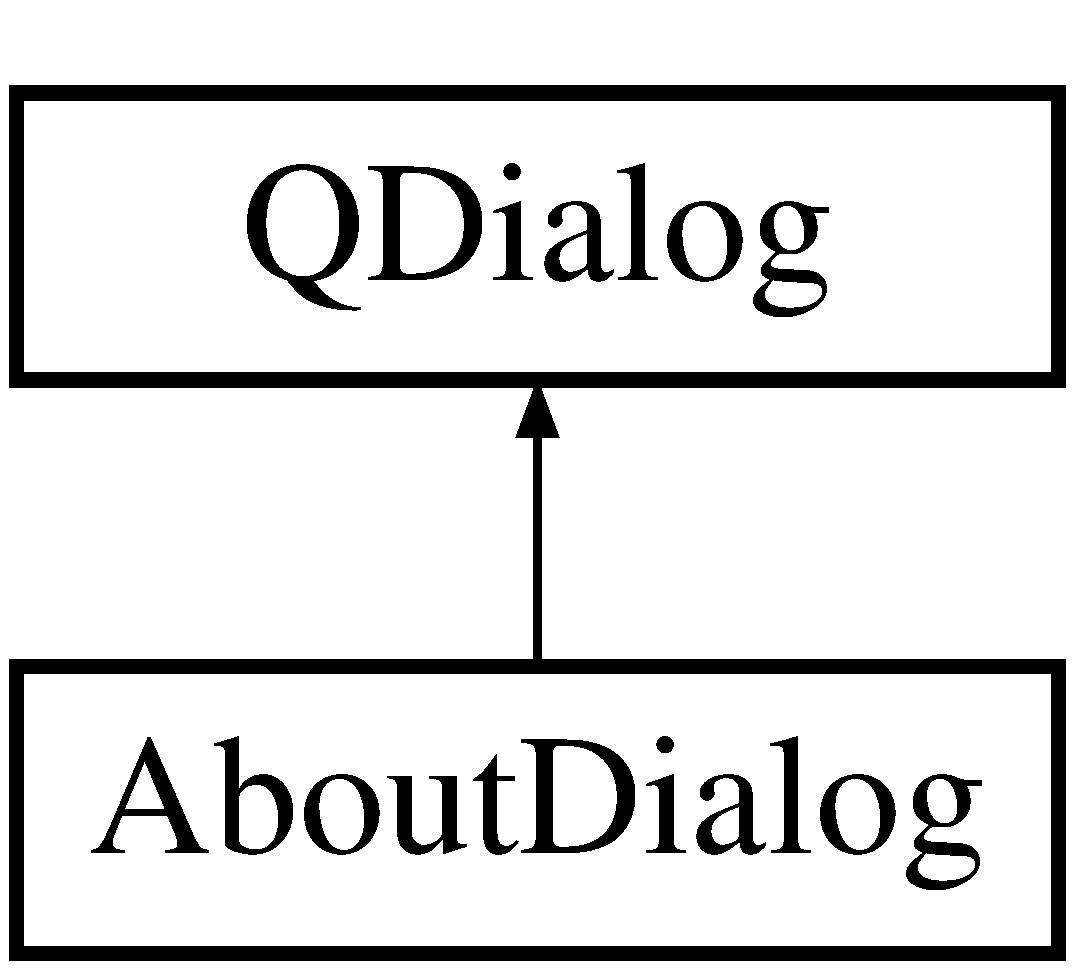
\includegraphics[height=2.000000cm]{classAboutDialog}
\end{center}
\end{figure}
\subsection*{Public Member Functions}
\begin{DoxyCompactItemize}
\item 
\mbox{\Hypertarget{classAboutDialog_ad96fc2ce8de7568ace543b7c69c71c56}\label{classAboutDialog_ad96fc2ce8de7568ace543b7c69c71c56}} 
{\bfseries About\+Dialog} (Q\+Widget $\ast$parent=0)
\end{DoxyCompactItemize}


The documentation for this class was generated from the following files\+:\begin{DoxyCompactItemize}
\item 
src/buildblock/aboutdialog.\+h\item 
src/buildblock/aboutdialog.\+cpp\end{DoxyCompactItemize}

\hypertarget{classAnalysisNema}{}\section{Analysis\+Nema Class Reference}
\label{classAnalysisNema}\index{Analysis\+Nema@{Analysis\+Nema}}
Inheritance diagram for Analysis\+Nema\+:\begin{figure}[H]
\begin{center}
\leavevmode
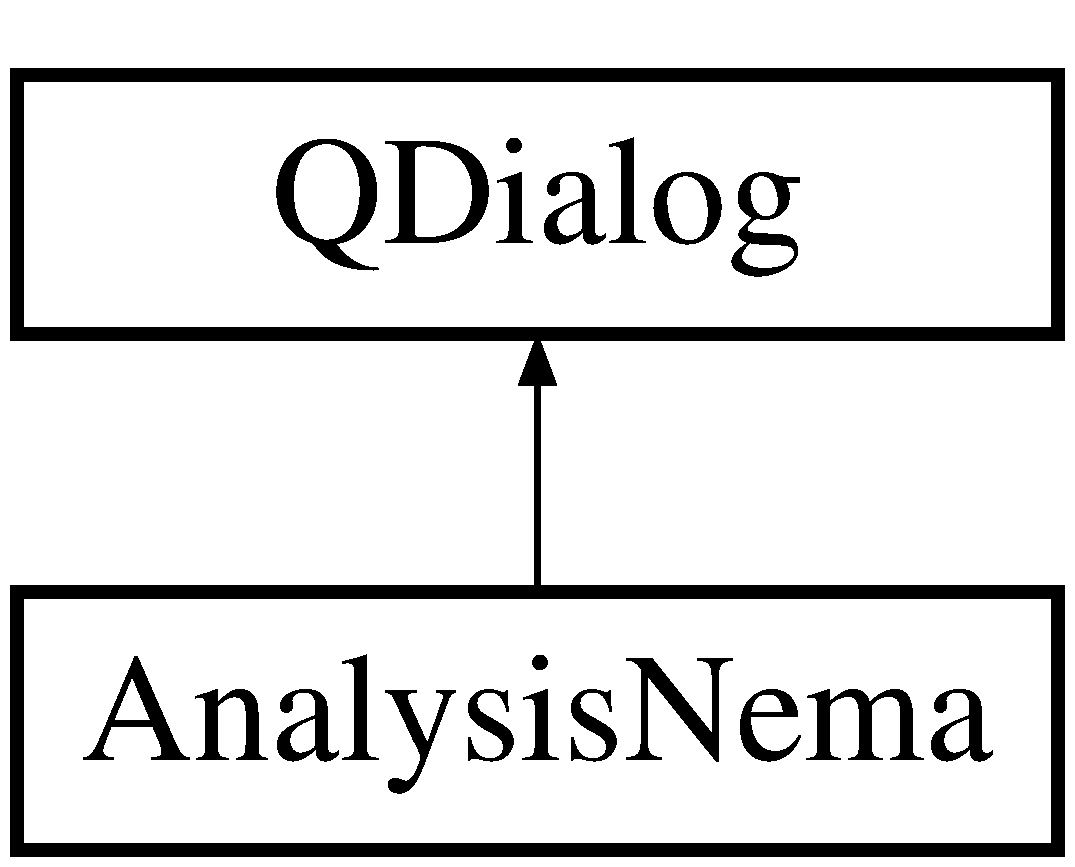
\includegraphics[height=2.000000cm]{classAnalysisNema}
\end{center}
\end{figure}
\subsection*{Public Member Functions}
\begin{DoxyCompactItemize}
\item 
\mbox{\Hypertarget{classAnalysisNema_a22a539a883d51799e5983a40d59fabdf}\label{classAnalysisNema_a22a539a883d51799e5983a40d59fabdf}} 
{\bfseries Analysis\+Nema} (\mbox{\hyperlink{classScreen__manager}{Screen\+\_\+manager}} $\ast$data, Q\+Widget $\ast$parent=0)
\end{DoxyCompactItemize}


The documentation for this class was generated from the following files\+:\begin{DoxyCompactItemize}
\item 
src/ui\+\_\+buildblock/analysisnema.\+h\item 
src/ui\+\_\+buildblock/analysisnema.\+cpp\end{DoxyCompactItemize}

\hypertarget{classBarScreen}{}\section{Bar\+Screen Class Reference}
\label{classBarScreen}\index{Bar\+Screen@{Bar\+Screen}}
Inheritance diagram for Bar\+Screen\+:\begin{figure}[H]
\begin{center}
\leavevmode
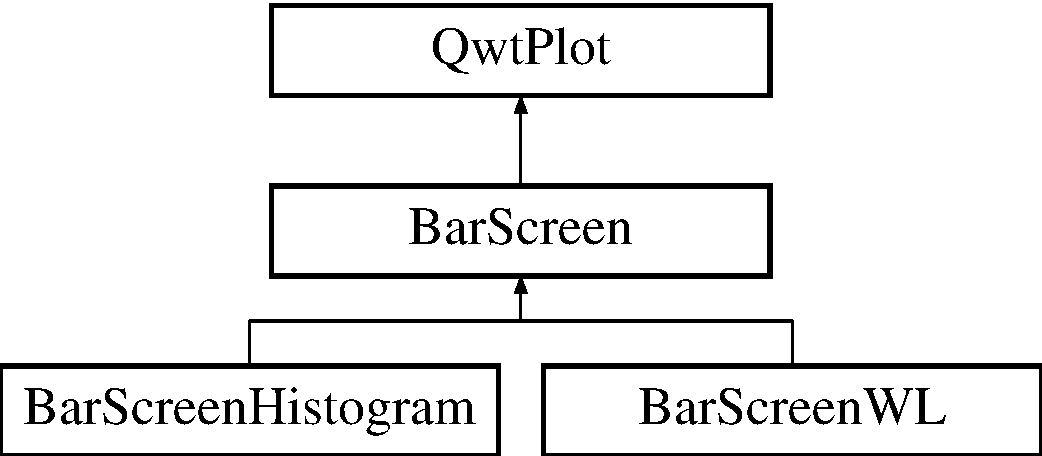
\includegraphics[height=3.000000cm]{classBarScreen}
\end{center}
\end{figure}
\subsection*{Public Slots}
\begin{DoxyCompactItemize}
\item 
\mbox{\Hypertarget{classBarScreen_a73d64473bee2dceb5e14f6ecd9085c5a}\label{classBarScreen_a73d64473bee2dceb5e14f6ecd9085c5a}} 
void {\bfseries unset\+Screen} (bool \+\_\+state)
\item 
\mbox{\Hypertarget{classBarScreen_a584ecbf24a178b74fee22eb40e6281de}\label{classBarScreen_a584ecbf24a178b74fee22eb40e6281de}} 
bool {\bfseries set\+Screen} (Q\+Widget $\ast$, const bool \+\_\+global=false)
\item 
\mbox{\Hypertarget{classBarScreen_a5ced2edf8912f341afaa2fda187be861}\label{classBarScreen_a5ced2edf8912f341afaa2fda187be861}} 
virtual void {\bfseries replot\+\_\+me} ()=0
\end{DoxyCompactItemize}
\subsection*{Signals}
\begin{DoxyCompactItemize}
\item 
\mbox{\Hypertarget{classBarScreen_a39dadd115d8012630aac2ff7cb188fa6}\label{classBarScreen_a39dadd115d8012630aac2ff7cb188fa6}} 
void {\bfseries markers\+Updated} (const float \&, const float \&)
\item 
\mbox{\Hypertarget{classBarScreen_a3251fb8903f71f8ea0df00d17b7302cf}\label{classBarScreen_a3251fb8903f71f8ea0df00d17b7302cf}} 
void {\bfseries WL} (const float \&, const float \&)
\end{DoxyCompactItemize}
\subsection*{Public Member Functions}
\begin{DoxyCompactItemize}
\item 
\mbox{\Hypertarget{classBarScreen_a745463165da3716d2587f9bd15162be4}\label{classBarScreen_a745463165da3716d2587f9bd15162be4}} 
{\bfseries Bar\+Screen} (Q\+Widget $\ast$parent=0, const int \&\+\_\+num\+Bins=16, const float \&\+\_\+cut\+Off=0.\+2f)
\item 
\mbox{\Hypertarget{classBarScreen_a1950f3ff2fcb6f9c815480d79c41bcdd}\label{classBarScreen_a1950f3ff2fcb6f9c815480d79c41bcdd}} 
Q\+Vector$<$ Qwt\+Interval\+Sample $>$\+::iterator {\bfseries get\+\_\+data\+\_\+begin} ()
\item 
\mbox{\Hypertarget{classBarScreen_a8b4c985476a91cfbaba65f9efb2fb98d}\label{classBarScreen_a8b4c985476a91cfbaba65f9efb2fb98d}} 
Q\+Vector$<$ Qwt\+Interval\+Sample $>$\+::iterator {\bfseries get\+\_\+data\+\_\+end} ()
\item 
\mbox{\Hypertarget{classBarScreen_aa39400dbc0e698031f526a5696c5f05e}\label{classBarScreen_aa39400dbc0e698031f526a5696c5f05e}} 
void {\bfseries set\+Num\+Bin} (const int \&\+\_\+n)
\item 
\mbox{\Hypertarget{classBarScreen_a31a0a0513a3506fd31b4921d9ef9de5f}\label{classBarScreen_a31a0a0513a3506fd31b4921d9ef9de5f}} 
void {\bfseries set\+Cut\+Off} (const float \&\+\_\+n)
\item 
\mbox{\Hypertarget{classBarScreen_a3619df2d1013dcd882836654bdc7eca8}\label{classBarScreen_a3619df2d1013dcd882836654bdc7eca8}} 
float {\bfseries get\+Min\+Marker} () const
\item 
\mbox{\Hypertarget{classBarScreen_a8c31c0657a9eae009fae26a6095527af}\label{classBarScreen_a8c31c0657a9eae009fae26a6095527af}} 
float {\bfseries get\+Max\+Marker} () const
\item 
\mbox{\Hypertarget{classBarScreen_a8b1fd79efa17f74f838604cf28e82497}\label{classBarScreen_a8b1fd79efa17f74f838604cf28e82497}} 
float {\bfseries get\+Min\+Value} () const
\item 
\mbox{\Hypertarget{classBarScreen_a6621f8fa1c402d63dd9ac1a29002eb38}\label{classBarScreen_a6621f8fa1c402d63dd9ac1a29002eb38}} 
float {\bfseries get\+Max\+Value} () const
\item 
\mbox{\Hypertarget{classBarScreen_ab9e1489e0b5d95f26fd7a00763e91d11}\label{classBarScreen_ab9e1489e0b5d95f26fd7a00763e91d11}} 
virtual bool {\bfseries set\+Image\+Data} ()
\item 
\mbox{\Hypertarget{classBarScreen_abbb759e28aa304adc0734830fb5d859e}\label{classBarScreen_abbb759e28aa304adc0734830fb5d859e}} 
virtual void {\bfseries move} (Q\+Point to)=0
\item 
\mbox{\Hypertarget{classBarScreen_ab09a99155d2aa5b19baf093129cdf685}\label{classBarScreen_ab09a99155d2aa5b19baf093129cdf685}} 
virtual void {\bfseries move\+Markersby} (Q\+PointF dis)=0
\item 
\mbox{\Hypertarget{classBarScreen_a84c57e7a3258ab5b3f71248d834d1187}\label{classBarScreen_a84c57e7a3258ab5b3f71248d834d1187}} 
virtual void {\bfseries initialise\+Plot\+Area} ()
\item 
\mbox{\Hypertarget{classBarScreen_a3c553483ebb07bd496004d8300eb804f}\label{classBarScreen_a3c553483ebb07bd496004d8300eb804f}} 
Q\+PointF {\bfseries get\+Pointof\+Bin} (const int \&\+\_\+index)
\item 
\mbox{\Hypertarget{classBarScreen_acba5c2bfeac649e5ffdea5255a4537d8}\label{classBarScreen_acba5c2bfeac649e5ffdea5255a4537d8}} 
Q\+PointF {\bfseries get\+Max\+Frequency\+Point} ()
\item 
\mbox{\Hypertarget{classBarScreen_a2a02e1300c43cebc6b61140e7aebc82c}\label{classBarScreen_a2a02e1300c43cebc6b61140e7aebc82c}} 
Q\+PointF {\bfseries get\+Last\+Bin\+Point} ()
\item 
\mbox{\Hypertarget{classBarScreen_aad073d21512c112ca8892e1d7be7b21c}\label{classBarScreen_aad073d21512c112ca8892e1d7be7b21c}} 
double {\bfseries get\+Bin\+Value} (const int \&\+\_\+index)
\item 
\mbox{\Hypertarget{classBarScreen_ab6abcfa2f17cd1abe87f33cd2de73683}\label{classBarScreen_ab6abcfa2f17cd1abe87f33cd2de73683}} 
double {\bfseries get\+Sum} ()
\end{DoxyCompactItemize}
\subsection*{Protected Member Functions}
\begin{DoxyCompactItemize}
\item 
void \mbox{\hyperlink{classBarScreen_ae652343345f7cc3f7726569c1195ee9a}{initialse\+Histogram}} ()
\item 
\mbox{\Hypertarget{classBarScreen_a3e9d73bcf97e00634bf7c8b78d2cbad0}\label{classBarScreen_a3e9d73bcf97e00634bf7c8b78d2cbad0}} 
void \mbox{\hyperlink{classBarScreen_a3e9d73bcf97e00634bf7c8b78d2cbad0}{update\+Histogram}} ()
\begin{DoxyCompactList}\small\item\em Update the histogram. Call this when data are changed. \end{DoxyCompactList}\item 
\mbox{\Hypertarget{classBarScreen_a93cc980ebe50e6d0fb5b62e1715cbc10}\label{classBarScreen_a93cc980ebe50e6d0fb5b62e1715cbc10}} 
virtual void {\bfseries move\+Markers} (const double \&lp, const double \&up)=0
\item 
\mbox{\Hypertarget{classBarScreen_a16448edd7a849d8f64bb1533e42b0c6a}\label{classBarScreen_a16448edd7a849d8f64bb1533e42b0c6a}} 
virtual void {\bfseries draw\+Curve} ()=0
\item 
\mbox{\Hypertarget{classBarScreen_a4d2a43c01c702ce90ffd4433a07d2b73}\label{classBarScreen_a4d2a43c01c702ce90ffd4433a07d2b73}} 
bool {\bfseries unset\+Image\+Data} ()
\end{DoxyCompactItemize}
\subsection*{Protected Attributes}
\begin{DoxyCompactItemize}
\item 
\mbox{\Hypertarget{classBarScreen_a78c84b8c40247d7cb011424250d16ba5}\label{classBarScreen_a78c84b8c40247d7cb011424250d16ba5}} 
\mbox{\hyperlink{classScreen__manager}{Screen\+\_\+manager}} $\ast$ {\bfseries sc}
\item 
\mbox{\Hypertarget{classBarScreen_a5d3193a8e27fd072ed67f069dac1640b}\label{classBarScreen_a5d3193a8e27fd072ed67f069dac1640b}} 
qreal \mbox{\hyperlink{classBarScreen_a5d3193a8e27fd072ed67f069dac1640b}{ll}}
\begin{DoxyCompactList}\small\item\em Lower threshold. \end{DoxyCompactList}\item 
\mbox{\Hypertarget{classBarScreen_a3b456d8140f716cfee488091c927d54f}\label{classBarScreen_a3b456d8140f716cfee488091c927d54f}} 
qreal \mbox{\hyperlink{classBarScreen_a3b456d8140f716cfee488091c927d54f}{uu}}
\begin{DoxyCompactList}\small\item\em Upper threshold. \end{DoxyCompactList}\item 
\mbox{\Hypertarget{classBarScreen_a3d5a447b9895c22cf4e28ea041cef272}\label{classBarScreen_a3d5a447b9895c22cf4e28ea041cef272}} 
std\+::unique\+\_\+ptr$<$ Q\+PointF $>$ {\bfseries min\+Marker}
\item 
\mbox{\Hypertarget{classBarScreen_a80404aaebe17ccccf1918c8f7b59dc3e}\label{classBarScreen_a80404aaebe17ccccf1918c8f7b59dc3e}} 
std\+::unique\+\_\+ptr$<$ Q\+PointF $>$ {\bfseries max\+Marker}
\item 
\mbox{\Hypertarget{classBarScreen_a92a1082b85912224f43a4f2ea85aa289}\label{classBarScreen_a92a1082b85912224f43a4f2ea85aa289}} 
gsl\+\_\+histogram $\ast$ {\bfseries h}
\item 
\mbox{\Hypertarget{classBarScreen_ad590da057a164a1d8a5339243165adf7}\label{classBarScreen_ad590da057a164a1d8a5339243165adf7}} 
Qwt\+Plot\+Curve $\ast$ {\bfseries curve}
\item 
\mbox{\Hypertarget{classBarScreen_a760794dcf754291e8048d11b59f164c4}\label{classBarScreen_a760794dcf754291e8048d11b59f164c4}} 
qint8 {\bfseries state}
\item 
\mbox{\Hypertarget{classBarScreen_ae1d1f7ad5265d8cab9cfb4508060d888}\label{classBarScreen_ae1d1f7ad5265d8cab9cfb4508060d888}} 
Qwt\+Plot\+Histogram $\ast$ {\bfseries d\+\_\+hist\+Item}
\item 
\mbox{\Hypertarget{classBarScreen_a0521180a30d14315bc7a98471d616392}\label{classBarScreen_a0521180a30d14315bc7a98471d616392}} 
Q\+Vector$<$ Qwt\+Interval\+Sample $>$ {\bfseries series}
\item 
\mbox{\Hypertarget{classBarScreen_a76549683ce4069172a98f3166a24cec7}\label{classBarScreen_a76549683ce4069172a98f3166a24cec7}} 
Q\+Vector$<$ Qwt\+Interval $>$ {\bfseries intervalA}
\item 
\mbox{\Hypertarget{classBarScreen_a87fe5a37838e56362f08d5a58f60342f}\label{classBarScreen_a87fe5a37838e56362f08d5a58f60342f}} 
int {\bfseries num\+Bins}
\item 
\mbox{\Hypertarget{classBarScreen_abeadea18d6006cdf5a0d0a8f4f757d8f}\label{classBarScreen_abeadea18d6006cdf5a0d0a8f4f757d8f}} 
float {\bfseries cut\+Off}
\item 
\mbox{\Hypertarget{classBarScreen_ac4309c85d480f5a3d706082824983b66}\label{classBarScreen_ac4309c85d480f5a3d706082824983b66}} 
double {\bfseries def\+\_\+min}
\item 
\mbox{\Hypertarget{classBarScreen_a84c112218b1ba0d4c1b7d1f686719f6a}\label{classBarScreen_a84c112218b1ba0d4c1b7d1f686719f6a}} 
double {\bfseries def\+\_\+max}
\item 
\mbox{\Hypertarget{classBarScreen_a3a27d451636712e1753eaf2db3f85f15}\label{classBarScreen_a3a27d451636712e1753eaf2db3f85f15}} 
double {\bfseries range}
\item 
\mbox{\Hypertarget{classBarScreen_a2cb90ccb8dcd7b33d9080a449de15078}\label{classBarScreen_a2cb90ccb8dcd7b33d9080a449de15078}} 
double {\bfseries cc}
\item 
\mbox{\Hypertarget{classBarScreen_ac8a4ecb5610b79c443fbcb6e062b57ff}\label{classBarScreen_ac8a4ecb5610b79c443fbcb6e062b57ff}} 
Q\+Point {\bfseries cog}
\item 
\mbox{\Hypertarget{classBarScreen_a08aebf344206b301e0c33b6115e5c485}\label{classBarScreen_a08aebf344206b301e0c33b6115e5c485}} 
Q\+Pixmap {\bfseries cursor\+\_\+pixmap}
\item 
\mbox{\Hypertarget{classBarScreen_a2be28f5fb73a79676c840fa62a482c63}\label{classBarScreen_a2be28f5fb73a79676c840fa62a482c63}} 
Qwt\+Symbol $\ast$ {\bfseries d}
\item 
\mbox{\Hypertarget{classBarScreen_a93ef91eff5bcac1a17ccb7b5a4811368}\label{classBarScreen_a93ef91eff5bcac1a17ccb7b5a4811368}} 
float \mbox{\hyperlink{classBarScreen_a93ef91eff5bcac1a17ccb7b5a4811368}{nz\+\_\+max}}
\begin{DoxyCompactList}\small\item\em The max of all bins excluding the first bin, which includes the voxels with value 0. \end{DoxyCompactList}\item 
\mbox{\Hypertarget{classBarScreen_adf2fa1b3686c92bd20e8c0befc06caf7}\label{classBarScreen_adf2fa1b3686c92bd20e8c0befc06caf7}} 
float \mbox{\hyperlink{classBarScreen_adf2fa1b3686c92bd20e8c0befc06caf7}{nz\+\_\+sum}}
\begin{DoxyCompactList}\small\item\em The sum of all bins excluding the first bin, which includes the voxels with value 0. \end{DoxyCompactList}\item 
\mbox{\Hypertarget{classBarScreen_a2222951d5a5ce44bb22da49e62e8f797}\label{classBarScreen_a2222951d5a5ce44bb22da49e62e8f797}} 
bool \mbox{\hyperlink{classBarScreen_a2222951d5a5ce44bb22da49e62e8f797}{linked}}
\begin{DoxyCompactList}\small\item\em Start listening of events afther an image has been set. \end{DoxyCompactList}\item 
\mbox{\Hypertarget{classBarScreen_a3c0cbb54bb95017b259687ee79232a08}\label{classBarScreen_a3c0cbb54bb95017b259687ee79232a08}} 
bool {\bfseries global\+Hist}
\end{DoxyCompactItemize}


\subsection{Member Function Documentation}
\mbox{\Hypertarget{classBarScreen_ae652343345f7cc3f7726569c1195ee9a}\label{classBarScreen_ae652343345f7cc3f7726569c1195ee9a}} 
\index{Bar\+Screen@{Bar\+Screen}!initialse\+Histogram@{initialse\+Histogram}}
\index{initialse\+Histogram@{initialse\+Histogram}!Bar\+Screen@{Bar\+Screen}}
\subsubsection{\texorpdfstring{initialse\+Histogram()}{initialseHistogram()}}
{\footnotesize\ttfamily void Bar\+Screen\+::initialse\+Histogram (\begin{DoxyParamCaption}{ }\end{DoxyParamCaption})\hspace{0.3cm}{\ttfamily [protected]}}

Intialises the histogram. Should be called when changes on the num\+Bins or the data occur. 

The documentation for this class was generated from the following files\+:\begin{DoxyCompactItemize}
\item 
src/display\+\_\+buildblock/bar\+\_\+screen.\+h\item 
src/display\+\_\+buildblock/bar\+\_\+screen.\+cpp\end{DoxyCompactItemize}

\hypertarget{classBarScreenHistogram}{}\section{Bar\+Screen\+Histogram Class Reference}
\label{classBarScreenHistogram}\index{Bar\+Screen\+Histogram@{Bar\+Screen\+Histogram}}
Inheritance diagram for Bar\+Screen\+Histogram\+:\begin{figure}[H]
\begin{center}
\leavevmode
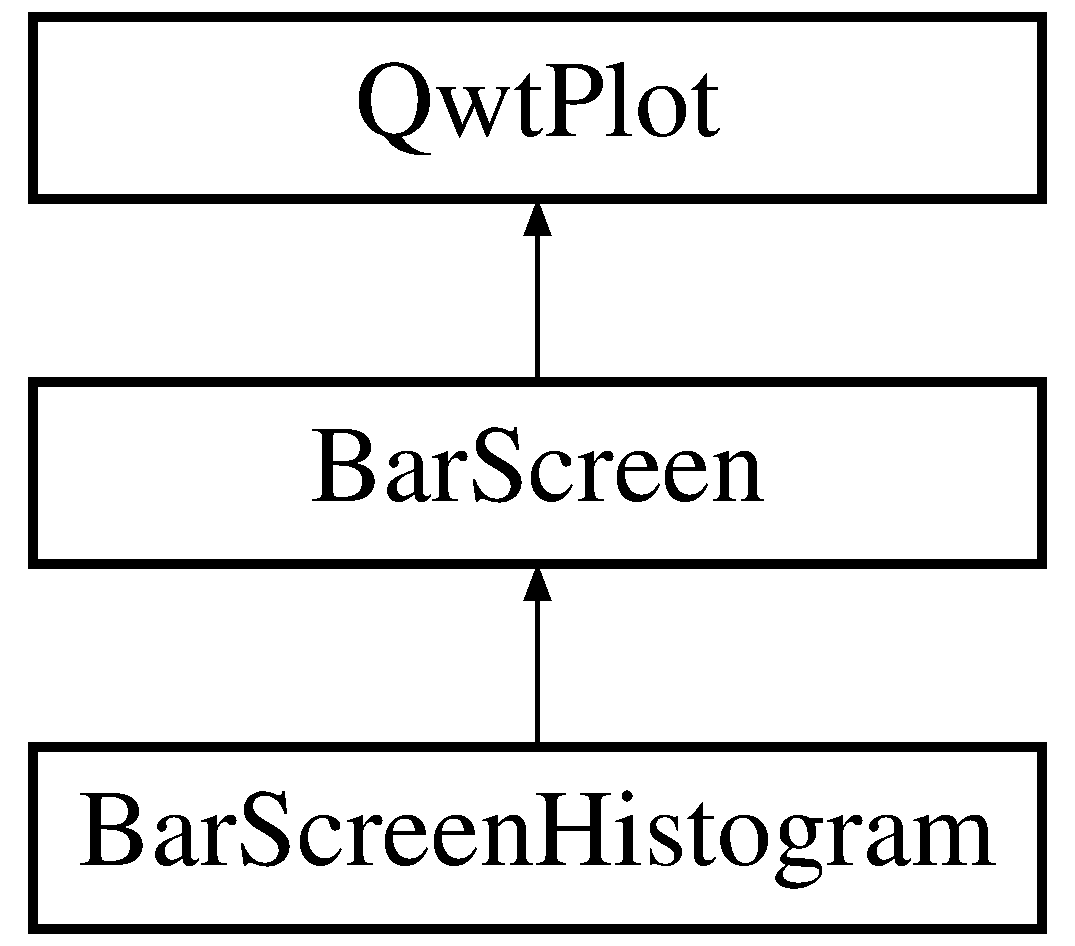
\includegraphics[height=3.000000cm]{classBarScreenHistogram}
\end{center}
\end{figure}
\subsection*{Public Slots}
\begin{DoxyCompactItemize}
\item 
\mbox{\Hypertarget{classBarScreenHistogram_a8a9a46d20f80b4ff1a8225f164651ce4}\label{classBarScreenHistogram_a8a9a46d20f80b4ff1a8225f164651ce4}} 
void {\bfseries replot\+\_\+me} ()
\item 
\mbox{\Hypertarget{classBarScreen_a73d64473bee2dceb5e14f6ecd9085c5a}\label{classBarScreen_a73d64473bee2dceb5e14f6ecd9085c5a}} 
void {\bfseries unset\+Screen} (bool \+\_\+state)
\item 
\mbox{\Hypertarget{classBarScreen_a584ecbf24a178b74fee22eb40e6281de}\label{classBarScreen_a584ecbf24a178b74fee22eb40e6281de}} 
bool {\bfseries set\+Screen} (Q\+Widget $\ast$, const bool \+\_\+global=false)
\end{DoxyCompactItemize}
\subsection*{Signals}
\begin{DoxyCompactItemize}
\item 
\mbox{\Hypertarget{classBarScreen_a39dadd115d8012630aac2ff7cb188fa6}\label{classBarScreen_a39dadd115d8012630aac2ff7cb188fa6}} 
void {\bfseries markers\+Updated} (const float \&, const float \&)
\item 
\mbox{\Hypertarget{classBarScreen_a3251fb8903f71f8ea0df00d17b7302cf}\label{classBarScreen_a3251fb8903f71f8ea0df00d17b7302cf}} 
void {\bfseries WL} (const float \&, const float \&)
\end{DoxyCompactItemize}
\subsection*{Public Member Functions}
\begin{DoxyCompactItemize}
\item 
\mbox{\Hypertarget{classBarScreenHistogram_aa3cc6d1640882d3d16207abdf1d920d5}\label{classBarScreenHistogram_aa3cc6d1640882d3d16207abdf1d920d5}} 
{\bfseries Bar\+Screen\+Histogram} (Q\+Widget $\ast$parent=0)
\item 
\mbox{\Hypertarget{classBarScreenHistogram_a7bbde2d9c8da75756d9caf5c3dd40ca0}\label{classBarScreenHistogram_a7bbde2d9c8da75756d9caf5c3dd40ca0}} 
void {\bfseries initialise\+Plot\+Area} ()
\item 
\mbox{\Hypertarget{classBarScreenHistogram_a0be353de9471e4b7b77626e37d273841}\label{classBarScreenHistogram_a0be353de9471e4b7b77626e37d273841}} 
void {\bfseries move\+Markersby} (Q\+PointF dis)
\item 
\mbox{\Hypertarget{classBarScreenHistogram_afdce5fc9b8f8fbcc5c12dd3344dad78d}\label{classBarScreenHistogram_afdce5fc9b8f8fbcc5c12dd3344dad78d}} 
void {\bfseries move} (Q\+Point to)
\item 
\mbox{\Hypertarget{classBarScreenHistogram_ac0df6530441f3cc48bc1609baf59cb6f}\label{classBarScreenHistogram_ac0df6530441f3cc48bc1609baf59cb6f}} 
virtual bool {\bfseries event} (Q\+Event $\ast$)
\item 
\mbox{\Hypertarget{classBarScreenHistogram_a325533d70611598df0ab5c079b1b59fd}\label{classBarScreenHistogram_a325533d70611598df0ab5c079b1b59fd}} 
void {\bfseries set\+Threshold} (const float \&\+\_\+f)
\item 
\mbox{\Hypertarget{classBarScreen_a1950f3ff2fcb6f9c815480d79c41bcdd}\label{classBarScreen_a1950f3ff2fcb6f9c815480d79c41bcdd}} 
Q\+Vector$<$ Qwt\+Interval\+Sample $>$\+::iterator {\bfseries get\+\_\+data\+\_\+begin} ()
\item 
\mbox{\Hypertarget{classBarScreen_a8b4c985476a91cfbaba65f9efb2fb98d}\label{classBarScreen_a8b4c985476a91cfbaba65f9efb2fb98d}} 
Q\+Vector$<$ Qwt\+Interval\+Sample $>$\+::iterator {\bfseries get\+\_\+data\+\_\+end} ()
\item 
\mbox{\Hypertarget{classBarScreen_aa39400dbc0e698031f526a5696c5f05e}\label{classBarScreen_aa39400dbc0e698031f526a5696c5f05e}} 
void {\bfseries set\+Num\+Bin} (const int \&\+\_\+n)
\item 
\mbox{\Hypertarget{classBarScreen_a31a0a0513a3506fd31b4921d9ef9de5f}\label{classBarScreen_a31a0a0513a3506fd31b4921d9ef9de5f}} 
void {\bfseries set\+Cut\+Off} (const float \&\+\_\+n)
\item 
\mbox{\Hypertarget{classBarScreen_a3619df2d1013dcd882836654bdc7eca8}\label{classBarScreen_a3619df2d1013dcd882836654bdc7eca8}} 
float {\bfseries get\+Min\+Marker} () const
\item 
\mbox{\Hypertarget{classBarScreen_a8c31c0657a9eae009fae26a6095527af}\label{classBarScreen_a8c31c0657a9eae009fae26a6095527af}} 
float {\bfseries get\+Max\+Marker} () const
\item 
\mbox{\Hypertarget{classBarScreen_a8b1fd79efa17f74f838604cf28e82497}\label{classBarScreen_a8b1fd79efa17f74f838604cf28e82497}} 
float {\bfseries get\+Min\+Value} () const
\item 
\mbox{\Hypertarget{classBarScreen_a6621f8fa1c402d63dd9ac1a29002eb38}\label{classBarScreen_a6621f8fa1c402d63dd9ac1a29002eb38}} 
float {\bfseries get\+Max\+Value} () const
\item 
\mbox{\Hypertarget{classBarScreen_ab9e1489e0b5d95f26fd7a00763e91d11}\label{classBarScreen_ab9e1489e0b5d95f26fd7a00763e91d11}} 
virtual bool {\bfseries set\+Image\+Data} ()
\item 
\mbox{\Hypertarget{classBarScreen_a3c553483ebb07bd496004d8300eb804f}\label{classBarScreen_a3c553483ebb07bd496004d8300eb804f}} 
Q\+PointF {\bfseries get\+Pointof\+Bin} (const int \&\+\_\+index)
\item 
\mbox{\Hypertarget{classBarScreen_acba5c2bfeac649e5ffdea5255a4537d8}\label{classBarScreen_acba5c2bfeac649e5ffdea5255a4537d8}} 
Q\+PointF {\bfseries get\+Max\+Frequency\+Point} ()
\item 
\mbox{\Hypertarget{classBarScreen_a2a02e1300c43cebc6b61140e7aebc82c}\label{classBarScreen_a2a02e1300c43cebc6b61140e7aebc82c}} 
Q\+PointF {\bfseries get\+Last\+Bin\+Point} ()
\item 
\mbox{\Hypertarget{classBarScreen_aad073d21512c112ca8892e1d7be7b21c}\label{classBarScreen_aad073d21512c112ca8892e1d7be7b21c}} 
double {\bfseries get\+Bin\+Value} (const int \&\+\_\+index)
\item 
\mbox{\Hypertarget{classBarScreen_ab6abcfa2f17cd1abe87f33cd2de73683}\label{classBarScreen_ab6abcfa2f17cd1abe87f33cd2de73683}} 
double {\bfseries get\+Sum} ()
\end{DoxyCompactItemize}
\subsection*{Protected Member Functions}
\begin{DoxyCompactItemize}
\item 
\mbox{\Hypertarget{classBarScreenHistogram_af87a78ee267e6361ae73cf61845b31d6}\label{classBarScreenHistogram_af87a78ee267e6361ae73cf61845b31d6}} 
void {\bfseries draw\+Curve} ()
\item 
\mbox{\Hypertarget{classBarScreenHistogram_a49b7afd95b207b1fa146d6e14dfde4a5}\label{classBarScreenHistogram_a49b7afd95b207b1fa146d6e14dfde4a5}} 
virtual void {\bfseries move\+Markers} (const double \&lp, const double \&up)
\item 
void \mbox{\hyperlink{classBarScreen_ae652343345f7cc3f7726569c1195ee9a}{initialse\+Histogram}} ()
\item 
\mbox{\Hypertarget{classBarScreen_a3e9d73bcf97e00634bf7c8b78d2cbad0}\label{classBarScreen_a3e9d73bcf97e00634bf7c8b78d2cbad0}} 
void \mbox{\hyperlink{classBarScreen_a3e9d73bcf97e00634bf7c8b78d2cbad0}{update\+Histogram}} ()
\begin{DoxyCompactList}\small\item\em Update the histogram. Call this when data are changed. \end{DoxyCompactList}\item 
\mbox{\Hypertarget{classBarScreen_a4d2a43c01c702ce90ffd4433a07d2b73}\label{classBarScreen_a4d2a43c01c702ce90ffd4433a07d2b73}} 
bool {\bfseries unset\+Image\+Data} ()
\end{DoxyCompactItemize}
\subsection*{Protected Attributes}
\begin{DoxyCompactItemize}
\item 
\mbox{\Hypertarget{classBarScreen_a78c84b8c40247d7cb011424250d16ba5}\label{classBarScreen_a78c84b8c40247d7cb011424250d16ba5}} 
\mbox{\hyperlink{classScreen__manager}{Screen\+\_\+manager}} $\ast$ {\bfseries sc}
\item 
\mbox{\Hypertarget{classBarScreen_a5d3193a8e27fd072ed67f069dac1640b}\label{classBarScreen_a5d3193a8e27fd072ed67f069dac1640b}} 
qreal \mbox{\hyperlink{classBarScreen_a5d3193a8e27fd072ed67f069dac1640b}{ll}}
\begin{DoxyCompactList}\small\item\em Lower threshold. \end{DoxyCompactList}\item 
\mbox{\Hypertarget{classBarScreen_a3b456d8140f716cfee488091c927d54f}\label{classBarScreen_a3b456d8140f716cfee488091c927d54f}} 
qreal \mbox{\hyperlink{classBarScreen_a3b456d8140f716cfee488091c927d54f}{uu}}
\begin{DoxyCompactList}\small\item\em Upper threshold. \end{DoxyCompactList}\item 
\mbox{\Hypertarget{classBarScreen_a3d5a447b9895c22cf4e28ea041cef272}\label{classBarScreen_a3d5a447b9895c22cf4e28ea041cef272}} 
std\+::unique\+\_\+ptr$<$ Q\+PointF $>$ {\bfseries min\+Marker}
\item 
\mbox{\Hypertarget{classBarScreen_a80404aaebe17ccccf1918c8f7b59dc3e}\label{classBarScreen_a80404aaebe17ccccf1918c8f7b59dc3e}} 
std\+::unique\+\_\+ptr$<$ Q\+PointF $>$ {\bfseries max\+Marker}
\item 
\mbox{\Hypertarget{classBarScreen_a92a1082b85912224f43a4f2ea85aa289}\label{classBarScreen_a92a1082b85912224f43a4f2ea85aa289}} 
gsl\+\_\+histogram $\ast$ {\bfseries h}
\item 
\mbox{\Hypertarget{classBarScreen_ad590da057a164a1d8a5339243165adf7}\label{classBarScreen_ad590da057a164a1d8a5339243165adf7}} 
Qwt\+Plot\+Curve $\ast$ {\bfseries curve}
\item 
\mbox{\Hypertarget{classBarScreen_a760794dcf754291e8048d11b59f164c4}\label{classBarScreen_a760794dcf754291e8048d11b59f164c4}} 
qint8 {\bfseries state}
\item 
\mbox{\Hypertarget{classBarScreen_ae1d1f7ad5265d8cab9cfb4508060d888}\label{classBarScreen_ae1d1f7ad5265d8cab9cfb4508060d888}} 
Qwt\+Plot\+Histogram $\ast$ {\bfseries d\+\_\+hist\+Item}
\item 
\mbox{\Hypertarget{classBarScreen_a0521180a30d14315bc7a98471d616392}\label{classBarScreen_a0521180a30d14315bc7a98471d616392}} 
Q\+Vector$<$ Qwt\+Interval\+Sample $>$ {\bfseries series}
\item 
\mbox{\Hypertarget{classBarScreen_a76549683ce4069172a98f3166a24cec7}\label{classBarScreen_a76549683ce4069172a98f3166a24cec7}} 
Q\+Vector$<$ Qwt\+Interval $>$ {\bfseries intervalA}
\item 
\mbox{\Hypertarget{classBarScreen_a87fe5a37838e56362f08d5a58f60342f}\label{classBarScreen_a87fe5a37838e56362f08d5a58f60342f}} 
int {\bfseries num\+Bins}
\item 
\mbox{\Hypertarget{classBarScreen_abeadea18d6006cdf5a0d0a8f4f757d8f}\label{classBarScreen_abeadea18d6006cdf5a0d0a8f4f757d8f}} 
float {\bfseries cut\+Off}
\item 
\mbox{\Hypertarget{classBarScreen_ac4309c85d480f5a3d706082824983b66}\label{classBarScreen_ac4309c85d480f5a3d706082824983b66}} 
double {\bfseries def\+\_\+min}
\item 
\mbox{\Hypertarget{classBarScreen_a84c112218b1ba0d4c1b7d1f686719f6a}\label{classBarScreen_a84c112218b1ba0d4c1b7d1f686719f6a}} 
double {\bfseries def\+\_\+max}
\item 
\mbox{\Hypertarget{classBarScreen_a3a27d451636712e1753eaf2db3f85f15}\label{classBarScreen_a3a27d451636712e1753eaf2db3f85f15}} 
double {\bfseries range}
\item 
\mbox{\Hypertarget{classBarScreen_a2cb90ccb8dcd7b33d9080a449de15078}\label{classBarScreen_a2cb90ccb8dcd7b33d9080a449de15078}} 
double {\bfseries cc}
\item 
\mbox{\Hypertarget{classBarScreen_ac8a4ecb5610b79c443fbcb6e062b57ff}\label{classBarScreen_ac8a4ecb5610b79c443fbcb6e062b57ff}} 
Q\+Point {\bfseries cog}
\item 
\mbox{\Hypertarget{classBarScreen_a08aebf344206b301e0c33b6115e5c485}\label{classBarScreen_a08aebf344206b301e0c33b6115e5c485}} 
Q\+Pixmap {\bfseries cursor\+\_\+pixmap}
\item 
\mbox{\Hypertarget{classBarScreen_a2be28f5fb73a79676c840fa62a482c63}\label{classBarScreen_a2be28f5fb73a79676c840fa62a482c63}} 
Qwt\+Symbol $\ast$ {\bfseries d}
\item 
\mbox{\Hypertarget{classBarScreen_a93ef91eff5bcac1a17ccb7b5a4811368}\label{classBarScreen_a93ef91eff5bcac1a17ccb7b5a4811368}} 
float \mbox{\hyperlink{classBarScreen_a93ef91eff5bcac1a17ccb7b5a4811368}{nz\+\_\+max}}
\begin{DoxyCompactList}\small\item\em The max of all bins excluding the first bin, which includes the voxels with value 0. \end{DoxyCompactList}\item 
\mbox{\Hypertarget{classBarScreen_adf2fa1b3686c92bd20e8c0befc06caf7}\label{classBarScreen_adf2fa1b3686c92bd20e8c0befc06caf7}} 
float \mbox{\hyperlink{classBarScreen_adf2fa1b3686c92bd20e8c0befc06caf7}{nz\+\_\+sum}}
\begin{DoxyCompactList}\small\item\em The sum of all bins excluding the first bin, which includes the voxels with value 0. \end{DoxyCompactList}\item 
\mbox{\Hypertarget{classBarScreen_a2222951d5a5ce44bb22da49e62e8f797}\label{classBarScreen_a2222951d5a5ce44bb22da49e62e8f797}} 
bool \mbox{\hyperlink{classBarScreen_a2222951d5a5ce44bb22da49e62e8f797}{linked}}
\begin{DoxyCompactList}\small\item\em Start listening of events afther an image has been set. \end{DoxyCompactList}\item 
\mbox{\Hypertarget{classBarScreen_a3c0cbb54bb95017b259687ee79232a08}\label{classBarScreen_a3c0cbb54bb95017b259687ee79232a08}} 
bool {\bfseries global\+Hist}
\end{DoxyCompactItemize}


\subsection{Member Function Documentation}
\mbox{\Hypertarget{classBarScreen_ae652343345f7cc3f7726569c1195ee9a}\label{classBarScreen_ae652343345f7cc3f7726569c1195ee9a}} 
\index{Bar\+Screen\+Histogram@{Bar\+Screen\+Histogram}!initialse\+Histogram@{initialse\+Histogram}}
\index{initialse\+Histogram@{initialse\+Histogram}!Bar\+Screen\+Histogram@{Bar\+Screen\+Histogram}}
\subsubsection{\texorpdfstring{initialse\+Histogram()}{initialseHistogram()}}
{\footnotesize\ttfamily void Bar\+Screen\+::initialse\+Histogram (\begin{DoxyParamCaption}{ }\end{DoxyParamCaption})\hspace{0.3cm}{\ttfamily [protected]}, {\ttfamily [inherited]}}

Intialises the histogram. Should be called when changes on the num\+Bins or the data occur. 

The documentation for this class was generated from the following files\+:\begin{DoxyCompactItemize}
\item 
src/display\+\_\+buildblock/barscreenhistogram.\+h\item 
src/display\+\_\+buildblock/barscreenhistogram.\+cpp\end{DoxyCompactItemize}

\hypertarget{classBarScreenWL}{}\section{Bar\+Screen\+WL Class Reference}
\label{classBarScreenWL}\index{Bar\+Screen\+WL@{Bar\+Screen\+WL}}
Inheritance diagram for Bar\+Screen\+WL\+:\begin{figure}[H]
\begin{center}
\leavevmode
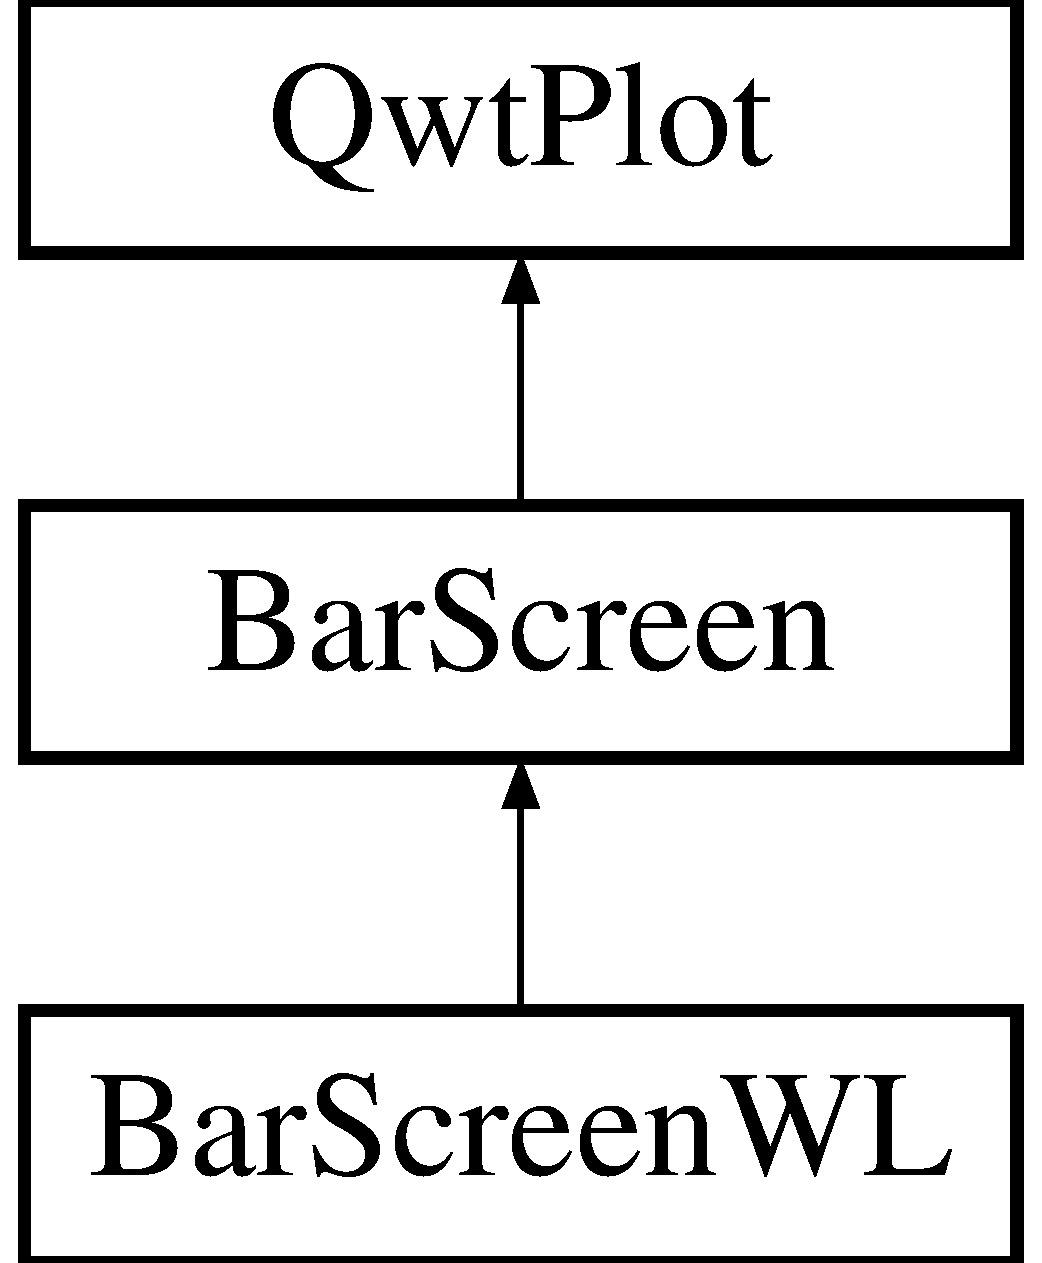
\includegraphics[height=3.000000cm]{classBarScreenWL}
\end{center}
\end{figure}
\subsection*{Public Slots}
\begin{DoxyCompactItemize}
\item 
\mbox{\Hypertarget{classBarScreenWL_afe0474598cdfc4ed117c6f7300a90a92}\label{classBarScreenWL_afe0474598cdfc4ed117c6f7300a90a92}} 
void \mbox{\hyperlink{classBarScreenWL_afe0474598cdfc4ed117c6f7300a90a92}{replot\+\_\+me}} ()
\begin{DoxyCompactList}\small\item\em This is called when the data have been changed. \end{DoxyCompactList}\item 
\mbox{\Hypertarget{classBarScreen_a73d64473bee2dceb5e14f6ecd9085c5a}\label{classBarScreen_a73d64473bee2dceb5e14f6ecd9085c5a}} 
void {\bfseries unset\+Screen} (bool \+\_\+state)
\item 
\mbox{\Hypertarget{classBarScreen_a584ecbf24a178b74fee22eb40e6281de}\label{classBarScreen_a584ecbf24a178b74fee22eb40e6281de}} 
bool {\bfseries set\+Screen} (Q\+Widget $\ast$, const bool \+\_\+global=false)
\end{DoxyCompactItemize}
\subsection*{Signals}
\begin{DoxyCompactItemize}
\item 
\mbox{\Hypertarget{classBarScreen_a39dadd115d8012630aac2ff7cb188fa6}\label{classBarScreen_a39dadd115d8012630aac2ff7cb188fa6}} 
void {\bfseries markers\+Updated} (const float \&, const float \&)
\item 
\mbox{\Hypertarget{classBarScreen_a3251fb8903f71f8ea0df00d17b7302cf}\label{classBarScreen_a3251fb8903f71f8ea0df00d17b7302cf}} 
void {\bfseries WL} (const float \&, const float \&)
\end{DoxyCompactItemize}
\subsection*{Public Member Functions}
\begin{DoxyCompactItemize}
\item 
\mbox{\Hypertarget{classBarScreenWL_a361e5d99c9ba639e5caa053bb5f161e0}\label{classBarScreenWL_a361e5d99c9ba639e5caa053bb5f161e0}} 
{\bfseries Bar\+Screen\+WL} (Q\+Widget $\ast$parent=0)
\item 
\mbox{\Hypertarget{classBarScreenWL_a6f4e3adc277e51b8fc427a06ee0c494d}\label{classBarScreenWL_a6f4e3adc277e51b8fc427a06ee0c494d}} 
void {\bfseries set\+Window} (const float \&\+\_\+m)
\item 
\mbox{\Hypertarget{classBarScreenWL_a23531a0e46637ef6fbbfe5c192521cd2}\label{classBarScreenWL_a23531a0e46637ef6fbbfe5c192521cd2}} 
void {\bfseries set\+Level} (const float \&\+\_\+m)
\item 
\mbox{\Hypertarget{classBarScreenWL_a3130db616461fb3e9db9b54188d2715b}\label{classBarScreenWL_a3130db616461fb3e9db9b54188d2715b}} 
void {\bfseries initialise\+Plot\+Area} ()
\item 
\mbox{\Hypertarget{classBarScreenWL_aac2ca60412c5718c354191b2e8d8ddc9}\label{classBarScreenWL_aac2ca60412c5718c354191b2e8d8ddc9}} 
void {\bfseries move} (Q\+Point to)
\item 
\mbox{\Hypertarget{classBarScreenWL_a6a7085d5b14f17255b4724eb011b3e57}\label{classBarScreenWL_a6a7085d5b14f17255b4724eb011b3e57}} 
void {\bfseries move\+Markersby} (Q\+PointF dis)
\item 
\mbox{\Hypertarget{classBarScreenWL_a1b374e47c58463d100823d9a10efa98a}\label{classBarScreenWL_a1b374e47c58463d100823d9a10efa98a}} 
float {\bfseries get\+Window} () const
\item 
\mbox{\Hypertarget{classBarScreenWL_a9ad0bab5b89b52d377c4fd835411cbc0}\label{classBarScreenWL_a9ad0bab5b89b52d377c4fd835411cbc0}} 
float {\bfseries get\+Level} () const
\item 
\mbox{\Hypertarget{classBarScreenWL_ac881bb98cc168be4ec5a85b7eec08998}\label{classBarScreenWL_ac881bb98cc168be4ec5a85b7eec08998}} 
void {\bfseries set\+Min\+Marker} (const float \&\+\_\+m)
\item 
\mbox{\Hypertarget{classBarScreenWL_ac4924b94bdf8b03a4cdf401e9e5692c4}\label{classBarScreenWL_ac4924b94bdf8b03a4cdf401e9e5692c4}} 
void {\bfseries set\+Max\+Marker} (const float \&\+\_\+m)
\item 
\mbox{\Hypertarget{classBarScreenWL_a3a2f5fd225168fe850d08d57a7d46e23}\label{classBarScreenWL_a3a2f5fd225168fe850d08d57a7d46e23}} 
virtual bool {\bfseries event} (Q\+Event $\ast$)
\item 
\mbox{\Hypertarget{classBarScreenWL_a6fe94b0eae1c5fb513837b7cf424b67f}\label{classBarScreenWL_a6fe94b0eae1c5fb513837b7cf424b67f}} 
void {\bfseries set\+C\+OG} (Q\+Point \+\_\+cog)
\item 
\mbox{\Hypertarget{classBarScreenWL_af1d50a882140b7dbfe27aaa08f54e903}\label{classBarScreenWL_af1d50a882140b7dbfe27aaa08f54e903}} 
void {\bfseries reset\+C\+OG} (int \+\_\+state=-\/1)
\item 
\mbox{\Hypertarget{classBarScreen_a1950f3ff2fcb6f9c815480d79c41bcdd}\label{classBarScreen_a1950f3ff2fcb6f9c815480d79c41bcdd}} 
Q\+Vector$<$ Qwt\+Interval\+Sample $>$\+::iterator {\bfseries get\+\_\+data\+\_\+begin} ()
\item 
\mbox{\Hypertarget{classBarScreen_a8b4c985476a91cfbaba65f9efb2fb98d}\label{classBarScreen_a8b4c985476a91cfbaba65f9efb2fb98d}} 
Q\+Vector$<$ Qwt\+Interval\+Sample $>$\+::iterator {\bfseries get\+\_\+data\+\_\+end} ()
\item 
\mbox{\Hypertarget{classBarScreen_aa39400dbc0e698031f526a5696c5f05e}\label{classBarScreen_aa39400dbc0e698031f526a5696c5f05e}} 
void {\bfseries set\+Num\+Bin} (const int \&\+\_\+n)
\item 
\mbox{\Hypertarget{classBarScreen_a31a0a0513a3506fd31b4921d9ef9de5f}\label{classBarScreen_a31a0a0513a3506fd31b4921d9ef9de5f}} 
void {\bfseries set\+Cut\+Off} (const float \&\+\_\+n)
\item 
\mbox{\Hypertarget{classBarScreen_a3619df2d1013dcd882836654bdc7eca8}\label{classBarScreen_a3619df2d1013dcd882836654bdc7eca8}} 
float {\bfseries get\+Min\+Marker} () const
\item 
\mbox{\Hypertarget{classBarScreen_a8c31c0657a9eae009fae26a6095527af}\label{classBarScreen_a8c31c0657a9eae009fae26a6095527af}} 
float {\bfseries get\+Max\+Marker} () const
\item 
\mbox{\Hypertarget{classBarScreen_a8b1fd79efa17f74f838604cf28e82497}\label{classBarScreen_a8b1fd79efa17f74f838604cf28e82497}} 
float {\bfseries get\+Min\+Value} () const
\item 
\mbox{\Hypertarget{classBarScreen_a6621f8fa1c402d63dd9ac1a29002eb38}\label{classBarScreen_a6621f8fa1c402d63dd9ac1a29002eb38}} 
float {\bfseries get\+Max\+Value} () const
\item 
\mbox{\Hypertarget{classBarScreen_ab9e1489e0b5d95f26fd7a00763e91d11}\label{classBarScreen_ab9e1489e0b5d95f26fd7a00763e91d11}} 
virtual bool {\bfseries set\+Image\+Data} ()
\item 
\mbox{\Hypertarget{classBarScreen_a3c553483ebb07bd496004d8300eb804f}\label{classBarScreen_a3c553483ebb07bd496004d8300eb804f}} 
Q\+PointF {\bfseries get\+Pointof\+Bin} (const int \&\+\_\+index)
\item 
\mbox{\Hypertarget{classBarScreen_acba5c2bfeac649e5ffdea5255a4537d8}\label{classBarScreen_acba5c2bfeac649e5ffdea5255a4537d8}} 
Q\+PointF {\bfseries get\+Max\+Frequency\+Point} ()
\item 
\mbox{\Hypertarget{classBarScreen_a2a02e1300c43cebc6b61140e7aebc82c}\label{classBarScreen_a2a02e1300c43cebc6b61140e7aebc82c}} 
Q\+PointF {\bfseries get\+Last\+Bin\+Point} ()
\item 
\mbox{\Hypertarget{classBarScreen_aad073d21512c112ca8892e1d7be7b21c}\label{classBarScreen_aad073d21512c112ca8892e1d7be7b21c}} 
double {\bfseries get\+Bin\+Value} (const int \&\+\_\+index)
\item 
\mbox{\Hypertarget{classBarScreen_ab6abcfa2f17cd1abe87f33cd2de73683}\label{classBarScreen_ab6abcfa2f17cd1abe87f33cd2de73683}} 
double {\bfseries get\+Sum} ()
\end{DoxyCompactItemize}
\subsection*{Protected Member Functions}
\begin{DoxyCompactItemize}
\item 
\mbox{\Hypertarget{classBarScreenWL_ae9fc48d793992e407f97482633e45b6f}\label{classBarScreenWL_ae9fc48d793992e407f97482633e45b6f}} 
virtual void {\bfseries move\+Markers} (const double \&lp, const double \&up)
\item 
\mbox{\Hypertarget{classBarScreenWL_adce784a784ce08d5869c06b47c47f5cd}\label{classBarScreenWL_adce784a784ce08d5869c06b47c47f5cd}} 
void {\bfseries draw\+Curve} ()
\item 
\mbox{\Hypertarget{classBarScreenWL_acfd77bb6baf8be662ddb887f012c007b}\label{classBarScreenWL_acfd77bb6baf8be662ddb887f012c007b}} 
void {\bfseries full\+Contrast} ()
\item 
\mbox{\Hypertarget{classBarScreenWL_a5ba898b64823f473102e06a262aaf3e2}\label{classBarScreenWL_a5ba898b64823f473102e06a262aaf3e2}} 
void {\bfseries optimum\+Contrast} ()
\item 
void \mbox{\hyperlink{classBarScreen_ae652343345f7cc3f7726569c1195ee9a}{initialse\+Histogram}} ()
\item 
\mbox{\Hypertarget{classBarScreen_a3e9d73bcf97e00634bf7c8b78d2cbad0}\label{classBarScreen_a3e9d73bcf97e00634bf7c8b78d2cbad0}} 
void \mbox{\hyperlink{classBarScreen_a3e9d73bcf97e00634bf7c8b78d2cbad0}{update\+Histogram}} ()
\begin{DoxyCompactList}\small\item\em Update the histogram. Call this when data are changed. \end{DoxyCompactList}\item 
\mbox{\Hypertarget{classBarScreen_a4d2a43c01c702ce90ffd4433a07d2b73}\label{classBarScreen_a4d2a43c01c702ce90ffd4433a07d2b73}} 
bool {\bfseries unset\+Image\+Data} ()
\end{DoxyCompactItemize}
\subsection*{Protected Attributes}
\begin{DoxyCompactItemize}
\item 
\mbox{\Hypertarget{classBarScreenWL_a09e670ae9f4ac759f814d9725d732b40}\label{classBarScreenWL_a09e670ae9f4ac759f814d9725d732b40}} 
qreal {\bfseries window}
\item 
\mbox{\Hypertarget{classBarScreenWL_af3ed995aa130039c6bfb5e4ca20f9293}\label{classBarScreenWL_af3ed995aa130039c6bfb5e4ca20f9293}} 
qreal {\bfseries level}
\item 
\mbox{\Hypertarget{classBarScreen_a78c84b8c40247d7cb011424250d16ba5}\label{classBarScreen_a78c84b8c40247d7cb011424250d16ba5}} 
\mbox{\hyperlink{classScreen__manager}{Screen\+\_\+manager}} $\ast$ {\bfseries sc}
\item 
\mbox{\Hypertarget{classBarScreen_a5d3193a8e27fd072ed67f069dac1640b}\label{classBarScreen_a5d3193a8e27fd072ed67f069dac1640b}} 
qreal \mbox{\hyperlink{classBarScreen_a5d3193a8e27fd072ed67f069dac1640b}{ll}}
\begin{DoxyCompactList}\small\item\em Lower threshold. \end{DoxyCompactList}\item 
\mbox{\Hypertarget{classBarScreen_a3b456d8140f716cfee488091c927d54f}\label{classBarScreen_a3b456d8140f716cfee488091c927d54f}} 
qreal \mbox{\hyperlink{classBarScreen_a3b456d8140f716cfee488091c927d54f}{uu}}
\begin{DoxyCompactList}\small\item\em Upper threshold. \end{DoxyCompactList}\item 
\mbox{\Hypertarget{classBarScreen_a3d5a447b9895c22cf4e28ea041cef272}\label{classBarScreen_a3d5a447b9895c22cf4e28ea041cef272}} 
std\+::unique\+\_\+ptr$<$ Q\+PointF $>$ {\bfseries min\+Marker}
\item 
\mbox{\Hypertarget{classBarScreen_a80404aaebe17ccccf1918c8f7b59dc3e}\label{classBarScreen_a80404aaebe17ccccf1918c8f7b59dc3e}} 
std\+::unique\+\_\+ptr$<$ Q\+PointF $>$ {\bfseries max\+Marker}
\item 
\mbox{\Hypertarget{classBarScreen_a92a1082b85912224f43a4f2ea85aa289}\label{classBarScreen_a92a1082b85912224f43a4f2ea85aa289}} 
gsl\+\_\+histogram $\ast$ {\bfseries h}
\item 
\mbox{\Hypertarget{classBarScreen_ad590da057a164a1d8a5339243165adf7}\label{classBarScreen_ad590da057a164a1d8a5339243165adf7}} 
Qwt\+Plot\+Curve $\ast$ {\bfseries curve}
\item 
\mbox{\Hypertarget{classBarScreen_a760794dcf754291e8048d11b59f164c4}\label{classBarScreen_a760794dcf754291e8048d11b59f164c4}} 
qint8 {\bfseries state}
\item 
\mbox{\Hypertarget{classBarScreen_ae1d1f7ad5265d8cab9cfb4508060d888}\label{classBarScreen_ae1d1f7ad5265d8cab9cfb4508060d888}} 
Qwt\+Plot\+Histogram $\ast$ {\bfseries d\+\_\+hist\+Item}
\item 
\mbox{\Hypertarget{classBarScreen_a0521180a30d14315bc7a98471d616392}\label{classBarScreen_a0521180a30d14315bc7a98471d616392}} 
Q\+Vector$<$ Qwt\+Interval\+Sample $>$ {\bfseries series}
\item 
\mbox{\Hypertarget{classBarScreen_a76549683ce4069172a98f3166a24cec7}\label{classBarScreen_a76549683ce4069172a98f3166a24cec7}} 
Q\+Vector$<$ Qwt\+Interval $>$ {\bfseries intervalA}
\item 
\mbox{\Hypertarget{classBarScreen_a87fe5a37838e56362f08d5a58f60342f}\label{classBarScreen_a87fe5a37838e56362f08d5a58f60342f}} 
int {\bfseries num\+Bins}
\item 
\mbox{\Hypertarget{classBarScreen_abeadea18d6006cdf5a0d0a8f4f757d8f}\label{classBarScreen_abeadea18d6006cdf5a0d0a8f4f757d8f}} 
float {\bfseries cut\+Off}
\item 
\mbox{\Hypertarget{classBarScreen_ac4309c85d480f5a3d706082824983b66}\label{classBarScreen_ac4309c85d480f5a3d706082824983b66}} 
double {\bfseries def\+\_\+min}
\item 
\mbox{\Hypertarget{classBarScreen_a84c112218b1ba0d4c1b7d1f686719f6a}\label{classBarScreen_a84c112218b1ba0d4c1b7d1f686719f6a}} 
double {\bfseries def\+\_\+max}
\item 
\mbox{\Hypertarget{classBarScreen_a3a27d451636712e1753eaf2db3f85f15}\label{classBarScreen_a3a27d451636712e1753eaf2db3f85f15}} 
double {\bfseries range}
\item 
\mbox{\Hypertarget{classBarScreen_a2cb90ccb8dcd7b33d9080a449de15078}\label{classBarScreen_a2cb90ccb8dcd7b33d9080a449de15078}} 
double {\bfseries cc}
\item 
\mbox{\Hypertarget{classBarScreen_ac8a4ecb5610b79c443fbcb6e062b57ff}\label{classBarScreen_ac8a4ecb5610b79c443fbcb6e062b57ff}} 
Q\+Point {\bfseries cog}
\item 
\mbox{\Hypertarget{classBarScreen_a08aebf344206b301e0c33b6115e5c485}\label{classBarScreen_a08aebf344206b301e0c33b6115e5c485}} 
Q\+Pixmap {\bfseries cursor\+\_\+pixmap}
\item 
\mbox{\Hypertarget{classBarScreen_a2be28f5fb73a79676c840fa62a482c63}\label{classBarScreen_a2be28f5fb73a79676c840fa62a482c63}} 
Qwt\+Symbol $\ast$ {\bfseries d}
\item 
\mbox{\Hypertarget{classBarScreen_a93ef91eff5bcac1a17ccb7b5a4811368}\label{classBarScreen_a93ef91eff5bcac1a17ccb7b5a4811368}} 
float \mbox{\hyperlink{classBarScreen_a93ef91eff5bcac1a17ccb7b5a4811368}{nz\+\_\+max}}
\begin{DoxyCompactList}\small\item\em The max of all bins excluding the first bin, which includes the voxels with value 0. \end{DoxyCompactList}\item 
\mbox{\Hypertarget{classBarScreen_adf2fa1b3686c92bd20e8c0befc06caf7}\label{classBarScreen_adf2fa1b3686c92bd20e8c0befc06caf7}} 
float \mbox{\hyperlink{classBarScreen_adf2fa1b3686c92bd20e8c0befc06caf7}{nz\+\_\+sum}}
\begin{DoxyCompactList}\small\item\em The sum of all bins excluding the first bin, which includes the voxels with value 0. \end{DoxyCompactList}\item 
\mbox{\Hypertarget{classBarScreen_a2222951d5a5ce44bb22da49e62e8f797}\label{classBarScreen_a2222951d5a5ce44bb22da49e62e8f797}} 
bool \mbox{\hyperlink{classBarScreen_a2222951d5a5ce44bb22da49e62e8f797}{linked}}
\begin{DoxyCompactList}\small\item\em Start listening of events afther an image has been set. \end{DoxyCompactList}\item 
\mbox{\Hypertarget{classBarScreen_a3c0cbb54bb95017b259687ee79232a08}\label{classBarScreen_a3c0cbb54bb95017b259687ee79232a08}} 
bool {\bfseries global\+Hist}
\end{DoxyCompactItemize}


\subsection{Member Function Documentation}
\mbox{\Hypertarget{classBarScreen_ae652343345f7cc3f7726569c1195ee9a}\label{classBarScreen_ae652343345f7cc3f7726569c1195ee9a}} 
\index{Bar\+Screen\+WL@{Bar\+Screen\+WL}!initialse\+Histogram@{initialse\+Histogram}}
\index{initialse\+Histogram@{initialse\+Histogram}!Bar\+Screen\+WL@{Bar\+Screen\+WL}}
\subsubsection{\texorpdfstring{initialse\+Histogram()}{initialseHistogram()}}
{\footnotesize\ttfamily void Bar\+Screen\+::initialse\+Histogram (\begin{DoxyParamCaption}{ }\end{DoxyParamCaption})\hspace{0.3cm}{\ttfamily [protected]}, {\ttfamily [inherited]}}

Intialises the histogram. Should be called when changes on the num\+Bins or the data occur. 

The documentation for this class was generated from the following files\+:\begin{DoxyCompactItemize}
\item 
src/display\+\_\+buildblock/barscreenwl.\+h\item 
src/display\+\_\+buildblock/barscreenwl.\+cpp\end{DoxyCompactItemize}

\hypertarget{classCanvasPicker}{}\section{Canvas\+Picker Class Reference}
\label{classCanvasPicker}\index{Canvas\+Picker@{Canvas\+Picker}}
Inheritance diagram for Canvas\+Picker\+:\begin{figure}[H]
\begin{center}
\leavevmode
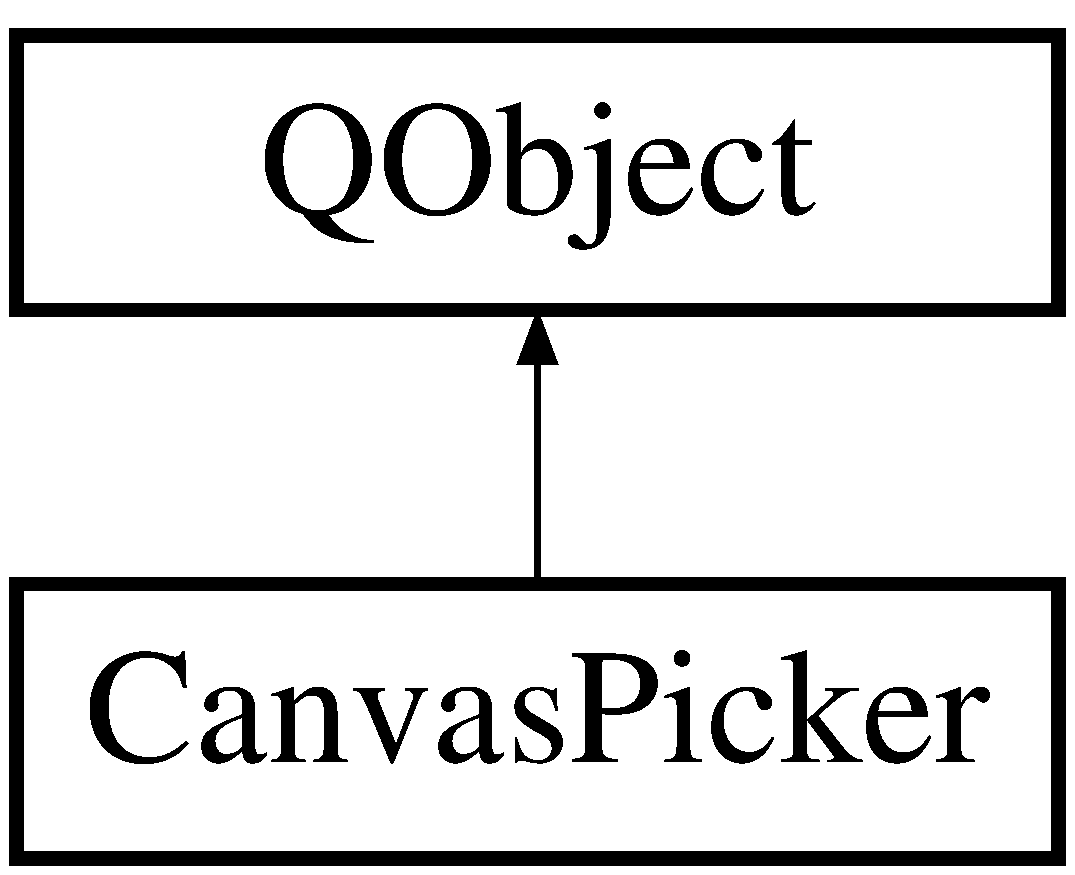
\includegraphics[height=2.000000cm]{classCanvasPicker}
\end{center}
\end{figure}
\subsection*{Public Member Functions}
\begin{DoxyCompactItemize}
\item 
\mbox{\Hypertarget{classCanvasPicker_a1f63183524af385cc42ef0f16a273a87}\label{classCanvasPicker_a1f63183524af385cc42ef0f16a273a87}} 
{\bfseries Canvas\+Picker} (Qwt\+Plot $\ast$plot)
\item 
\mbox{\Hypertarget{classCanvasPicker_a5214f5f57985d9a4c32ed4c97359da61}\label{classCanvasPicker_a5214f5f57985d9a4c32ed4c97359da61}} 
virtual bool {\bfseries event\+Filter} (Q\+Object $\ast$, Q\+Event $\ast$)
\item 
\mbox{\Hypertarget{classCanvasPicker_a270dbff23f04e8338d9e07b045b845d1}\label{classCanvasPicker_a270dbff23f04e8338d9e07b045b845d1}} 
virtual bool {\bfseries event} (Q\+Event $\ast$)
\end{DoxyCompactItemize}


The documentation for this class was generated from the following files\+:\begin{DoxyCompactItemize}
\item 
src/display\+\_\+buildblock/canvaspicker.\+h\item 
src/display\+\_\+buildblock/canvaspicker.\+cpp\end{DoxyCompactItemize}

\hypertarget{classViewer_1_1ColorMap}{}\section{Viewer\+:\+:Color\+Map Class Reference}
\label{classViewer_1_1ColorMap}\index{Viewer\+::\+Color\+Map@{Viewer\+::\+Color\+Map}}


Colormaps. Defaults at BW grayscale.  




{\ttfamily \#include $<$common.\+h$>$}

Inheritance diagram for Viewer\+:\+:Color\+Map\+:\begin{figure}[H]
\begin{center}
\leavevmode
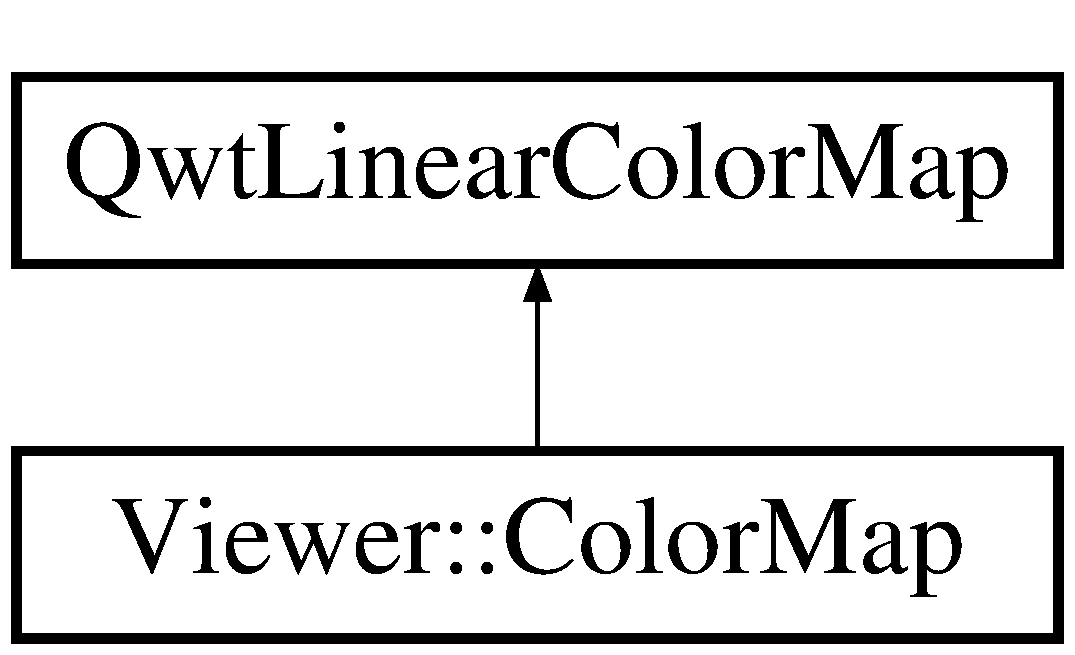
\includegraphics[height=2.000000cm]{classViewer_1_1ColorMap}
\end{center}
\end{figure}
\subsection*{Public Member Functions}
\begin{DoxyCompactItemize}
\item 
\mbox{\Hypertarget{classViewer_1_1ColorMap_a96bf84d0330588969e2dfd08312159d7}\label{classViewer_1_1ColorMap_a96bf84d0330588969e2dfd08312159d7}} 
void \mbox{\hyperlink{classViewer_1_1ColorMap_a96bf84d0330588969e2dfd08312159d7}{set\+Colormap}} (Q\+String name)
\begin{DoxyCompactList}\small\item\em Set the active \mbox{\hyperlink{classViewer_1_1ColorMap}{Color\+Map}} by name. \end{DoxyCompactList}\item 
\mbox{\Hypertarget{classViewer_1_1ColorMap_af5d66615f319e77c79fd6ed6a4df7ea4}\label{classViewer_1_1ColorMap_af5d66615f319e77c79fd6ed6a4df7ea4}} 
void \mbox{\hyperlink{classViewer_1_1ColorMap_af5d66615f319e77c79fd6ed6a4df7ea4}{set\+Colormap}} (int index)
\begin{DoxyCompactList}\small\item\em Set the active \mbox{\hyperlink{classViewer_1_1ColorMap}{Color\+Map}} by index. \end{DoxyCompactList}\item 
\mbox{\Hypertarget{classViewer_1_1ColorMap_a20586fb34a373264c9948ed70fb4f8c2}\label{classViewer_1_1ColorMap_a20586fb34a373264c9948ed70fb4f8c2}} 
void \mbox{\hyperlink{classViewer_1_1ColorMap_a20586fb34a373264c9948ed70fb4f8c2}{set\+\_\+\+BW}} ()
\begin{DoxyCompactList}\small\item\em Set Black -\/ White grayscale. \end{DoxyCompactList}\item 
\mbox{\Hypertarget{classViewer_1_1ColorMap_a73653a443aa595f23a48aa03c17e7071}\label{classViewer_1_1ColorMap_a73653a443aa595f23a48aa03c17e7071}} 
void \mbox{\hyperlink{classViewer_1_1ColorMap_a73653a443aa595f23a48aa03c17e7071}{set\+\_\+\+WB}} ()
\begin{DoxyCompactList}\small\item\em Set White -\/ Black grayscale. \end{DoxyCompactList}\item 
\mbox{\Hypertarget{classViewer_1_1ColorMap_a1f56d2420ac2c69688711c70ec3a201c}\label{classViewer_1_1ColorMap_a1f56d2420ac2c69688711c70ec3a201c}} 
void \mbox{\hyperlink{classViewer_1_1ColorMap_a1f56d2420ac2c69688711c70ec3a201c}{set\+\_\+\+J\+ET}} ()
\begin{DoxyCompactList}\small\item\em Set Jet, popular by old Matlab. \end{DoxyCompactList}\item 
\mbox{\Hypertarget{classViewer_1_1ColorMap_a8fc61d8156526f864be259cb532f9621}\label{classViewer_1_1ColorMap_a8fc61d8156526f864be259cb532f9621}} 
void \mbox{\hyperlink{classViewer_1_1ColorMap_a8fc61d8156526f864be259cb532f9621}{set\+\_\+qwt}} ()
\begin{DoxyCompactList}\small\item\em Set Q\+WT default \mbox{\hyperlink{classViewer_1_1ColorMap}{Color\+Map}}. \end{DoxyCompactList}\item 
\mbox{\Hypertarget{classViewer_1_1ColorMap_a59acb5dc0a0ffcbe0b188a0e1742d901}\label{classViewer_1_1ColorMap_a59acb5dc0a0ffcbe0b188a0e1742d901}} 
void \mbox{\hyperlink{classViewer_1_1ColorMap_a59acb5dc0a0ffcbe0b188a0e1742d901}{set\+\_\+\+Viridis}} ()
\begin{DoxyCompactList}\small\item\em Set Viridis \mbox{\hyperlink{classViewer_1_1ColorMap}{Color\+Map}}. \end{DoxyCompactList}\item 
\mbox{\Hypertarget{classViewer_1_1ColorMap_a3bc78d781d00be3fbe437505073f1a17}\label{classViewer_1_1ColorMap_a3bc78d781d00be3fbe437505073f1a17}} 
Q\+Color \mbox{\hyperlink{classViewer_1_1ColorMap_a3bc78d781d00be3fbe437505073f1a17}{get\+\_\+background}} () const
\begin{DoxyCompactList}\small\item\em Returns the first Color of the \mbox{\hyperlink{classViewer_1_1ColorMap}{Color\+Map}}. \end{DoxyCompactList}\item 
\mbox{\Hypertarget{classViewer_1_1ColorMap_a45f3fee7f63adbd3df53f9d6c7b5d148}\label{classViewer_1_1ColorMap_a45f3fee7f63adbd3df53f9d6c7b5d148}} 
Q\+Color \mbox{\hyperlink{classViewer_1_1ColorMap_a45f3fee7f63adbd3df53f9d6c7b5d148}{get\+\_\+peak\+\_\+color}} () const
\begin{DoxyCompactList}\small\item\em Returns the last Color of the \mbox{\hyperlink{classViewer_1_1ColorMap}{Color\+Map}}. \end{DoxyCompactList}\end{DoxyCompactItemize}
\subsection*{Static Public Member Functions}
\begin{DoxyCompactItemize}
\item 
\mbox{\Hypertarget{classViewer_1_1ColorMap_afa76c34f7d1b8388d25bf181743e2cc7}\label{classViewer_1_1ColorMap_afa76c34f7d1b8388d25bf181743e2cc7}} 
static Q\+String\+List \mbox{\hyperlink{classViewer_1_1ColorMap_afa76c34f7d1b8388d25bf181743e2cc7}{get\+Colormap\+List}} ()
\begin{DoxyCompactList}\small\item\em Get the list with all the available options. \end{DoxyCompactList}\end{DoxyCompactItemize}


\subsection{Detailed Description}
Colormaps. Defaults at BW grayscale. 

The documentation for this class was generated from the following file\+:\begin{DoxyCompactItemize}
\item 
src/buildblock/common.\+h\end{DoxyCompactItemize}

\hypertarget{classViewer_1_1CommonToAll}{}\section{Viewer\+:\+:Common\+To\+All Class Reference}
\label{classViewer_1_1CommonToAll}\index{Viewer\+::\+Common\+To\+All@{Viewer\+::\+Common\+To\+All}}


 




{\ttfamily \#include $<$common.\+h$>$}

Inheritance diagram for Viewer\+:\+:Common\+To\+All\+:\begin{figure}[H]
\begin{center}
\leavevmode
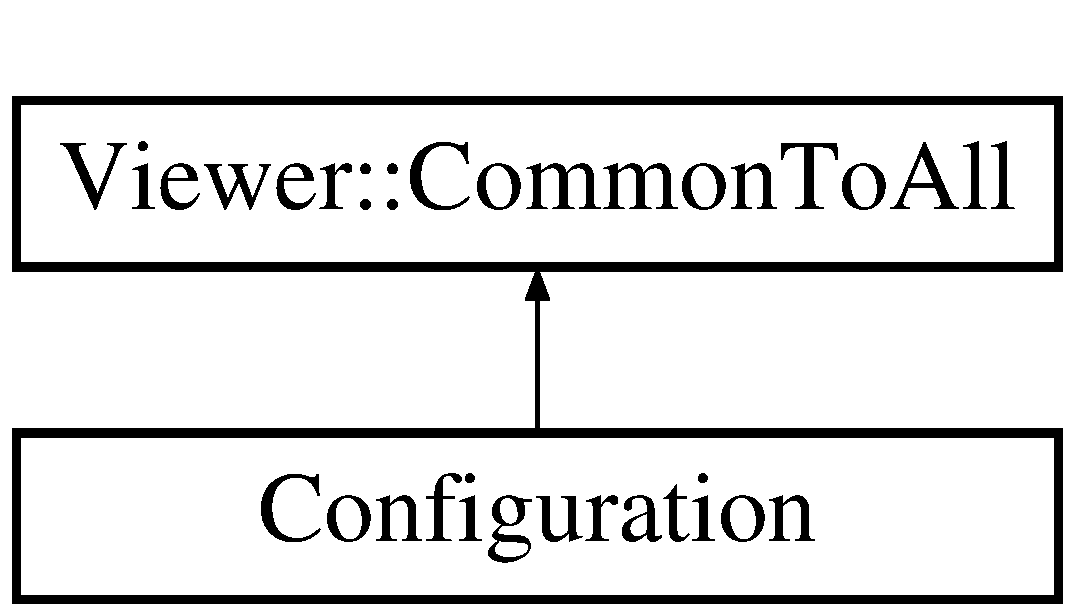
\includegraphics[height=2.000000cm]{classViewer_1_1CommonToAll}
\end{center}
\end{figure}
\subsection*{Public Attributes}
\begin{DoxyCompactItemize}
\item 
\mbox{\Hypertarget{classViewer_1_1CommonToAll_a6d05cfc549856952676aedd015e3b57b}\label{classViewer_1_1CommonToAll_a6d05cfc549856952676aedd015e3b57b}} 
Q\+Map$<$ qint8, Q\+String $>$ {\bfseries view\+Orders}
\end{DoxyCompactItemize}


\subsection{Detailed Description}


The documentation for this class was generated from the following file\+:\begin{DoxyCompactItemize}
\item 
src/buildblock/common.\+h\end{DoxyCompactItemize}

\hypertarget{classConfiguration}{}\section{Configuration Class Reference}
\label{classConfiguration}\index{Configuration@{Configuration}}
Inheritance diagram for Configuration\+:\begin{figure}[H]
\begin{center}
\leavevmode
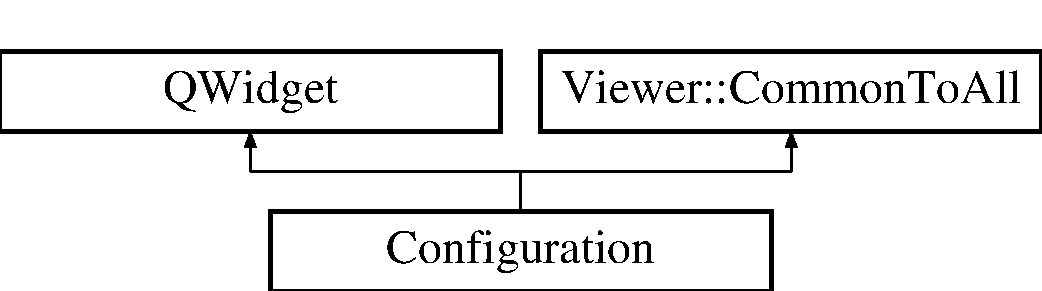
\includegraphics[height=2.000000cm]{classConfiguration}
\end{center}
\end{figure}
\subsection*{Public Member Functions}
\begin{DoxyCompactItemize}
\item 
\mbox{\Hypertarget{classConfiguration_a2e4474e9c5370084c1b24037b90b9557}\label{classConfiguration_a2e4474e9c5370084c1b24037b90b9557}} 
{\bfseries Configuration} (Q\+Widget $\ast$parent=nullptr)
\end{DoxyCompactItemize}
\subsection*{Public Attributes}
\begin{DoxyCompactItemize}
\item 
\mbox{\Hypertarget{classConfiguration_a6194decfd2dc5dbce1a8da67044c356a}\label{classConfiguration_a6194decfd2dc5dbce1a8da67044c356a}} 
qint8 {\bfseries cur\+Color\+Map\+\_\+index}
\item 
\mbox{\Hypertarget{classConfiguration_a28457f61f901ab5dabd7d47328ba4a34}\label{classConfiguration_a28457f61f901ab5dabd7d47328ba4a34}} 
qint8 {\bfseries num\+View\+Ports}
\item 
\mbox{\Hypertarget{classConfiguration_ac4fd650a5af1e2342e17d0c7ba3b25bf}\label{classConfiguration_ac4fd650a5af1e2342e17d0c7ba3b25bf}} 
bool {\bfseries show\+Histogram}
\item 
\mbox{\Hypertarget{classConfiguration_a4b9b95973c7ad8d078fded238961c82e}\label{classConfiguration_a4b9b95973c7ad8d078fded238961c82e}} 
qint8 {\bfseries n\+Bins}
\item 
\mbox{\Hypertarget{classConfiguration_a4a6f45e6f4c5f545bfbb3b084cc7e42b}\label{classConfiguration_a4a6f45e6f4c5f545bfbb3b084cc7e42b}} 
Orientation {\bfseries viewing\+\_\+orientation}
\item 
\mbox{\Hypertarget{classViewer_1_1CommonToAll_a6d05cfc549856952676aedd015e3b57b}\label{classViewer_1_1CommonToAll_a6d05cfc549856952676aedd015e3b57b}} 
Q\+Map$<$ qint8, Q\+String $>$ {\bfseries view\+Orders}
\end{DoxyCompactItemize}


The documentation for this class was generated from the following files\+:\begin{DoxyCompactItemize}
\item 
src/buildblock/configuration.\+h\item 
src/buildblock/configuration.\+cpp\end{DoxyCompactItemize}

\hypertarget{classContrastMan}{}\section{Contrast\+Man Class Reference}
\label{classContrastMan}\index{Contrast\+Man@{Contrast\+Man}}


The \mbox{\hyperlink{classContrastMan}{Contrast\+Man}} class The base widget for the display of the Contrast and WL operations.  




{\ttfamily \#include $<$contrastman.\+h$>$}

Inheritance diagram for Contrast\+Man\+:\begin{figure}[H]
\begin{center}
\leavevmode
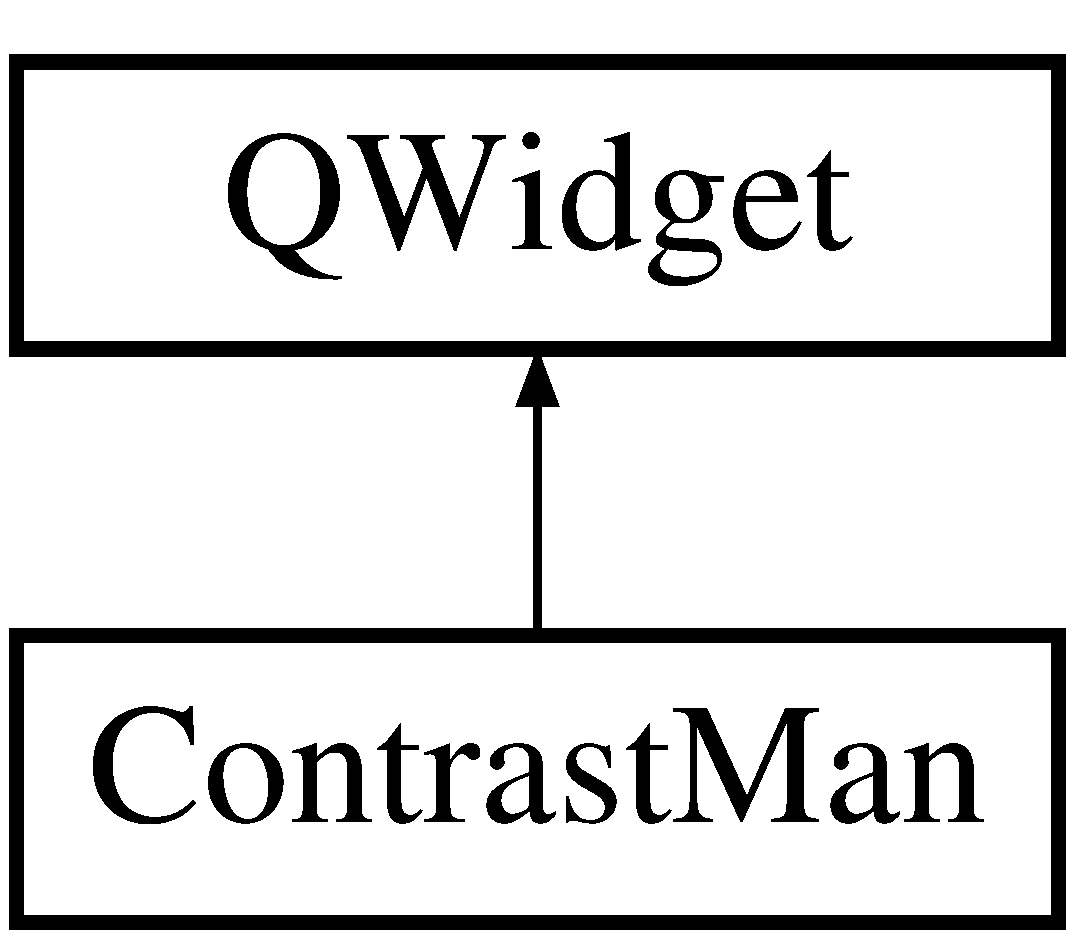
\includegraphics[height=2.000000cm]{classContrastMan}
\end{center}
\end{figure}
\subsection*{Public Member Functions}
\begin{DoxyCompactItemize}
\item 
\mbox{\Hypertarget{classContrastMan_acb952aac920f10c9eef753cb6d09ebf3}\label{classContrastMan_acb952aac920f10c9eef753cb6d09ebf3}} 
{\bfseries Contrast\+Man} (Q\+Widget $\ast$parent=0)
\item 
\mbox{\Hypertarget{classContrastMan_a253a84b069a8334d5c0f3b367f70e2cb}\label{classContrastMan_a253a84b069a8334d5c0f3b367f70e2cb}} 
void \mbox{\hyperlink{classContrastMan_a253a84b069a8334d5c0f3b367f70e2cb}{set\+Screen}} (\mbox{\hyperlink{classScreen__manager}{Screen\+\_\+manager}} $\ast$\+\_\+s)
\begin{DoxyCompactList}\small\item\em Set the \mbox{\hyperlink{classScreen__manager}{Screen\+\_\+manager}} for the operations. \end{DoxyCompactList}\item 
\mbox{\Hypertarget{classContrastMan_ab84677343dce962a03ec0e755c006f84}\label{classContrastMan_ab84677343dce962a03ec0e755c006f84}} 
void \mbox{\hyperlink{classContrastMan_ab84677343dce962a03ec0e755c006f84}{unset\+Screen}} ()
\begin{DoxyCompactList}\small\item\em Unset the current \mbox{\hyperlink{classScreen__manager}{Screen\+\_\+manager}}. \end{DoxyCompactList}\end{DoxyCompactItemize}
\subsection*{Protected Attributes}
\begin{DoxyCompactItemize}
\item 
\mbox{\Hypertarget{classContrastMan_ae9cdb0488404448a230e444c204ca79b}\label{classContrastMan_ae9cdb0488404448a230e444c204ca79b}} 
\mbox{\hyperlink{classScreen__manager}{Screen\+\_\+manager}} $\ast$ \mbox{\hyperlink{classContrastMan_ae9cdb0488404448a230e444c204ca79b}{sc}}
\begin{DoxyCompactList}\small\item\em Pointer to hold the current connected \mbox{\hyperlink{classScreen__manager}{Screen\+\_\+manager}}. \end{DoxyCompactList}\item 
\mbox{\Hypertarget{classContrastMan_a2d36ff4044963f35a1f9a1dc190b7b85}\label{classContrastMan_a2d36ff4044963f35a1f9a1dc190b7b85}} 
\mbox{\hyperlink{classBarScreenWL}{Bar\+Screen\+WL}} $\ast$ \mbox{\hyperlink{classContrastMan_a2d36ff4044963f35a1f9a1dc190b7b85}{my\+\_\+histogram}}
\begin{DoxyCompactList}\small\item\em Pointer to hold the \mbox{\hyperlink{classBarScreenWL}{Bar\+Screen\+WL}}. \end{DoxyCompactList}\end{DoxyCompactItemize}


\subsection{Detailed Description}
The \mbox{\hyperlink{classContrastMan}{Contrast\+Man}} class The base widget for the display of the Contrast and WL operations. 

The documentation for this class was generated from the following files\+:\begin{DoxyCompactItemize}
\item 
src/ui\+\_\+buildblock/contrastman.\+h\item 
src/ui\+\_\+buildblock/contrastman.\+cpp\end{DoxyCompactItemize}

\hypertarget{classCrossPointerTool}{}\section{Cross\+Pointer\+Tool Class Reference}
\label{classCrossPointerTool}\index{Cross\+Pointer\+Tool@{Cross\+Pointer\+Tool}}
Inheritance diagram for Cross\+Pointer\+Tool\+:\begin{figure}[H]
\begin{center}
\leavevmode
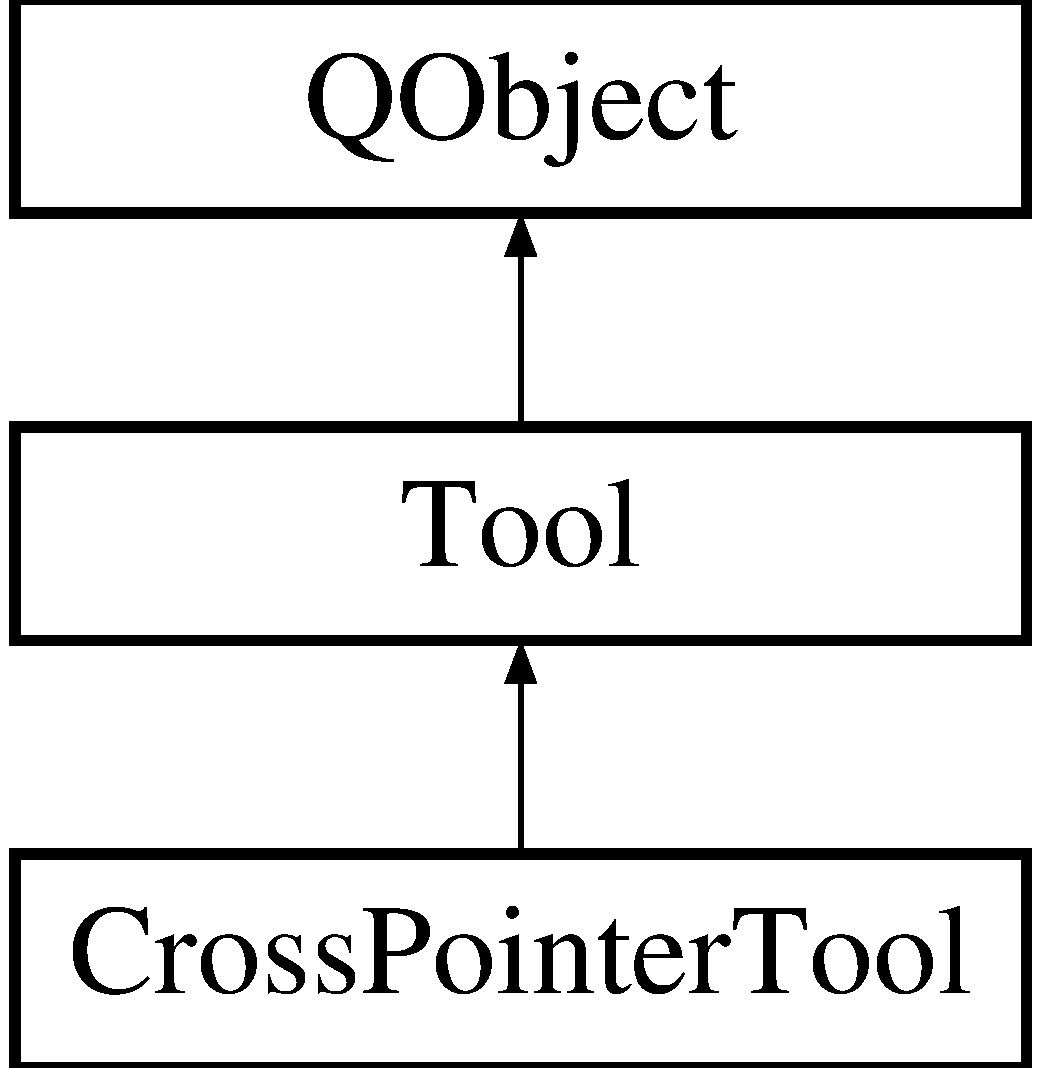
\includegraphics[height=3.000000cm]{classCrossPointerTool}
\end{center}
\end{figure}
\subsection*{Signals}
\begin{DoxyCompactItemize}
\item 
\mbox{\Hypertarget{classCrossPointerTool_ac59ee8dcb0892aeb22c6eef0316deb86}\label{classCrossPointerTool_ac59ee8dcb0892aeb22c6eef0316deb86}} 
void {\bfseries this\+\_\+location} (const Q\+Vector3D \&ps, const float \&v)
\item 
\mbox{\Hypertarget{classTool_a68dea3e4c911f3174176084d350865cc}\label{classTool_a68dea3e4c911f3174176084d350865cc}} 
void {\bfseries this\+\_\+selection} (const Q\+Vector$<$ Q\+PointF $>$ \&, Qwt\+Plot $\ast$)
\end{DoxyCompactItemize}
\subsection*{Public Member Functions}
\begin{DoxyCompactItemize}
\item 
\mbox{\Hypertarget{classCrossPointerTool_a5e59e97c427f36aa0d2554c1da37eccf}\label{classCrossPointerTool_a5e59e97c427f36aa0d2554c1da37eccf}} 
{\bfseries Cross\+Pointer\+Tool} (Q\+Widget $\ast$parent=0)
\item 
\mbox{\Hypertarget{classCrossPointerTool_ae2aadb3d5553c34805c9ec6f7f4fc854}\label{classCrossPointerTool_ae2aadb3d5553c34805c9ec6f7f4fc854}} 
virtual void {\bfseries finished\+Selecting} ()
\item 
virtual void \mbox{\hyperlink{classCrossPointerTool_a99e1b8f0669837dc5524c446e3dd401c}{clear\+Before\+Un\+Set}} ()
\item 
\mbox{\Hypertarget{classTool_a020bd5757a03ea7321848a3874f3a8cb}\label{classTool_a020bd5757a03ea7321848a3874f3a8cb}} 
virtual bool {\bfseries event\+Filter} (Q\+Object $\ast$, Q\+Event $\ast$)
\item 
\mbox{\Hypertarget{classTool_aa30c64915020a71d0ea8650e8e966336}\label{classTool_aa30c64915020a71d0ea8650e8e966336}} 
virtual Q\+String {\bfseries get\+\_\+name} () const
\item 
\mbox{\Hypertarget{classTool_a507adfcdafc818d9628b952001b93f3c}\label{classTool_a507adfcdafc818d9628b952001b93f3c}} 
void {\bfseries get\+\_\+data} (Q\+Vector$<$ Q\+PointF $>$ \&, Qwt\+Plot $\ast$)
\end{DoxyCompactItemize}
\subsection*{Protected Member Functions}
\begin{DoxyCompactItemize}
\item 
\mbox{\Hypertarget{classCrossPointerTool_a0b9aacf0090eee20cf1ba588db882be1}\label{classCrossPointerTool_a0b9aacf0090eee20cf1ba588db882be1}} 
void \mbox{\hyperlink{classCrossPointerTool_a0b9aacf0090eee20cf1ba588db882be1}{select}} (const Q\+PointF \&ps)
\begin{DoxyCompactList}\small\item\em On mouse press action. \end{DoxyCompactList}\item 
\mbox{\Hypertarget{classCrossPointerTool_ad90be83c2f2b4a2ae276974adb1ce157}\label{classCrossPointerTool_ad90be83c2f2b4a2ae276974adb1ce157}} 
void \mbox{\hyperlink{classCrossPointerTool_ad90be83c2f2b4a2ae276974adb1ce157}{move}} (const Q\+PointF \&)
\begin{DoxyCompactList}\small\item\em On mouse press and drag action. \end{DoxyCompactList}\item 
\mbox{\Hypertarget{classCrossPointerTool_a736f76da2473660084ea5ecc2fd313c1}\label{classCrossPointerTool_a736f76da2473660084ea5ecc2fd313c1}} 
void \mbox{\hyperlink{classCrossPointerTool_a736f76da2473660084ea5ecc2fd313c1}{clear\+Selection}} ()
\begin{DoxyCompactList}\small\item\em Remove all curves from the c\+\_\+paint\+Device. \end{DoxyCompactList}\item 
bool \mbox{\hyperlink{classTool_a81244366dc1b9f55465ed6f37b81033c}{check\+Point\+In\+Range}} (const Q\+PointF \&\+\_\+local)
\end{DoxyCompactItemize}
\subsection*{Protected Attributes}
\begin{DoxyCompactItemize}
\item 
\mbox{\Hypertarget{classCrossPointerTool_a461e7131fedd8d680870fb2f9a0a58a6}\label{classCrossPointerTool_a461e7131fedd8d680870fb2f9a0a58a6}} 
Qwt\+Plot\+Curve $\ast$ {\bfseries curveA}
\item 
\mbox{\Hypertarget{classCrossPointerTool_aadcce371c379f5fccf1bf43d59e22765}\label{classCrossPointerTool_aadcce371c379f5fccf1bf43d59e22765}} 
Qwt\+Plot\+Curve $\ast$ {\bfseries curveB}
\item 
\mbox{\Hypertarget{classTool_af0935d8e8edd73d8ec85424b5b15196b}\label{classTool_af0935d8e8edd73d8ec85424b5b15196b}} 
Q\+String {\bfseries name}
\item 
\mbox{\Hypertarget{classTool_a1e301a03c5806c900786760d80049380}\label{classTool_a1e301a03c5806c900786760d80049380}} 
Qwt\+Plot\+Canvas $\ast$ {\bfseries c\+\_\+paint\+Device}
\item 
\mbox{\Hypertarget{classTool_af1d11cc5374ba7eb7c1d41cfb5d4e981}\label{classTool_af1d11cc5374ba7eb7c1d41cfb5d4e981}} 
Qwt\+Plot\+Spectrogram $\ast$ {\bfseries d\+\_\+spectrogram}
\item 
Q\+Vector$<$ Q\+PointF $>$ \mbox{\hyperlink{classTool_a68be77a2e364a7b13d7206388ba5843e}{\+\_\+points}}
\end{DoxyCompactItemize}


\subsection{Member Function Documentation}
\mbox{\Hypertarget{classTool_a81244366dc1b9f55465ed6f37b81033c}\label{classTool_a81244366dc1b9f55465ed6f37b81033c}} 
\index{Cross\+Pointer\+Tool@{Cross\+Pointer\+Tool}!check\+Point\+In\+Range@{check\+Point\+In\+Range}}
\index{check\+Point\+In\+Range@{check\+Point\+In\+Range}!Cross\+Pointer\+Tool@{Cross\+Pointer\+Tool}}
\subsubsection{\texorpdfstring{check\+Point\+In\+Range()}{checkPointInRange()}}
{\footnotesize\ttfamily bool Tool\+::check\+Point\+In\+Range (\begin{DoxyParamCaption}\item[{const Q\+PointF \&}]{\+\_\+local }\end{DoxyParamCaption})\hspace{0.3cm}{\ttfamily [protected]}, {\ttfamily [inherited]}}

This is a preliminiry check to see if the point is within the axis range. It has been proven somewhat week condition, as in many cases it fails to provide realible results. \mbox{\Hypertarget{classCrossPointerTool_a99e1b8f0669837dc5524c446e3dd401c}\label{classCrossPointerTool_a99e1b8f0669837dc5524c446e3dd401c}} 
\index{Cross\+Pointer\+Tool@{Cross\+Pointer\+Tool}!clear\+Before\+Un\+Set@{clear\+Before\+Un\+Set}}
\index{clear\+Before\+Un\+Set@{clear\+Before\+Un\+Set}!Cross\+Pointer\+Tool@{Cross\+Pointer\+Tool}}
\subsubsection{\texorpdfstring{clear\+Before\+Un\+Set()}{clearBeforeUnSet()}}
{\footnotesize\ttfamily void Cross\+Pointer\+Tool\+::clear\+Before\+Un\+Set (\begin{DoxyParamCaption}{ }\end{DoxyParamCaption})\hspace{0.3cm}{\ttfamily [virtual]}}

Cal this function to clean before unsetting a tool. It will try to tight up the screen. 

Implements \mbox{\hyperlink{classTool_a7d9e7d03f4a34d71850cbbfc16ca8532}{Tool}}.



\subsection{Member Data Documentation}
\mbox{\Hypertarget{classTool_a68be77a2e364a7b13d7206388ba5843e}\label{classTool_a68be77a2e364a7b13d7206388ba5843e}} 
\index{Cross\+Pointer\+Tool@{Cross\+Pointer\+Tool}!\+\_\+points@{\+\_\+points}}
\index{\+\_\+points@{\+\_\+points}!Cross\+Pointer\+Tool@{Cross\+Pointer\+Tool}}
\subsubsection{\texorpdfstring{\+\_\+points}{\_points}}
{\footnotesize\ttfamily Q\+Vector$<$Q\+PointF$>$ Tool\+::\+\_\+points\hspace{0.3cm}{\ttfamily [protected]}, {\ttfamily [inherited]}}

This vector holds the characteristic points of the selected R\+OI. The \mbox{\hyperlink{classCrossPointerTool}{Cross\+Pointer\+Tool}} has just one point. The \mbox{\hyperlink{classLineTool}{Line\+Tool}} has two points (e.\+g. start and stop) e.\+t.\+c 

The documentation for this class was generated from the following files\+:\begin{DoxyCompactItemize}
\item 
src/tools\+\_\+buildblock/pointercrosstool.\+h\item 
src/tools\+\_\+buildblock/pointercrosstool.\+cpp\end{DoxyCompactItemize}

\hypertarget{classdataSeries}{}\section{data\+Series Class Reference}
\label{classdataSeries}\index{data\+Series@{data\+Series}}


The documentation for this class was generated from the following files\+:\begin{DoxyCompactItemize}
\item 
src/buildblock/dataseries.\+h\item 
src/buildblock/dataseries.\+cpp\end{DoxyCompactItemize}

\hypertarget{classDialog}{}\section{Dialog Class Reference}
\label{classDialog}\index{Dialog@{Dialog}}


The \mbox{\hyperlink{classDialog}{Dialog}} class This a dialog about the view orientation. But in the future it might become a more generic dialog box.  




{\ttfamily \#include $<$dialog.\+h$>$}

Inheritance diagram for Dialog\+:\begin{figure}[H]
\begin{center}
\leavevmode
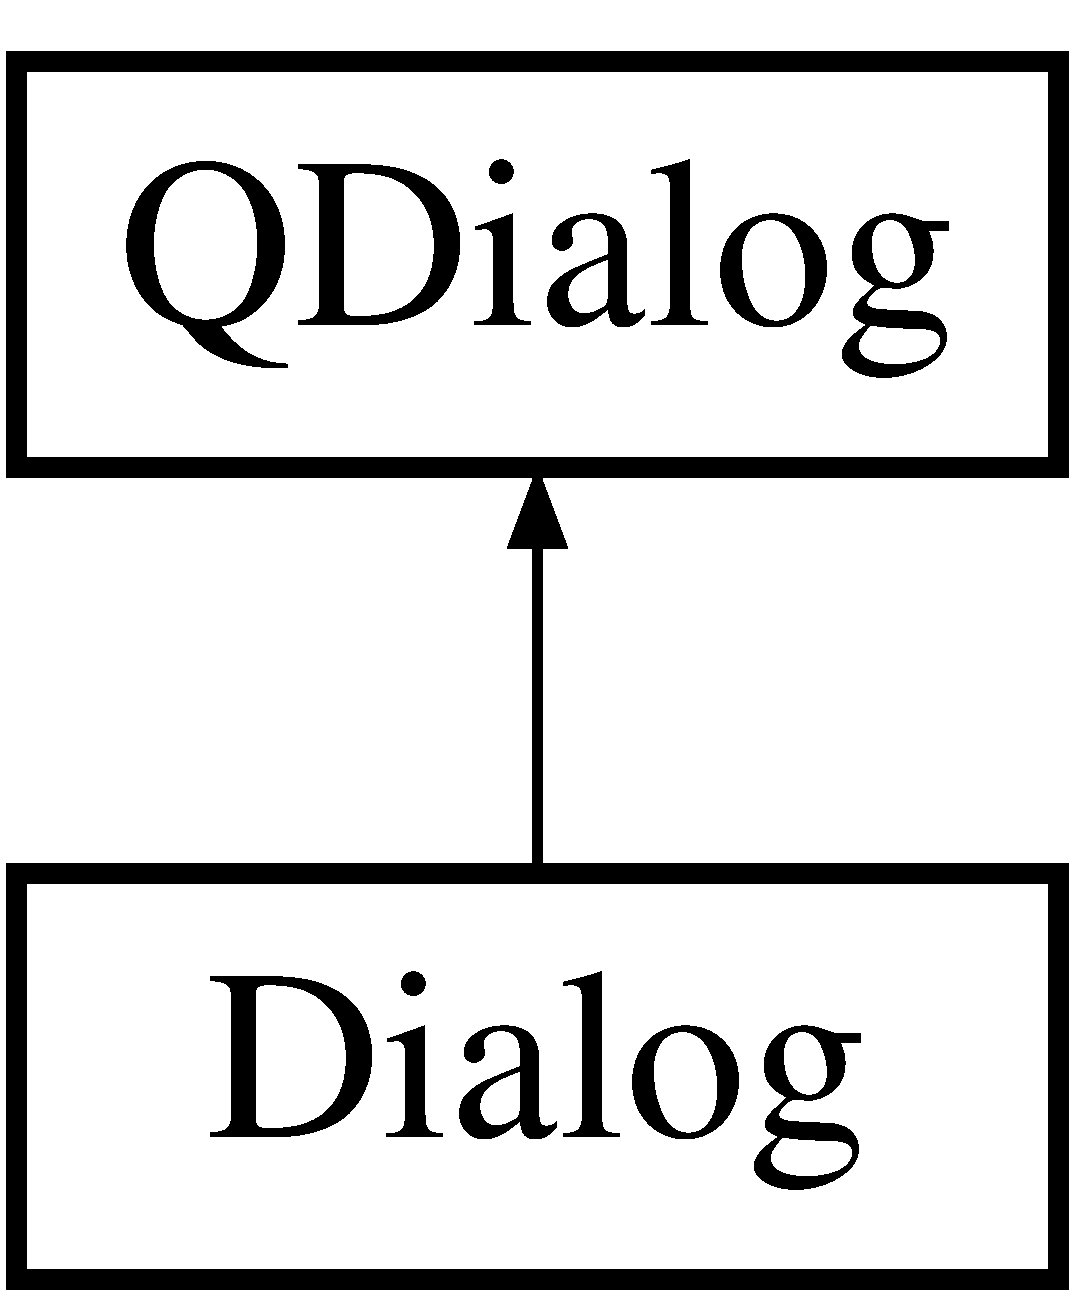
\includegraphics[height=2.000000cm]{classDialog}
\end{center}
\end{figure}
\subsection*{Public Member Functions}
\begin{DoxyCompactItemize}
\item 
\mbox{\Hypertarget{classDialog_a20eb290a76ed7ab7a96822527a061cbf}\label{classDialog_a20eb290a76ed7ab7a96822527a061cbf}} 
{\bfseries Dialog} (Q\+String space, Q\+Widget $\ast$parent=0)
\end{DoxyCompactItemize}
\subsection*{Public Attributes}
\begin{DoxyCompactItemize}
\item 
\mbox{\Hypertarget{classDialog_a1a1877cbe1d70bf773883ee26f3f3f77}\label{classDialog_a1a1877cbe1d70bf773883ee26f3f3f77}} 
int {\bfseries ret}
\item 
\mbox{\Hypertarget{classDialog_a23bf556d60e1249dae5dff6c7696ed18}\label{classDialog_a23bf556d60e1249dae5dff6c7696ed18}} 
Q\+Check\+Box $\ast$ {\bfseries chk\+Box}
\end{DoxyCompactItemize}


\subsection{Detailed Description}
The \mbox{\hyperlink{classDialog}{Dialog}} class This a dialog about the view orientation. But in the future it might become a more generic dialog box. 

The documentation for this class was generated from the following files\+:\begin{DoxyCompactItemize}
\item 
src/buildblock/dialog.\+h\item 
src/buildblock/dialog.\+cpp\end{DoxyCompactItemize}

\hypertarget{classdisplay__screen}{}\section{display\+\_\+screen Class Reference}
\label{classdisplay__screen}\index{display\+\_\+screen@{display\+\_\+screen}}
Inheritance diagram for display\+\_\+screen\+:\begin{figure}[H]
\begin{center}
\leavevmode
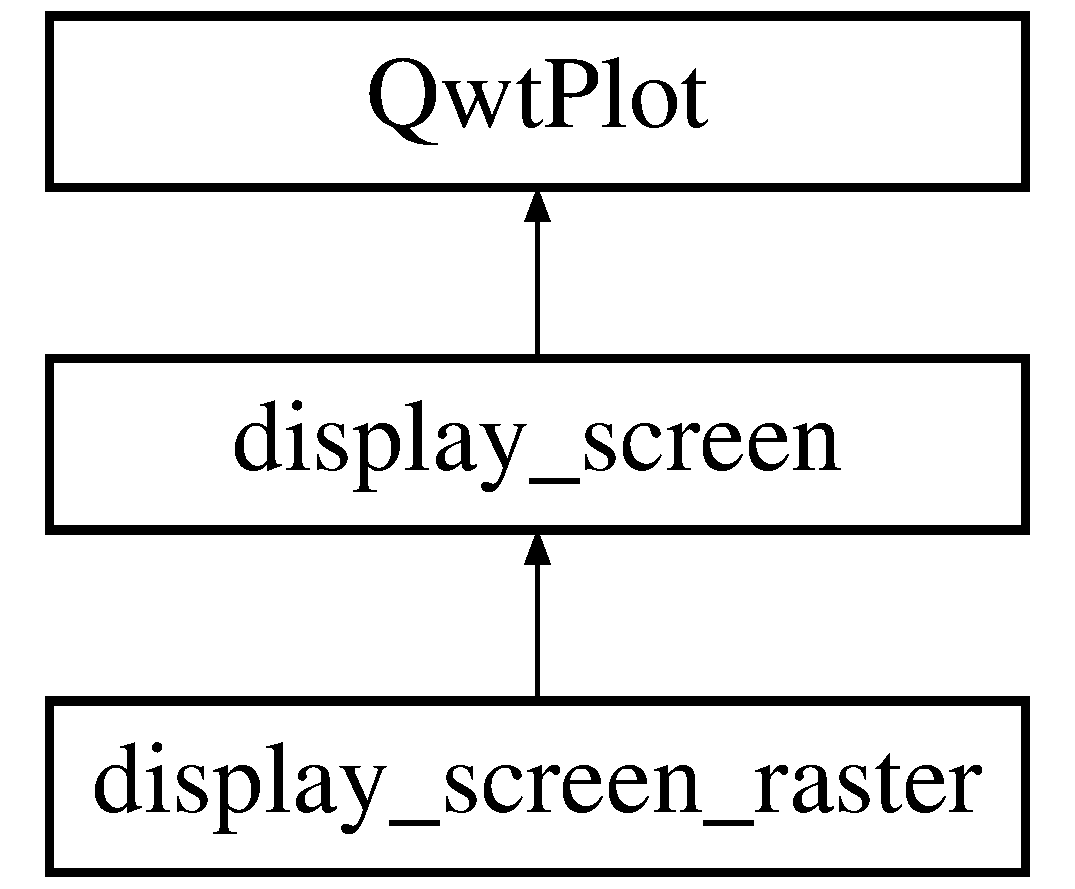
\includegraphics[height=3.000000cm]{classdisplay__screen}
\end{center}
\end{figure}
\subsection*{Signals}
\begin{DoxyCompactItemize}
\item 
\mbox{\Hypertarget{classdisplay__screen_ac606cfb3c58cd90b354c1b6997737074}\label{classdisplay__screen_ac606cfb3c58cd90b354c1b6997737074}} 
void {\bfseries activate\+Screen} (const qint32 \&)
\end{DoxyCompactItemize}
\subsection*{Public Member Functions}
\begin{DoxyCompactItemize}
\item 
\mbox{\Hypertarget{classdisplay__screen_a030b7a4cfc31bf2229ad29dd2301b0e3}\label{classdisplay__screen_a030b7a4cfc31bf2229ad29dd2301b0e3}} 
{\bfseries display\+\_\+screen} (Q\+Widget $\ast$parent=0)
\item 
\mbox{\Hypertarget{classdisplay__screen_a8e55d078385c987e8720037361ef604e}\label{classdisplay__screen_a8e55d078385c987e8720037361ef604e}} 
virtual void {\bfseries replot\+\_\+me} ()=0
\item 
\mbox{\Hypertarget{classdisplay__screen_a27d55d66129e2f3b99314c73d5457eaf}\label{classdisplay__screen_a27d55d66129e2f3b99314c73d5457eaf}} 
int {\bfseries get\+\_\+data\+\_\+size} ()
\item 
\mbox{\Hypertarget{classdisplay__screen_a1c77889dda840e1c37fc89d9a36b6931}\label{classdisplay__screen_a1c77889dda840e1c37fc89d9a36b6931}} 
virtual void {\bfseries set\+O\+CD} (const Q\+String \&\+\_\+l, const Q\+String \&\+\_\+r, const Q\+String \&\+\_\+t, const Q\+String \&\+\_\+b)=0
\item 
\mbox{\Hypertarget{classdisplay__screen_ac21347fc9744e48f10d498a6eb784358}\label{classdisplay__screen_ac21347fc9744e48f10d498a6eb784358}} 
virtual void {\bfseries set\+My\+Title} (const qint32 \&\+\_\+label)=0
\item 
\mbox{\Hypertarget{classdisplay__screen_a85b97edfde46cbe8136877c35bb6876d}\label{classdisplay__screen_a85b97edfde46cbe8136877c35bb6876d}} 
void \mbox{\hyperlink{classdisplay__screen_a85b97edfde46cbe8136877c35bb6876d}{clear\+Curves}} ()
\begin{DoxyCompactList}\small\item\em Remove every curve is on the screen. \end{DoxyCompactList}\item 
virtual void \mbox{\hyperlink{classdisplay__screen_aedda58c57969f054fb9bedd1ed01b62c}{clear\+Cursors}} ()=0
\item 
\mbox{\Hypertarget{classdisplay__screen_ac2ef804e167c1ba941dcf91134bbe769}\label{classdisplay__screen_ac2ef804e167c1ba941dcf91134bbe769}} 
void {\bfseries set\+\_\+active} (bool state)
\item 
\mbox{\Hypertarget{classdisplay__screen_ac64b0a65402d794e135c6c6e189d02a6}\label{classdisplay__screen_ac64b0a65402d794e135c6c6e189d02a6}} 
virtual void {\bfseries mouse\+Press\+Event} (Q\+Mouse\+Event $\ast$event)
\item 
\mbox{\Hypertarget{classdisplay__screen_aa422fde3414884615abd635e073bc737}\label{classdisplay__screen_aa422fde3414884615abd635e073bc737}} 
virtual void {\bfseries key\+Press\+Event} (Q\+Key\+Event $\ast$event)
\item 
\mbox{\Hypertarget{classdisplay__screen_ab54ec0811e324d192a75b3e538c66513}\label{classdisplay__screen_ab54ec0811e324d192a75b3e538c66513}} 
void {\bfseries set\+Address\+At\+Parent} (const qint32 \&id)
\item 
\mbox{\Hypertarget{classdisplay__screen_ab2a10597339ba6fb2de1744561158391}\label{classdisplay__screen_ab2a10597339ba6fb2de1744561158391}} 
virtual void {\bfseries set\+Interval} (const double \&\+\_\+min, const double \&\+\_\+max)=0
\item 
\mbox{\Hypertarget{classdisplay__screen_a59e371ef5f03f966706cf0d33331f2c6}\label{classdisplay__screen_a59e371ef5f03f966706cf0d33331f2c6}} 
virtual Q\+Vector$<$ double $>$\+::Const\+Iterator {\bfseries get\+\_\+data\+\_\+const\+\_\+begin} () const =0
\item 
\mbox{\Hypertarget{classdisplay__screen_a7746c54dcbb593f8c328d5318d686256}\label{classdisplay__screen_a7746c54dcbb593f8c328d5318d686256}} 
virtual Q\+Vector$<$ double $>$\+::Const\+Iterator {\bfseries get\+\_\+data\+\_\+const\+\_\+end} () const =0
\item 
\mbox{\Hypertarget{classdisplay__screen_a1a0a574c59e0c4cfd8ad8de4bb8e105d}\label{classdisplay__screen_a1a0a574c59e0c4cfd8ad8de4bb8e105d}} 
const double $\ast$ {\bfseries get\+\_\+max\+\_\+vis\+\_\+value\+\_\+ptr} () const
\item 
\mbox{\Hypertarget{classdisplay__screen_a8e8a2009db3859562e3d52e44731dd03}\label{classdisplay__screen_a8e8a2009db3859562e3d52e44731dd03}} 
const double $\ast$ {\bfseries get\+\_\+min\+\_\+vis\+\_\+value\+\_\+ptr} () const
\item 
\mbox{\Hypertarget{classdisplay__screen_ab6ae4f9a9b41b89976fc2742db40d431}\label{classdisplay__screen_ab6ae4f9a9b41b89976fc2742db40d431}} 
virtual void {\bfseries draw\+Cursor} (const bool \&\+\_\+s, const \mbox{\hyperlink{classViewer_1_1SimpleVector2D}{Viewer\+::\+Simple\+Vector2D}}$<$ int $>$ \&ps)=0
\item 
\mbox{\Hypertarget{classdisplay__screen_a6fecd6139a092ed9ee2a877a9e2b2fd3}\label{classdisplay__screen_a6fecd6139a092ed9ee2a877a9e2b2fd3}} 
virtual \mbox{\hyperlink{classViewer_1_1SimpleVector2D}{Viewer\+::\+Simple\+Vector2D}}$<$ int $>$ {\bfseries draw\+Cursor} (const bool \&\+\_\+s, const Q\+PointF \&ps)=0
\item 
\mbox{\Hypertarget{classdisplay__screen_a8bef78ebe05dc6e7174b07dc41ba8e4c}\label{classdisplay__screen_a8bef78ebe05dc6e7174b07dc41ba8e4c}} 
virtual void {\bfseries xy\+From\+Cell} (const \mbox{\hyperlink{classViewer_1_1SimpleVector2D}{Viewer\+::\+Simple\+Vector2D}}$<$ int $>$ \&, Q\+PointF \&)=0
\item 
\mbox{\Hypertarget{classdisplay__screen_aeb43714b249ecf4bb5693e6551298d57}\label{classdisplay__screen_aeb43714b249ecf4bb5693e6551298d57}} 
virtual void {\bfseries cell\+From\+XY} (const Q\+PointF \&\+\_\+p, \mbox{\hyperlink{classViewer_1_1SimpleVector2D}{Viewer\+::\+Simple\+Vector2D}}$<$ int $>$ \&\+\_\+v)=0
\item 
virtual void \mbox{\hyperlink{classdisplay__screen_a2788f315d8f91b4c8a2b870698ce6623}{write\+Values\+In\+Data}} (const stir\+::\+Proj\+Matrix\+Elems\+For\+One\+Bin \&, const float \&)=0
\item 
\mbox{\Hypertarget{classdisplay__screen_a17b159563b62a3c8bfd7245453ba421a}\label{classdisplay__screen_a17b159563b62a3c8bfd7245453ba421a}} 
void {\bfseries apply\+Function} (\mbox{\hyperlink{classWorker}{Worker}} $\ast$\+\_\+w)
\item 
\mbox{\Hypertarget{classdisplay__screen_a2df277a3abd63d90ec1ead11d0eb3818}\label{classdisplay__screen_a2df277a3abd63d90ec1ead11d0eb3818}} 
void {\bfseries remove\+Function} ()
\item 
\mbox{\Hypertarget{classdisplay__screen_addb4faa7ad8c8dd34de9543a01ecd4af}\label{classdisplay__screen_addb4faa7ad8c8dd34de9543a01ecd4af}} 
virtual stir\+::\+Cartesian\+Coordinate3D$<$ float $>$ \mbox{\hyperlink{classdisplay__screen_addb4faa7ad8c8dd34de9543a01ecd4af}{get\+Grid\+Spacing}} ()=0
\begin{DoxyCompactList}\small\item\em Return the Pixel hint (or grid spacing of the data) \end{DoxyCompactList}\end{DoxyCompactItemize}
\subsection*{Protected Slots}
\begin{DoxyCompactItemize}
\item 
\mbox{\Hypertarget{classdisplay__screen_a6312d4f51441872e8d9a677b5ae7584d}\label{classdisplay__screen_a6312d4f51441872e8d9a677b5ae7584d}} 
virtual void {\bfseries pop\+Up\+Menu} (const Q\+Point \&pos)
\end{DoxyCompactItemize}
\subsection*{Protected Member Functions}
\begin{DoxyCompactItemize}
\item 
\mbox{\Hypertarget{classdisplay__screen_a5f27a1aa1d1ef02823cdf23a686e5593}\label{classdisplay__screen_a5f27a1aa1d1ef02823cdf23a686e5593}} 
void \mbox{\hyperlink{classdisplay__screen_a5f27a1aa1d1ef02823cdf23a686e5593}{draw\+Selection\+Frame}} (bool state)
\begin{DoxyCompactList}\small\item\em Draw a frame around the display to indicate that this is the active. \end{DoxyCompactList}\end{DoxyCompactItemize}
\subsection*{Protected Attributes}
\begin{DoxyCompactItemize}
\item 
\mbox{\Hypertarget{classdisplay__screen_a52bf41a53070ae85bdf46ee75dd84f0d}\label{classdisplay__screen_a52bf41a53070ae85bdf46ee75dd84f0d}} 
Q\+Vector$<$ double $>$ \mbox{\hyperlink{classdisplay__screen_a52bf41a53070ae85bdf46ee75dd84f0d}{my\+\_\+data}}
\begin{DoxyCompactList}\small\item\em The data which are displayed on screen. \end{DoxyCompactList}\item 
\mbox{\Hypertarget{classdisplay__screen_a404e8f942e20b528e8017f693eea5ea5}\label{classdisplay__screen_a404e8f942e20b528e8017f693eea5ea5}} 
qint32 {\bfseries my\+Address}
\item 
\mbox{\Hypertarget{classdisplay__screen_aa5d0a895e06f256254d60c9a6761353a}\label{classdisplay__screen_aa5d0a895e06f256254d60c9a6761353a}} 
qint32 \mbox{\hyperlink{classdisplay__screen_aa5d0a895e06f256254d60c9a6761353a}{my\+\_\+label}}
\begin{DoxyCompactList}\small\item\em The number displayed at the bottom right corner. In sync with the scroll bar. \end{DoxyCompactList}\item 
\mbox{\Hypertarget{classdisplay__screen_aa36da095bb12f0f4c9a5063fc9477bf8}\label{classdisplay__screen_aa36da095bb12f0f4c9a5063fc9477bf8}} 
int {\bfseries size}
\item 
\mbox{\Hypertarget{classdisplay__screen_aefb44f5edee20d8ec3f1e6f1cb790db4}\label{classdisplay__screen_aefb44f5edee20d8ec3f1e6f1cb790db4}} 
bool {\bfseries cursor\+Status}
\item 
\mbox{\Hypertarget{classdisplay__screen_a456d4c817042e690b69f978fdbf16320}\label{classdisplay__screen_a456d4c817042e690b69f978fdbf16320}} 
Qwt\+Plot\+Text\+Label $\ast$ {\bfseries title\+Item}
\item 
\mbox{\Hypertarget{classdisplay__screen_ae6764a9d2d77f51e93cdc34ab277d48a}\label{classdisplay__screen_ae6764a9d2d77f51e93cdc34ab277d48a}} 
Qwt\+Plot\+Text\+Label $\ast$ {\bfseries l\+O\+C\+D\+Item}
\item 
\mbox{\Hypertarget{classdisplay__screen_a69d982deaa57cd6d447b7408093568a6}\label{classdisplay__screen_a69d982deaa57cd6d447b7408093568a6}} 
Qwt\+Plot\+Text\+Label $\ast$ {\bfseries r\+O\+C\+D\+Item}
\item 
\mbox{\Hypertarget{classdisplay__screen_a570edfafbba0d70fce7d9967958310aa}\label{classdisplay__screen_a570edfafbba0d70fce7d9967958310aa}} 
Qwt\+Plot\+Text\+Label $\ast$ {\bfseries b\+O\+C\+D\+Item}
\item 
\mbox{\Hypertarget{classdisplay__screen_a8faeeea1ba78a88dae699c43fa0ae087}\label{classdisplay__screen_a8faeeea1ba78a88dae699c43fa0ae087}} 
Qwt\+Plot\+Text\+Label $\ast$ {\bfseries t\+O\+C\+D\+Item}
\item 
\mbox{\Hypertarget{classdisplay__screen_a7babe15db1f589f15bb94c6f54a7c9fb}\label{classdisplay__screen_a7babe15db1f589f15bb94c6f54a7c9fb}} 
Q\+Font \mbox{\hyperlink{classdisplay__screen_a7babe15db1f589f15bb94c6f54a7c9fb}{font}}
\begin{DoxyCompactList}\small\item\em The font used for the O\+CD text. \end{DoxyCompactList}\item 
\mbox{\Hypertarget{classdisplay__screen_ad22570d6a6e8ed9b46f9040406ad812c}\label{classdisplay__screen_ad22570d6a6e8ed9b46f9040406ad812c}} 
Qwt\+Text \mbox{\hyperlink{classdisplay__screen_ad22570d6a6e8ed9b46f9040406ad812c}{title}}
\begin{DoxyCompactList}\small\item\em Text for the O\+CD texts. \end{DoxyCompactList}\item 
\mbox{\Hypertarget{classdisplay__screen_a8cd4a91142663ac54195431d5cd60e9d}\label{classdisplay__screen_a8cd4a91142663ac54195431d5cd60e9d}} 
Qwt\+Text {\bfseries l\+O\+CD}
\item 
\mbox{\Hypertarget{classdisplay__screen_aa622bfa993c2bec08e31f78b91fd4d2b}\label{classdisplay__screen_aa622bfa993c2bec08e31f78b91fd4d2b}} 
Qwt\+Text {\bfseries r\+O\+CD}
\item 
\mbox{\Hypertarget{classdisplay__screen_a050d88f65c01662ab2b637bfa90c7abd}\label{classdisplay__screen_a050d88f65c01662ab2b637bfa90c7abd}} 
Qwt\+Text {\bfseries b\+O\+CD}
\item 
\mbox{\Hypertarget{classdisplay__screen_a099a94fac1e3c0bab6884c8953a43031}\label{classdisplay__screen_a099a94fac1e3c0bab6884c8953a43031}} 
Qwt\+Text {\bfseries t\+O\+CD}
\item 
\mbox{\Hypertarget{classdisplay__screen_a7ffb415729f7d3d10505ac04f829582c}\label{classdisplay__screen_a7ffb415729f7d3d10505ac04f829582c}} 
double \mbox{\hyperlink{classdisplay__screen_a7ffb415729f7d3d10505ac04f829582c}{max\+\_\+value}}
\begin{DoxyCompactList}\small\item\em Max value of the display data. \end{DoxyCompactList}\item 
\mbox{\Hypertarget{classdisplay__screen_a3091e35b28219274fe9ffd8e8dc68c40}\label{classdisplay__screen_a3091e35b28219274fe9ffd8e8dc68c40}} 
double \mbox{\hyperlink{classdisplay__screen_a3091e35b28219274fe9ffd8e8dc68c40}{min\+\_\+value}}
\begin{DoxyCompactList}\small\item\em Min value of the display data. \end{DoxyCompactList}\item 
\mbox{\Hypertarget{classdisplay__screen_a0a040ebfadeba044ee2d887c43b37425}\label{classdisplay__screen_a0a040ebfadeba044ee2d887c43b37425}} 
double \mbox{\hyperlink{classdisplay__screen_a0a040ebfadeba044ee2d887c43b37425}{vis\+\_\+min}}
\begin{DoxyCompactList}\small\item\em Apparent min value -\/ W\&L operations set this value. \end{DoxyCompactList}\item 
\mbox{\Hypertarget{classdisplay__screen_a100a772813944bb4a41feab579ae11d8}\label{classdisplay__screen_a100a772813944bb4a41feab579ae11d8}} 
double \mbox{\hyperlink{classdisplay__screen_a100a772813944bb4a41feab579ae11d8}{vis\+\_\+max}}
\begin{DoxyCompactList}\small\item\em Apparent max value -\/ W\&L operations set this value. \end{DoxyCompactList}\item 
\mbox{\hyperlink{classWorker}{Worker}} $\ast$ \mbox{\hyperlink{classdisplay__screen_a54ed0638f240e4a044d9d4376233ec71}{filter}}
\end{DoxyCompactItemize}


\subsection{Member Function Documentation}
\mbox{\Hypertarget{classdisplay__screen_aedda58c57969f054fb9bedd1ed01b62c}\label{classdisplay__screen_aedda58c57969f054fb9bedd1ed01b62c}} 
\index{display\+\_\+screen@{display\+\_\+screen}!clear\+Cursors@{clear\+Cursors}}
\index{clear\+Cursors@{clear\+Cursors}!display\+\_\+screen@{display\+\_\+screen}}
\subsubsection{\texorpdfstring{clear\+Cursors()}{clearCursors()}}
{\footnotesize\ttfamily void display\+\_\+screen\+::clear\+Cursors (\begin{DoxyParamCaption}{ }\end{DoxyParamCaption})\hspace{0.3cm}{\ttfamily [pure virtual]}}

Remove the cross section which indicates the current position of the cursor. 

Implemented in \mbox{\hyperlink{classdisplay__screen__raster_a0469e5189411a5b83d6386510832d46d}{display\+\_\+screen\+\_\+raster}}.

\mbox{\Hypertarget{classdisplay__screen_a2788f315d8f91b4c8a2b870698ce6623}\label{classdisplay__screen_a2788f315d8f91b4c8a2b870698ce6623}} 
\index{display\+\_\+screen@{display\+\_\+screen}!write\+Values\+In\+Data@{write\+Values\+In\+Data}}
\index{write\+Values\+In\+Data@{write\+Values\+In\+Data}!display\+\_\+screen@{display\+\_\+screen}}
\subsubsection{\texorpdfstring{write\+Values\+In\+Data()}{writeValuesInData()}}
{\footnotesize\ttfamily virtual void display\+\_\+screen\+::write\+Values\+In\+Data (\begin{DoxyParamCaption}\item[{const stir\+::\+Proj\+Matrix\+Elems\+For\+One\+Bin \&}]{,  }\item[{const float \&}]{ }\end{DoxyParamCaption})\hspace{0.3cm}{\ttfamily [pure virtual]}}

Change the value of particular pixels in the raster. This function initially is make to test the location of the profiles In the future might become a fully operational fuction. 

Implemented in \mbox{\hyperlink{classdisplay__screen__raster_a7cfddde7af1d6bb730a43b5cd13af34f}{display\+\_\+screen\+\_\+raster}}.



\subsection{Member Data Documentation}
\mbox{\Hypertarget{classdisplay__screen_a54ed0638f240e4a044d9d4376233ec71}\label{classdisplay__screen_a54ed0638f240e4a044d9d4376233ec71}} 
\index{display\+\_\+screen@{display\+\_\+screen}!filter@{filter}}
\index{filter@{filter}!display\+\_\+screen@{display\+\_\+screen}}
\subsubsection{\texorpdfstring{filter}{filter}}
{\footnotesize\ttfamily \mbox{\hyperlink{classWorker}{Worker}}$\ast$ display\+\_\+screen\+::filter\hspace{0.3cm}{\ttfamily [protected]}}

This is a somewhat agly workaround. When a function has to be applied on the my\+\_\+data Q\+Vector in order to preview the effect of a filter. 

The documentation for this class was generated from the following files\+:\begin{DoxyCompactItemize}
\item 
src/display\+\_\+buildblock/display\+\_\+screen.\+h\item 
src/display\+\_\+buildblock/display\+\_\+screen.\+cpp\item 
src/display\+\_\+buildblock/display\+\_\+screen.\+inl\end{DoxyCompactItemize}

\hypertarget{classdisplay__screen__container}{}\section{display\+\_\+screen\+\_\+container Class Reference}
\label{classdisplay__screen__container}\index{display\+\_\+screen\+\_\+container@{display\+\_\+screen\+\_\+container}}


{\ttfamily \#include $<$display\+\_\+screen\+\_\+container.\+h$>$}

Inheritance diagram for display\+\_\+screen\+\_\+container\+:\begin{figure}[H]
\begin{center}
\leavevmode
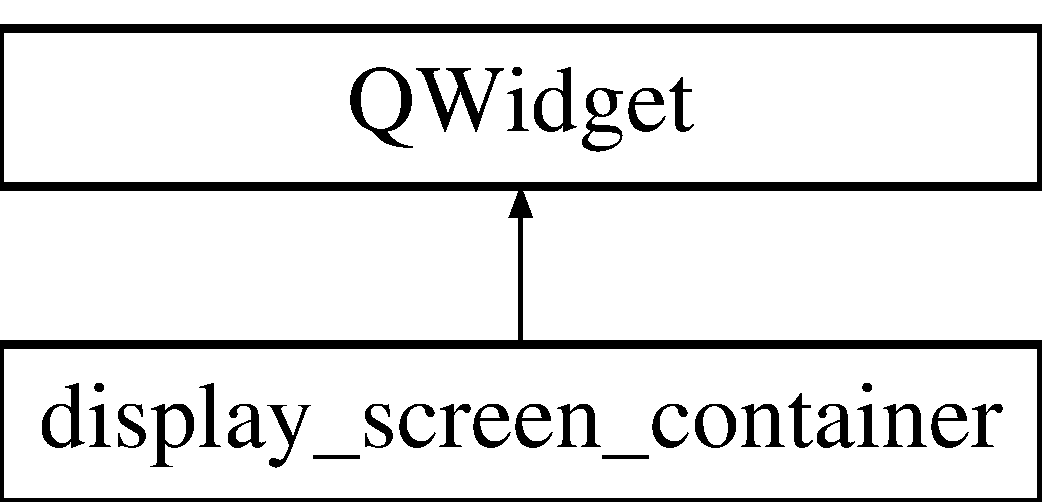
\includegraphics[height=2.000000cm]{classdisplay__screen__container}
\end{center}
\end{figure}
\subsection*{Public Slots}
\begin{DoxyCompactItemize}
\item 
\mbox{\Hypertarget{classdisplay__screen__container_ad136b303dffb379e6f34eebed05e0915}\label{classdisplay__screen__container_ad136b303dffb379e6f34eebed05e0915}} 
void {\bfseries set\+Color\+Map} (const qint16 \&)
\end{DoxyCompactItemize}
\subsection*{Signals}
\begin{DoxyCompactItemize}
\item 
\mbox{\Hypertarget{classdisplay__screen__container_afadf19fd35f800a7ba622fa6023b5e36}\label{classdisplay__screen__container_afadf19fd35f800a7ba622fa6023b5e36}} 
void {\bfseries activate\+Screen\+Container} (const qint32 \&)
\item 
\mbox{\Hypertarget{classdisplay__screen__container_a7266b7910994b761c0ab8b772cdd8248}\label{classdisplay__screen__container_a7266b7910994b761c0ab8b772cdd8248}} 
void {\bfseries plot\+Area\+Updated} ()
\item 
\mbox{\Hypertarget{classdisplay__screen__container_a2145ded890fea1868ffbdc076a25eb64}\label{classdisplay__screen__container_a2145ded890fea1868ffbdc076a25eb64}} 
void {\bfseries scrolled} ()
\end{DoxyCompactItemize}
\subsection*{Public Member Functions}
\begin{DoxyCompactItemize}
\item 
\mbox{\Hypertarget{classdisplay__screen__container_aab2bf99421c31cb1665e9c22db1f647f}\label{classdisplay__screen__container_aab2bf99421c31cb1665e9c22db1f647f}} 
{\bfseries display\+\_\+screen\+\_\+container} (Q\+Widget $\ast$parent=0, \mbox{\hyperlink{classViewer_1_1SimpleVector3D}{Simple\+Vector3D}}$<$ int $>$ $\ast$master\+Cur=0)
\item 
\mbox{\Hypertarget{classdisplay__screen__container_a80401ba88f8bb7948c92885bf63df199}\label{classdisplay__screen__container_a80401ba88f8bb7948c92885bf63df199}} 
void {\bfseries set\+View\+Orientation} (const Orientation \&\+\_\+o)
\item 
\mbox{\Hypertarget{classdisplay__screen__container_a9e7e3ea8326eb4d608bdcbffbc27fe4f}\label{classdisplay__screen__container_a9e7e3ea8326eb4d608bdcbffbc27fe4f}} 
void {\bfseries update\+Plot\+Area} ()
\item 
\mbox{\Hypertarget{classdisplay__screen__container_a8782d999fcd57ef6abd3b9bc0439b17e}\label{classdisplay__screen__container_a8782d999fcd57ef6abd3b9bc0439b17e}} 
std\+::shared\+\_\+ptr$<$ \mbox{\hyperlink{classdisplay__screen}{display\+\_\+screen}} $>$ {\bfseries get\+Active\+Screen} () const
\item 
\mbox{\Hypertarget{classdisplay__screen__container_a76b640770a87c25b9c90ab31d1416bf7}\label{classdisplay__screen__container_a76b640770a87c25b9c90ab31d1416bf7}} 
void {\bfseries actually\+Scroll} (const int \&value)
\item 
\mbox{\Hypertarget{classdisplay__screen__container_a50ff4dd02e4d9d6b2e2485755800e6a2}\label{classdisplay__screen__container_a50ff4dd02e4d9d6b2e2485755800e6a2}} 
qint16 {\bfseries get\+Color\+Map\+Index} () const
\item 
\mbox{\Hypertarget{classdisplay__screen__container_a2a74ef695fda8ea90ea71e11335bb7eb}\label{classdisplay__screen__container_a2a74ef695fda8ea90ea71e11335bb7eb}} 
void {\bfseries set\+Discretised\+Density\+\_\+sptr} (std\+::shared\+\_\+ptr$<$ Discretised\+Density$<$ 3, float $>$ $>$ \+\_\+d)
\item 
\mbox{\Hypertarget{classdisplay__screen__container_adbad3631ce9b6b6bf4c6cb2f611b394b}\label{classdisplay__screen__container_adbad3631ce9b6b6bf4c6cb2f611b394b}} 
const Orientation $\ast$ {\bfseries get\+Orientation} () const
\item 
\mbox{\Hypertarget{classdisplay__screen__container_ade0146a0c568c4c4ed12dec01dabd7ef}\label{classdisplay__screen__container_ade0146a0c568c4c4ed12dec01dabd7ef}} 
void {\bfseries set\+Address\+At\+Parent} (const qint32 \&id)
\item 
\mbox{\Hypertarget{classdisplay__screen__container_a1da8af8c20ea964d082e6e31a8a331f8}\label{classdisplay__screen__container_a1da8af8c20ea964d082e6e31a8a331f8}} 
virtual void {\bfseries mouse\+Press\+Event} (Q\+Mouse\+Event $\ast$event)
\item 
\mbox{\Hypertarget{classdisplay__screen__container_afb58d6b90622e4f2f949cb76237a0c73}\label{classdisplay__screen__container_afb58d6b90622e4f2f949cb76237a0c73}} 
void {\bfseries set\+\_\+active} (bool state)
\item 
\mbox{\Hypertarget{classdisplay__screen__container_a42b1b96f4d570e1e87566855dfec5898}\label{classdisplay__screen__container_a42b1b96f4d570e1e87566855dfec5898}} 
void {\bfseries show\+Cursor} (const bool \&\+\_\+s, const \mbox{\hyperlink{classViewer_1_1SimpleVector2D}{Simple\+Vector2D}}$<$ int $>$ \&\+\_\+cur)
\item 
\mbox{\Hypertarget{classdisplay__screen__container_a335935ef0bd82f657fe47cb14d93bf96}\label{classdisplay__screen__container_a335935ef0bd82f657fe47cb14d93bf96}} 
\mbox{\hyperlink{classViewer_1_1SimpleVector2D}{Viewer\+::\+Simple\+Vector2D}}$<$ int $>$ {\bfseries show\+Cursor} (const bool \&\+\_\+s, const Q\+Point \&\+\_\+cur)
\item 
\mbox{\Hypertarget{classdisplay__screen__container_aac3a1d389e38542d1a1437af139baa30}\label{classdisplay__screen__container_aac3a1d389e38542d1a1437af139baa30}} 
void {\bfseries get\+Cursor\+From\+Point} (const Q\+PointF \&\+\_\+p, \mbox{\hyperlink{classViewer_1_1SimpleVector2D}{Viewer\+::\+Simple\+Vector2D}}$<$ int $>$ \&\+\_\+c)
\item 
\mbox{\Hypertarget{classdisplay__screen__container_ae6ade785282dec1d7096bf922230e363}\label{classdisplay__screen__container_ae6ade785282dec1d7096bf922230e363}} 
int {\bfseries get\+Min\+Pos} () const
\item 
\mbox{\Hypertarget{classdisplay__screen__container_a1ae765f62dce67082596a45dcc4f75bf}\label{classdisplay__screen__container_a1ae765f62dce67082596a45dcc4f75bf}} 
int {\bfseries get\+Max\+Pos} () const
\item 
\mbox{\Hypertarget{classdisplay__screen__container_a4a5a6823fd38e46a780268d0b380012c}\label{classdisplay__screen__container_a4a5a6823fd38e46a780268d0b380012c}} 
void \mbox{\hyperlink{classdisplay__screen__container_a4a5a6823fd38e46a780268d0b380012c}{refresh\+Plot\+Area}} ()
\begin{DoxyCompactList}\small\item\em A light function to trigger the display\+\_\+screen\+::replot\+\_\+me() function. \end{DoxyCompactList}\end{DoxyCompactItemize}
\subsection*{Public Attributes}
\begin{DoxyCompactItemize}
\item 
\mbox{\Hypertarget{classdisplay__screen__container_a44ac856ccf56e16f62714678fa6664a4}\label{classdisplay__screen__container_a44ac856ccf56e16f62714678fa6664a4}} 
Q\+Vector$<$ std\+::shared\+\_\+ptr$<$ \mbox{\hyperlink{classdisplay__screen}{display\+\_\+screen}} $>$ $>$ {\bfseries my\+\_\+screens}
\end{DoxyCompactItemize}


\subsection{Detailed Description}
An interaction interface between screen\+\_\+manager and \mbox{\hyperlink{classdisplay__screen}{display\+\_\+screen}}. It will sort out sizes, Orientation and scrolling between differetn positions 

The documentation for this class was generated from the following files\+:\begin{DoxyCompactItemize}
\item 
src/display\+\_\+buildblock/display\+\_\+screen\+\_\+container.\+h\item 
src/display\+\_\+buildblock/display\+\_\+screen\+\_\+container.\+cpp\end{DoxyCompactItemize}

\hypertarget{classdisplay__screen__curve}{}\section{display\+\_\+screen\+\_\+curve Class Reference}
\label{classdisplay__screen__curve}\index{display\+\_\+screen\+\_\+curve@{display\+\_\+screen\+\_\+curve}}
Inheritance diagram for display\+\_\+screen\+\_\+curve\+:\begin{figure}[H]
\begin{center}
\leavevmode
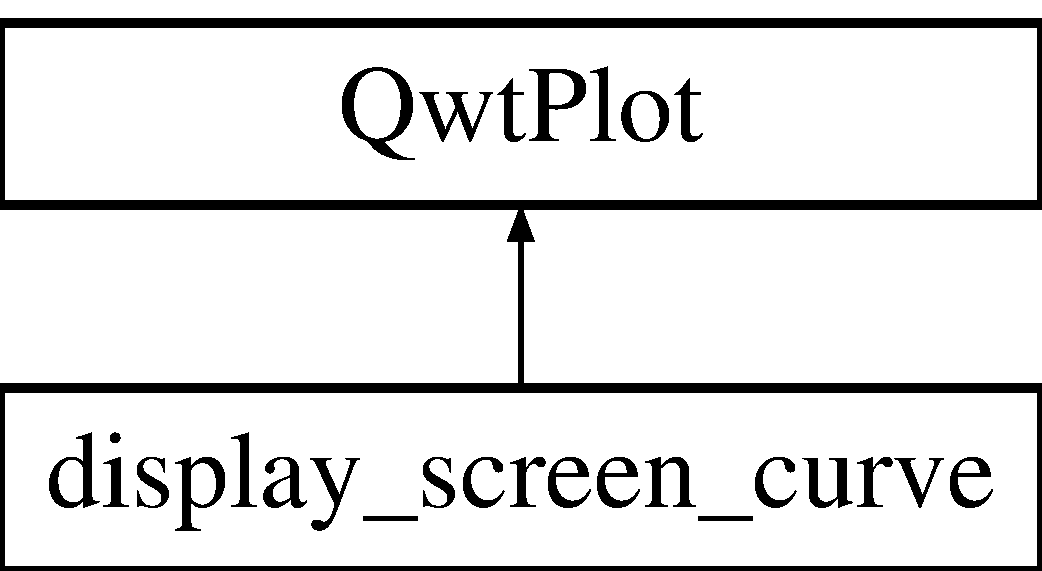
\includegraphics[height=2.000000cm]{classdisplay__screen__curve}
\end{center}
\end{figure}
\subsection*{Public Member Functions}
\begin{DoxyCompactItemize}
\item 
\mbox{\Hypertarget{classdisplay__screen__curve_aabb76c64ffd5643c962e39d539a3ea2e}\label{classdisplay__screen__curve_aabb76c64ffd5643c962e39d539a3ea2e}} 
{\bfseries display\+\_\+screen\+\_\+curve} (Q\+Widget $\ast$parent=0)
\end{DoxyCompactItemize}


The documentation for this class was generated from the following files\+:\begin{DoxyCompactItemize}
\item 
src/display\+\_\+buildblock/display\+\_\+screen\+\_\+curve.\+h\item 
src/display\+\_\+buildblock/display\+\_\+screen\+\_\+curve.\+cpp\end{DoxyCompactItemize}

\hypertarget{classdisplay__screen__raster}{}\section{display\+\_\+screen\+\_\+raster Class Reference}
\label{classdisplay__screen__raster}\index{display\+\_\+screen\+\_\+raster@{display\+\_\+screen\+\_\+raster}}
Inheritance diagram for display\+\_\+screen\+\_\+raster\+:\begin{figure}[H]
\begin{center}
\leavevmode
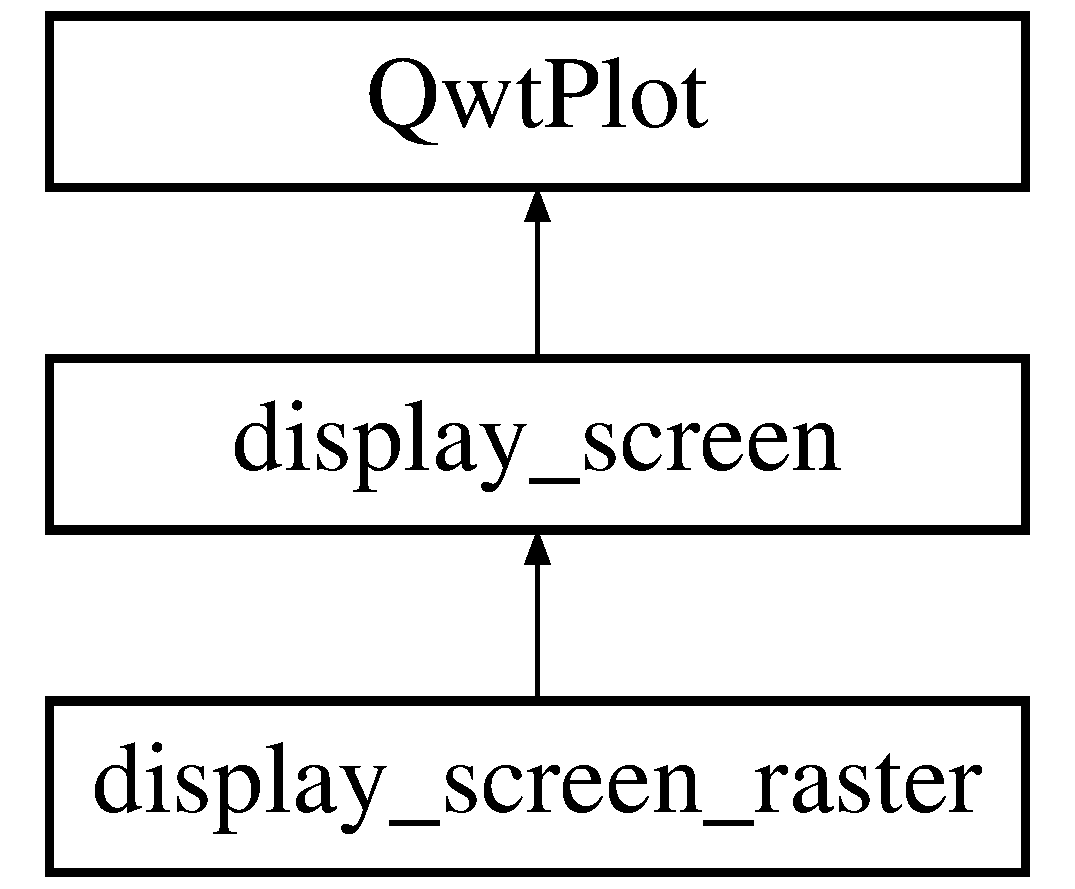
\includegraphics[height=3.000000cm]{classdisplay__screen__raster}
\end{center}
\end{figure}
\subsection*{Public Slots}
\begin{DoxyCompactItemize}
\item 
\mbox{\Hypertarget{classdisplay__screen__raster_afef6f6c99df90e06b993505646f2bb15}\label{classdisplay__screen__raster_afef6f6c99df90e06b993505646f2bb15}} 
void {\bfseries set\+Color\+Map} (const qint16 \&)
\end{DoxyCompactItemize}
\subsection*{Signals}
\begin{DoxyCompactItemize}
\item 
\mbox{\Hypertarget{classdisplay__screen__raster_aec2ac79a9c9269cfb8544ae37fb12e9e}\label{classdisplay__screen__raster_aec2ac79a9c9269cfb8544ae37fb12e9e}} 
void {\bfseries save\+\_\+this\+\_\+array} (int)
\item 
\mbox{\Hypertarget{classdisplay__screen_ac606cfb3c58cd90b354c1b6997737074}\label{classdisplay__screen_ac606cfb3c58cd90b354c1b6997737074}} 
void {\bfseries activate\+Screen} (const qint32 \&)
\end{DoxyCompactItemize}
\subsection*{Public Member Functions}
\begin{DoxyCompactItemize}
\item 
\mbox{\Hypertarget{classdisplay__screen__raster_a045c1bd61ae9dedad1600568f8db18c1}\label{classdisplay__screen__raster_a045c1bd61ae9dedad1600568f8db18c1}} 
{\bfseries display\+\_\+screen\+\_\+raster} (Q\+Widget $\ast$parent=0)
\item 
\mbox{\Hypertarget{classdisplay__screen__raster_ab148d22834c5bb1c69087cd64388b1fc}\label{classdisplay__screen__raster_ab148d22834c5bb1c69087cd64388b1fc}} 
void {\bfseries replot\+\_\+me} ()
\item 
\mbox{\Hypertarget{classdisplay__screen__raster_ac800eb58bc8e9c2cbb8b9481fc3b38cf}\label{classdisplay__screen__raster_ac800eb58bc8e9c2cbb8b9481fc3b38cf}} 
void {\bfseries set\+\_\+sizes} (const int \&\+\_\+h, const int \&\+\_\+v, const int \&\+\_\+min\+\_\+index\+\_\+h, const int \&\+\_\+min\+\_\+index\+\_\+v, const int \&\+\_\+max\+\_\+index\+\_\+h, const int \&\+\_\+max\+\_\+index\+\_\+v, const float \&\+\_\+h\+\_\+spacing, const float \&\+\_\+v\+\_\+spacing, const float \&min\+\_\+x, const float \&max\+\_\+x, const float \&min\+\_\+y, const float \&max\+\_\+y)
\item 
\mbox{\Hypertarget{classdisplay__screen__raster_a4a5d5ee25ba19ff6b7773674325d13ff}\label{classdisplay__screen__raster_a4a5d5ee25ba19ff6b7773674325d13ff}} 
void {\bfseries draw\+\_\+curve} (const Q\+Vector$<$ Q\+PointF $>$ \&)
\item 
\mbox{\Hypertarget{classdisplay__screen__raster_ac0bebdf7c91a9a14295960cc837b4989}\label{classdisplay__screen__raster_ac0bebdf7c91a9a14295960cc837b4989}} 
virtual void {\bfseries set\+O\+CD} (const Q\+String \&\+\_\+l, const Q\+String \&\+\_\+r, const Q\+String \&\+\_\+t, const Q\+String \&\+\_\+b)
\item 
\mbox{\Hypertarget{classdisplay__screen__raster_a3a06d6a7a37ae3ceac4a251e5cea5f2a}\label{classdisplay__screen__raster_a3a06d6a7a37ae3ceac4a251e5cea5f2a}} 
virtual void {\bfseries set\+My\+Title} (const qint32 \&\+\_\+label)
\item 
\mbox{\Hypertarget{classdisplay__screen__raster_aa715e923b2f425f878011f34f3efa148}\label{classdisplay__screen__raster_aa715e923b2f425f878011f34f3efa148}} 
void {\bfseries set\+\_\+max\+\_\+value} (const double \&new\+\_\+max)
\item 
\mbox{\Hypertarget{classdisplay__screen__raster_a8a4da270a9fc4269dffc86c3a80463d0}\label{classdisplay__screen__raster_a8a4da270a9fc4269dffc86c3a80463d0}} 
void {\bfseries set\+\_\+min\+\_\+value} (const double \&new\+\_\+min)
\item 
\mbox{\Hypertarget{classdisplay__screen__raster_afd08c36c3a75cae7b3ffab7acee90b90}\label{classdisplay__screen__raster_afd08c36c3a75cae7b3ffab7acee90b90}} 
void {\bfseries set\+\_\+min\+\_\+max\+\_\+values} (const double \&new\+\_\+min, const double \&new\+\_\+max)
\item 
\mbox{\Hypertarget{classdisplay__screen__raster_ab13b2d6bbfce1b21386136eef65bbbef}\label{classdisplay__screen__raster_ab13b2d6bbfce1b21386136eef65bbbef}} 
Q\+Vector$<$ double $>$\+::iterator {\bfseries get\+\_\+data\+\_\+begin} ()
\item 
\mbox{\Hypertarget{classdisplay__screen__raster_a23ddb56ac7a520bfea79420043ef1bbc}\label{classdisplay__screen__raster_a23ddb56ac7a520bfea79420043ef1bbc}} 
Q\+Vector$<$ double $>$\+::iterator {\bfseries get\+\_\+data\+\_\+end} ()
\item 
\mbox{\Hypertarget{classdisplay__screen__raster_a0e242ba6b3b79f336d548b13ab25d74e}\label{classdisplay__screen__raster_a0e242ba6b3b79f336d548b13ab25d74e}} 
Q\+Vector$<$ double $>$\+::Const\+Iterator {\bfseries get\+\_\+data\+\_\+const\+\_\+begin} () const
\item 
\mbox{\Hypertarget{classdisplay__screen__raster_a53b12f7bae3d50b197e16574efbeeccb}\label{classdisplay__screen__raster_a53b12f7bae3d50b197e16574efbeeccb}} 
Q\+Vector$<$ double $>$\+::Const\+Iterator {\bfseries get\+\_\+data\+\_\+const\+\_\+end} () const
\item 
\mbox{\Hypertarget{classdisplay__screen__raster_a173e087eea352bdb14c01eb5d98a6f50}\label{classdisplay__screen__raster_a173e087eea352bdb14c01eb5d98a6f50}} 
const double {\bfseries get\+\_\+max\+\_\+value\+\_\+ptr} () const
\item 
\mbox{\Hypertarget{classdisplay__screen__raster_a08709a1fc188c287f1440f85b48ca976}\label{classdisplay__screen__raster_a08709a1fc188c287f1440f85b48ca976}} 
const double {\bfseries get\+\_\+min\+\_\+value\+\_\+ptr} () const
\item 
void \mbox{\hyperlink{classdisplay__screen__raster_aacbbdf19c624ecb6f09c32c27b6f4132}{set\+Interval}} (const double \&\+\_\+min, const double \&\+\_\+max)
\item 
\mbox{\Hypertarget{classdisplay__screen__raster_aabe35c0294f6bde7f49ba78501fe6f62}\label{classdisplay__screen__raster_aabe35c0294f6bde7f49ba78501fe6f62}} 
void {\bfseries key\+Press\+Event} (Q\+Key\+Event $\ast$key\+Event) override
\item 
\mbox{\Hypertarget{classdisplay__screen__raster_adf6cfbba94df093fcebc987dc6ca582d}\label{classdisplay__screen__raster_adf6cfbba94df093fcebc987dc6ca582d}} 
void {\bfseries draw\+Cursor} (const bool \&\+\_\+s, const \mbox{\hyperlink{classViewer_1_1SimpleVector2D}{Viewer\+::\+Simple\+Vector2D}}$<$ int $>$ \&ps)
\item 
\mbox{\Hypertarget{classdisplay__screen__raster_a8f54873f88a76ab9155def0e6e8837f4}\label{classdisplay__screen__raster_a8f54873f88a76ab9155def0e6e8837f4}} 
\mbox{\hyperlink{classViewer_1_1SimpleVector2D}{Viewer\+::\+Simple\+Vector2D}}$<$ int $>$ {\bfseries draw\+Cursor} (const bool \&\+\_\+s, const Q\+PointF \&ps)
\item 
\mbox{\Hypertarget{classdisplay__screen__raster_a7a1e51868bb80d1322a15f9024bd8360}\label{classdisplay__screen__raster_a7a1e51868bb80d1322a15f9024bd8360}} 
void {\bfseries xy\+From\+Cell} (const \mbox{\hyperlink{classViewer_1_1SimpleVector2D}{Viewer\+::\+Simple\+Vector2D}}$<$ int $>$ \&, Q\+PointF \&)
\item 
\mbox{\Hypertarget{classdisplay__screen__raster_a9c07112a8c204841669c597486091d33}\label{classdisplay__screen__raster_a9c07112a8c204841669c597486091d33}} 
void {\bfseries cell\+From\+XY} (const Q\+PointF \&\+\_\+p, \mbox{\hyperlink{classViewer_1_1SimpleVector2D}{Viewer\+::\+Simple\+Vector2D}}$<$ int $>$ \&\+\_\+v)
\item 
virtual void \mbox{\hyperlink{classdisplay__screen__raster_a7cfddde7af1d6bb730a43b5cd13af34f}{write\+Values\+In\+Data}} (const stir\+::\+Proj\+Matrix\+Elems\+For\+One\+Bin \&, const float \&)
\item 
\mbox{\Hypertarget{classdisplay__screen__raster_a494cf5aca93f26d87e7d4452c17852b8}\label{classdisplay__screen__raster_a494cf5aca93f26d87e7d4452c17852b8}} 
virtual stir\+::\+Cartesian\+Coordinate3D$<$ float $>$ \mbox{\hyperlink{classdisplay__screen__raster_a494cf5aca93f26d87e7d4452c17852b8}{get\+Grid\+Spacing}} ()
\begin{DoxyCompactList}\small\item\em Return the Pixel hint (or grid spacing of the data) \end{DoxyCompactList}\item 
void \mbox{\hyperlink{classdisplay__screen__raster_a0469e5189411a5b83d6386510832d46d}{clear\+Cursors}} ()
\item 
\mbox{\Hypertarget{classdisplay__screen_a27d55d66129e2f3b99314c73d5457eaf}\label{classdisplay__screen_a27d55d66129e2f3b99314c73d5457eaf}} 
int {\bfseries get\+\_\+data\+\_\+size} ()
\item 
\mbox{\Hypertarget{classdisplay__screen_a85b97edfde46cbe8136877c35bb6876d}\label{classdisplay__screen_a85b97edfde46cbe8136877c35bb6876d}} 
void \mbox{\hyperlink{classdisplay__screen_a85b97edfde46cbe8136877c35bb6876d}{clear\+Curves}} ()
\begin{DoxyCompactList}\small\item\em Remove every curve is on the screen. \end{DoxyCompactList}\item 
\mbox{\Hypertarget{classdisplay__screen_ac2ef804e167c1ba941dcf91134bbe769}\label{classdisplay__screen_ac2ef804e167c1ba941dcf91134bbe769}} 
void {\bfseries set\+\_\+active} (bool state)
\item 
\mbox{\Hypertarget{classdisplay__screen_ac64b0a65402d794e135c6c6e189d02a6}\label{classdisplay__screen_ac64b0a65402d794e135c6c6e189d02a6}} 
virtual void {\bfseries mouse\+Press\+Event} (Q\+Mouse\+Event $\ast$event)
\item 
\mbox{\Hypertarget{classdisplay__screen_ab54ec0811e324d192a75b3e538c66513}\label{classdisplay__screen_ab54ec0811e324d192a75b3e538c66513}} 
void {\bfseries set\+Address\+At\+Parent} (const qint32 \&id)
\item 
\mbox{\Hypertarget{classdisplay__screen_a1a0a574c59e0c4cfd8ad8de4bb8e105d}\label{classdisplay__screen_a1a0a574c59e0c4cfd8ad8de4bb8e105d}} 
const double $\ast$ {\bfseries get\+\_\+max\+\_\+vis\+\_\+value\+\_\+ptr} () const
\item 
\mbox{\Hypertarget{classdisplay__screen_a8e8a2009db3859562e3d52e44731dd03}\label{classdisplay__screen_a8e8a2009db3859562e3d52e44731dd03}} 
const double $\ast$ {\bfseries get\+\_\+min\+\_\+vis\+\_\+value\+\_\+ptr} () const
\item 
\mbox{\Hypertarget{classdisplay__screen_a17b159563b62a3c8bfd7245453ba421a}\label{classdisplay__screen_a17b159563b62a3c8bfd7245453ba421a}} 
void {\bfseries apply\+Function} (\mbox{\hyperlink{classWorker}{Worker}} $\ast$\+\_\+w)
\item 
\mbox{\Hypertarget{classdisplay__screen_a2df277a3abd63d90ec1ead11d0eb3818}\label{classdisplay__screen_a2df277a3abd63d90ec1ead11d0eb3818}} 
void {\bfseries remove\+Function} ()
\end{DoxyCompactItemize}
\subsection*{Protected Slots}
\begin{DoxyCompactItemize}
\item 
\mbox{\Hypertarget{classdisplay__screen__raster_ada409c22c06e97a72216609aa7ff34b9}\label{classdisplay__screen__raster_ada409c22c06e97a72216609aa7ff34b9}} 
virtual void {\bfseries pop\+Up\+Menu} (const Q\+Point \&pos) override
\end{DoxyCompactItemize}
\subsection*{Protected Member Functions}
\begin{DoxyCompactItemize}
\item 
\mbox{\Hypertarget{classdisplay__screen_a5f27a1aa1d1ef02823cdf23a686e5593}\label{classdisplay__screen_a5f27a1aa1d1ef02823cdf23a686e5593}} 
void \mbox{\hyperlink{classdisplay__screen_a5f27a1aa1d1ef02823cdf23a686e5593}{draw\+Selection\+Frame}} (bool state)
\begin{DoxyCompactList}\small\item\em Draw a frame around the display to indicate that this is the active. \end{DoxyCompactList}\end{DoxyCompactItemize}
\subsection*{Protected Attributes}
\begin{DoxyCompactItemize}
\item 
\mbox{\Hypertarget{classdisplay__screen_a52bf41a53070ae85bdf46ee75dd84f0d}\label{classdisplay__screen_a52bf41a53070ae85bdf46ee75dd84f0d}} 
Q\+Vector$<$ double $>$ \mbox{\hyperlink{classdisplay__screen_a52bf41a53070ae85bdf46ee75dd84f0d}{my\+\_\+data}}
\begin{DoxyCompactList}\small\item\em The data which are displayed on screen. \end{DoxyCompactList}\item 
\mbox{\Hypertarget{classdisplay__screen_a404e8f942e20b528e8017f693eea5ea5}\label{classdisplay__screen_a404e8f942e20b528e8017f693eea5ea5}} 
qint32 {\bfseries my\+Address}
\item 
\mbox{\Hypertarget{classdisplay__screen_aa5d0a895e06f256254d60c9a6761353a}\label{classdisplay__screen_aa5d0a895e06f256254d60c9a6761353a}} 
qint32 \mbox{\hyperlink{classdisplay__screen_aa5d0a895e06f256254d60c9a6761353a}{my\+\_\+label}}
\begin{DoxyCompactList}\small\item\em The number displayed at the bottom right corner. In sync with the scroll bar. \end{DoxyCompactList}\item 
\mbox{\Hypertarget{classdisplay__screen_aa36da095bb12f0f4c9a5063fc9477bf8}\label{classdisplay__screen_aa36da095bb12f0f4c9a5063fc9477bf8}} 
int {\bfseries size}
\item 
\mbox{\Hypertarget{classdisplay__screen_aefb44f5edee20d8ec3f1e6f1cb790db4}\label{classdisplay__screen_aefb44f5edee20d8ec3f1e6f1cb790db4}} 
bool {\bfseries cursor\+Status}
\item 
\mbox{\Hypertarget{classdisplay__screen_a456d4c817042e690b69f978fdbf16320}\label{classdisplay__screen_a456d4c817042e690b69f978fdbf16320}} 
Qwt\+Plot\+Text\+Label $\ast$ {\bfseries title\+Item}
\item 
\mbox{\Hypertarget{classdisplay__screen_ae6764a9d2d77f51e93cdc34ab277d48a}\label{classdisplay__screen_ae6764a9d2d77f51e93cdc34ab277d48a}} 
Qwt\+Plot\+Text\+Label $\ast$ {\bfseries l\+O\+C\+D\+Item}
\item 
\mbox{\Hypertarget{classdisplay__screen_a69d982deaa57cd6d447b7408093568a6}\label{classdisplay__screen_a69d982deaa57cd6d447b7408093568a6}} 
Qwt\+Plot\+Text\+Label $\ast$ {\bfseries r\+O\+C\+D\+Item}
\item 
\mbox{\Hypertarget{classdisplay__screen_a570edfafbba0d70fce7d9967958310aa}\label{classdisplay__screen_a570edfafbba0d70fce7d9967958310aa}} 
Qwt\+Plot\+Text\+Label $\ast$ {\bfseries b\+O\+C\+D\+Item}
\item 
\mbox{\Hypertarget{classdisplay__screen_a8faeeea1ba78a88dae699c43fa0ae087}\label{classdisplay__screen_a8faeeea1ba78a88dae699c43fa0ae087}} 
Qwt\+Plot\+Text\+Label $\ast$ {\bfseries t\+O\+C\+D\+Item}
\item 
\mbox{\Hypertarget{classdisplay__screen_a7babe15db1f589f15bb94c6f54a7c9fb}\label{classdisplay__screen_a7babe15db1f589f15bb94c6f54a7c9fb}} 
Q\+Font \mbox{\hyperlink{classdisplay__screen_a7babe15db1f589f15bb94c6f54a7c9fb}{font}}
\begin{DoxyCompactList}\small\item\em The font used for the O\+CD text. \end{DoxyCompactList}\item 
\mbox{\Hypertarget{classdisplay__screen_ad22570d6a6e8ed9b46f9040406ad812c}\label{classdisplay__screen_ad22570d6a6e8ed9b46f9040406ad812c}} 
Qwt\+Text \mbox{\hyperlink{classdisplay__screen_ad22570d6a6e8ed9b46f9040406ad812c}{title}}
\begin{DoxyCompactList}\small\item\em Text for the O\+CD texts. \end{DoxyCompactList}\item 
\mbox{\Hypertarget{classdisplay__screen_a8cd4a91142663ac54195431d5cd60e9d}\label{classdisplay__screen_a8cd4a91142663ac54195431d5cd60e9d}} 
Qwt\+Text {\bfseries l\+O\+CD}
\item 
\mbox{\Hypertarget{classdisplay__screen_aa622bfa993c2bec08e31f78b91fd4d2b}\label{classdisplay__screen_aa622bfa993c2bec08e31f78b91fd4d2b}} 
Qwt\+Text {\bfseries r\+O\+CD}
\item 
\mbox{\Hypertarget{classdisplay__screen_a050d88f65c01662ab2b637bfa90c7abd}\label{classdisplay__screen_a050d88f65c01662ab2b637bfa90c7abd}} 
Qwt\+Text {\bfseries b\+O\+CD}
\item 
\mbox{\Hypertarget{classdisplay__screen_a099a94fac1e3c0bab6884c8953a43031}\label{classdisplay__screen_a099a94fac1e3c0bab6884c8953a43031}} 
Qwt\+Text {\bfseries t\+O\+CD}
\item 
\mbox{\Hypertarget{classdisplay__screen_a7ffb415729f7d3d10505ac04f829582c}\label{classdisplay__screen_a7ffb415729f7d3d10505ac04f829582c}} 
double \mbox{\hyperlink{classdisplay__screen_a7ffb415729f7d3d10505ac04f829582c}{max\+\_\+value}}
\begin{DoxyCompactList}\small\item\em Max value of the display data. \end{DoxyCompactList}\item 
\mbox{\Hypertarget{classdisplay__screen_a3091e35b28219274fe9ffd8e8dc68c40}\label{classdisplay__screen_a3091e35b28219274fe9ffd8e8dc68c40}} 
double \mbox{\hyperlink{classdisplay__screen_a3091e35b28219274fe9ffd8e8dc68c40}{min\+\_\+value}}
\begin{DoxyCompactList}\small\item\em Min value of the display data. \end{DoxyCompactList}\item 
\mbox{\Hypertarget{classdisplay__screen_a0a040ebfadeba044ee2d887c43b37425}\label{classdisplay__screen_a0a040ebfadeba044ee2d887c43b37425}} 
double \mbox{\hyperlink{classdisplay__screen_a0a040ebfadeba044ee2d887c43b37425}{vis\+\_\+min}}
\begin{DoxyCompactList}\small\item\em Apparent min value -\/ W\&L operations set this value. \end{DoxyCompactList}\item 
\mbox{\Hypertarget{classdisplay__screen_a100a772813944bb4a41feab579ae11d8}\label{classdisplay__screen_a100a772813944bb4a41feab579ae11d8}} 
double \mbox{\hyperlink{classdisplay__screen_a100a772813944bb4a41feab579ae11d8}{vis\+\_\+max}}
\begin{DoxyCompactList}\small\item\em Apparent max value -\/ W\&L operations set this value. \end{DoxyCompactList}\item 
\mbox{\hyperlink{classWorker}{Worker}} $\ast$ \mbox{\hyperlink{classdisplay__screen_a54ed0638f240e4a044d9d4376233ec71}{filter}}
\end{DoxyCompactItemize}


\subsection{Member Function Documentation}
\mbox{\Hypertarget{classdisplay__screen__raster_a0469e5189411a5b83d6386510832d46d}\label{classdisplay__screen__raster_a0469e5189411a5b83d6386510832d46d}} 
\index{display\+\_\+screen\+\_\+raster@{display\+\_\+screen\+\_\+raster}!clear\+Cursors@{clear\+Cursors}}
\index{clear\+Cursors@{clear\+Cursors}!display\+\_\+screen\+\_\+raster@{display\+\_\+screen\+\_\+raster}}
\subsubsection{\texorpdfstring{clear\+Cursors()}{clearCursors()}}
{\footnotesize\ttfamily void display\+\_\+screen\+\_\+raster\+::clear\+Cursors (\begin{DoxyParamCaption}{ }\end{DoxyParamCaption})\hspace{0.3cm}{\ttfamily [virtual]}}

Remove the cross section which indicates the current position of the cursor. 

Implements \mbox{\hyperlink{classdisplay__screen_aedda58c57969f054fb9bedd1ed01b62c}{display\+\_\+screen}}.

\mbox{\Hypertarget{classdisplay__screen__raster_aacbbdf19c624ecb6f09c32c27b6f4132}\label{classdisplay__screen__raster_aacbbdf19c624ecb6f09c32c27b6f4132}} 
\index{display\+\_\+screen\+\_\+raster@{display\+\_\+screen\+\_\+raster}!set\+Interval@{set\+Interval}}
\index{set\+Interval@{set\+Interval}!display\+\_\+screen\+\_\+raster@{display\+\_\+screen\+\_\+raster}}
\subsubsection{\texorpdfstring{set\+Interval()}{setInterval()}}
{\footnotesize\ttfamily void display\+\_\+screen\+\_\+raster\+::set\+Interval (\begin{DoxyParamCaption}\item[{const double \&}]{\+\_\+min,  }\item[{const double \&}]{\+\_\+max }\end{DoxyParamCaption})\hspace{0.3cm}{\ttfamily [virtual]}}

Sets the vis\+\_\+min and vis\+\_\+max values. Essentially this affects the W\&L operations on the display. 

Implements \mbox{\hyperlink{classdisplay__screen}{display\+\_\+screen}}.

\mbox{\Hypertarget{classdisplay__screen__raster_a7cfddde7af1d6bb730a43b5cd13af34f}\label{classdisplay__screen__raster_a7cfddde7af1d6bb730a43b5cd13af34f}} 
\index{display\+\_\+screen\+\_\+raster@{display\+\_\+screen\+\_\+raster}!write\+Values\+In\+Data@{write\+Values\+In\+Data}}
\index{write\+Values\+In\+Data@{write\+Values\+In\+Data}!display\+\_\+screen\+\_\+raster@{display\+\_\+screen\+\_\+raster}}
\subsubsection{\texorpdfstring{write\+Values\+In\+Data()}{writeValuesInData()}}
{\footnotesize\ttfamily void display\+\_\+screen\+\_\+raster\+::write\+Values\+In\+Data (\begin{DoxyParamCaption}\item[{const stir\+::\+Proj\+Matrix\+Elems\+For\+One\+Bin \&}]{,  }\item[{const float \&}]{ }\end{DoxyParamCaption})\hspace{0.3cm}{\ttfamily [virtual]}}

Change the value of particular pixels in the raster. This function initially is make to test the location of the profiles In the future might become a fully operational fuction. 

Implements \mbox{\hyperlink{classdisplay__screen_a2788f315d8f91b4c8a2b870698ce6623}{display\+\_\+screen}}.



\subsection{Member Data Documentation}
\mbox{\Hypertarget{classdisplay__screen_a54ed0638f240e4a044d9d4376233ec71}\label{classdisplay__screen_a54ed0638f240e4a044d9d4376233ec71}} 
\index{display\+\_\+screen\+\_\+raster@{display\+\_\+screen\+\_\+raster}!filter@{filter}}
\index{filter@{filter}!display\+\_\+screen\+\_\+raster@{display\+\_\+screen\+\_\+raster}}
\subsubsection{\texorpdfstring{filter}{filter}}
{\footnotesize\ttfamily \mbox{\hyperlink{classWorker}{Worker}}$\ast$ display\+\_\+screen\+::filter\hspace{0.3cm}{\ttfamily [protected]}, {\ttfamily [inherited]}}

This is a somewhat agly workaround. When a function has to be applied on the my\+\_\+data Q\+Vector in order to preview the effect of a filter. 

The documentation for this class was generated from the following files\+:\begin{DoxyCompactItemize}
\item 
src/display\+\_\+buildblock/display\+\_\+screen\+\_\+raster.\+h\item 
src/display\+\_\+buildblock/display\+\_\+screen.\+inl\item 
src/display\+\_\+buildblock/display\+\_\+screen\+\_\+raster.\+cpp\end{DoxyCompactItemize}

\hypertarget{classEclipseTool}{}\section{Eclipse\+Tool Class Reference}
\label{classEclipseTool}\index{Eclipse\+Tool@{Eclipse\+Tool}}
Inheritance diagram for Eclipse\+Tool\+:\begin{figure}[H]
\begin{center}
\leavevmode
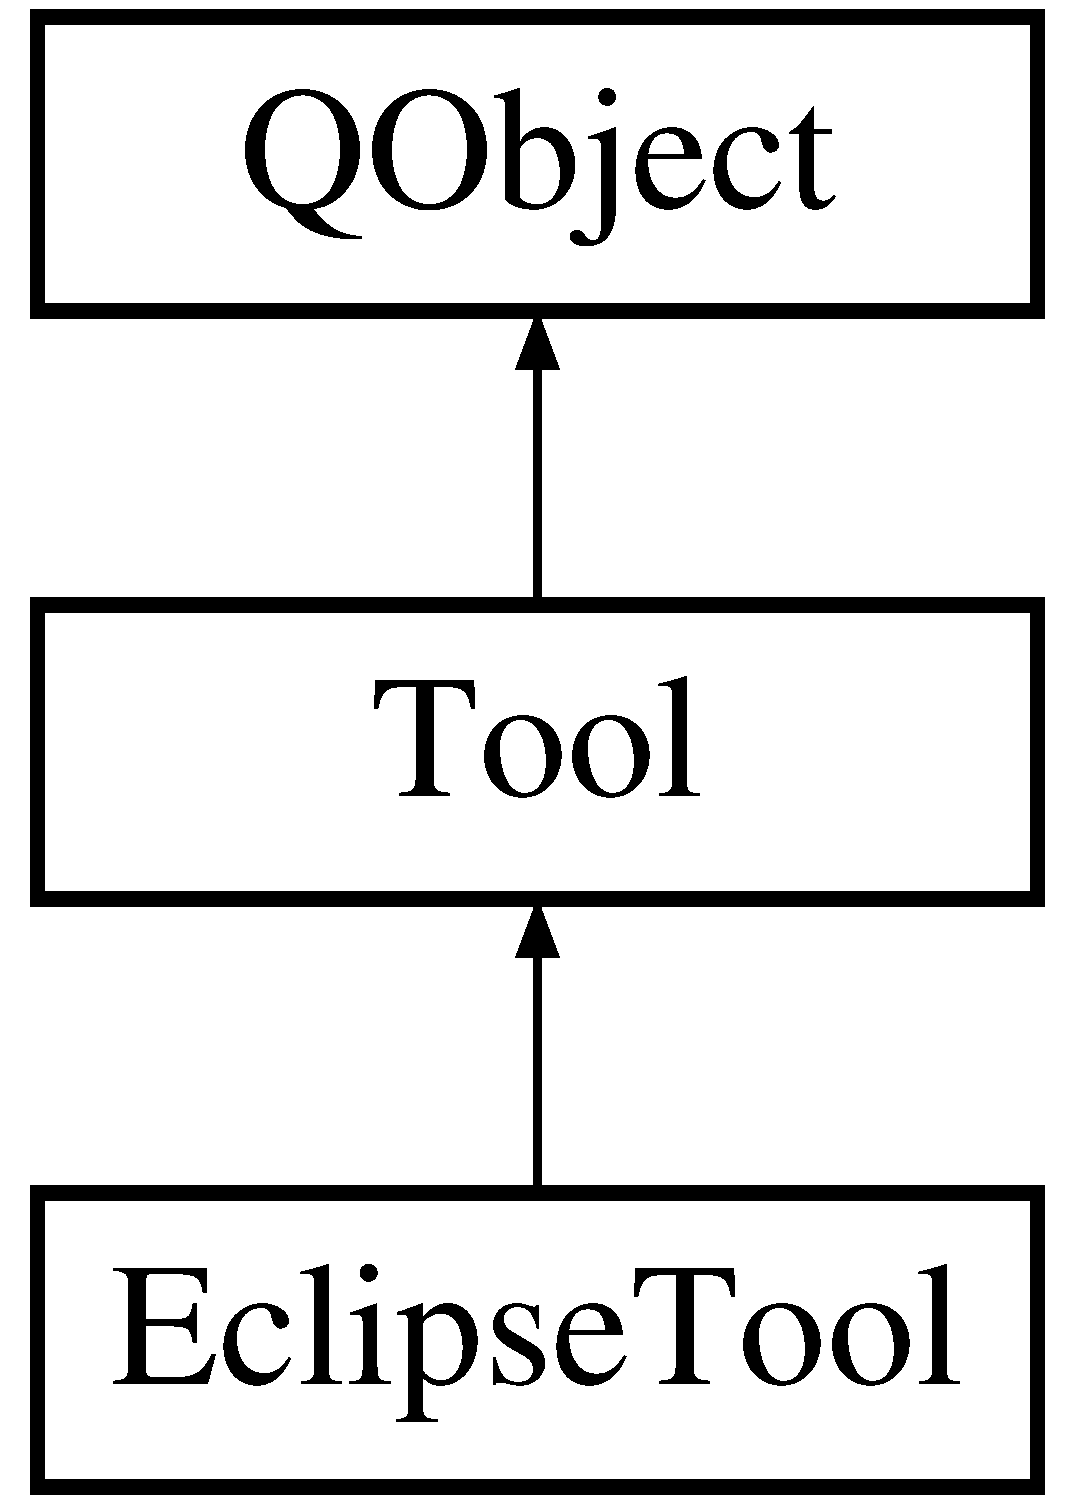
\includegraphics[height=3.000000cm]{classEclipseTool}
\end{center}
\end{figure}
\subsection*{Signals}
\begin{DoxyCompactItemize}
\item 
\mbox{\Hypertarget{classTool_a68dea3e4c911f3174176084d350865cc}\label{classTool_a68dea3e4c911f3174176084d350865cc}} 
void {\bfseries this\+\_\+selection} (const Q\+Vector$<$ Q\+PointF $>$ \&, Qwt\+Plot $\ast$)
\end{DoxyCompactItemize}
\subsection*{Public Member Functions}
\begin{DoxyCompactItemize}
\item 
\mbox{\Hypertarget{classEclipseTool_abc2b8f954c0c83f31b37b759f07f7f40}\label{classEclipseTool_abc2b8f954c0c83f31b37b759f07f7f40}} 
{\bfseries Eclipse\+Tool} (Q\+Object $\ast$parent=nullptr)
\item 
\mbox{\Hypertarget{classTool_a020bd5757a03ea7321848a3874f3a8cb}\label{classTool_a020bd5757a03ea7321848a3874f3a8cb}} 
virtual bool {\bfseries event\+Filter} (Q\+Object $\ast$, Q\+Event $\ast$)
\item 
\mbox{\Hypertarget{classTool_aa30c64915020a71d0ea8650e8e966336}\label{classTool_aa30c64915020a71d0ea8650e8e966336}} 
virtual Q\+String {\bfseries get\+\_\+name} () const
\item 
\mbox{\Hypertarget{classTool_a5cb18e4c28ab3d8d39535db5d2213c81}\label{classTool_a5cb18e4c28ab3d8d39535db5d2213c81}} 
virtual void {\bfseries finished\+Selecting} ()=0
\item 
\mbox{\Hypertarget{classTool_a507adfcdafc818d9628b952001b93f3c}\label{classTool_a507adfcdafc818d9628b952001b93f3c}} 
void {\bfseries get\+\_\+data} (Q\+Vector$<$ Q\+PointF $>$ \&, Qwt\+Plot $\ast$)
\item 
virtual void \mbox{\hyperlink{classTool_a7d9e7d03f4a34d71850cbbfc16ca8532}{clear\+Before\+Un\+Set}} ()=0
\end{DoxyCompactItemize}
\subsection*{Protected Member Functions}
\begin{DoxyCompactItemize}
\item 
\mbox{\Hypertarget{classTool_a11f1da4092d196a7b91d3d60276586eb}\label{classTool_a11f1da4092d196a7b91d3d60276586eb}} 
virtual void \mbox{\hyperlink{classTool_a11f1da4092d196a7b91d3d60276586eb}{clear\+Selection}} ()
\begin{DoxyCompactList}\small\item\em Remove all curves from the c\+\_\+paint\+Device. \end{DoxyCompactList}\item 
bool \mbox{\hyperlink{classTool_a81244366dc1b9f55465ed6f37b81033c}{check\+Point\+In\+Range}} (const Q\+PointF \&\+\_\+local)
\item 
\mbox{\Hypertarget{classTool_a453549f925313d28b19fc9a81aabfe01}\label{classTool_a453549f925313d28b19fc9a81aabfe01}} 
virtual void \mbox{\hyperlink{classTool_a453549f925313d28b19fc9a81aabfe01}{select}} (const Q\+PointF \&)=0
\begin{DoxyCompactList}\small\item\em On mouse press action. \end{DoxyCompactList}\item 
\mbox{\Hypertarget{classTool_a734b60b6ecf4b9fa2e56186349a5a3cf}\label{classTool_a734b60b6ecf4b9fa2e56186349a5a3cf}} 
virtual void \mbox{\hyperlink{classTool_a734b60b6ecf4b9fa2e56186349a5a3cf}{move}} (const Q\+PointF \&)=0
\begin{DoxyCompactList}\small\item\em On mouse press and drag action. \end{DoxyCompactList}\end{DoxyCompactItemize}
\subsection*{Protected Attributes}
\begin{DoxyCompactItemize}
\item 
\mbox{\Hypertarget{classTool_af0935d8e8edd73d8ec85424b5b15196b}\label{classTool_af0935d8e8edd73d8ec85424b5b15196b}} 
Q\+String {\bfseries name}
\item 
\mbox{\Hypertarget{classTool_a1e301a03c5806c900786760d80049380}\label{classTool_a1e301a03c5806c900786760d80049380}} 
Qwt\+Plot\+Canvas $\ast$ {\bfseries c\+\_\+paint\+Device}
\item 
\mbox{\Hypertarget{classTool_af1d11cc5374ba7eb7c1d41cfb5d4e981}\label{classTool_af1d11cc5374ba7eb7c1d41cfb5d4e981}} 
Qwt\+Plot\+Spectrogram $\ast$ {\bfseries d\+\_\+spectrogram}
\item 
Q\+Vector$<$ Q\+PointF $>$ \mbox{\hyperlink{classTool_a68be77a2e364a7b13d7206388ba5843e}{\+\_\+points}}
\end{DoxyCompactItemize}


\subsection{Member Function Documentation}
\mbox{\Hypertarget{classTool_a81244366dc1b9f55465ed6f37b81033c}\label{classTool_a81244366dc1b9f55465ed6f37b81033c}} 
\index{Eclipse\+Tool@{Eclipse\+Tool}!check\+Point\+In\+Range@{check\+Point\+In\+Range}}
\index{check\+Point\+In\+Range@{check\+Point\+In\+Range}!Eclipse\+Tool@{Eclipse\+Tool}}
\subsubsection{\texorpdfstring{check\+Point\+In\+Range()}{checkPointInRange()}}
{\footnotesize\ttfamily bool Tool\+::check\+Point\+In\+Range (\begin{DoxyParamCaption}\item[{const Q\+PointF \&}]{\+\_\+local }\end{DoxyParamCaption})\hspace{0.3cm}{\ttfamily [protected]}, {\ttfamily [inherited]}}

This is a preliminiry check to see if the point is within the axis range. It has been proven somewhat week condition, as in many cases it fails to provide realible results. \mbox{\Hypertarget{classTool_a7d9e7d03f4a34d71850cbbfc16ca8532}\label{classTool_a7d9e7d03f4a34d71850cbbfc16ca8532}} 
\index{Eclipse\+Tool@{Eclipse\+Tool}!clear\+Before\+Un\+Set@{clear\+Before\+Un\+Set}}
\index{clear\+Before\+Un\+Set@{clear\+Before\+Un\+Set}!Eclipse\+Tool@{Eclipse\+Tool}}
\subsubsection{\texorpdfstring{clear\+Before\+Un\+Set()}{clearBeforeUnSet()}}
{\footnotesize\ttfamily virtual void Tool\+::clear\+Before\+Un\+Set (\begin{DoxyParamCaption}{ }\end{DoxyParamCaption})\hspace{0.3cm}{\ttfamily [pure virtual]}, {\ttfamily [inherited]}}

Cal this function to clean before unsetting a tool. It will try to tight up the screen. 

Implemented in \mbox{\hyperlink{classPointerTool_a04c325128dc9ee27272eace9e70d15aa}{Pointer\+Tool}}, \mbox{\hyperlink{classLineTool_a2bcf5d5694e36445607c68c37e4f3f69}{Line\+Tool}}, \mbox{\hyperlink{classCrossPointerTool_a99e1b8f0669837dc5524c446e3dd401c}{Cross\+Pointer\+Tool}}, and \mbox{\hyperlink{classRectTool_a22ddb88797de61ed921a5cd3462383ea}{Rect\+Tool}}.



\subsection{Member Data Documentation}
\mbox{\Hypertarget{classTool_a68be77a2e364a7b13d7206388ba5843e}\label{classTool_a68be77a2e364a7b13d7206388ba5843e}} 
\index{Eclipse\+Tool@{Eclipse\+Tool}!\+\_\+points@{\+\_\+points}}
\index{\+\_\+points@{\+\_\+points}!Eclipse\+Tool@{Eclipse\+Tool}}
\subsubsection{\texorpdfstring{\+\_\+points}{\_points}}
{\footnotesize\ttfamily Q\+Vector$<$Q\+PointF$>$ Tool\+::\+\_\+points\hspace{0.3cm}{\ttfamily [protected]}, {\ttfamily [inherited]}}

This vector holds the characteristic points of the selected R\+OI. The \mbox{\hyperlink{classCrossPointerTool}{Cross\+Pointer\+Tool}} has just one point. The \mbox{\hyperlink{classLineTool}{Line\+Tool}} has two points (e.\+g. start and stop) e.\+t.\+c 

The documentation for this class was generated from the following files\+:\begin{DoxyCompactItemize}
\item 
src/tools\+\_\+buildblock/eclipsetool.\+h\item 
src/tools\+\_\+buildblock/eclipsetool.\+cpp\end{DoxyCompactItemize}

\hypertarget{classIVIM__toolbox}{}\section{I\+V\+I\+M\+\_\+toolbox Class Reference}
\label{classIVIM__toolbox}\index{I\+V\+I\+M\+\_\+toolbox@{I\+V\+I\+M\+\_\+toolbox}}
Inheritance diagram for I\+V\+I\+M\+\_\+toolbox\+:\begin{figure}[H]
\begin{center}
\leavevmode
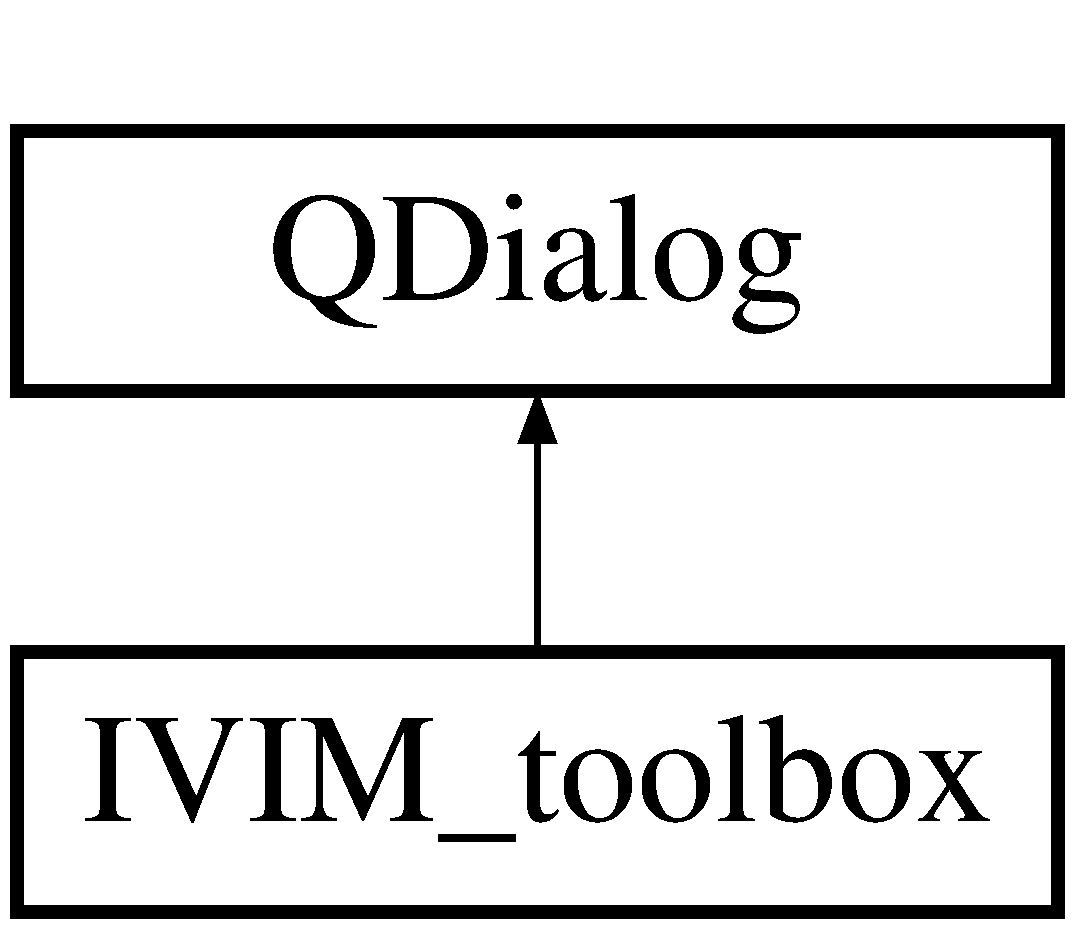
\includegraphics[height=2.000000cm]{classIVIM__toolbox}
\end{center}
\end{figure}
\subsection*{Public Member Functions}
\begin{DoxyCompactItemize}
\item 
\mbox{\Hypertarget{classIVIM__toolbox_a9d85b7349764a673acadb68556b36076}\label{classIVIM__toolbox_a9d85b7349764a673acadb68556b36076}} 
{\bfseries I\+V\+I\+M\+\_\+toolbox} (const Q\+List$<$ \mbox{\hyperlink{classScreen__manager}{Screen\+\_\+manager}} $\ast$$>$ \&\+\_\+sc\+List, Q\+Widget $\ast$parent=0)
\item 
\mbox{\Hypertarget{classIVIM__toolbox_a074ef9f76632c07c62a5d560bfeddbd2}\label{classIVIM__toolbox_a074ef9f76632c07c62a5d560bfeddbd2}} 
{\bfseries I\+V\+I\+M\+\_\+toolbox} (Q\+Widget $\ast$parent=0)
\item 
\mbox{\Hypertarget{classIVIM__toolbox_ab33c4c90b9ffce6b860d3e02f8eb3c5e}\label{classIVIM__toolbox_ab33c4c90b9ffce6b860d3e02f8eb3c5e}} 
void {\bfseries set\+Image\+List} (Q\+List$<$ \mbox{\hyperlink{classScreen__manager}{Screen\+\_\+manager}} $\ast$$>$ \+\_\+list)
\item 
\mbox{\Hypertarget{classIVIM__toolbox_adccace77916a635407425cf9406c99fe}\label{classIVIM__toolbox_adccace77916a635407425cf9406c99fe}} 
bool {\bfseries initialize} ()
\end{DoxyCompactItemize}


The documentation for this class was generated from the following files\+:\begin{DoxyCompactItemize}
\item 
src/tools\+\_\+buildblock/ivim\+\_\+toolbox.\+h\item 
src/tools\+\_\+buildblock/ivim\+\_\+toolbox.\+cpp\end{DoxyCompactItemize}

\hypertarget{classLineTool}{}\section{Line\+Tool Class Reference}
\label{classLineTool}\index{Line\+Tool@{Line\+Tool}}
Inheritance diagram for Line\+Tool\+:\begin{figure}[H]
\begin{center}
\leavevmode
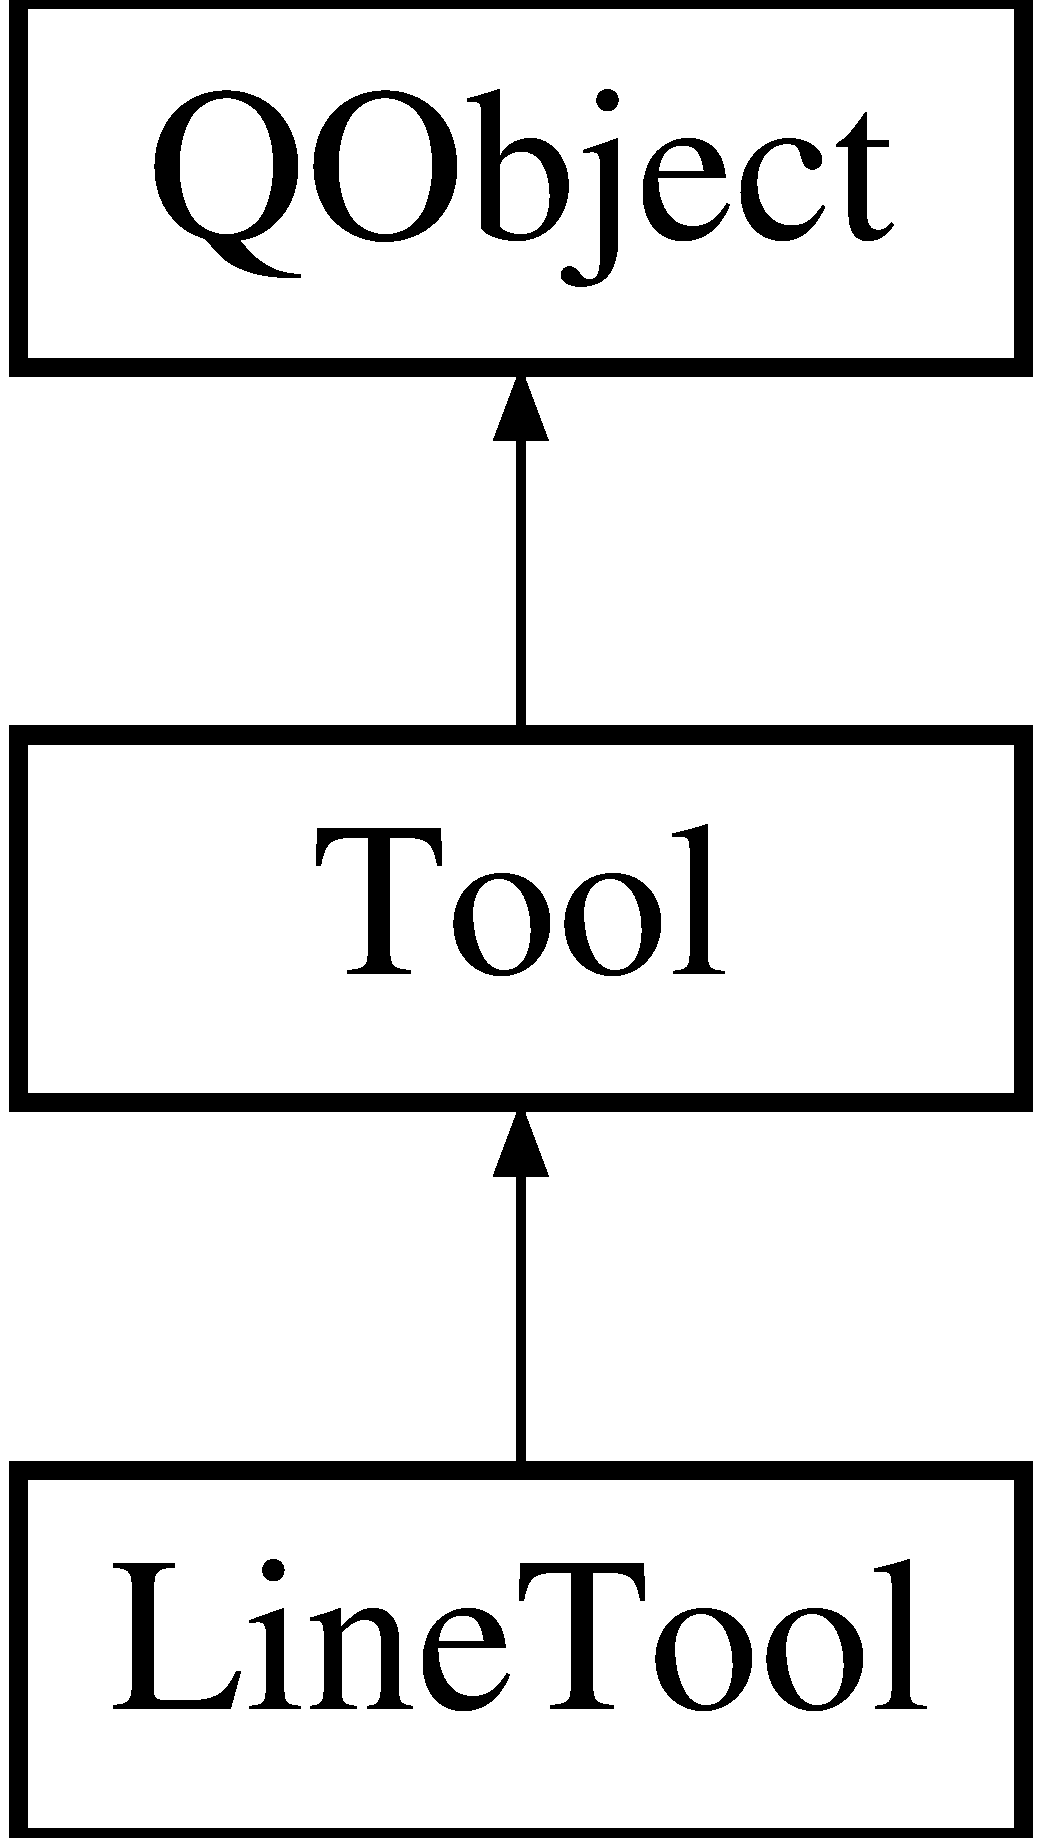
\includegraphics[height=3.000000cm]{classLineTool}
\end{center}
\end{figure}
\subsection*{Signals}
\begin{DoxyCompactItemize}
\item 
\mbox{\Hypertarget{classTool_a68dea3e4c911f3174176084d350865cc}\label{classTool_a68dea3e4c911f3174176084d350865cc}} 
void {\bfseries this\+\_\+selection} (const Q\+Vector$<$ Q\+PointF $>$ \&, Qwt\+Plot $\ast$)
\end{DoxyCompactItemize}
\subsection*{Public Member Functions}
\begin{DoxyCompactItemize}
\item 
\mbox{\Hypertarget{classLineTool_a4816628170735e2a05e2308ac65099e0}\label{classLineTool_a4816628170735e2a05e2308ac65099e0}} 
{\bfseries Line\+Tool} (Q\+Widget $\ast$parent=0)
\item 
\mbox{\Hypertarget{classLineTool_aca8c6283efaa317a1f3327a9e44e2309}\label{classLineTool_aca8c6283efaa317a1f3327a9e44e2309}} 
void {\bfseries set\+Plot} (Qwt\+Plot $\ast$)
\item 
\mbox{\Hypertarget{classLineTool_a00521b226dfd5df9b36d87a439df9a99}\label{classLineTool_a00521b226dfd5df9b36d87a439df9a99}} 
void {\bfseries unset\+Plot} ()
\item 
\mbox{\Hypertarget{classLineTool_a3b1a329dcda63088012e721713049751}\label{classLineTool_a3b1a329dcda63088012e721713049751}} 
virtual void {\bfseries finished\+Selecting} ()
\item 
virtual void \mbox{\hyperlink{classLineTool_a2bcf5d5694e36445607c68c37e4f3f69}{clear\+Before\+Un\+Set}} ()
\item 
\mbox{\Hypertarget{classTool_a020bd5757a03ea7321848a3874f3a8cb}\label{classTool_a020bd5757a03ea7321848a3874f3a8cb}} 
virtual bool {\bfseries event\+Filter} (Q\+Object $\ast$, Q\+Event $\ast$)
\item 
\mbox{\Hypertarget{classTool_aa30c64915020a71d0ea8650e8e966336}\label{classTool_aa30c64915020a71d0ea8650e8e966336}} 
virtual Q\+String {\bfseries get\+\_\+name} () const
\item 
\mbox{\Hypertarget{classTool_a507adfcdafc818d9628b952001b93f3c}\label{classTool_a507adfcdafc818d9628b952001b93f3c}} 
void {\bfseries get\+\_\+data} (Q\+Vector$<$ Q\+PointF $>$ \&, Qwt\+Plot $\ast$)
\end{DoxyCompactItemize}
\subsection*{Protected Member Functions}
\begin{DoxyCompactItemize}
\item 
\mbox{\Hypertarget{classLineTool_a0262637a5a466947883468e740fda29c}\label{classLineTool_a0262637a5a466947883468e740fda29c}} 
void \mbox{\hyperlink{classLineTool_a0262637a5a466947883468e740fda29c}{select}} (const Q\+PointF \&ps)
\begin{DoxyCompactList}\small\item\em On mouse press action. \end{DoxyCompactList}\item 
\mbox{\Hypertarget{classLineTool_a02c8004d82d2f59edf4b685200cd834d}\label{classLineTool_a02c8004d82d2f59edf4b685200cd834d}} 
void \mbox{\hyperlink{classLineTool_a02c8004d82d2f59edf4b685200cd834d}{move}} (const Q\+PointF \&)
\begin{DoxyCompactList}\small\item\em On mouse press and drag action. \end{DoxyCompactList}\item 
\mbox{\Hypertarget{classLineTool_a53f84590f85e08426fe2d6bd39482555}\label{classLineTool_a53f84590f85e08426fe2d6bd39482555}} 
void \mbox{\hyperlink{classLineTool_a53f84590f85e08426fe2d6bd39482555}{clear\+Selection}} ()
\begin{DoxyCompactList}\small\item\em Remove all curves from the c\+\_\+paint\+Device. \end{DoxyCompactList}\item 
\mbox{\Hypertarget{classLineTool_a2a58180a5668ea71ce8411fd39ff5361}\label{classLineTool_a2a58180a5668ea71ce8411fd39ff5361}} 
void {\bfseries update\+Rubber\+Band} ()
\item 
bool \mbox{\hyperlink{classTool_a81244366dc1b9f55465ed6f37b81033c}{check\+Point\+In\+Range}} (const Q\+PointF \&\+\_\+local)
\end{DoxyCompactItemize}
\subsection*{Protected Attributes}
\begin{DoxyCompactItemize}
\item 
\mbox{\Hypertarget{classLineTool_a725a5d5089cb76171ed019a8e1274268}\label{classLineTool_a725a5d5089cb76171ed019a8e1274268}} 
Qwt\+Plot\+Curve $\ast$ {\bfseries curveA}
\item 
\mbox{\Hypertarget{classTool_af0935d8e8edd73d8ec85424b5b15196b}\label{classTool_af0935d8e8edd73d8ec85424b5b15196b}} 
Q\+String {\bfseries name}
\item 
\mbox{\Hypertarget{classTool_a1e301a03c5806c900786760d80049380}\label{classTool_a1e301a03c5806c900786760d80049380}} 
Qwt\+Plot\+Canvas $\ast$ {\bfseries c\+\_\+paint\+Device}
\item 
\mbox{\Hypertarget{classTool_af1d11cc5374ba7eb7c1d41cfb5d4e981}\label{classTool_af1d11cc5374ba7eb7c1d41cfb5d4e981}} 
Qwt\+Plot\+Spectrogram $\ast$ {\bfseries d\+\_\+spectrogram}
\item 
Q\+Vector$<$ Q\+PointF $>$ \mbox{\hyperlink{classTool_a68be77a2e364a7b13d7206388ba5843e}{\+\_\+points}}
\end{DoxyCompactItemize}


\subsection{Member Function Documentation}
\mbox{\Hypertarget{classTool_a81244366dc1b9f55465ed6f37b81033c}\label{classTool_a81244366dc1b9f55465ed6f37b81033c}} 
\index{Line\+Tool@{Line\+Tool}!check\+Point\+In\+Range@{check\+Point\+In\+Range}}
\index{check\+Point\+In\+Range@{check\+Point\+In\+Range}!Line\+Tool@{Line\+Tool}}
\subsubsection{\texorpdfstring{check\+Point\+In\+Range()}{checkPointInRange()}}
{\footnotesize\ttfamily bool Tool\+::check\+Point\+In\+Range (\begin{DoxyParamCaption}\item[{const Q\+PointF \&}]{\+\_\+local }\end{DoxyParamCaption})\hspace{0.3cm}{\ttfamily [protected]}, {\ttfamily [inherited]}}

This is a preliminiry check to see if the point is within the axis range. It has been proven somewhat week condition, as in many cases it fails to provide realible results. \mbox{\Hypertarget{classLineTool_a2bcf5d5694e36445607c68c37e4f3f69}\label{classLineTool_a2bcf5d5694e36445607c68c37e4f3f69}} 
\index{Line\+Tool@{Line\+Tool}!clear\+Before\+Un\+Set@{clear\+Before\+Un\+Set}}
\index{clear\+Before\+Un\+Set@{clear\+Before\+Un\+Set}!Line\+Tool@{Line\+Tool}}
\subsubsection{\texorpdfstring{clear\+Before\+Un\+Set()}{clearBeforeUnSet()}}
{\footnotesize\ttfamily void Line\+Tool\+::clear\+Before\+Un\+Set (\begin{DoxyParamCaption}{ }\end{DoxyParamCaption})\hspace{0.3cm}{\ttfamily [virtual]}}

Cal this function to clean before unsetting a tool. It will try to tight up the screen. 

Implements \mbox{\hyperlink{classTool_a7d9e7d03f4a34d71850cbbfc16ca8532}{Tool}}.



\subsection{Member Data Documentation}
\mbox{\Hypertarget{classTool_a68be77a2e364a7b13d7206388ba5843e}\label{classTool_a68be77a2e364a7b13d7206388ba5843e}} 
\index{Line\+Tool@{Line\+Tool}!\+\_\+points@{\+\_\+points}}
\index{\+\_\+points@{\+\_\+points}!Line\+Tool@{Line\+Tool}}
\subsubsection{\texorpdfstring{\+\_\+points}{\_points}}
{\footnotesize\ttfamily Q\+Vector$<$Q\+PointF$>$ Tool\+::\+\_\+points\hspace{0.3cm}{\ttfamily [protected]}, {\ttfamily [inherited]}}

This vector holds the characteristic points of the selected R\+OI. The \mbox{\hyperlink{classCrossPointerTool}{Cross\+Pointer\+Tool}} has just one point. The \mbox{\hyperlink{classLineTool}{Line\+Tool}} has two points (e.\+g. start and stop) e.\+t.\+c 

The documentation for this class was generated from the following files\+:\begin{DoxyCompactItemize}
\item 
src/tools\+\_\+buildblock/linetool.\+h\item 
src/tools\+\_\+buildblock/linetool.\+cpp\end{DoxyCompactItemize}

\hypertarget{classListROIStat}{}\section{List\+R\+O\+I\+Stat Class Reference}
\label{classListROIStat}\index{List\+R\+O\+I\+Stat@{List\+R\+O\+I\+Stat}}
Inheritance diagram for List\+R\+O\+I\+Stat\+:\begin{figure}[H]
\begin{center}
\leavevmode
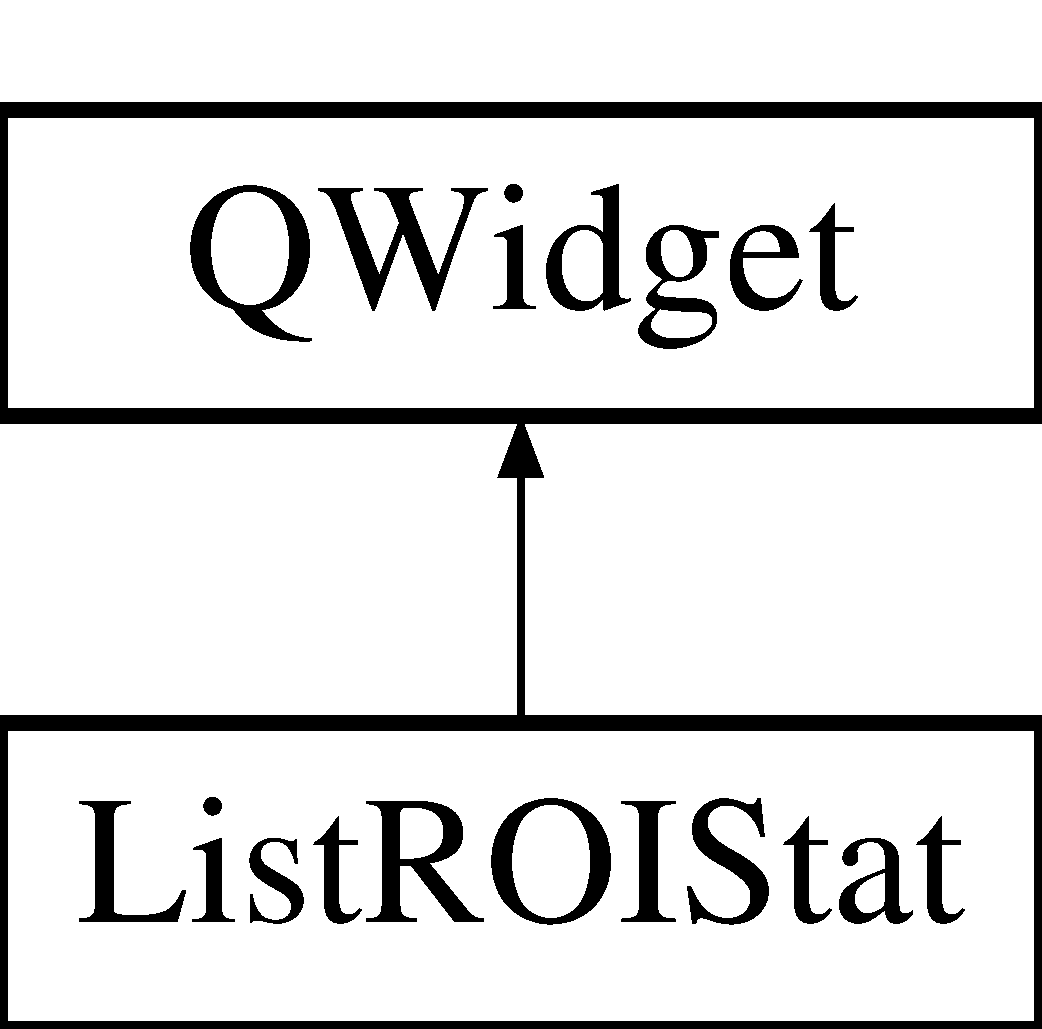
\includegraphics[height=2.000000cm]{classListROIStat}
\end{center}
\end{figure}
\subsection*{Public Member Functions}
\begin{DoxyCompactItemize}
\item 
\mbox{\Hypertarget{classListROIStat_ab75dfecc931323b639ba32dbf2e557ee}\label{classListROIStat_ab75dfecc931323b639ba32dbf2e557ee}} 
{\bfseries List\+R\+O\+I\+Stat} (Q\+Widget $\ast$parent=0)
\item 
\mbox{\Hypertarget{classListROIStat_af4dcd07465031df2bde1bfeda358e8d4}\label{classListROIStat_af4dcd07465031df2bde1bfeda358e8d4}} 
bool {\bfseries analyse\+All} (const stir\+::\+Pixels\+On\+Cartesian\+Grid$<$ float $>$ \&\+\_\+w)
\item 
\mbox{\Hypertarget{classListROIStat_a984e01f7cb3fae2752f89ebdf51523f2}\label{classListROIStat_a984e01f7cb3fae2752f89ebdf51523f2}} 
void {\bfseries set\+Data} (const stir\+::\+Pixels\+On\+Cartesian\+Grid$<$ float $>$ \&\+\_\+w)
\item 
\mbox{\Hypertarget{classListROIStat_a73c43119352ccf1d60a29f4ea79b1601}\label{classListROIStat_a73c43119352ccf1d60a29f4ea79b1601}} 
void {\bfseries un\+Set\+Data} ()
\item 
\mbox{\Hypertarget{classListROIStat_a3987566eb4dd9b25aaadcd9cbf323049}\label{classListROIStat_a3987566eb4dd9b25aaadcd9cbf323049}} 
float {\bfseries get\+Area} (const stir\+::\+Pixels\+On\+Cartesian\+Grid$<$ float $>$ \&\+\_\+w)
\item 
\mbox{\Hypertarget{classListROIStat_ab293143fbff73460757fe27e59fca768}\label{classListROIStat_ab293143fbff73460757fe27e59fca768}} 
float {\bfseries get\+Mean} (const stir\+::\+Pixels\+On\+Cartesian\+Grid$<$ float $>$ \&\+\_\+w)
\item 
\mbox{\Hypertarget{classListROIStat_a2adc70755e4fec8874ec0198dfb9ac55}\label{classListROIStat_a2adc70755e4fec8874ec0198dfb9ac55}} 
float {\bfseries get\+SD} (const stir\+::\+Pixels\+On\+Cartesian\+Grid$<$ float $>$ \&\+\_\+w)
\end{DoxyCompactItemize}


The documentation for this class was generated from the following files\+:\begin{DoxyCompactItemize}
\item 
src/display\+\_\+buildblock/listroistat.\+h\item 
src/display\+\_\+buildblock/listroistat.\+cpp\end{DoxyCompactItemize}

\hypertarget{classMainWindow}{}\section{Main\+Window Class Reference}
\label{classMainWindow}\index{Main\+Window@{Main\+Window}}


The \mbox{\hyperlink{classMainWindow}{Main\+Window}} class The main window class has all the managerial responsibilities in the application. It handles the main G\+UI and the actions between the displayed objects.  




{\ttfamily \#include $<$mainwindow.\+h$>$}

Inheritance diagram for Main\+Window\+:\begin{figure}[H]
\begin{center}
\leavevmode
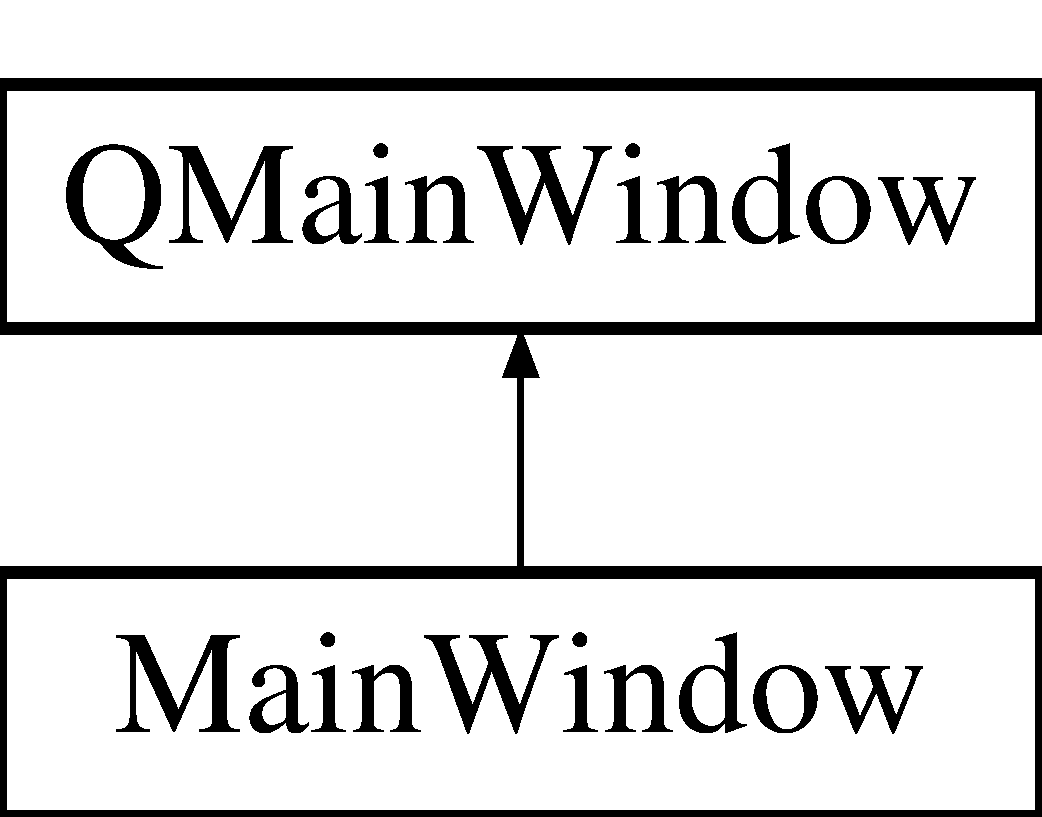
\includegraphics[height=2.000000cm]{classMainWindow}
\end{center}
\end{figure}
\subsection*{Public Slots}
\begin{DoxyCompactItemize}
\item 
\mbox{\Hypertarget{classMainWindow_a045c3743032b6a84784279d4c9d9bd77}\label{classMainWindow_a045c3743032b6a84784279d4c9d9bd77}} 
void {\bfseries set\+\_\+tool} (std\+::shared\+\_\+ptr$<$ \mbox{\hyperlink{classTool}{Tool}} $>$)
\end{DoxyCompactItemize}
\subsection*{Signals}
\begin{DoxyCompactItemize}
\item 
\mbox{\Hypertarget{classMainWindow_aad224a9b6fa5706eb6bc5bea8ad0ce86}\label{classMainWindow_aad224a9b6fa5706eb6bc5bea8ad0ce86}} 
void {\bfseries sub\+Window\+Ready} (Q\+Widget $\ast$)
\end{DoxyCompactItemize}
\subsection*{Public Member Functions}
\begin{DoxyCompactItemize}
\item 
\mbox{\Hypertarget{classMainWindow_a8b244be8b7b7db1b08de2a2acb9409db}\label{classMainWindow_a8b244be8b7b7db1b08de2a2acb9409db}} 
{\bfseries Main\+Window} (Q\+Widget $\ast$parent=0)
\end{DoxyCompactItemize}
\subsection*{Protected Member Functions}
\begin{DoxyCompactItemize}
\item 
\mbox{\Hypertarget{classMainWindow_a05fb9d72c044aa3bb7d187b994704e2f}\label{classMainWindow_a05fb9d72c044aa3bb7d187b994704e2f}} 
void {\bfseries close\+Event} (Q\+Close\+Event $\ast$event) override
\end{DoxyCompactItemize}


\subsection{Detailed Description}
The \mbox{\hyperlink{classMainWindow}{Main\+Window}} class The main window class has all the managerial responsibilities in the application. It handles the main G\+UI and the actions between the displayed objects. 

The documentation for this class was generated from the following files\+:\begin{DoxyCompactItemize}
\item 
src/ui\+\_\+buildblock/mainwindow.\+h\item 
src/ui\+\_\+buildblock/mainwindow.\+cpp\end{DoxyCompactItemize}

\hypertarget{classViewer_1_1Mapper}{}\section{Viewer\+:\+:Mapper Class Reference}
\label{classViewer_1_1Mapper}\index{Viewer\+::\+Mapper@{Viewer\+::\+Mapper}}
\subsection*{Static Public Member Functions}
\begin{DoxyCompactItemize}
\item 
\mbox{\Hypertarget{classViewer_1_1Mapper_ad0a5be908ffe8bb35fdff76ffe58c06f}\label{classViewer_1_1Mapper_ad0a5be908ffe8bb35fdff76ffe58c06f}} 
static Q\+Vector$<$ float $>$ {\bfseries from} (const stir\+::\+Array$<$ 2, float $>$ \&input)
\item 
\mbox{\Hypertarget{classViewer_1_1Mapper_a971705ae10598e69634e11b9f677e0a1}\label{classViewer_1_1Mapper_a971705ae10598e69634e11b9f677e0a1}} 
{\footnotesize template$<$int num\+\_\+dimensions$>$ }\\static stir\+::\+Array$<$ num\+\_\+dimensions, float $>$ {\bfseries from} (const Q\+Vector$<$ float $>$ \&input, const stir\+::\+Index\+Range$<$ num\+\_\+dimensions $>$ \&ranges)
\item 
\mbox{\Hypertarget{classViewer_1_1Mapper_a3fb2e58c9ada63d8c173499b173d0715}\label{classViewer_1_1Mapper_a3fb2e58c9ada63d8c173499b173d0715}} 
static Q\+Vector$<$ float $>$ {\bfseries from} (const stir\+::\+Voxels\+On\+Cartesian\+Grid$<$ float $>$ \&input)
\item 
\mbox{\Hypertarget{classViewer_1_1Mapper_a11ff9d51a899599171e4470949deb703}\label{classViewer_1_1Mapper_a11ff9d51a899599171e4470949deb703}} 
static stir\+::\+Voxels\+On\+Cartesian\+Grid$<$ float $>$ {\bfseries from} (const Q\+Vector$<$ float $>$ \&input, const stir\+::\+Cartesian\+Coordinate3D$<$ float $>$ \&origin, const stir\+::\+Basic\+Coordinate$<$ 3, float $>$ \&grid\+\_\+spacing)
\end{DoxyCompactItemize}


The documentation for this class was generated from the following file\+:\begin{DoxyCompactItemize}
\item 
src/buildblock/common.\+h\end{DoxyCompactItemize}

\hypertarget{classmyQListWidgetItem}{}\section{my\+Q\+List\+Widget\+Item Class Reference}
\label{classmyQListWidgetItem}\index{my\+Q\+List\+Widget\+Item@{my\+Q\+List\+Widget\+Item}}
Inheritance diagram for my\+Q\+List\+Widget\+Item\+:\begin{figure}[H]
\begin{center}
\leavevmode
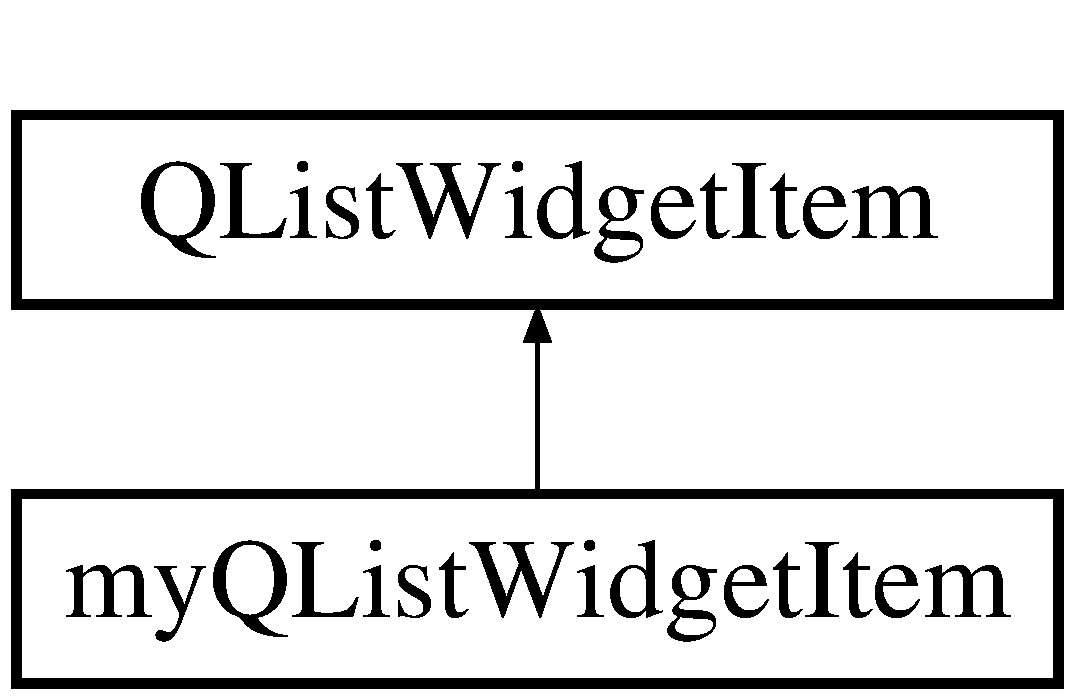
\includegraphics[height=2.000000cm]{classmyQListWidgetItem}
\end{center}
\end{figure}
\subsection*{Public Member Functions}
\begin{DoxyCompactItemize}
\item 
\mbox{\Hypertarget{classmyQListWidgetItem_ad4ae475527f8e96cd41a2f2e91fddd99}\label{classmyQListWidgetItem_ad4ae475527f8e96cd41a2f2e91fddd99}} 
void {\bfseries set\+\_\+mdi\+Window\+\_\+ptr} (\mbox{\hyperlink{classScreen__manager}{Screen\+\_\+manager}} $\ast$new\+\_\+screen)
\item 
\mbox{\Hypertarget{classmyQListWidgetItem_a33ca8234a762bc4f8b7114228d0ea2f3}\label{classmyQListWidgetItem_a33ca8234a762bc4f8b7114228d0ea2f3}} 
\mbox{\hyperlink{classScreen__manager}{Screen\+\_\+manager}} $\ast$ {\bfseries get\+\_\+mdi\+Window\+\_\+ptr} () const
\end{DoxyCompactItemize}


The documentation for this class was generated from the following files\+:\begin{DoxyCompactItemize}
\item 
src/ui\+\_\+buildblock/myqlistwidgetitem.\+h\item 
src/ui\+\_\+buildblock/myqlistwidgetitem.\+cpp\end{DoxyCompactItemize}

\hypertarget{classp__data}{}\section{p\+\_\+data Class Reference}
\label{classp__data}\index{p\+\_\+data@{p\+\_\+data}}
\subsection*{Public Member Functions}
\begin{DoxyCompactItemize}
\item 
\mbox{\Hypertarget{classp__data_afe078d5fada14791138de11cc25e6332}\label{classp__data_afe078d5fada14791138de11cc25e6332}} 
{\bfseries p\+\_\+data} (const \mbox{\hyperlink{classViewer_1_1SimpleVector3D}{Viewer\+::\+Simple\+Vector3D}}$<$ int $>$ \&\+\_\+v, const float \&\+\_\+f)
\end{DoxyCompactItemize}
\subsection*{Public Attributes}
\begin{DoxyCompactItemize}
\item 
\mbox{\Hypertarget{classp__data_a74086cad872722b4c6a65d665835c590}\label{classp__data_a74086cad872722b4c6a65d665835c590}} 
\mbox{\hyperlink{classViewer_1_1SimpleVector3D}{Viewer\+::\+Simple\+Vector3D}}$<$ int $>$ {\bfseries cur\+\_\+pos}
\item 
\mbox{\Hypertarget{classp__data_a24d69b3ec7f90e7b2f812f4340130c27}\label{classp__data_a24d69b3ec7f90e7b2f812f4340130c27}} 
float {\bfseries cur\+\_\+value}
\end{DoxyCompactItemize}


The documentation for this class was generated from the following file\+:\begin{DoxyCompactItemize}
\item 
src/ui\+\_\+buildblock/panel\+\_\+cross\+\_\+pointer.\+h\end{DoxyCompactItemize}

\hypertarget{classpanel__cross__pointer}{}\section{panel\+\_\+cross\+\_\+pointer Class Reference}
\label{classpanel__cross__pointer}\index{panel\+\_\+cross\+\_\+pointer@{panel\+\_\+cross\+\_\+pointer}}
Inheritance diagram for panel\+\_\+cross\+\_\+pointer\+:\begin{figure}[H]
\begin{center}
\leavevmode
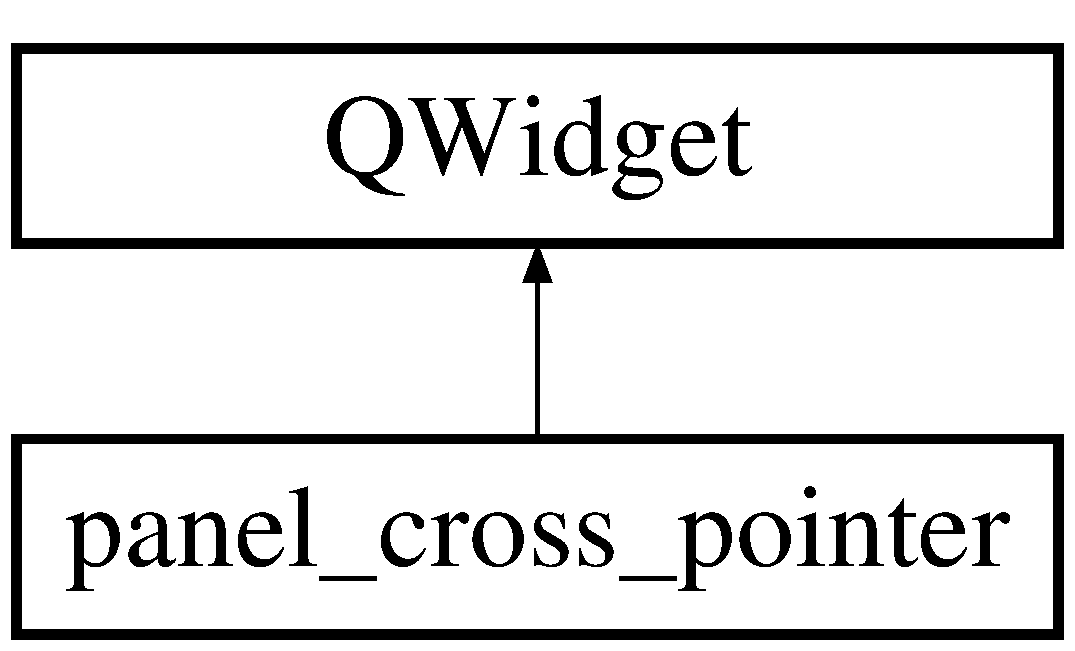
\includegraphics[height=2.000000cm]{classpanel__cross__pointer}
\end{center}
\end{figure}
\subsection*{Public Slots}
\begin{DoxyCompactItemize}
\item 
\mbox{\Hypertarget{classpanel__cross__pointer_a03403c4e7e2be4f368865ce2ec1542b7}\label{classpanel__cross__pointer_a03403c4e7e2be4f368865ce2ec1542b7}} 
void {\bfseries print\+\_\+point} (const \mbox{\hyperlink{classViewer_1_1SimpleVector3D}{Viewer\+::\+Simple\+Vector3D}}$<$ int $>$ \&ps, const double \&\+\_\+v)
\end{DoxyCompactItemize}
\subsection*{Signals}
\begin{DoxyCompactItemize}
\item 
\mbox{\Hypertarget{classpanel__cross__pointer_a8fefaeafa3c834de0e876c4c6ebd5867}\label{classpanel__cross__pointer_a8fefaeafa3c834de0e876c4c6ebd5867}} 
void {\bfseries select\+\_\+this\+\_\+point} (const \mbox{\hyperlink{classViewer_1_1SimpleVector3D}{Viewer\+::\+Simple\+Vector3D}}$<$ int $>$ \&)
\end{DoxyCompactItemize}
\subsection*{Public Member Functions}
\begin{DoxyCompactItemize}
\item 
\mbox{\Hypertarget{classpanel__cross__pointer_a362b714054b0baa955d11a40b17edf7c}\label{classpanel__cross__pointer_a362b714054b0baa955d11a40b17edf7c}} 
{\bfseries panel\+\_\+cross\+\_\+pointer} (Q\+Widget $\ast$parent=0)
\end{DoxyCompactItemize}


The documentation for this class was generated from the following files\+:\begin{DoxyCompactItemize}
\item 
src/ui\+\_\+buildblock/panel\+\_\+cross\+\_\+pointer.\+h\item 
src/ui\+\_\+buildblock/panel\+\_\+cross\+\_\+pointer.\+cpp\end{DoxyCompactItemize}

\hypertarget{classPanelLinePointer}{}\section{Panel\+Line\+Pointer Class Reference}
\label{classPanelLinePointer}\index{Panel\+Line\+Pointer@{Panel\+Line\+Pointer}}
Inheritance diagram for Panel\+Line\+Pointer\+:\begin{figure}[H]
\begin{center}
\leavevmode
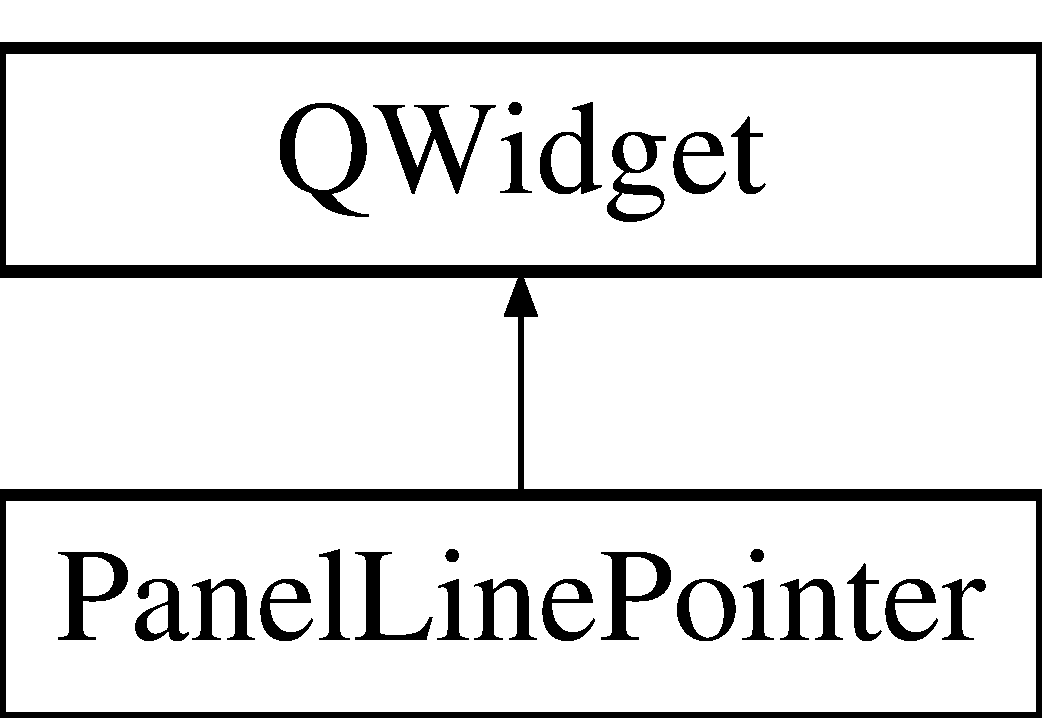
\includegraphics[height=2.000000cm]{classPanelLinePointer}
\end{center}
\end{figure}
\subsection*{Signals}
\begin{DoxyCompactItemize}
\item 
\mbox{\Hypertarget{classPanelLinePointer_aa7fd10395dca3172441d8f131670d014}\label{classPanelLinePointer_aa7fd10395dca3172441d8f131670d014}} 
void {\bfseries new\+\_\+options} ()
\end{DoxyCompactItemize}
\subsection*{Public Member Functions}
\begin{DoxyCompactItemize}
\item 
\mbox{\Hypertarget{classPanelLinePointer_a450331ef5c7d4bab97d341d0175d4c5c}\label{classPanelLinePointer_a450331ef5c7d4bab97d341d0175d4c5c}} 
{\bfseries Panel\+Line\+Pointer} (Q\+Widget $\ast$parent=0)
\item 
\mbox{\Hypertarget{classPanelLinePointer_a8f3fabdf4ead8d94ed1dee4aa5fe202e}\label{classPanelLinePointer_a8f3fabdf4ead8d94ed1dee4aa5fe202e}} 
int \mbox{\hyperlink{classPanelLinePointer_a8f3fabdf4ead8d94ed1dee4aa5fe202e}{get\+Num\+Rays}} () const
\begin{DoxyCompactList}\small\item\em Return the number of rays to be used. \end{DoxyCompactList}\item 
\mbox{\Hypertarget{classPanelLinePointer_a0a7d3adc7d8a04c3fcce25e5449d9506}\label{classPanelLinePointer_a0a7d3adc7d8a04c3fcce25e5449d9506}} 
bool {\bfseries get\+Fidelity} () const
\item 
\mbox{\Hypertarget{classPanelLinePointer_a5ed7cf8f59bae287d75b6eba99d95334}\label{classPanelLinePointer_a5ed7cf8f59bae287d75b6eba99d95334}} 
bool {\bfseries get\+Draw\+Pixels} () const
\item 
\mbox{\Hypertarget{classPanelLinePointer_a618ef022ec836d9fdbd0def1269b35ff}\label{classPanelLinePointer_a618ef022ec836d9fdbd0def1269b35ff}} 
bool {\bfseries get\+Antialiazing} () const
\end{DoxyCompactItemize}


The documentation for this class was generated from the following files\+:\begin{DoxyCompactItemize}
\item 
src/ui\+\_\+buildblock/panellinepointer.\+h\item 
src/ui\+\_\+buildblock/panellinepointer.\+cpp\end{DoxyCompactItemize}

\hypertarget{classPanelRectPointer}{}\section{Panel\+Rect\+Pointer Class Reference}
\label{classPanelRectPointer}\index{Panel\+Rect\+Pointer@{Panel\+Rect\+Pointer}}
Inheritance diagram for Panel\+Rect\+Pointer\+:\begin{figure}[H]
\begin{center}
\leavevmode
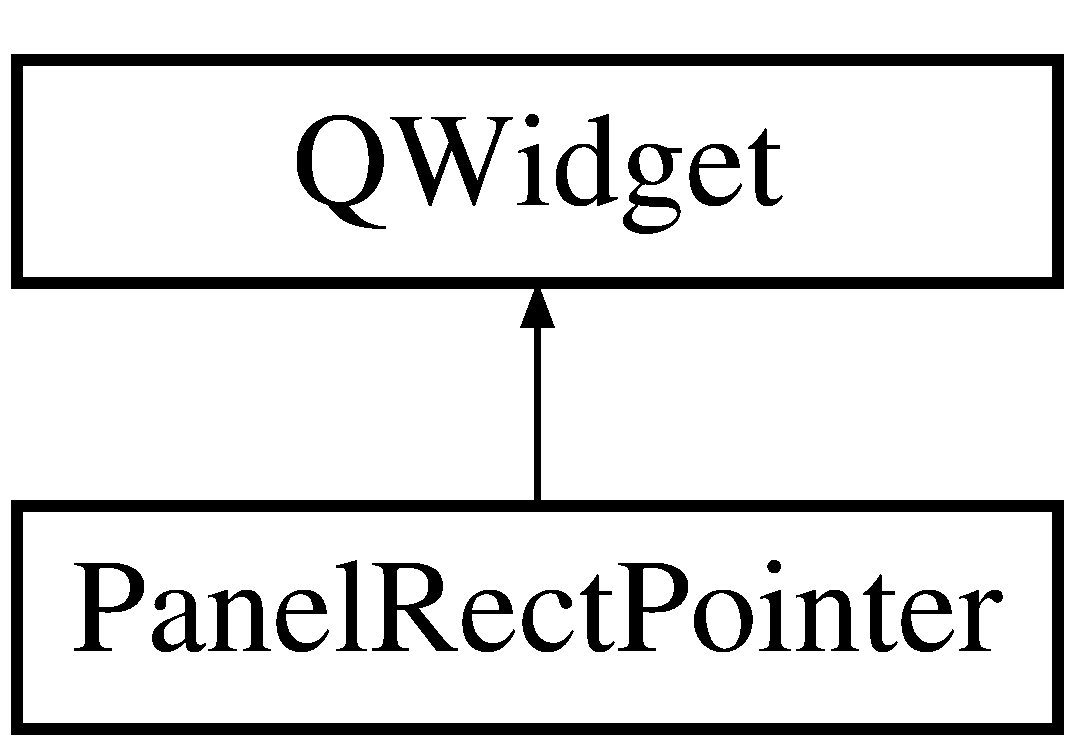
\includegraphics[height=2.000000cm]{classPanelRectPointer}
\end{center}
\end{figure}
\subsection*{Public Member Functions}
\begin{DoxyCompactItemize}
\item 
\mbox{\Hypertarget{classPanelRectPointer_ab676f08ddc72852f5c02bd1b8be92282}\label{classPanelRectPointer_ab676f08ddc72852f5c02bd1b8be92282}} 
{\bfseries Panel\+Rect\+Pointer} (Q\+Widget $\ast$parent=0)
\end{DoxyCompactItemize}


The documentation for this class was generated from the following files\+:\begin{DoxyCompactItemize}
\item 
src/ui\+\_\+buildblock/panelrectpointer.\+h\item 
src/ui\+\_\+buildblock/panelrectpointer.\+cpp\end{DoxyCompactItemize}

\hypertarget{classPointerTool}{}\section{Pointer\+Tool Class Reference}
\label{classPointerTool}\index{Pointer\+Tool@{Pointer\+Tool}}
Inheritance diagram for Pointer\+Tool\+:\begin{figure}[H]
\begin{center}
\leavevmode
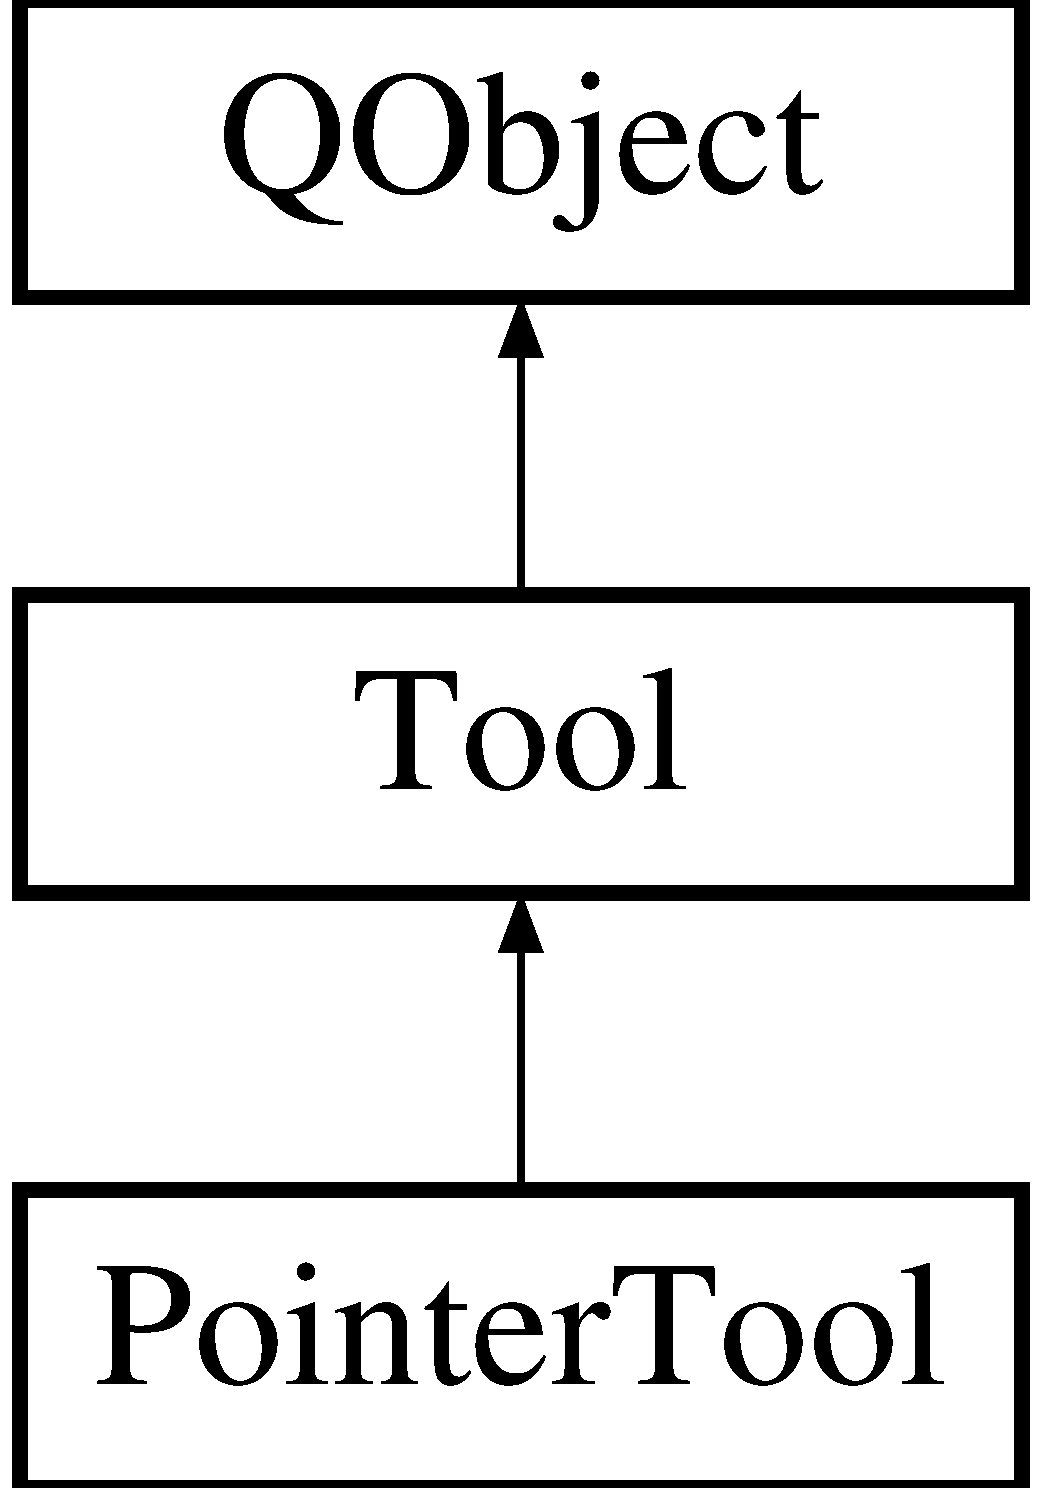
\includegraphics[height=3.000000cm]{classPointerTool}
\end{center}
\end{figure}
\subsection*{Signals}
\begin{DoxyCompactItemize}
\item 
\mbox{\Hypertarget{classTool_a68dea3e4c911f3174176084d350865cc}\label{classTool_a68dea3e4c911f3174176084d350865cc}} 
void {\bfseries this\+\_\+selection} (const Q\+Vector$<$ Q\+PointF $>$ \&, Qwt\+Plot $\ast$)
\end{DoxyCompactItemize}
\subsection*{Public Member Functions}
\begin{DoxyCompactItemize}
\item 
\mbox{\Hypertarget{classPointerTool_ad40ae55e67021175db7b749a163f428b}\label{classPointerTool_ad40ae55e67021175db7b749a163f428b}} 
{\bfseries Pointer\+Tool} (Q\+Widget $\ast$parent=0)
\item 
\mbox{\Hypertarget{classPointerTool_a66ba22cda0710f26e84fac942157c316}\label{classPointerTool_a66ba22cda0710f26e84fac942157c316}} 
void {\bfseries set\+\_\+size} (const float \&, const float \&)
\item 
\mbox{\Hypertarget{classPointerTool_a44797227fc09fff30a4ac7ab1e38ef82}\label{classPointerTool_a44797227fc09fff30a4ac7ab1e38ef82}} 
void {\bfseries set\+\_\+width} (const float \&)
\item 
\mbox{\Hypertarget{classPointerTool_ad069a930adfd400c9802366f2f270422}\label{classPointerTool_ad069a930adfd400c9802366f2f270422}} 
void {\bfseries set\+\_\+height} (const float \&)
\item 
\mbox{\Hypertarget{classPointerTool_a96e38dd0c6beb7cc4f33b031e311f6d6}\label{classPointerTool_a96e38dd0c6beb7cc4f33b031e311f6d6}} 
void {\bfseries set\+Plot} (Qwt\+Plot $\ast$)
\item 
\mbox{\Hypertarget{classPointerTool_acec8781a7d4b55c143d2047a40c88ff9}\label{classPointerTool_acec8781a7d4b55c143d2047a40c88ff9}} 
virtual void {\bfseries finished\+Selecting} ()
\item 
virtual void \mbox{\hyperlink{classPointerTool_a04c325128dc9ee27272eace9e70d15aa}{clear\+Before\+Un\+Set}} ()
\item 
\mbox{\Hypertarget{classTool_a020bd5757a03ea7321848a3874f3a8cb}\label{classTool_a020bd5757a03ea7321848a3874f3a8cb}} 
virtual bool {\bfseries event\+Filter} (Q\+Object $\ast$, Q\+Event $\ast$)
\item 
\mbox{\Hypertarget{classTool_aa30c64915020a71d0ea8650e8e966336}\label{classTool_aa30c64915020a71d0ea8650e8e966336}} 
virtual Q\+String {\bfseries get\+\_\+name} () const
\item 
\mbox{\Hypertarget{classTool_a507adfcdafc818d9628b952001b93f3c}\label{classTool_a507adfcdafc818d9628b952001b93f3c}} 
void {\bfseries get\+\_\+data} (Q\+Vector$<$ Q\+PointF $>$ \&, Qwt\+Plot $\ast$)
\end{DoxyCompactItemize}
\subsection*{Protected Member Functions}
\begin{DoxyCompactItemize}
\item 
\mbox{\Hypertarget{classPointerTool_a976caf364c090420e3b21b7b029f6f13}\label{classPointerTool_a976caf364c090420e3b21b7b029f6f13}} 
void \mbox{\hyperlink{classPointerTool_a976caf364c090420e3b21b7b029f6f13}{select}} (const Q\+PointF \&)
\begin{DoxyCompactList}\small\item\em On mouse press action. \end{DoxyCompactList}\item 
\mbox{\Hypertarget{classPointerTool_a56e94e4962b110df07eb8925131e2c0e}\label{classPointerTool_a56e94e4962b110df07eb8925131e2c0e}} 
void \mbox{\hyperlink{classPointerTool_a56e94e4962b110df07eb8925131e2c0e}{move}} (const Q\+PointF \&)
\begin{DoxyCompactList}\small\item\em On mouse press and drag action. \end{DoxyCompactList}\item 
\mbox{\Hypertarget{classTool_a11f1da4092d196a7b91d3d60276586eb}\label{classTool_a11f1da4092d196a7b91d3d60276586eb}} 
virtual void \mbox{\hyperlink{classTool_a11f1da4092d196a7b91d3d60276586eb}{clear\+Selection}} ()
\begin{DoxyCompactList}\small\item\em Remove all curves from the c\+\_\+paint\+Device. \end{DoxyCompactList}\item 
bool \mbox{\hyperlink{classTool_a81244366dc1b9f55465ed6f37b81033c}{check\+Point\+In\+Range}} (const Q\+PointF \&\+\_\+local)
\end{DoxyCompactItemize}
\subsection*{Protected Attributes}
\begin{DoxyCompactItemize}
\item 
\mbox{\Hypertarget{classTool_af0935d8e8edd73d8ec85424b5b15196b}\label{classTool_af0935d8e8edd73d8ec85424b5b15196b}} 
Q\+String {\bfseries name}
\item 
\mbox{\Hypertarget{classTool_a1e301a03c5806c900786760d80049380}\label{classTool_a1e301a03c5806c900786760d80049380}} 
Qwt\+Plot\+Canvas $\ast$ {\bfseries c\+\_\+paint\+Device}
\item 
\mbox{\Hypertarget{classTool_af1d11cc5374ba7eb7c1d41cfb5d4e981}\label{classTool_af1d11cc5374ba7eb7c1d41cfb5d4e981}} 
Qwt\+Plot\+Spectrogram $\ast$ {\bfseries d\+\_\+spectrogram}
\item 
Q\+Vector$<$ Q\+PointF $>$ \mbox{\hyperlink{classTool_a68be77a2e364a7b13d7206388ba5843e}{\+\_\+points}}
\end{DoxyCompactItemize}


\subsection{Member Function Documentation}
\mbox{\Hypertarget{classTool_a81244366dc1b9f55465ed6f37b81033c}\label{classTool_a81244366dc1b9f55465ed6f37b81033c}} 
\index{Pointer\+Tool@{Pointer\+Tool}!check\+Point\+In\+Range@{check\+Point\+In\+Range}}
\index{check\+Point\+In\+Range@{check\+Point\+In\+Range}!Pointer\+Tool@{Pointer\+Tool}}
\subsubsection{\texorpdfstring{check\+Point\+In\+Range()}{checkPointInRange()}}
{\footnotesize\ttfamily bool Tool\+::check\+Point\+In\+Range (\begin{DoxyParamCaption}\item[{const Q\+PointF \&}]{\+\_\+local }\end{DoxyParamCaption})\hspace{0.3cm}{\ttfamily [protected]}, {\ttfamily [inherited]}}

This is a preliminiry check to see if the point is within the axis range. It has been proven somewhat week condition, as in many cases it fails to provide realible results. \mbox{\Hypertarget{classPointerTool_a04c325128dc9ee27272eace9e70d15aa}\label{classPointerTool_a04c325128dc9ee27272eace9e70d15aa}} 
\index{Pointer\+Tool@{Pointer\+Tool}!clear\+Before\+Un\+Set@{clear\+Before\+Un\+Set}}
\index{clear\+Before\+Un\+Set@{clear\+Before\+Un\+Set}!Pointer\+Tool@{Pointer\+Tool}}
\subsubsection{\texorpdfstring{clear\+Before\+Un\+Set()}{clearBeforeUnSet()}}
{\footnotesize\ttfamily void Pointer\+Tool\+::clear\+Before\+Un\+Set (\begin{DoxyParamCaption}{ }\end{DoxyParamCaption})\hspace{0.3cm}{\ttfamily [virtual]}}

Cal this function to clean before unsetting a tool. It will try to tight up the screen. 

Implements \mbox{\hyperlink{classTool_a7d9e7d03f4a34d71850cbbfc16ca8532}{Tool}}.



\subsection{Member Data Documentation}
\mbox{\Hypertarget{classTool_a68be77a2e364a7b13d7206388ba5843e}\label{classTool_a68be77a2e364a7b13d7206388ba5843e}} 
\index{Pointer\+Tool@{Pointer\+Tool}!\+\_\+points@{\+\_\+points}}
\index{\+\_\+points@{\+\_\+points}!Pointer\+Tool@{Pointer\+Tool}}
\subsubsection{\texorpdfstring{\+\_\+points}{\_points}}
{\footnotesize\ttfamily Q\+Vector$<$Q\+PointF$>$ Tool\+::\+\_\+points\hspace{0.3cm}{\ttfamily [protected]}, {\ttfamily [inherited]}}

This vector holds the characteristic points of the selected R\+OI. The \mbox{\hyperlink{classCrossPointerTool}{Cross\+Pointer\+Tool}} has just one point. The \mbox{\hyperlink{classLineTool}{Line\+Tool}} has two points (e.\+g. start and stop) e.\+t.\+c 

The documentation for this class was generated from the following files\+:\begin{DoxyCompactItemize}
\item 
src/tools\+\_\+buildblock/pointertool.\+h\item 
src/tools\+\_\+buildblock/pointertool.\+cpp\end{DoxyCompactItemize}

\hypertarget{classRectTool}{}\section{Rect\+Tool Class Reference}
\label{classRectTool}\index{Rect\+Tool@{Rect\+Tool}}
Inheritance diagram for Rect\+Tool\+:\begin{figure}[H]
\begin{center}
\leavevmode
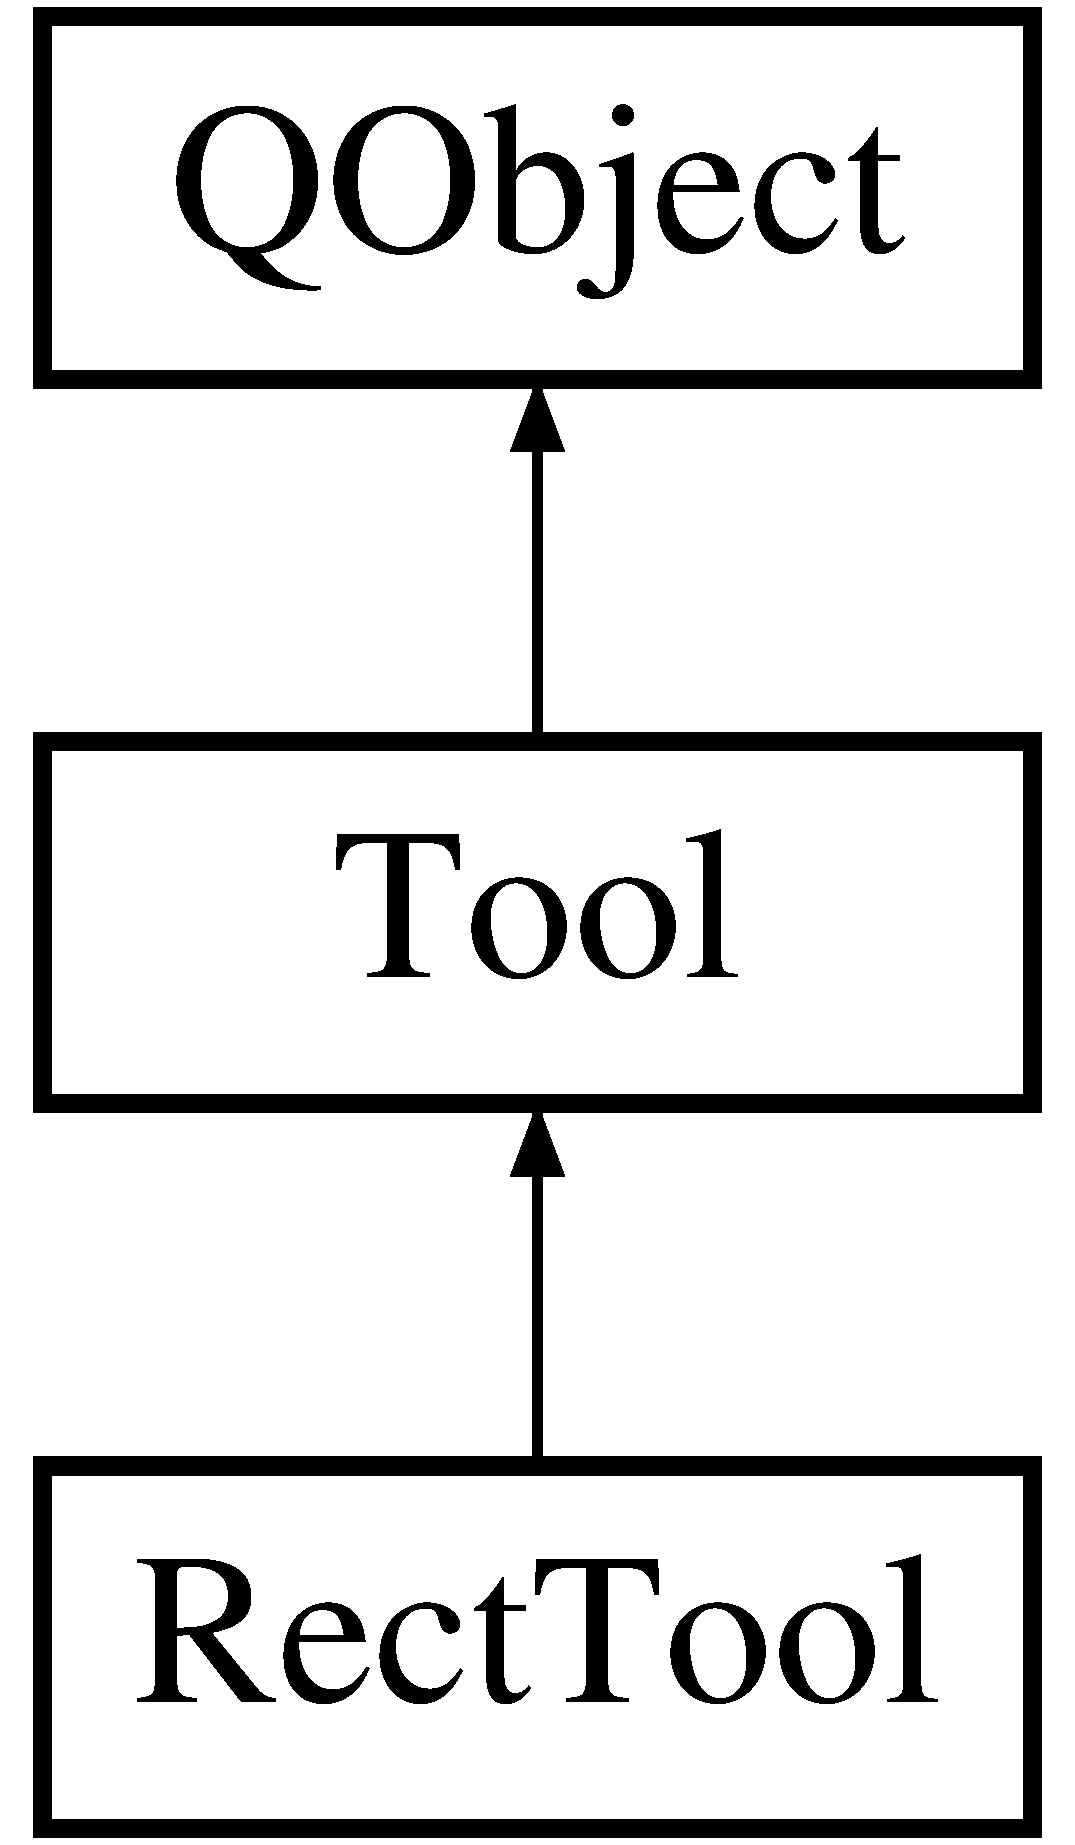
\includegraphics[height=3.000000cm]{classRectTool}
\end{center}
\end{figure}
\subsection*{Public Slots}
\begin{DoxyCompactItemize}
\item 
\mbox{\Hypertarget{classRectTool_a3a2b0b9e208c876e08588378fe90aac4}\label{classRectTool_a3a2b0b9e208c876e08588378fe90aac4}} 
void {\bfseries new\+\_\+\+Selection} (const Q\+RectF \&points)
\end{DoxyCompactItemize}
\subsection*{Signals}
\begin{DoxyCompactItemize}
\item 
\mbox{\Hypertarget{classTool_a68dea3e4c911f3174176084d350865cc}\label{classTool_a68dea3e4c911f3174176084d350865cc}} 
void {\bfseries this\+\_\+selection} (const Q\+Vector$<$ Q\+PointF $>$ \&, Qwt\+Plot $\ast$)
\end{DoxyCompactItemize}
\subsection*{Public Member Functions}
\begin{DoxyCompactItemize}
\item 
\mbox{\Hypertarget{classRectTool_aa2ec592743f5be9366620cfcd76ac91a}\label{classRectTool_aa2ec592743f5be9366620cfcd76ac91a}} 
{\bfseries Rect\+Tool} (Q\+Widget $\ast$parent=0)
\item 
\mbox{\Hypertarget{classRectTool_a0061642e759546f6dcd7c1a2c3b96393}\label{classRectTool_a0061642e759546f6dcd7c1a2c3b96393}} 
void {\bfseries set\+Plot} (Qwt\+Plot $\ast$)
\item 
\mbox{\Hypertarget{classRectTool_a08ce587da86dc1b8335cb265bb2a3efd}\label{classRectTool_a08ce587da86dc1b8335cb265bb2a3efd}} 
void {\bfseries unset\+Plot} ()
\item 
\mbox{\Hypertarget{classRectTool_a1ce7bea2dcb7d122be6fd342720c986c}\label{classRectTool_a1ce7bea2dcb7d122be6fd342720c986c}} 
virtual void {\bfseries finished\+Selecting} ()
\item 
virtual void \mbox{\hyperlink{classRectTool_a22ddb88797de61ed921a5cd3462383ea}{clear\+Before\+Un\+Set}} ()
\item 
\mbox{\Hypertarget{classTool_a020bd5757a03ea7321848a3874f3a8cb}\label{classTool_a020bd5757a03ea7321848a3874f3a8cb}} 
virtual bool {\bfseries event\+Filter} (Q\+Object $\ast$, Q\+Event $\ast$)
\item 
\mbox{\Hypertarget{classTool_aa30c64915020a71d0ea8650e8e966336}\label{classTool_aa30c64915020a71d0ea8650e8e966336}} 
virtual Q\+String {\bfseries get\+\_\+name} () const
\item 
\mbox{\Hypertarget{classTool_a507adfcdafc818d9628b952001b93f3c}\label{classTool_a507adfcdafc818d9628b952001b93f3c}} 
void {\bfseries get\+\_\+data} (Q\+Vector$<$ Q\+PointF $>$ \&, Qwt\+Plot $\ast$)
\end{DoxyCompactItemize}
\subsection*{Protected Member Functions}
\begin{DoxyCompactItemize}
\item 
\mbox{\Hypertarget{classRectTool_aa24f7207666cb72fd396862c6013ab3b}\label{classRectTool_aa24f7207666cb72fd396862c6013ab3b}} 
void \mbox{\hyperlink{classRectTool_aa24f7207666cb72fd396862c6013ab3b}{select}} (const Q\+PointF \&)
\begin{DoxyCompactList}\small\item\em On mouse press action. \end{DoxyCompactList}\item 
\mbox{\Hypertarget{classRectTool_a21478352a886535737011ed50b876f72}\label{classRectTool_a21478352a886535737011ed50b876f72}} 
void \mbox{\hyperlink{classRectTool_a21478352a886535737011ed50b876f72}{move}} (const Q\+PointF \&)
\begin{DoxyCompactList}\small\item\em On mouse press and drag action. \end{DoxyCompactList}\item 
\mbox{\Hypertarget{classRectTool_ac1f75f3000ecc9549b81f918384b9802}\label{classRectTool_ac1f75f3000ecc9549b81f918384b9802}} 
void \mbox{\hyperlink{classRectTool_ac1f75f3000ecc9549b81f918384b9802}{clear\+Selection}} ()
\begin{DoxyCompactList}\small\item\em Remove all curves from the c\+\_\+paint\+Device. \end{DoxyCompactList}\item 
\mbox{\Hypertarget{classRectTool_a920b87fd4186cecd879240480e246c34}\label{classRectTool_a920b87fd4186cecd879240480e246c34}} 
void {\bfseries update\+Rubber\+Band} ()
\item 
bool \mbox{\hyperlink{classTool_a81244366dc1b9f55465ed6f37b81033c}{check\+Point\+In\+Range}} (const Q\+PointF \&\+\_\+local)
\end{DoxyCompactItemize}
\subsection*{Protected Attributes}
\begin{DoxyCompactItemize}
\item 
\mbox{\Hypertarget{classRectTool_a97033d50439b655b4fdf9688fe77a88e}\label{classRectTool_a97033d50439b655b4fdf9688fe77a88e}} 
Qwt\+Plot\+Curve $\ast$ {\bfseries curveA}
\item 
\mbox{\Hypertarget{classTool_af0935d8e8edd73d8ec85424b5b15196b}\label{classTool_af0935d8e8edd73d8ec85424b5b15196b}} 
Q\+String {\bfseries name}
\item 
\mbox{\Hypertarget{classTool_a1e301a03c5806c900786760d80049380}\label{classTool_a1e301a03c5806c900786760d80049380}} 
Qwt\+Plot\+Canvas $\ast$ {\bfseries c\+\_\+paint\+Device}
\item 
\mbox{\Hypertarget{classTool_af1d11cc5374ba7eb7c1d41cfb5d4e981}\label{classTool_af1d11cc5374ba7eb7c1d41cfb5d4e981}} 
Qwt\+Plot\+Spectrogram $\ast$ {\bfseries d\+\_\+spectrogram}
\item 
Q\+Vector$<$ Q\+PointF $>$ \mbox{\hyperlink{classTool_a68be77a2e364a7b13d7206388ba5843e}{\+\_\+points}}
\end{DoxyCompactItemize}


\subsection{Member Function Documentation}
\mbox{\Hypertarget{classTool_a81244366dc1b9f55465ed6f37b81033c}\label{classTool_a81244366dc1b9f55465ed6f37b81033c}} 
\index{Rect\+Tool@{Rect\+Tool}!check\+Point\+In\+Range@{check\+Point\+In\+Range}}
\index{check\+Point\+In\+Range@{check\+Point\+In\+Range}!Rect\+Tool@{Rect\+Tool}}
\subsubsection{\texorpdfstring{check\+Point\+In\+Range()}{checkPointInRange()}}
{\footnotesize\ttfamily bool Tool\+::check\+Point\+In\+Range (\begin{DoxyParamCaption}\item[{const Q\+PointF \&}]{\+\_\+local }\end{DoxyParamCaption})\hspace{0.3cm}{\ttfamily [protected]}, {\ttfamily [inherited]}}

This is a preliminiry check to see if the point is within the axis range. It has been proven somewhat week condition, as in many cases it fails to provide realible results. \mbox{\Hypertarget{classRectTool_a22ddb88797de61ed921a5cd3462383ea}\label{classRectTool_a22ddb88797de61ed921a5cd3462383ea}} 
\index{Rect\+Tool@{Rect\+Tool}!clear\+Before\+Un\+Set@{clear\+Before\+Un\+Set}}
\index{clear\+Before\+Un\+Set@{clear\+Before\+Un\+Set}!Rect\+Tool@{Rect\+Tool}}
\subsubsection{\texorpdfstring{clear\+Before\+Un\+Set()}{clearBeforeUnSet()}}
{\footnotesize\ttfamily void Rect\+Tool\+::clear\+Before\+Un\+Set (\begin{DoxyParamCaption}{ }\end{DoxyParamCaption})\hspace{0.3cm}{\ttfamily [virtual]}}

Cal this function to clean before unsetting a tool. It will try to tight up the screen. 

Implements \mbox{\hyperlink{classTool_a7d9e7d03f4a34d71850cbbfc16ca8532}{Tool}}.



\subsection{Member Data Documentation}
\mbox{\Hypertarget{classTool_a68be77a2e364a7b13d7206388ba5843e}\label{classTool_a68be77a2e364a7b13d7206388ba5843e}} 
\index{Rect\+Tool@{Rect\+Tool}!\+\_\+points@{\+\_\+points}}
\index{\+\_\+points@{\+\_\+points}!Rect\+Tool@{Rect\+Tool}}
\subsubsection{\texorpdfstring{\+\_\+points}{\_points}}
{\footnotesize\ttfamily Q\+Vector$<$Q\+PointF$>$ Tool\+::\+\_\+points\hspace{0.3cm}{\ttfamily [protected]}, {\ttfamily [inherited]}}

This vector holds the characteristic points of the selected R\+OI. The \mbox{\hyperlink{classCrossPointerTool}{Cross\+Pointer\+Tool}} has just one point. The \mbox{\hyperlink{classLineTool}{Line\+Tool}} has two points (e.\+g. start and stop) e.\+t.\+c 

The documentation for this class was generated from the following files\+:\begin{DoxyCompactItemize}
\item 
src/tools\+\_\+buildblock/recttool.\+h\item 
src/tools\+\_\+buildblock/recttool.\+cpp\end{DoxyCompactItemize}

\hypertarget{classScreen__manager}{}\section{Screen\+\_\+manager Class Reference}
\label{classScreen__manager}\index{Screen\+\_\+manager@{Screen\+\_\+manager}}
Inheritance diagram for Screen\+\_\+manager\+:\begin{figure}[H]
\begin{center}
\leavevmode
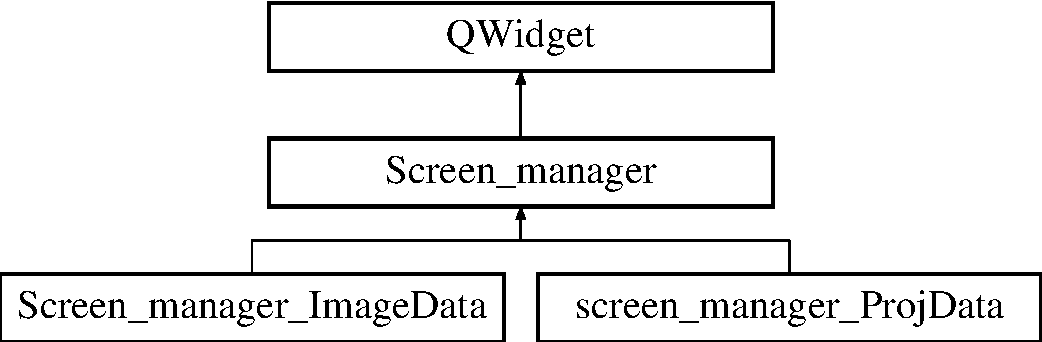
\includegraphics[height=3.000000cm]{classScreen__manager}
\end{center}
\end{figure}
\subsection*{Public Slots}
\begin{DoxyCompactItemize}
\item 
\mbox{\Hypertarget{classScreen__manager_a4a067888de043f5a73a56bc7f6eef4f6}\label{classScreen__manager_a4a067888de043f5a73a56bc7f6eef4f6}} 
virtual void {\bfseries save\+\_\+as\+\_\+array} (int this\+\_\+label)=0
\item 
\mbox{\Hypertarget{classScreen__manager_ac91e8b023e12dc15f8c6ab1951b4ce70}\label{classScreen__manager_ac91e8b023e12dc15f8c6ab1951b4ce70}} 
void {\bfseries remote\+\_\+scrbr\+\_\+value\+Changed} (const qint16 \&value)
\item 
\mbox{\Hypertarget{classScreen__manager_acfda6fcca2edd2d2a155b000256dad56}\label{classScreen__manager_acfda6fcca2edd2d2a155b000256dad56}} 
void {\bfseries remote\+\_\+relative\+\_\+scrbr\+\_\+value\+Changed} (qint32 value)
\item 
\mbox{\Hypertarget{classScreen__manager_a73a3bc131dbc70ce1eb689a890425227}\label{classScreen__manager_a73a3bc131dbc70ce1eb689a890425227}} 
virtual void {\bfseries on\+Cursor\+Changed} ()=0
\item 
\mbox{\Hypertarget{classScreen__manager_a91d823fd453b3d362ed06d5cf6cbdfb6}\label{classScreen__manager_a91d823fd453b3d362ed06d5cf6cbdfb6}} 
virtual void {\bfseries \+\_\+set\+Cursor} (const Q\+Point \&, Qwt\+Plot $\ast$)=0
\item 
\mbox{\Hypertarget{classScreen__manager_ae4cdc1ca921d3fb581c35d5df4c21d2b}\label{classScreen__manager_ae4cdc1ca921d3fb581c35d5df4c21d2b}} 
virtual void {\bfseries \+\_\+set\+Cursor} (const \mbox{\hyperlink{classViewer_1_1SimpleVector3D}{Viewer\+::\+Simple\+Vector3D}}$<$ int $>$ \&)=0
\item 
\mbox{\Hypertarget{classScreen__manager_a246b4fab17012a3b708613db86b7794f}\label{classScreen__manager_a246b4fab17012a3b708613db86b7794f}} 
virtual void {\bfseries update\+Cursor} (\mbox{\hyperlink{classdisplay__screen__container}{display\+\_\+screen\+\_\+container}} $\ast$d=0)=0
\item 
void \mbox{\hyperlink{classScreen__manager_afc206ddd1fee12c08d890d7a0c4c5fcb}{update\+All}} ()
\item 
void \mbox{\hyperlink{classScreen__manager_a0a17fba71b72fedefed5651b883ed371}{re\+Plot\+Plots}} ()
\item 
void \mbox{\hyperlink{classScreen__manager_a846061886a15cdc0de881976564b02f2}{refresh\+Plots}} ()
\end{DoxyCompactItemize}
\subsection*{Signals}
\begin{DoxyCompactItemize}
\item 
\mbox{\Hypertarget{classScreen__manager_acafc9314a77776acab7fafdca98c8aa6}\label{classScreen__manager_acafc9314a77776acab7fafdca98c8aa6}} 
void {\bfseries about\+To\+Close} ()
\item 
\mbox{\Hypertarget{classScreen__manager_a50d14535914f456dd55feeb2f54607f5}\label{classScreen__manager_a50d14535914f456dd55feeb2f54607f5}} 
void {\bfseries scrolled\+To} (qint16)
\item 
\mbox{\Hypertarget{classScreen__manager_a98ea0e9ea89f3e457b000b6cbabaa9d9}\label{classScreen__manager_a98ea0e9ea89f3e457b000b6cbabaa9d9}} 
void {\bfseries active\+Screen\+Updated} ()
\item 
\mbox{\Hypertarget{classScreen__manager_add6968bd7e6bedd1fe0d56e41e80a9d3}\label{classScreen__manager_add6968bd7e6bedd1fe0d56e41e80a9d3}} 
void \mbox{\hyperlink{classScreen__manager_add6968bd7e6bedd1fe0d56e41e80a9d3}{segment\+Changed\+To}} (Q\+String)
\begin{DoxyCompactList}\small\item\em segment\+Changed\+To This signal is emitted when the segment changes, in order to notify the rest of the group. \end{DoxyCompactList}\item 
\mbox{\Hypertarget{classScreen__manager_af30611f6463cf716bfe68d235a6884b2}\label{classScreen__manager_af30611f6463cf716bfe68d235a6884b2}} 
void {\bfseries set\+Color\+Map} (const qint16 \&)
\item 
\mbox{\Hypertarget{classScreen__manager_aa3779d6d7f3df9fcae204edb6bd03425}\label{classScreen__manager_aa3779d6d7f3df9fcae204edb6bd03425}} 
void {\bfseries updated\+Container} ()
\end{DoxyCompactItemize}
\subsection*{Public Member Functions}
\begin{DoxyCompactItemize}
\item 
\mbox{\Hypertarget{classScreen__manager_a6aa095225e7d6c68c49257298b048686}\label{classScreen__manager_a6aa095225e7d6c68c49257298b048686}} 
{\bfseries Screen\+\_\+manager} (\mbox{\hyperlink{classConfiguration}{Configuration}} $\ast$\+\_\+cur\+Config, Q\+Widget $\ast$parent)
\item 
\mbox{\Hypertarget{classScreen__manager_a35b2be90ae610b77457cd83793e6a9b7}\label{classScreen__manager_a35b2be90ae610b77457cd83793e6a9b7}} 
virtual bool {\bfseries load\+File} (const Q\+String file\+Name)=0
\item 
\mbox{\Hypertarget{classScreen__manager_a317d60e000518cd1af48d04dca139f43}\label{classScreen__manager_a317d60e000518cd1af48d04dca139f43}} 
\mbox{\hyperlink{classdisplay__screen__container}{display\+\_\+screen\+\_\+container}} $\ast$ \mbox{\hyperlink{classScreen__manager_a317d60e000518cd1af48d04dca139f43}{get\+Active\+Display\+Screen}} () const
\begin{DoxyCompactList}\small\item\em Returns the currently active container. \end{DoxyCompactList}\item 
\mbox{\Hypertarget{classScreen__manager_a26f4d66015d6788a69bf745309bfe93e}\label{classScreen__manager_a26f4d66015d6788a69bf745309bfe93e}} 
virtual Q\+Size {\bfseries set\+Orientation} (Orientation \+\_\+o=Next)=0
\item 
\mbox{\Hypertarget{classScreen__manager_a35fad2826491912a33af8f6b5192abc4}\label{classScreen__manager_a35fad2826491912a33af8f6b5192abc4}} 
Q\+String \mbox{\hyperlink{classScreen__manager_a35fad2826491912a33af8f6b5192abc4}{get\+Full\+File\+Path}} () const
\begin{DoxyCompactList}\small\item\em Get the my\+Full\+File\+Name. \end{DoxyCompactList}\item 
\mbox{\Hypertarget{classScreen__manager_acb7b0f59376ccbc2038b832bba22b577}\label{classScreen__manager_acb7b0f59376ccbc2038b832bba22b577}} 
void \mbox{\hyperlink{classScreen__manager_acb7b0f59376ccbc2038b832bba22b577}{set\+Full\+File\+Path}} (const Q\+String \&)
\begin{DoxyCompactList}\small\item\em Set the my\+Full\+File\+Name. \end{DoxyCompactList}\item 
\mbox{\Hypertarget{classScreen__manager_af2ea7252c092d06e846e6d50338db8ca}\label{classScreen__manager_af2ea7252c092d06e846e6d50338db8ca}} 
virtual Q\+String \mbox{\hyperlink{classScreen__manager_af2ea7252c092d06e846e6d50338db8ca}{get\+Data\+Type}} () const =0
\begin{DoxyCompactList}\small\item\em Returns image\+Data or proj\+Data. \end{DoxyCompactList}\item 
\mbox{\Hypertarget{classScreen__manager_ab773fd2975a54a2baaeb441b2644607d}\label{classScreen__manager_ab773fd2975a54a2baaeb441b2644607d}} 
Q\+String \mbox{\hyperlink{classScreen__manager_ab773fd2975a54a2baaeb441b2644607d}{get\+File\+Name}} () const
\begin{DoxyCompactList}\small\item\em Returns only the file\+Name. \end{DoxyCompactList}\item 
\mbox{\Hypertarget{classScreen__manager_a44503ee6f24482b8d01797503b0d88a8}\label{classScreen__manager_a44503ee6f24482b8d01797503b0d88a8}} 
qint16 \mbox{\hyperlink{classScreen__manager_a44503ee6f24482b8d01797503b0d88a8}{get\+Color\+Map\+Index}} () const
\begin{DoxyCompactList}\small\item\em Returnes the index of the current Color\+Map. \end{DoxyCompactList}\item 
\mbox{\Hypertarget{classScreen__manager_aec8c672544208e60368172e662de815e}\label{classScreen__manager_aec8c672544208e60368172e662de815e}} 
qint16 \mbox{\hyperlink{classScreen__manager_aec8c672544208e60368172e662de815e}{get\+Viewports\+Index}} () const
\item 
Simple\+Vector3D$<$ int $>$ $\ast$ \mbox{\hyperlink{classScreen__manager_a86a2c051954195c03f8718f4e371c221}{get\+Current\+Cursor}} () const
\item 
Cartesian\+Coordinate3D$<$ int $>$ $\ast$ \mbox{\hyperlink{classScreen__manager_a9cb3da1f84299ee2c32e4032e7e19ed1}{get\+Current\+Cursor}} () const
\item 
\mbox{\Hypertarget{classScreen__manager_a5437afdf92d233dfba71df3520861d2c}\label{classScreen__manager_a5437afdf92d233dfba71df3520861d2c}} 
virtual Cartesian\+Coordinate3D$<$ float $>$ $\ast$ \mbox{\hyperlink{classScreen__manager_a5437afdf92d233dfba71df3520861d2c}{get\+Current\+Cursor\+Inmm}} () const =0
\begin{DoxyCompactList}\small\item\em The current position of the current\+Cursor. \end{DoxyCompactList}\item 
\mbox{\Hypertarget{classScreen__manager_a6c41fbe3b06a11879010f8cce4488953}\label{classScreen__manager_a6c41fbe3b06a11879010f8cce4488953}} 
const Orientation $\ast$ \mbox{\hyperlink{classScreen__manager_a6c41fbe3b06a11879010f8cce4488953}{get\+Display\+Layout}} () const
\begin{DoxyCompactList}\small\item\em Returns the current display layout. \end{DoxyCompactList}\item 
\mbox{\Hypertarget{classScreen__manager_a15f0b7a953e3a15c46ccff31681f2c8d}\label{classScreen__manager_a15f0b7a953e3a15c46ccff31681f2c8d}} 
void \mbox{\hyperlink{classScreen__manager_a15f0b7a953e3a15c46ccff31681f2c8d}{set\+\_\+num\+\_\+viewports}} (qint16 num)
\item 
\mbox{\Hypertarget{classScreen__manager_ad86ad708eacc70d09ddfea3991c1436a}\label{classScreen__manager_ad86ad708eacc70d09ddfea3991c1436a}} 
void {\bfseries set\+Grouped} (bool)
\item 
\mbox{\Hypertarget{classScreen__manager_a1e9502d390457183eb1924753c3ffbaa}\label{classScreen__manager_a1e9502d390457183eb1924753c3ffbaa}} 
bool {\bfseries is\+Grouped} () const
\item 
\mbox{\Hypertarget{classScreen__manager_a491fb46b4eb96fb363848a1c506528bd}\label{classScreen__manager_a491fb46b4eb96fb363848a1c506528bd}} 
bool {\bfseries operator==} (const \mbox{\hyperlink{classScreen__manager}{Screen\+\_\+manager}} \&other) const
\item 
\mbox{\Hypertarget{classScreen__manager_a5f6269a00491d2dd64f4da8506f37d2f}\label{classScreen__manager_a5f6269a00491d2dd64f4da8506f37d2f}} 
bool {\bfseries operator!=} (const \mbox{\hyperlink{classScreen__manager}{Screen\+\_\+manager}} \&other) const
\item 
\mbox{\Hypertarget{classScreen__manager_a78723343009e85b288d800d9cc19bf80}\label{classScreen__manager_a78723343009e85b288d800d9cc19bf80}} 
\mbox{\hyperlink{classConfiguration}{Configuration}} $\ast$ {\bfseries get\+\_\+configuration} () const
\item 
\mbox{\Hypertarget{classScreen__manager_aad35e109d8d77378eb94605d10426a6f}\label{classScreen__manager_aad35e109d8d77378eb94605d10426a6f}} 
void {\bfseries block\+\_\+activity} (bool state)
\item 
\mbox{\Hypertarget{classScreen__manager_ac859de377f3ac1b7f18a9be9a21c193b}\label{classScreen__manager_ac859de377f3ac1b7f18a9be9a21c193b}} 
double \mbox{\hyperlink{classScreen__manager_ac859de377f3ac1b7f18a9be9a21c193b}{get\+\_\+min\+\_\+value\+\_\+all}} () const
\begin{DoxyCompactList}\small\item\em Return the minimum value of the entire dataset. \end{DoxyCompactList}\item 
\mbox{\Hypertarget{classScreen__manager_a39bc17ac270cdea092e20bed9d3a1e65}\label{classScreen__manager_a39bc17ac270cdea092e20bed9d3a1e65}} 
double \mbox{\hyperlink{classScreen__manager_a39bc17ac270cdea092e20bed9d3a1e65}{get\+\_\+max\+\_\+value\+\_\+all}} () const
\begin{DoxyCompactList}\small\item\em Return the maximum value of the entire dataset. \end{DoxyCompactList}\item 
\mbox{\Hypertarget{classScreen__manager_a7f44a2da2dbd75df0cc6dfc415ab764b}\label{classScreen__manager_a7f44a2da2dbd75df0cc6dfc415ab764b}} 
virtual int {\bfseries get\+Num\+Of\+Arrays} ()=0
\item 
\mbox{\Hypertarget{classScreen__manager_a918a7406704c29efb603df2dbd230277}\label{classScreen__manager_a918a7406704c29efb603df2dbd230277}} 
virtual Array$<$ 2, float $>$ {\bfseries get\+Array2D} (const int \&) const =0
\item 
\mbox{\Hypertarget{classScreen__manager_a48c42be07a7efc4b33e12a6364f4a8c3}\label{classScreen__manager_a48c42be07a7efc4b33e12a6364f4a8c3}} 
virtual void {\bfseries set\+Array2D} (const Array$<$ 2, float $>$ \&, const int \&)=0
\item 
\mbox{\Hypertarget{classScreen__manager_a4f66218cbf4962fa8582e8185f5b2b75}\label{classScreen__manager_a4f66218cbf4962fa8582e8185f5b2b75}} 
virtual void {\bfseries display} ()=0
\item 
\mbox{\Hypertarget{classScreen__manager_ad1cd939deb35910262eaa503018ea1b6}\label{classScreen__manager_ad1cd939deb35910262eaa503018ea1b6}} 
void {\bfseries set\+\_\+multiple\+\_\+selections\+\_\+allowed} (bool state)
\item 
\mbox{\Hypertarget{classScreen__manager_ac67d1eb96f39a7f38fff5554e23185a3}\label{classScreen__manager_ac67d1eb96f39a7f38fff5554e23185a3}} 
virtual void \mbox{\hyperlink{classScreen__manager_ac67d1eb96f39a7f38fff5554e23185a3}{show\+Cursor}} (const bool \&state)=0
\begin{DoxyCompactList}\small\item\em Display a blue cross on the location of current\+Cursor. \end{DoxyCompactList}\item 
\mbox{\Hypertarget{classScreen__manager_afb1943d5f00971d44c607a35d2f14400}\label{classScreen__manager_afb1943d5f00971d44c607a35d2f14400}} 
bool {\bfseries get\+Cursor\+Status} () const
\item 
\mbox{\Hypertarget{classScreen__manager_a2f34df85df98b630cc76c44f95191b0c}\label{classScreen__manager_a2f34df85df98b630cc76c44f95191b0c}} 
double {\bfseries get\+Current\+Value} ()
\item 
\mbox{\Hypertarget{classScreen__manager_ae6a57554e55917af3be9d57b903e5705}\label{classScreen__manager_ae6a57554e55917af3be9d57b903e5705}} 
virtual const Index\+Range$<$ 3 $>$ {\bfseries get\+Ranges3D} ()=0
\item 
\mbox{\Hypertarget{classScreen__manager_a34e5e5c557ba96660e7fefd09647952e}\label{classScreen__manager_a34e5e5c557ba96660e7fefd09647952e}} 
virtual void \mbox{\hyperlink{classScreen__manager_a34e5e5c557ba96660e7fefd09647952e}{write\+To\+Disk}} (const Q\+String \&)=0
\begin{DoxyCompactList}\small\item\em Write data to disk using S\+T\+IR functions. \end{DoxyCompactList}\item 
\mbox{\Hypertarget{classScreen__manager_ae1be547f78a67154e879922d953fb500}\label{classScreen__manager_ae1be547f78a67154e879922d953fb500}} 
virtual void \mbox{\hyperlink{classScreen__manager_ae1be547f78a67154e879922d953fb500}{apply\+Viz\+Values\+To\+All\+Containers}} (const double \&\+\_\+min, const double \&\+\_\+max)=0
\begin{DoxyCompactList}\small\item\em Set the viz\+\_\+min and viz\+\_\+max values at all containers. \end{DoxyCompactList}\item 
\mbox{\Hypertarget{classScreen__manager_ac89b57e0751e9a9c65e620b0f0ea04ab}\label{classScreen__manager_ac89b57e0751e9a9c65e620b0f0ea04ab}} 
virtual void {\bfseries apply\+Function\+To\+All\+Containers} (\mbox{\hyperlink{classWorker}{Worker}} $\ast$\+\_\+w)=0
\item 
\mbox{\Hypertarget{classScreen__manager_a8f1b65a9a4683531a81006ff90f0784a}\label{classScreen__manager_a8f1b65a9a4683531a81006ff90f0784a}} 
virtual void {\bfseries remove\+Function\+To\+All\+Containers} ()=0
\item 
\mbox{\Hypertarget{classScreen__manager_a561aa42a8717049bd6f481d0e28e1a05}\label{classScreen__manager_a561aa42a8717049bd6f481d0e28e1a05}} 
virtual Voxels\+On\+Cartesian\+Grid$<$ float $>$ $\ast$ {\bfseries get\+Data\+\_\+ptr} ()=0
\end{DoxyCompactItemize}
\subsection*{Public Attributes}
\begin{DoxyCompactItemize}
\item 
\mbox{\Hypertarget{classScreen__manager_ad20150bef59ac873d47c7dccb5062258}\label{classScreen__manager_ad20150bef59ac873d47c7dccb5062258}} 
Q\+Vector$<$ std\+::shared\+\_\+ptr$<$ \mbox{\hyperlink{classdisplay__screen__container}{display\+\_\+screen\+\_\+container}} $>$ $>$ {\bfseries my\+\_\+containers}
\end{DoxyCompactItemize}
\subsection*{Protected Slots}
\begin{DoxyCompactItemize}
\item 
\mbox{\Hypertarget{classScreen__manager_a9f814711fe49f63a404758ffb39f63cc}\label{classScreen__manager_a9f814711fe49f63a404758ffb39f63cc}} 
void {\bfseries set\+Active\+Screen\+Container} (const qint32 \&)
\end{DoxyCompactItemize}
\subsection*{Protected Member Functions}
\begin{DoxyCompactItemize}
\item 
\mbox{\Hypertarget{classScreen__manager_a8285b74dd2913a8368aebb8c4aeccee1}\label{classScreen__manager_a8285b74dd2913a8368aebb8c4aeccee1}} 
virtual void {\bfseries set\+\_\+up\+\_\+plot\+\_\+area} ()
\item 
\mbox{\Hypertarget{classScreen__manager_a5f8b8efd36388e8d60a1c5d78d458b2d}\label{classScreen__manager_a5f8b8efd36388e8d60a1c5d78d458b2d}} 
virtual double {\bfseries get\+Value\+At} (const \mbox{\hyperlink{classViewer_1_1SimpleVector3D}{Simple\+Vector3D}}$<$ int $>$ \+\_\+c)=0
\item 
\mbox{\Hypertarget{classScreen__manager_a1e77461fc2c621a338131d25efa28e7a}\label{classScreen__manager_a1e77461fc2c621a338131d25efa28e7a}} 
void {\bfseries close\+Event} (Q\+Close\+Event $\ast$event) override
\item 
\mbox{\Hypertarget{classScreen__manager_ae999da71a66db6ce0ce62216fe20863a}\label{classScreen__manager_ae999da71a66db6ce0ce62216fe20863a}} 
void \mbox{\hyperlink{classScreen__manager_ae999da71a66db6ce0ce62216fe20863a}{set\+Up\+Containers}} (int \+\_\+num=3)
\begin{DoxyCompactList}\small\item\em Initializes the \mbox{\hyperlink{classdisplay__screen__container}{display\+\_\+screen\+\_\+container}}. /todo The default 3 must change to zero. \end{DoxyCompactList}\item 
void \mbox{\hyperlink{classScreen__manager_a5896c354d45b0b4142a76b26f7081787}{clear\+Containers}} ()
\end{DoxyCompactItemize}
\subsection*{Protected Attributes}
\begin{DoxyCompactItemize}
\item 
\mbox{\Hypertarget{classScreen__manager_a08d9ac0f5ff1946873ceafa1c91fd5bf}\label{classScreen__manager_a08d9ac0f5ff1946873ceafa1c91fd5bf}} 
Ui\+::\+Screen\+\_\+manager $\ast$ {\bfseries ui}
\item 
\mbox{\Hypertarget{classScreen__manager_aca1b3a8cf4a318e3c6a90c8886389cc6}\label{classScreen__manager_aca1b3a8cf4a318e3c6a90c8886389cc6}} 
Q\+String {\bfseries my\+Full\+File\+Name}
\item 
\mbox{\Hypertarget{classScreen__manager_a0677c1654b984e635d160189de4c77ad}\label{classScreen__manager_a0677c1654b984e635d160189de4c77ad}} 
Orientation \mbox{\hyperlink{classScreen__manager_a0677c1654b984e635d160189de4c77ad}{view\+Order}}
\begin{DoxyCompactList}\small\item\em The current Orientation on display. Since Orientation\+::\+All. \end{DoxyCompactList}\item 
\mbox{\Hypertarget{classScreen__manager_add6a20bb797b0a544aed8b84371a4f24}\label{classScreen__manager_add6a20bb797b0a544aed8b84371a4f24}} 
\mbox{\hyperlink{classConfiguration}{Configuration}} $\ast$ \mbox{\hyperlink{classScreen__manager_add6a20bb797b0a544aed8b84371a4f24}{cur\+Config}}
\begin{DoxyCompactList}\small\item\em \mbox{\hyperlink{classConfiguration}{Configuration}} doesn\textquotesingle{}t do a lot, yet. \end{DoxyCompactList}\item 
\mbox{\Hypertarget{classScreen__manager_a8b9367dee1bb7f7b76b7c8b7fd219f6c}\label{classScreen__manager_a8b9367dee1bb7f7b76b7c8b7fd219f6c}} 
\mbox{\hyperlink{classViewer_1_1SimpleVector3D}{Simple\+Vector3D}}$<$ int $>$ $\ast$ \mbox{\hyperlink{classScreen__manager_a8b9367dee1bb7f7b76b7c8b7fd219f6c}{current\+Cursor}}
\begin{DoxyCompactList}\small\item\em The current position it is shared as a pointer in the \mbox{\hyperlink{classdisplay__screen__container}{display\+\_\+screen\+\_\+container}}. \end{DoxyCompactList}\item 
\mbox{\Hypertarget{classScreen__manager_ac1552176fcb2eec1f3f71139933b38b6}\label{classScreen__manager_ac1552176fcb2eec1f3f71139933b38b6}} 
\mbox{\hyperlink{classdisplay__screen__container}{display\+\_\+screen\+\_\+container}} $\ast$ \mbox{\hyperlink{classScreen__manager_ac1552176fcb2eec1f3f71139933b38b6}{active\+Screen\+Contrainer}}
\begin{DoxyCompactList}\small\item\em This is the active \mbox{\hyperlink{classdisplay__screen__container}{display\+\_\+screen\+\_\+container}}. \end{DoxyCompactList}\item 
\mbox{\Hypertarget{classScreen__manager_a9aa51b589844972991a3b234ccf17aa4}\label{classScreen__manager_a9aa51b589844972991a3b234ccf17aa4}} 
bool \mbox{\hyperlink{classScreen__manager_a9aa51b589844972991a3b234ccf17aa4}{cursor\+Status}}
\begin{DoxyCompactList}\small\item\em It indicates wether the blue cross is printed on the displays. \end{DoxyCompactList}\item 
\mbox{\Hypertarget{classScreen__manager_ad88254b68805043118c3fb66009bad6b}\label{classScreen__manager_ad88254b68805043118c3fb66009bad6b}} 
bool \mbox{\hyperlink{classScreen__manager_ad88254b68805043118c3fb66009bad6b}{containers\+Ready}}
\begin{DoxyCompactList}\small\item\em True if the containers have been initialized properly. \end{DoxyCompactList}\item 
\mbox{\Hypertarget{classScreen__manager_a65684948bf1429005ea9f1a507d50e49}\label{classScreen__manager_a65684948bf1429005ea9f1a507d50e49}} 
double \mbox{\hyperlink{classScreen__manager_a65684948bf1429005ea9f1a507d50e49}{min\+Value\+All}}
\begin{DoxyCompactList}\small\item\em The minimum value of the entire dataset. \end{DoxyCompactList}\item 
\mbox{\Hypertarget{classScreen__manager_a8d46413c932ecafedb06fd9b0ee1d6b1}\label{classScreen__manager_a8d46413c932ecafedb06fd9b0ee1d6b1}} 
double \mbox{\hyperlink{classScreen__manager_a8d46413c932ecafedb06fd9b0ee1d6b1}{max\+Value\+All}}
\begin{DoxyCompactList}\small\item\em The maximum value of the entire dataset. \end{DoxyCompactList}\end{DoxyCompactItemize}


\subsection{Member Function Documentation}
\mbox{\Hypertarget{classScreen__manager_a5896c354d45b0b4142a76b26f7081787}\label{classScreen__manager_a5896c354d45b0b4142a76b26f7081787}} 
\index{Screen\+\_\+manager@{Screen\+\_\+manager}!clear\+Containers@{clear\+Containers}}
\index{clear\+Containers@{clear\+Containers}!Screen\+\_\+manager@{Screen\+\_\+manager}}
\subsubsection{\texorpdfstring{clear\+Containers()}{clearContainers()}}
{\footnotesize\ttfamily void Screen\+\_\+manager\+::clear\+Containers (\begin{DoxyParamCaption}{ }\end{DoxyParamCaption})\hspace{0.3cm}{\ttfamily [protected]}}

Erase the \mbox{\hyperlink{classdisplay__screen__container}{display\+\_\+screen\+\_\+container}}. Since I keep all views in memory this might be . \mbox{\Hypertarget{classScreen__manager_a86a2c051954195c03f8718f4e371c221}\label{classScreen__manager_a86a2c051954195c03f8718f4e371c221}} 
\index{Screen\+\_\+manager@{Screen\+\_\+manager}!get\+Current\+Cursor@{get\+Current\+Cursor}}
\index{get\+Current\+Cursor@{get\+Current\+Cursor}!Screen\+\_\+manager@{Screen\+\_\+manager}}
\subsubsection{\texorpdfstring{get\+Current\+Cursor()}{getCurrentCursor()}\hspace{0.1cm}{\footnotesize\ttfamily [1/2]}}
{\footnotesize\ttfamily Simple\+Vector3D$<$ int $>$ $\ast$ Screen\+\_\+manager\+::get\+Current\+Cursor (\begin{DoxyParamCaption}{ }\end{DoxyParamCaption}) const\hspace{0.3cm}{\ttfamily [inline]}}

The current position of the current\+Cursor, overloaded function returning \mbox{\hyperlink{classViewer_1_1SimpleVector3D}{Simple\+Vector3\+D$<$int$>$}} \mbox{\Hypertarget{classScreen__manager_a9cb3da1f84299ee2c32e4032e7e19ed1}\label{classScreen__manager_a9cb3da1f84299ee2c32e4032e7e19ed1}} 
\index{Screen\+\_\+manager@{Screen\+\_\+manager}!get\+Current\+Cursor@{get\+Current\+Cursor}}
\index{get\+Current\+Cursor@{get\+Current\+Cursor}!Screen\+\_\+manager@{Screen\+\_\+manager}}
\subsubsection{\texorpdfstring{get\+Current\+Cursor()}{getCurrentCursor()}\hspace{0.1cm}{\footnotesize\ttfamily [2/2]}}
{\footnotesize\ttfamily Cartesian\+Coordinate3D$<$int$>$$\ast$ Screen\+\_\+manager\+::get\+Current\+Cursor (\begin{DoxyParamCaption}{ }\end{DoxyParamCaption}) const\hspace{0.3cm}{\ttfamily [inline]}}

The current position of the current\+Cursor, overloaded function returning Cartesian\+Coordinate3\+D$<$int$>$ \mbox{\Hypertarget{classScreen__manager_a846061886a15cdc0de881976564b02f2}\label{classScreen__manager_a846061886a15cdc0de881976564b02f2}} 
\index{Screen\+\_\+manager@{Screen\+\_\+manager}!refresh\+Plots@{refresh\+Plots}}
\index{refresh\+Plots@{refresh\+Plots}!Screen\+\_\+manager@{Screen\+\_\+manager}}
\subsubsection{\texorpdfstring{refresh\+Plots}{refreshPlots}}
{\footnotesize\ttfamily void Screen\+\_\+manager\+::refresh\+Plots (\begin{DoxyParamCaption}{ }\end{DoxyParamCaption})\hspace{0.3cm}{\ttfamily [slot]}}

This is a ligher version of \mbox{\hyperlink{classScreen__manager_a0a17fba71b72fedefed5651b883ed371}{re\+Plot\+Plots()}}, where the plots are replotted without rereading the data. \mbox{\Hypertarget{classScreen__manager_a0a17fba71b72fedefed5651b883ed371}\label{classScreen__manager_a0a17fba71b72fedefed5651b883ed371}} 
\index{Screen\+\_\+manager@{Screen\+\_\+manager}!re\+Plot\+Plots@{re\+Plot\+Plots}}
\index{re\+Plot\+Plots@{re\+Plot\+Plots}!Screen\+\_\+manager@{Screen\+\_\+manager}}
\subsubsection{\texorpdfstring{re\+Plot\+Plots}{rePlotPlots}}
{\footnotesize\ttfamily void Screen\+\_\+manager\+::re\+Plot\+Plots (\begin{DoxyParamCaption}{ }\end{DoxyParamCaption})\hspace{0.3cm}{\ttfamily [slot]}}

Calls display\+\_\+screen\+\_\+container\+::update\+Plot\+Area for every my\+\_\+container. Effectively the data will be reread. \mbox{\Hypertarget{classScreen__manager_afc206ddd1fee12c08d890d7a0c4c5fcb}\label{classScreen__manager_afc206ddd1fee12c08d890d7a0c4c5fcb}} 
\index{Screen\+\_\+manager@{Screen\+\_\+manager}!update\+All@{update\+All}}
\index{update\+All@{update\+All}!Screen\+\_\+manager@{Screen\+\_\+manager}}
\subsubsection{\texorpdfstring{update\+All}{updateAll}}
{\footnotesize\ttfamily void Screen\+\_\+manager\+::update\+All (\begin{DoxyParamCaption}{ }\end{DoxyParamCaption})\hspace{0.3cm}{\ttfamily [slot]}}

It will recalculate the minimum and maximum values and replot the screens. 

The documentation for this class was generated from the following files\+:\begin{DoxyCompactItemize}
\item 
src/display\+\_\+buildblock/screen\+\_\+manager.\+h\item 
src/display\+\_\+buildblock/screen\+\_\+manager.\+cpp\item 
src/display\+\_\+buildblock/screen\+\_\+manager.\+inl\end{DoxyCompactItemize}

\hypertarget{classScreen__manager__ImageData}{}\section{Screen\+\_\+manager\+\_\+\+Image\+Data Class Reference}
\label{classScreen__manager__ImageData}\index{Screen\+\_\+manager\+\_\+\+Image\+Data@{Screen\+\_\+manager\+\_\+\+Image\+Data}}
Inheritance diagram for Screen\+\_\+manager\+\_\+\+Image\+Data\+:\begin{figure}[H]
\begin{center}
\leavevmode
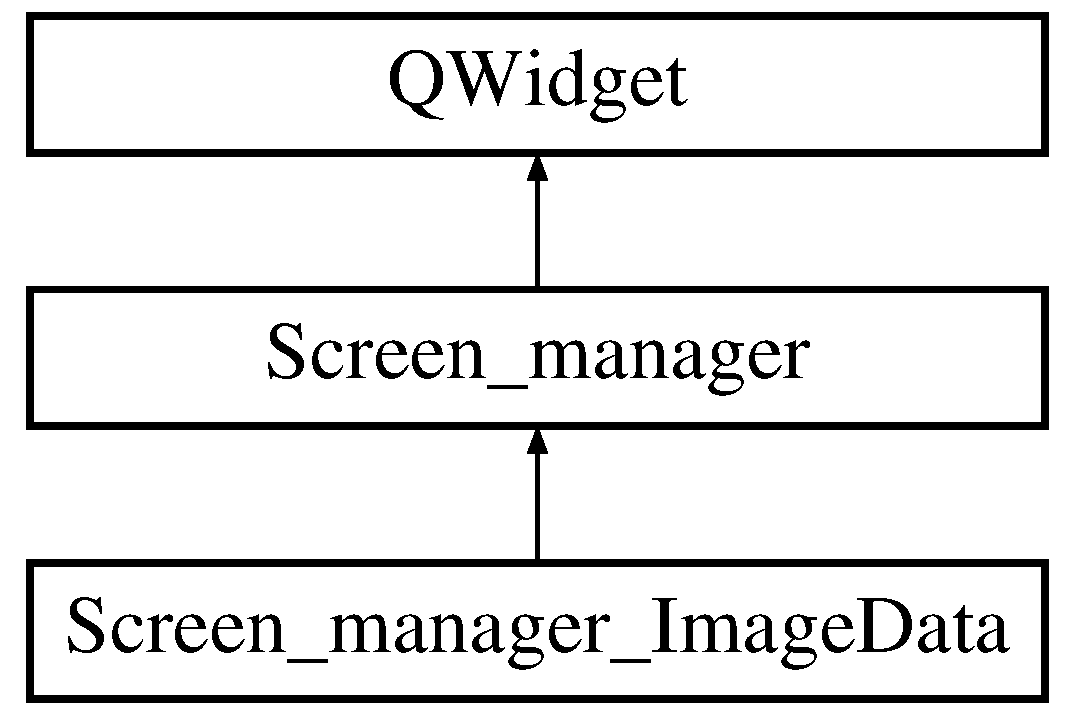
\includegraphics[height=3.000000cm]{classScreen__manager__ImageData}
\end{center}
\end{figure}
\subsection*{Public Slots}
\begin{DoxyCompactItemize}
\item 
\mbox{\Hypertarget{classScreen__manager__ImageData_aa862cab6cf8d631117550f5e1db6da67}\label{classScreen__manager__ImageData_aa862cab6cf8d631117550f5e1db6da67}} 
void {\bfseries on\+Cursor\+Changed} ()
\item 
\mbox{\Hypertarget{classScreen__manager__ImageData_ae20130e2cad07bc6b88917cea5408691}\label{classScreen__manager__ImageData_ae20130e2cad07bc6b88917cea5408691}} 
virtual void {\bfseries \+\_\+set\+Cursor} (const Q\+Point \&, Qwt\+Plot $\ast$)
\item 
\mbox{\Hypertarget{classScreen__manager__ImageData_aeeada64fe7a1c797dc601dfc221b6713}\label{classScreen__manager__ImageData_aeeada64fe7a1c797dc601dfc221b6713}} 
virtual void {\bfseries \+\_\+set\+Cursor} (const \mbox{\hyperlink{classViewer_1_1SimpleVector3D}{Viewer\+::\+Simple\+Vector3D}}$<$ int $>$ \&)
\item 
\mbox{\Hypertarget{classScreen__manager__ImageData_a0da8dec9cda46dcaa0011d1b666490e9}\label{classScreen__manager__ImageData_a0da8dec9cda46dcaa0011d1b666490e9}} 
virtual void {\bfseries update\+Cursor} (\mbox{\hyperlink{classdisplay__screen__container}{display\+\_\+screen\+\_\+container}} $\ast$d=0)
\item 
\mbox{\Hypertarget{classScreen__manager_ac91e8b023e12dc15f8c6ab1951b4ce70}\label{classScreen__manager_ac91e8b023e12dc15f8c6ab1951b4ce70}} 
void {\bfseries remote\+\_\+scrbr\+\_\+value\+Changed} (const qint16 \&value)
\item 
\mbox{\Hypertarget{classScreen__manager_acfda6fcca2edd2d2a155b000256dad56}\label{classScreen__manager_acfda6fcca2edd2d2a155b000256dad56}} 
void {\bfseries remote\+\_\+relative\+\_\+scrbr\+\_\+value\+Changed} (qint32 value)
\item 
void \mbox{\hyperlink{classScreen__manager_afc206ddd1fee12c08d890d7a0c4c5fcb}{update\+All}} ()
\item 
void \mbox{\hyperlink{classScreen__manager_a0a17fba71b72fedefed5651b883ed371}{re\+Plot\+Plots}} ()
\item 
void \mbox{\hyperlink{classScreen__manager_a846061886a15cdc0de881976564b02f2}{refresh\+Plots}} ()
\end{DoxyCompactItemize}
\subsection*{Signals}
\begin{DoxyCompactItemize}
\item 
\mbox{\Hypertarget{classScreen__manager_acafc9314a77776acab7fafdca98c8aa6}\label{classScreen__manager_acafc9314a77776acab7fafdca98c8aa6}} 
void {\bfseries about\+To\+Close} ()
\item 
\mbox{\Hypertarget{classScreen__manager_a50d14535914f456dd55feeb2f54607f5}\label{classScreen__manager_a50d14535914f456dd55feeb2f54607f5}} 
void {\bfseries scrolled\+To} (qint16)
\item 
\mbox{\Hypertarget{classScreen__manager_a98ea0e9ea89f3e457b000b6cbabaa9d9}\label{classScreen__manager_a98ea0e9ea89f3e457b000b6cbabaa9d9}} 
void {\bfseries active\+Screen\+Updated} ()
\item 
\mbox{\Hypertarget{classScreen__manager_add6968bd7e6bedd1fe0d56e41e80a9d3}\label{classScreen__manager_add6968bd7e6bedd1fe0d56e41e80a9d3}} 
void \mbox{\hyperlink{classScreen__manager_add6968bd7e6bedd1fe0d56e41e80a9d3}{segment\+Changed\+To}} (Q\+String)
\begin{DoxyCompactList}\small\item\em segment\+Changed\+To This signal is emitted when the segment changes, in order to notify the rest of the group. \end{DoxyCompactList}\item 
\mbox{\Hypertarget{classScreen__manager_af30611f6463cf716bfe68d235a6884b2}\label{classScreen__manager_af30611f6463cf716bfe68d235a6884b2}} 
void {\bfseries set\+Color\+Map} (const qint16 \&)
\item 
\mbox{\Hypertarget{classScreen__manager_aa3779d6d7f3df9fcae204edb6bd03425}\label{classScreen__manager_aa3779d6d7f3df9fcae204edb6bd03425}} 
void {\bfseries updated\+Container} ()
\end{DoxyCompactItemize}
\subsection*{Public Member Functions}
\begin{DoxyCompactItemize}
\item 
\mbox{\Hypertarget{classScreen__manager__ImageData_ae2c06f1e08b0dce97fa29564c09b363a}\label{classScreen__manager__ImageData_ae2c06f1e08b0dce97fa29564c09b363a}} 
{\bfseries Screen\+\_\+manager\+\_\+\+Image\+Data} (\mbox{\hyperlink{classConfiguration}{Configuration}} $\ast$\mbox{\hyperlink{classScreen__manager_add6a20bb797b0a544aed8b84371a4f24}{cur\+Config}}, Q\+Widget $\ast$parent)
\item 
\mbox{\Hypertarget{classScreen__manager__ImageData_aaa3133f02c9f659784c543d9123dad41}\label{classScreen__manager__ImageData_aaa3133f02c9f659784c543d9123dad41}} 
{\bfseries Screen\+\_\+manager\+\_\+\+Image\+Data} (Voxels\+On\+Cartesian\+Grid$<$ float $>$ $\ast$image, \mbox{\hyperlink{classConfiguration}{Configuration}} $\ast$\mbox{\hyperlink{classScreen__manager_add6a20bb797b0a544aed8b84371a4f24}{cur\+Config}}, Q\+Widget $\ast$parent)
\item 
\mbox{\Hypertarget{classScreen__manager__ImageData_a6892a6ecf23c6c989138a3dd1c6bbb02}\label{classScreen__manager__ImageData_a6892a6ecf23c6c989138a3dd1c6bbb02}} 
virtual bool {\bfseries load\+File} (const Q\+String file\+Name)
\item 
\mbox{\Hypertarget{classScreen__manager__ImageData_aea1b49dd7e2ee80c81ec270b97788764}\label{classScreen__manager__ImageData_aea1b49dd7e2ee80c81ec270b97788764}} 
bool {\bfseries set\+State} (qint16 new\+View\+Order, qint16 new\+\_\+current\+\_\+id, qint16 new\+\_\+num\+\_\+viewports)
\item 
\mbox{\Hypertarget{classScreen__manager__ImageData_ae977853c806bf1b7eee47ee4eefb74e4}\label{classScreen__manager__ImageData_ae977853c806bf1b7eee47ee4eefb74e4}} 
virtual Q\+Size {\bfseries set\+Orientation} (Orientation \+\_\+o=Next)
\item 
\mbox{\Hypertarget{classScreen__manager__ImageData_a16f2f25a0bdc587ace3cbddeb2bdc925}\label{classScreen__manager__ImageData_a16f2f25a0bdc587ace3cbddeb2bdc925}} 
virtual Q\+String \mbox{\hyperlink{classScreen__manager__ImageData_a16f2f25a0bdc587ace3cbddeb2bdc925}{get\+Data\+Type}} () const
\begin{DoxyCompactList}\small\item\em Returns image\+Data or proj\+Data. \end{DoxyCompactList}\item 
\mbox{\Hypertarget{classScreen__manager__ImageData_a70e5f3c33181d6e4747507b0e64dbd8c}\label{classScreen__manager__ImageData_a70e5f3c33181d6e4747507b0e64dbd8c}} 
Voxels\+On\+Cartesian\+Grid$<$ float $>$ {\bfseries get\+\_\+subset} (const Index\+Range$<$ 3 $>$ \&new\+\_\+range, const int \&\+\_\+minZ, const int \&\+\_\+maxZ)
\item 
\mbox{\Hypertarget{classScreen__manager__ImageData_af4f49a263400404afc11e60f2cec6dc3}\label{classScreen__manager__ImageData_af4f49a263400404afc11e60f2cec6dc3}} 
void {\bfseries get\+\_\+subset} (Voxels\+On\+Cartesian\+Grid$<$ float $>$ \&\+\_\+tmp, const Index\+Range$<$ 3 $>$ \&new\+\_\+range, const int \&\+\_\+minZ, const int \&\+\_\+maxZ)
\item 
\mbox{\Hypertarget{classScreen__manager__ImageData_a65b825f8b263a44fa7051718c8d20393}\label{classScreen__manager__ImageData_a65b825f8b263a44fa7051718c8d20393}} 
Index\+Range$<$ 3 $>$ {\bfseries get\+\_\+\+Index\+Range} () const
\item 
\mbox{\Hypertarget{classScreen__manager__ImageData_a104cb0590753cd20fb2b2c027a451d68}\label{classScreen__manager__ImageData_a104cb0590753cd20fb2b2c027a451d68}} 
virtual Voxels\+On\+Cartesian\+Grid$<$ float $>$ $\ast$ {\bfseries get\+Data\+\_\+ptr} ()
\item 
\mbox{\Hypertarget{classScreen__manager__ImageData_ae65fbfbe7d3a9aa39b15e5438b18e47f}\label{classScreen__manager__ImageData_ae65fbfbe7d3a9aa39b15e5438b18e47f}} 
virtual int {\bfseries get\+Num\+Of\+Arrays} ()
\item 
\mbox{\Hypertarget{classScreen__manager__ImageData_a8c814021e716030a78e68991132095cd}\label{classScreen__manager__ImageData_a8c814021e716030a78e68991132095cd}} 
virtual Array$<$ 2, float $>$ {\bfseries get\+Array2D} (const int \&) const
\item 
\mbox{\Hypertarget{classScreen__manager__ImageData_a27813e2dfc1bf53b8f82bca9451b8686}\label{classScreen__manager__ImageData_a27813e2dfc1bf53b8f82bca9451b8686}} 
virtual void {\bfseries set\+Array2D} (const Array$<$ 2, float $>$ \&, const int \&)
\item 
\mbox{\Hypertarget{classScreen__manager__ImageData_a1a50b73c42c5991bd0491c16dfebfa74}\label{classScreen__manager__ImageData_a1a50b73c42c5991bd0491c16dfebfa74}} 
virtual void {\bfseries display} ()
\item 
\mbox{\Hypertarget{classScreen__manager__ImageData_a06b0b13e9e13016877ce148a6fbea5d9}\label{classScreen__manager__ImageData_a06b0b13e9e13016877ce148a6fbea5d9}} 
void {\bfseries split} (const int \&split\+\_\+slice, Q\+Vector$<$ \mbox{\hyperlink{classScreen__manager__ImageData}{Screen\+\_\+manager\+\_\+\+Image\+Data}} $\ast$$>$ \&ret\+\_\+list)
\item 
\mbox{\Hypertarget{classScreen__manager__ImageData_a6cd2d1f4164dae4ebdbe16eeb055f2f9}\label{classScreen__manager__ImageData_a6cd2d1f4164dae4ebdbe16eeb055f2f9}} 
virtual void \mbox{\hyperlink{classScreen__manager__ImageData_a6cd2d1f4164dae4ebdbe16eeb055f2f9}{show\+Cursor}} (const bool \&state=false)
\begin{DoxyCompactList}\small\item\em Display a blue cross on the location of current\+Cursor. \end{DoxyCompactList}\item 
\mbox{\Hypertarget{classScreen__manager__ImageData_a7d9def64f1dbbf5aaa88d18bf13734d3}\label{classScreen__manager__ImageData_a7d9def64f1dbbf5aaa88d18bf13734d3}} 
virtual const Index\+Range$<$ 3 $>$ {\bfseries get\+Ranges3D} ()
\item 
\mbox{\Hypertarget{classScreen__manager__ImageData_a10d265f8f1f7e027fe2dcd99cf549ec8}\label{classScreen__manager__ImageData_a10d265f8f1f7e027fe2dcd99cf549ec8}} 
virtual void \mbox{\hyperlink{classScreen__manager__ImageData_a10d265f8f1f7e027fe2dcd99cf549ec8}{write\+To\+Disk}} (const Q\+String \&\+\_\+p)
\begin{DoxyCompactList}\small\item\em Write image to disk using S\+T\+IR functions. \end{DoxyCompactList}\item 
\mbox{\Hypertarget{classScreen__manager__ImageData_ad83bf93759160752b782a9e70cddcc77}\label{classScreen__manager__ImageData_ad83bf93759160752b782a9e70cddcc77}} 
virtual void \mbox{\hyperlink{classScreen__manager__ImageData_ad83bf93759160752b782a9e70cddcc77}{apply\+Viz\+Values\+To\+All\+Containers}} (const double \&\+\_\+min, const double \&\+\_\+max)
\begin{DoxyCompactList}\small\item\em Set the viz\+\_\+min and viz\+\_\+max values at all containers. \end{DoxyCompactList}\item 
\mbox{\Hypertarget{classScreen__manager__ImageData_a8e281d0c897f560882d7ab7d0e9c097d}\label{classScreen__manager__ImageData_a8e281d0c897f560882d7ab7d0e9c097d}} 
virtual void {\bfseries apply\+Function\+To\+All\+Containers} (\mbox{\hyperlink{classWorker}{Worker}} $\ast$\+\_\+w)
\item 
\mbox{\Hypertarget{classScreen__manager__ImageData_a3f6a84be6747401ec25a6236f441003a}\label{classScreen__manager__ImageData_a3f6a84be6747401ec25a6236f441003a}} 
virtual void {\bfseries remove\+Function\+To\+All\+Containers} ()
\item 
\mbox{\Hypertarget{classScreen__manager__ImageData_a732195e4fae93f0f725df94c7a0b3ef7}\label{classScreen__manager__ImageData_a732195e4fae93f0f725df94c7a0b3ef7}} 
virtual Cartesian\+Coordinate3D$<$ float $>$ $\ast$ \mbox{\hyperlink{classScreen__manager__ImageData_a732195e4fae93f0f725df94c7a0b3ef7}{get\+Current\+Cursor\+Inmm}} () const =0
\begin{DoxyCompactList}\small\item\em The current position of the current\+Cursor. \end{DoxyCompactList}\item 
\mbox{\Hypertarget{classScreen__manager_a317d60e000518cd1af48d04dca139f43}\label{classScreen__manager_a317d60e000518cd1af48d04dca139f43}} 
\mbox{\hyperlink{classdisplay__screen__container}{display\+\_\+screen\+\_\+container}} $\ast$ \mbox{\hyperlink{classScreen__manager_a317d60e000518cd1af48d04dca139f43}{get\+Active\+Display\+Screen}} () const
\begin{DoxyCompactList}\small\item\em Returns the currently active container. \end{DoxyCompactList}\item 
\mbox{\Hypertarget{classScreen__manager_a35fad2826491912a33af8f6b5192abc4}\label{classScreen__manager_a35fad2826491912a33af8f6b5192abc4}} 
Q\+String \mbox{\hyperlink{classScreen__manager_a35fad2826491912a33af8f6b5192abc4}{get\+Full\+File\+Path}} () const
\begin{DoxyCompactList}\small\item\em Get the my\+Full\+File\+Name. \end{DoxyCompactList}\item 
\mbox{\Hypertarget{classScreen__manager_acb7b0f59376ccbc2038b832bba22b577}\label{classScreen__manager_acb7b0f59376ccbc2038b832bba22b577}} 
void \mbox{\hyperlink{classScreen__manager_acb7b0f59376ccbc2038b832bba22b577}{set\+Full\+File\+Path}} (const Q\+String \&)
\begin{DoxyCompactList}\small\item\em Set the my\+Full\+File\+Name. \end{DoxyCompactList}\item 
\mbox{\Hypertarget{classScreen__manager_ab773fd2975a54a2baaeb441b2644607d}\label{classScreen__manager_ab773fd2975a54a2baaeb441b2644607d}} 
Q\+String \mbox{\hyperlink{classScreen__manager_ab773fd2975a54a2baaeb441b2644607d}{get\+File\+Name}} () const
\begin{DoxyCompactList}\small\item\em Returns only the file\+Name. \end{DoxyCompactList}\item 
\mbox{\Hypertarget{classScreen__manager_a44503ee6f24482b8d01797503b0d88a8}\label{classScreen__manager_a44503ee6f24482b8d01797503b0d88a8}} 
qint16 \mbox{\hyperlink{classScreen__manager_a44503ee6f24482b8d01797503b0d88a8}{get\+Color\+Map\+Index}} () const
\begin{DoxyCompactList}\small\item\em Returnes the index of the current Color\+Map. \end{DoxyCompactList}\item 
\mbox{\Hypertarget{classScreen__manager_aec8c672544208e60368172e662de815e}\label{classScreen__manager_aec8c672544208e60368172e662de815e}} 
qint16 \mbox{\hyperlink{classScreen__manager_aec8c672544208e60368172e662de815e}{get\+Viewports\+Index}} () const
\item 
Simple\+Vector3D$<$ int $>$ $\ast$ \mbox{\hyperlink{classScreen__manager_a86a2c051954195c03f8718f4e371c221}{get\+Current\+Cursor}} () const
\item 
Cartesian\+Coordinate3D$<$ int $>$ $\ast$ \mbox{\hyperlink{classScreen__manager_a9cb3da1f84299ee2c32e4032e7e19ed1}{get\+Current\+Cursor}} () const
\item 
\mbox{\Hypertarget{classScreen__manager_a6c41fbe3b06a11879010f8cce4488953}\label{classScreen__manager_a6c41fbe3b06a11879010f8cce4488953}} 
const Orientation $\ast$ \mbox{\hyperlink{classScreen__manager_a6c41fbe3b06a11879010f8cce4488953}{get\+Display\+Layout}} () const
\begin{DoxyCompactList}\small\item\em Returns the current display layout. \end{DoxyCompactList}\item 
\mbox{\Hypertarget{classScreen__manager_a15f0b7a953e3a15c46ccff31681f2c8d}\label{classScreen__manager_a15f0b7a953e3a15c46ccff31681f2c8d}} 
void \mbox{\hyperlink{classScreen__manager_a15f0b7a953e3a15c46ccff31681f2c8d}{set\+\_\+num\+\_\+viewports}} (qint16 num)
\item 
\mbox{\Hypertarget{classScreen__manager_ad86ad708eacc70d09ddfea3991c1436a}\label{classScreen__manager_ad86ad708eacc70d09ddfea3991c1436a}} 
void {\bfseries set\+Grouped} (bool)
\item 
\mbox{\Hypertarget{classScreen__manager_a1e9502d390457183eb1924753c3ffbaa}\label{classScreen__manager_a1e9502d390457183eb1924753c3ffbaa}} 
bool {\bfseries is\+Grouped} () const
\item 
\mbox{\Hypertarget{classScreen__manager_a491fb46b4eb96fb363848a1c506528bd}\label{classScreen__manager_a491fb46b4eb96fb363848a1c506528bd}} 
bool {\bfseries operator==} (const \mbox{\hyperlink{classScreen__manager}{Screen\+\_\+manager}} \&other) const
\item 
\mbox{\Hypertarget{classScreen__manager_a5f6269a00491d2dd64f4da8506f37d2f}\label{classScreen__manager_a5f6269a00491d2dd64f4da8506f37d2f}} 
bool {\bfseries operator!=} (const \mbox{\hyperlink{classScreen__manager}{Screen\+\_\+manager}} \&other) const
\item 
\mbox{\Hypertarget{classScreen__manager_a78723343009e85b288d800d9cc19bf80}\label{classScreen__manager_a78723343009e85b288d800d9cc19bf80}} 
\mbox{\hyperlink{classConfiguration}{Configuration}} $\ast$ {\bfseries get\+\_\+configuration} () const
\item 
\mbox{\Hypertarget{classScreen__manager_aad35e109d8d77378eb94605d10426a6f}\label{classScreen__manager_aad35e109d8d77378eb94605d10426a6f}} 
void {\bfseries block\+\_\+activity} (bool state)
\item 
\mbox{\Hypertarget{classScreen__manager_ac859de377f3ac1b7f18a9be9a21c193b}\label{classScreen__manager_ac859de377f3ac1b7f18a9be9a21c193b}} 
double \mbox{\hyperlink{classScreen__manager_ac859de377f3ac1b7f18a9be9a21c193b}{get\+\_\+min\+\_\+value\+\_\+all}} () const
\begin{DoxyCompactList}\small\item\em Return the minimum value of the entire dataset. \end{DoxyCompactList}\item 
\mbox{\Hypertarget{classScreen__manager_a39bc17ac270cdea092e20bed9d3a1e65}\label{classScreen__manager_a39bc17ac270cdea092e20bed9d3a1e65}} 
double \mbox{\hyperlink{classScreen__manager_a39bc17ac270cdea092e20bed9d3a1e65}{get\+\_\+max\+\_\+value\+\_\+all}} () const
\begin{DoxyCompactList}\small\item\em Return the maximum value of the entire dataset. \end{DoxyCompactList}\item 
\mbox{\Hypertarget{classScreen__manager_ad1cd939deb35910262eaa503018ea1b6}\label{classScreen__manager_ad1cd939deb35910262eaa503018ea1b6}} 
void {\bfseries set\+\_\+multiple\+\_\+selections\+\_\+allowed} (bool state)
\item 
\mbox{\Hypertarget{classScreen__manager_afb1943d5f00971d44c607a35d2f14400}\label{classScreen__manager_afb1943d5f00971d44c607a35d2f14400}} 
bool {\bfseries get\+Cursor\+Status} () const
\item 
\mbox{\Hypertarget{classScreen__manager_a2f34df85df98b630cc76c44f95191b0c}\label{classScreen__manager_a2f34df85df98b630cc76c44f95191b0c}} 
double {\bfseries get\+Current\+Value} ()
\end{DoxyCompactItemize}
\subsection*{Public Attributes}
\begin{DoxyCompactItemize}
\item 
\mbox{\Hypertarget{classScreen__manager_ad20150bef59ac873d47c7dccb5062258}\label{classScreen__manager_ad20150bef59ac873d47c7dccb5062258}} 
Q\+Vector$<$ std\+::shared\+\_\+ptr$<$ \mbox{\hyperlink{classdisplay__screen__container}{display\+\_\+screen\+\_\+container}} $>$ $>$ {\bfseries my\+\_\+containers}
\end{DoxyCompactItemize}
\subsection*{Protected Slots}
\begin{DoxyCompactItemize}
\item 
\mbox{\Hypertarget{classScreen__manager_a9f814711fe49f63a404758ffb39f63cc}\label{classScreen__manager_a9f814711fe49f63a404758ffb39f63cc}} 
void {\bfseries set\+Active\+Screen\+Container} (const qint32 \&)
\end{DoxyCompactItemize}
\subsection*{Protected Member Functions}
\begin{DoxyCompactItemize}
\item 
\mbox{\Hypertarget{classScreen__manager__ImageData_abe74c16979206c6b5185ec4e0cd7fd98}\label{classScreen__manager__ImageData_abe74c16979206c6b5185ec4e0cd7fd98}} 
virtual void {\bfseries initialise\+Plot\+Area} ()
\item 
\mbox{\Hypertarget{classScreen__manager__ImageData_aea8810a9a70228102f3d8c6826dc87f7}\label{classScreen__manager__ImageData_aea8810a9a70228102f3d8c6826dc87f7}} 
virtual void {\bfseries initialise\+\_\+controls\+\_\+for\+\_\+view} ()
\item 
virtual void \mbox{\hyperlink{classScreen__manager__ImageData_a22e66238720c98f048d6295c7e56465f}{save\+\_\+as\+\_\+array}} (int this\+\_\+label)
\item 
\mbox{\Hypertarget{classScreen__manager__ImageData_a5a6b9ca733f09425b0d2ce81bf900664}\label{classScreen__manager__ImageData_a5a6b9ca733f09425b0d2ce81bf900664}} 
virtual double \mbox{\hyperlink{classScreen__manager__ImageData_a5a6b9ca733f09425b0d2ce81bf900664}{get\+Value\+At}} (const \mbox{\hyperlink{classViewer_1_1SimpleVector3D}{Simple\+Vector3D}}$<$ int $>$ \+\_\+c)
\begin{DoxyCompactList}\small\item\em Returns the value of the voxel pointed by \+\_\+c. \end{DoxyCompactList}\item 
virtual void \mbox{\hyperlink{classScreen__manager__ImageData_acd1f4db9d2d469e2e51972a6b0ad7d27}{find\+\_\+min\+\_\+value}} (const int \&slice\+Num, Orientation \+\_\+o=All)
\item 
virtual void \mbox{\hyperlink{classScreen__manager__ImageData_a16379377a40a7be4d6face323c7c6295}{find\+\_\+max\+\_\+value}} (const int \&slice\+Num, Orientation \+\_\+o=All)
\item 
bool \mbox{\hyperlink{classScreen__manager__ImageData_a93b2f4b16c8b724eb7618e387db21f2c}{after\+Loading}} ()
\item 
\mbox{\Hypertarget{classScreen__manager_a8285b74dd2913a8368aebb8c4aeccee1}\label{classScreen__manager_a8285b74dd2913a8368aebb8c4aeccee1}} 
virtual void {\bfseries set\+\_\+up\+\_\+plot\+\_\+area} ()
\item 
\mbox{\Hypertarget{classScreen__manager_a1e77461fc2c621a338131d25efa28e7a}\label{classScreen__manager_a1e77461fc2c621a338131d25efa28e7a}} 
void {\bfseries close\+Event} (Q\+Close\+Event $\ast$event) override
\item 
\mbox{\Hypertarget{classScreen__manager_ae999da71a66db6ce0ce62216fe20863a}\label{classScreen__manager_ae999da71a66db6ce0ce62216fe20863a}} 
void \mbox{\hyperlink{classScreen__manager_ae999da71a66db6ce0ce62216fe20863a}{set\+Up\+Containers}} (int \+\_\+num=3)
\begin{DoxyCompactList}\small\item\em Initializes the \mbox{\hyperlink{classdisplay__screen__container}{display\+\_\+screen\+\_\+container}}. /todo The default 3 must change to zero. \end{DoxyCompactList}\item 
void \mbox{\hyperlink{classScreen__manager_a5896c354d45b0b4142a76b26f7081787}{clear\+Containers}} ()
\end{DoxyCompactItemize}
\subsection*{Protected Attributes}
\begin{DoxyCompactItemize}
\item 
\mbox{\Hypertarget{classScreen__manager_a08d9ac0f5ff1946873ceafa1c91fd5bf}\label{classScreen__manager_a08d9ac0f5ff1946873ceafa1c91fd5bf}} 
Ui\+::\+Screen\+\_\+manager $\ast$ {\bfseries ui}
\item 
\mbox{\Hypertarget{classScreen__manager_aca1b3a8cf4a318e3c6a90c8886389cc6}\label{classScreen__manager_aca1b3a8cf4a318e3c6a90c8886389cc6}} 
Q\+String {\bfseries my\+Full\+File\+Name}
\item 
\mbox{\Hypertarget{classScreen__manager_a0677c1654b984e635d160189de4c77ad}\label{classScreen__manager_a0677c1654b984e635d160189de4c77ad}} 
Orientation \mbox{\hyperlink{classScreen__manager_a0677c1654b984e635d160189de4c77ad}{view\+Order}}
\begin{DoxyCompactList}\small\item\em The current Orientation on display. Since Orientation\+::\+All. \end{DoxyCompactList}\item 
\mbox{\Hypertarget{classScreen__manager_add6a20bb797b0a544aed8b84371a4f24}\label{classScreen__manager_add6a20bb797b0a544aed8b84371a4f24}} 
\mbox{\hyperlink{classConfiguration}{Configuration}} $\ast$ \mbox{\hyperlink{classScreen__manager_add6a20bb797b0a544aed8b84371a4f24}{cur\+Config}}
\begin{DoxyCompactList}\small\item\em \mbox{\hyperlink{classConfiguration}{Configuration}} doesn\textquotesingle{}t do a lot, yet. \end{DoxyCompactList}\item 
\mbox{\Hypertarget{classScreen__manager_a8b9367dee1bb7f7b76b7c8b7fd219f6c}\label{classScreen__manager_a8b9367dee1bb7f7b76b7c8b7fd219f6c}} 
\mbox{\hyperlink{classViewer_1_1SimpleVector3D}{Simple\+Vector3D}}$<$ int $>$ $\ast$ \mbox{\hyperlink{classScreen__manager_a8b9367dee1bb7f7b76b7c8b7fd219f6c}{current\+Cursor}}
\begin{DoxyCompactList}\small\item\em The current position it is shared as a pointer in the \mbox{\hyperlink{classdisplay__screen__container}{display\+\_\+screen\+\_\+container}}. \end{DoxyCompactList}\item 
\mbox{\Hypertarget{classScreen__manager_ac1552176fcb2eec1f3f71139933b38b6}\label{classScreen__manager_ac1552176fcb2eec1f3f71139933b38b6}} 
\mbox{\hyperlink{classdisplay__screen__container}{display\+\_\+screen\+\_\+container}} $\ast$ \mbox{\hyperlink{classScreen__manager_ac1552176fcb2eec1f3f71139933b38b6}{active\+Screen\+Contrainer}}
\begin{DoxyCompactList}\small\item\em This is the active \mbox{\hyperlink{classdisplay__screen__container}{display\+\_\+screen\+\_\+container}}. \end{DoxyCompactList}\item 
\mbox{\Hypertarget{classScreen__manager_a9aa51b589844972991a3b234ccf17aa4}\label{classScreen__manager_a9aa51b589844972991a3b234ccf17aa4}} 
bool \mbox{\hyperlink{classScreen__manager_a9aa51b589844972991a3b234ccf17aa4}{cursor\+Status}}
\begin{DoxyCompactList}\small\item\em It indicates wether the blue cross is printed on the displays. \end{DoxyCompactList}\item 
\mbox{\Hypertarget{classScreen__manager_ad88254b68805043118c3fb66009bad6b}\label{classScreen__manager_ad88254b68805043118c3fb66009bad6b}} 
bool \mbox{\hyperlink{classScreen__manager_ad88254b68805043118c3fb66009bad6b}{containers\+Ready}}
\begin{DoxyCompactList}\small\item\em True if the containers have been initialized properly. \end{DoxyCompactList}\item 
\mbox{\Hypertarget{classScreen__manager_a65684948bf1429005ea9f1a507d50e49}\label{classScreen__manager_a65684948bf1429005ea9f1a507d50e49}} 
double \mbox{\hyperlink{classScreen__manager_a65684948bf1429005ea9f1a507d50e49}{min\+Value\+All}}
\begin{DoxyCompactList}\small\item\em The minimum value of the entire dataset. \end{DoxyCompactList}\item 
\mbox{\Hypertarget{classScreen__manager_a8d46413c932ecafedb06fd9b0ee1d6b1}\label{classScreen__manager_a8d46413c932ecafedb06fd9b0ee1d6b1}} 
double \mbox{\hyperlink{classScreen__manager_a8d46413c932ecafedb06fd9b0ee1d6b1}{max\+Value\+All}}
\begin{DoxyCompactList}\small\item\em The maximum value of the entire dataset. \end{DoxyCompactList}\end{DoxyCompactItemize}


\subsection{Member Function Documentation}
\mbox{\Hypertarget{classScreen__manager__ImageData_a93b2f4b16c8b724eb7618e387db21f2c}\label{classScreen__manager__ImageData_a93b2f4b16c8b724eb7618e387db21f2c}} 
\index{Screen\+\_\+manager\+\_\+\+Image\+Data@{Screen\+\_\+manager\+\_\+\+Image\+Data}!after\+Loading@{after\+Loading}}
\index{after\+Loading@{after\+Loading}!Screen\+\_\+manager\+\_\+\+Image\+Data@{Screen\+\_\+manager\+\_\+\+Image\+Data}}
\subsubsection{\texorpdfstring{after\+Loading()}{afterLoading()}}
{\footnotesize\ttfamily bool Screen\+\_\+manager\+\_\+\+Image\+Data\+::after\+Loading (\begin{DoxyParamCaption}{ }\end{DoxyParamCaption})\hspace{0.3cm}{\ttfamily [protected]}}

This function is called after loading a new dataset. It groups several funcions as initialise\+Plot\+Area, set\+Orientation, set\+Active\+Screen\+Container, find\+\_\+min\+\_\+value and find\+\_\+max\+\_\+value \mbox{\Hypertarget{classScreen__manager_a5896c354d45b0b4142a76b26f7081787}\label{classScreen__manager_a5896c354d45b0b4142a76b26f7081787}} 
\index{Screen\+\_\+manager\+\_\+\+Image\+Data@{Screen\+\_\+manager\+\_\+\+Image\+Data}!clear\+Containers@{clear\+Containers}}
\index{clear\+Containers@{clear\+Containers}!Screen\+\_\+manager\+\_\+\+Image\+Data@{Screen\+\_\+manager\+\_\+\+Image\+Data}}
\subsubsection{\texorpdfstring{clear\+Containers()}{clearContainers()}}
{\footnotesize\ttfamily void Screen\+\_\+manager\+::clear\+Containers (\begin{DoxyParamCaption}{ }\end{DoxyParamCaption})\hspace{0.3cm}{\ttfamily [protected]}, {\ttfamily [inherited]}}

Erase the \mbox{\hyperlink{classdisplay__screen__container}{display\+\_\+screen\+\_\+container}}. Since I keep all views in memory this might be . \mbox{\Hypertarget{classScreen__manager__ImageData_a16379377a40a7be4d6face323c7c6295}\label{classScreen__manager__ImageData_a16379377a40a7be4d6face323c7c6295}} 
\index{Screen\+\_\+manager\+\_\+\+Image\+Data@{Screen\+\_\+manager\+\_\+\+Image\+Data}!find\+\_\+max\+\_\+value@{find\+\_\+max\+\_\+value}}
\index{find\+\_\+max\+\_\+value@{find\+\_\+max\+\_\+value}!Screen\+\_\+manager\+\_\+\+Image\+Data@{Screen\+\_\+manager\+\_\+\+Image\+Data}}
\subsubsection{\texorpdfstring{find\+\_\+max\+\_\+value()}{find\_max\_value()}}
{\footnotesize\ttfamily void Screen\+\_\+manager\+\_\+\+Image\+Data\+::find\+\_\+max\+\_\+value (\begin{DoxyParamCaption}\item[{const int \&}]{slice\+Num,  }\item[{Orientation}]{\+\_\+o = {\ttfamily All} }\end{DoxyParamCaption})\hspace{0.3cm}{\ttfamily [protected]}, {\ttfamily [virtual]}}

Find the min value of thie dataset if the orientation is set to All. In any other case get the min value of the selected slice. 

Implements \mbox{\hyperlink{classScreen__manager}{Screen\+\_\+manager}}.

\mbox{\Hypertarget{classScreen__manager__ImageData_acd1f4db9d2d469e2e51972a6b0ad7d27}\label{classScreen__manager__ImageData_acd1f4db9d2d469e2e51972a6b0ad7d27}} 
\index{Screen\+\_\+manager\+\_\+\+Image\+Data@{Screen\+\_\+manager\+\_\+\+Image\+Data}!find\+\_\+min\+\_\+value@{find\+\_\+min\+\_\+value}}
\index{find\+\_\+min\+\_\+value@{find\+\_\+min\+\_\+value}!Screen\+\_\+manager\+\_\+\+Image\+Data@{Screen\+\_\+manager\+\_\+\+Image\+Data}}
\subsubsection{\texorpdfstring{find\+\_\+min\+\_\+value()}{find\_min\_value()}}
{\footnotesize\ttfamily void Screen\+\_\+manager\+\_\+\+Image\+Data\+::find\+\_\+min\+\_\+value (\begin{DoxyParamCaption}\item[{const int \&}]{slice\+Num,  }\item[{Orientation}]{\+\_\+o = {\ttfamily All} }\end{DoxyParamCaption})\hspace{0.3cm}{\ttfamily [protected]}, {\ttfamily [virtual]}}

Find the min value of thie dataset if the orientation is set to All. In any other case get the min value of the selected slice. 

Implements \mbox{\hyperlink{classScreen__manager}{Screen\+\_\+manager}}.

\mbox{\Hypertarget{classScreen__manager_a86a2c051954195c03f8718f4e371c221}\label{classScreen__manager_a86a2c051954195c03f8718f4e371c221}} 
\index{Screen\+\_\+manager\+\_\+\+Image\+Data@{Screen\+\_\+manager\+\_\+\+Image\+Data}!get\+Current\+Cursor@{get\+Current\+Cursor}}
\index{get\+Current\+Cursor@{get\+Current\+Cursor}!Screen\+\_\+manager\+\_\+\+Image\+Data@{Screen\+\_\+manager\+\_\+\+Image\+Data}}
\subsubsection{\texorpdfstring{get\+Current\+Cursor()}{getCurrentCursor()}\hspace{0.1cm}{\footnotesize\ttfamily [1/2]}}
{\footnotesize\ttfamily Simple\+Vector3D$<$ int $>$ $\ast$ Screen\+\_\+manager\+::get\+Current\+Cursor (\begin{DoxyParamCaption}{ }\end{DoxyParamCaption}) const\hspace{0.3cm}{\ttfamily [inline]}, {\ttfamily [inherited]}}

The current position of the current\+Cursor, overloaded function returning \mbox{\hyperlink{classViewer_1_1SimpleVector3D}{Simple\+Vector3\+D$<$int$>$}} \mbox{\Hypertarget{classScreen__manager_a9cb3da1f84299ee2c32e4032e7e19ed1}\label{classScreen__manager_a9cb3da1f84299ee2c32e4032e7e19ed1}} 
\index{Screen\+\_\+manager\+\_\+\+Image\+Data@{Screen\+\_\+manager\+\_\+\+Image\+Data}!get\+Current\+Cursor@{get\+Current\+Cursor}}
\index{get\+Current\+Cursor@{get\+Current\+Cursor}!Screen\+\_\+manager\+\_\+\+Image\+Data@{Screen\+\_\+manager\+\_\+\+Image\+Data}}
\subsubsection{\texorpdfstring{get\+Current\+Cursor()}{getCurrentCursor()}\hspace{0.1cm}{\footnotesize\ttfamily [2/2]}}
{\footnotesize\ttfamily Cartesian\+Coordinate3D$<$int$>$$\ast$ Screen\+\_\+manager\+::get\+Current\+Cursor (\begin{DoxyParamCaption}{ }\end{DoxyParamCaption}) const\hspace{0.3cm}{\ttfamily [inline]}, {\ttfamily [inherited]}}

The current position of the current\+Cursor, overloaded function returning Cartesian\+Coordinate3\+D$<$int$>$ \mbox{\Hypertarget{classScreen__manager_a846061886a15cdc0de881976564b02f2}\label{classScreen__manager_a846061886a15cdc0de881976564b02f2}} 
\index{Screen\+\_\+manager\+\_\+\+Image\+Data@{Screen\+\_\+manager\+\_\+\+Image\+Data}!refresh\+Plots@{refresh\+Plots}}
\index{refresh\+Plots@{refresh\+Plots}!Screen\+\_\+manager\+\_\+\+Image\+Data@{Screen\+\_\+manager\+\_\+\+Image\+Data}}
\subsubsection{\texorpdfstring{refresh\+Plots}{refreshPlots}}
{\footnotesize\ttfamily void Screen\+\_\+manager\+::refresh\+Plots (\begin{DoxyParamCaption}{ }\end{DoxyParamCaption})\hspace{0.3cm}{\ttfamily [slot]}, {\ttfamily [inherited]}}

This is a ligher version of \mbox{\hyperlink{classScreen__manager_a0a17fba71b72fedefed5651b883ed371}{re\+Plot\+Plots()}}, where the plots are replotted without rereading the data. \mbox{\Hypertarget{classScreen__manager_a0a17fba71b72fedefed5651b883ed371}\label{classScreen__manager_a0a17fba71b72fedefed5651b883ed371}} 
\index{Screen\+\_\+manager\+\_\+\+Image\+Data@{Screen\+\_\+manager\+\_\+\+Image\+Data}!re\+Plot\+Plots@{re\+Plot\+Plots}}
\index{re\+Plot\+Plots@{re\+Plot\+Plots}!Screen\+\_\+manager\+\_\+\+Image\+Data@{Screen\+\_\+manager\+\_\+\+Image\+Data}}
\subsubsection{\texorpdfstring{re\+Plot\+Plots}{rePlotPlots}}
{\footnotesize\ttfamily void Screen\+\_\+manager\+::re\+Plot\+Plots (\begin{DoxyParamCaption}{ }\end{DoxyParamCaption})\hspace{0.3cm}{\ttfamily [slot]}, {\ttfamily [inherited]}}

Calls display\+\_\+screen\+\_\+container\+::update\+Plot\+Area for every my\+\_\+container. Effectively the data will be reread. \mbox{\Hypertarget{classScreen__manager__ImageData_a22e66238720c98f048d6295c7e56465f}\label{classScreen__manager__ImageData_a22e66238720c98f048d6295c7e56465f}} 
\index{Screen\+\_\+manager\+\_\+\+Image\+Data@{Screen\+\_\+manager\+\_\+\+Image\+Data}!save\+\_\+as\+\_\+array@{save\+\_\+as\+\_\+array}}
\index{save\+\_\+as\+\_\+array@{save\+\_\+as\+\_\+array}!Screen\+\_\+manager\+\_\+\+Image\+Data@{Screen\+\_\+manager\+\_\+\+Image\+Data}}
\subsubsection{\texorpdfstring{save\+\_\+as\+\_\+array()}{save\_as\_array()}}
{\footnotesize\ttfamily void Screen\+\_\+manager\+\_\+\+Image\+Data\+::save\+\_\+as\+\_\+array (\begin{DoxyParamCaption}\item[{int}]{this\+\_\+label }\end{DoxyParamCaption})\hspace{0.3cm}{\ttfamily [protected]}, {\ttfamily [virtual]}}

T\+O\+DO\+: Save as array 

Implements \mbox{\hyperlink{classScreen__manager}{Screen\+\_\+manager}}.

\mbox{\Hypertarget{classScreen__manager_afc206ddd1fee12c08d890d7a0c4c5fcb}\label{classScreen__manager_afc206ddd1fee12c08d890d7a0c4c5fcb}} 
\index{Screen\+\_\+manager\+\_\+\+Image\+Data@{Screen\+\_\+manager\+\_\+\+Image\+Data}!update\+All@{update\+All}}
\index{update\+All@{update\+All}!Screen\+\_\+manager\+\_\+\+Image\+Data@{Screen\+\_\+manager\+\_\+\+Image\+Data}}
\subsubsection{\texorpdfstring{update\+All}{updateAll}}
{\footnotesize\ttfamily void Screen\+\_\+manager\+::update\+All (\begin{DoxyParamCaption}{ }\end{DoxyParamCaption})\hspace{0.3cm}{\ttfamily [slot]}, {\ttfamily [inherited]}}

It will recalculate the minimum and maximum values and replot the screens. 

The documentation for this class was generated from the following files\+:\begin{DoxyCompactItemize}
\item 
src/display\+\_\+buildblock/screen\+\_\+manager\+\_\+imagedata.\+h\item 
src/display\+\_\+buildblock/screen\+\_\+manager\+\_\+imagedata.\+cpp\end{DoxyCompactItemize}

\hypertarget{classscreen__manager__ProjData}{}\section{screen\+\_\+manager\+\_\+\+Proj\+Data Class Reference}
\label{classscreen__manager__ProjData}\index{screen\+\_\+manager\+\_\+\+Proj\+Data@{screen\+\_\+manager\+\_\+\+Proj\+Data}}
Inheritance diagram for screen\+\_\+manager\+\_\+\+Proj\+Data\+:\begin{figure}[H]
\begin{center}
\leavevmode
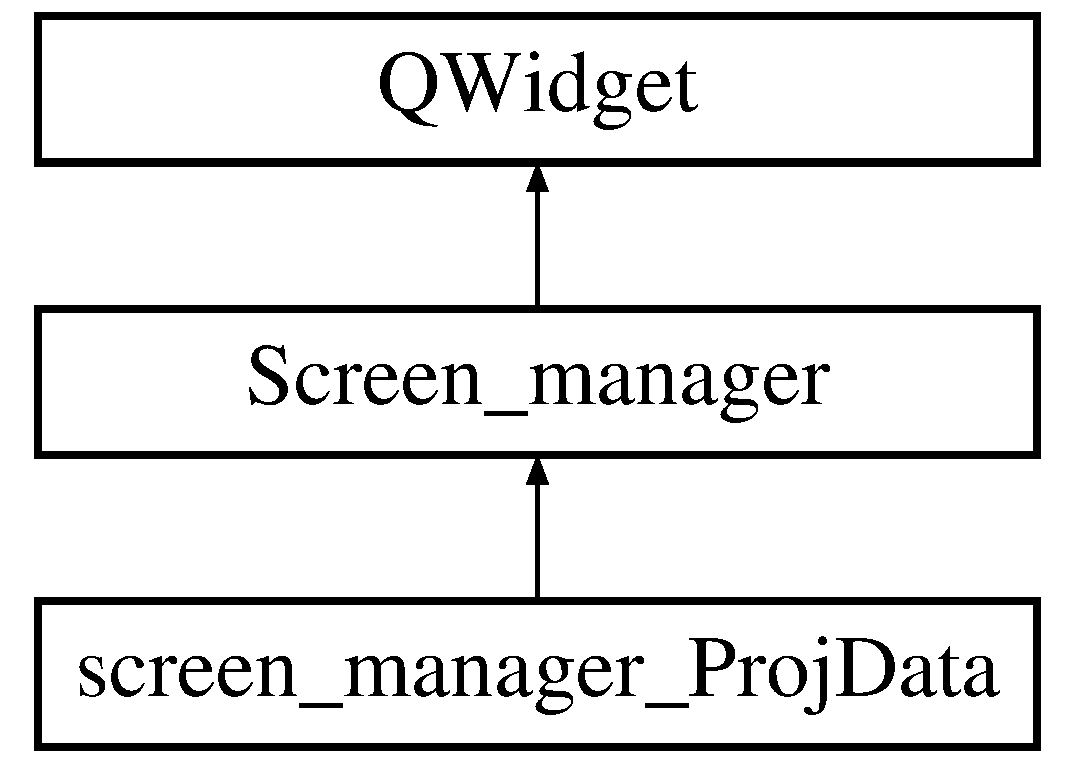
\includegraphics[height=3.000000cm]{classscreen__manager__ProjData}
\end{center}
\end{figure}
\subsection*{Public Slots}
\begin{DoxyCompactItemize}
\item 
void \mbox{\hyperlink{classscreen__manager__ProjData_af999939294c1afe3d7cf218402599de7}{remote\+\_\+segment\+\_\+change}} (Q\+String index)
\begin{DoxyCompactList}\small\item\em remote\+\_\+segment\+\_\+change \end{DoxyCompactList}\item 
\mbox{\Hypertarget{classscreen__manager__ProjData_a05a40e2c5e6272a531ba689764e1a413}\label{classscreen__manager__ProjData_a05a40e2c5e6272a531ba689764e1a413}} 
void {\bfseries on\+Cursor\+Changed} ()
\item 
\mbox{\Hypertarget{classscreen__manager__ProjData_ad921b197a380634d679fb86bc342d032}\label{classscreen__manager__ProjData_ad921b197a380634d679fb86bc342d032}} 
virtual void {\bfseries \+\_\+set\+Cursor} (const Q\+Point \&, Qwt\+Plot $\ast$)
\item 
\mbox{\Hypertarget{classscreen__manager__ProjData_aed563d1a8aa51b0236c237e5c1e140c8}\label{classscreen__manager__ProjData_aed563d1a8aa51b0236c237e5c1e140c8}} 
virtual void {\bfseries \+\_\+set\+Cursor} (const \mbox{\hyperlink{classViewer_1_1SimpleVector3D}{Viewer\+::\+Simple\+Vector3D}}$<$ int $>$ \&)
\item 
\mbox{\Hypertarget{classscreen__manager__ProjData_a6b39c66330e5fdc44c7871af0b37d2c4}\label{classscreen__manager__ProjData_a6b39c66330e5fdc44c7871af0b37d2c4}} 
virtual void {\bfseries update\+Cursor} (\mbox{\hyperlink{classdisplay__screen__container}{display\+\_\+screen\+\_\+container}} $\ast$d=0)
\item 
\mbox{\Hypertarget{classScreen__manager_ac91e8b023e12dc15f8c6ab1951b4ce70}\label{classScreen__manager_ac91e8b023e12dc15f8c6ab1951b4ce70}} 
void {\bfseries remote\+\_\+scrbr\+\_\+value\+Changed} (const qint16 \&value)
\item 
\mbox{\Hypertarget{classScreen__manager_acfda6fcca2edd2d2a155b000256dad56}\label{classScreen__manager_acfda6fcca2edd2d2a155b000256dad56}} 
void {\bfseries remote\+\_\+relative\+\_\+scrbr\+\_\+value\+Changed} (qint32 value)
\item 
void \mbox{\hyperlink{classScreen__manager_afc206ddd1fee12c08d890d7a0c4c5fcb}{update\+All}} ()
\item 
void \mbox{\hyperlink{classScreen__manager_a0a17fba71b72fedefed5651b883ed371}{re\+Plot\+Plots}} ()
\item 
void \mbox{\hyperlink{classScreen__manager_a846061886a15cdc0de881976564b02f2}{refresh\+Plots}} ()
\end{DoxyCompactItemize}
\subsection*{Signals}
\begin{DoxyCompactItemize}
\item 
\mbox{\Hypertarget{classScreen__manager_acafc9314a77776acab7fafdca98c8aa6}\label{classScreen__manager_acafc9314a77776acab7fafdca98c8aa6}} 
void {\bfseries about\+To\+Close} ()
\item 
\mbox{\Hypertarget{classScreen__manager_a50d14535914f456dd55feeb2f54607f5}\label{classScreen__manager_a50d14535914f456dd55feeb2f54607f5}} 
void {\bfseries scrolled\+To} (qint16)
\item 
\mbox{\Hypertarget{classScreen__manager_a98ea0e9ea89f3e457b000b6cbabaa9d9}\label{classScreen__manager_a98ea0e9ea89f3e457b000b6cbabaa9d9}} 
void {\bfseries active\+Screen\+Updated} ()
\item 
\mbox{\Hypertarget{classScreen__manager_add6968bd7e6bedd1fe0d56e41e80a9d3}\label{classScreen__manager_add6968bd7e6bedd1fe0d56e41e80a9d3}} 
void \mbox{\hyperlink{classScreen__manager_add6968bd7e6bedd1fe0d56e41e80a9d3}{segment\+Changed\+To}} (Q\+String)
\begin{DoxyCompactList}\small\item\em segment\+Changed\+To This signal is emitted when the segment changes, in order to notify the rest of the group. \end{DoxyCompactList}\item 
\mbox{\Hypertarget{classScreen__manager_af30611f6463cf716bfe68d235a6884b2}\label{classScreen__manager_af30611f6463cf716bfe68d235a6884b2}} 
void {\bfseries set\+Color\+Map} (const qint16 \&)
\item 
\mbox{\Hypertarget{classScreen__manager_aa3779d6d7f3df9fcae204edb6bd03425}\label{classScreen__manager_aa3779d6d7f3df9fcae204edb6bd03425}} 
void {\bfseries updated\+Container} ()
\end{DoxyCompactItemize}
\subsection*{Public Member Functions}
\begin{DoxyCompactItemize}
\item 
\mbox{\Hypertarget{classscreen__manager__ProjData_ac60289abf8958ad664a826f5acb75b79}\label{classscreen__manager__ProjData_ac60289abf8958ad664a826f5acb75b79}} 
{\bfseries screen\+\_\+manager\+\_\+\+Proj\+Data} (\mbox{\hyperlink{classConfiguration}{Configuration}} $\ast$\mbox{\hyperlink{classScreen__manager_add6a20bb797b0a544aed8b84371a4f24}{cur\+Config}}, Q\+Widget $\ast$parent)
\item 
\mbox{\Hypertarget{classscreen__manager__ProjData_ae31f5cec9fa678f9ab450c86f0d92f14}\label{classscreen__manager__ProjData_ae31f5cec9fa678f9ab450c86f0d92f14}} 
virtual bool {\bfseries load\+File} (const Q\+String file\+Name)
\item 
\mbox{\Hypertarget{classscreen__manager__ProjData_a994944bf714e64c14fec83e7a90bde8f}\label{classscreen__manager__ProjData_a994944bf714e64c14fec83e7a90bde8f}} 
bool {\bfseries set\+State} (qint16 new\+View\+Order, qint16 new\+\_\+current\+\_\+id, qint16 new\+\_\+seg\+\_\+num, qint16 new\+\_\+num\+\_\+viewports)
\item 
\mbox{\Hypertarget{classscreen__manager__ProjData_a9959ff321ca719db4885cd455f5e1c85}\label{classscreen__manager__ProjData_a9959ff321ca719db4885cd455f5e1c85}} 
qint16 {\bfseries get\+Current\+Segment\+Number} () const
\item 
\mbox{\Hypertarget{classscreen__manager__ProjData_a9aeab9515cdae43d551dbead36a976b9}\label{classscreen__manager__ProjData_a9aeab9515cdae43d551dbead36a976b9}} 
void {\bfseries set\+\_\+seg\+\_\+index} (qint16 num\+\_\+seg)
\item 
\mbox{\Hypertarget{classscreen__manager__ProjData_a8f06a3f2795233478e3d2fac82f41bff}\label{classscreen__manager__ProjData_a8f06a3f2795233478e3d2fac82f41bff}} 
virtual Q\+Size {\bfseries set\+Orientation} (Orientation \+\_\+o=Next)
\item 
\mbox{\Hypertarget{classscreen__manager__ProjData_a0f256fa37e1bb4f1e85cd1be9cfefe1a}\label{classscreen__manager__ProjData_a0f256fa37e1bb4f1e85cd1be9cfefe1a}} 
virtual Q\+String \mbox{\hyperlink{classscreen__manager__ProjData_a0f256fa37e1bb4f1e85cd1be9cfefe1a}{get\+Data\+Type}} () const
\begin{DoxyCompactList}\small\item\em Returns image\+Data or proj\+Data. \end{DoxyCompactList}\item 
\mbox{\Hypertarget{classscreen__manager__ProjData_a58d3d2f090c5689a97efcb36aa58c15b}\label{classscreen__manager__ProjData_a58d3d2f090c5689a97efcb36aa58c15b}} 
virtual int {\bfseries get\+Num\+Of\+Arrays} ()
\item 
\mbox{\Hypertarget{classscreen__manager__ProjData_a0e1ab26f7564884ba23b3c0ce2142bb5}\label{classscreen__manager__ProjData_a0e1ab26f7564884ba23b3c0ce2142bb5}} 
virtual Array$<$ 2, float $>$ {\bfseries get\+Array2D} (const int \&) const
\item 
\mbox{\Hypertarget{classscreen__manager__ProjData_a4f22db3b2a9ee85009152f25c1a3f0b0}\label{classscreen__manager__ProjData_a4f22db3b2a9ee85009152f25c1a3f0b0}} 
virtual void {\bfseries set\+Array2D} (const Array$<$ 2, float $>$ \&, const int \&)
\item 
\mbox{\Hypertarget{classscreen__manager__ProjData_a850f0d57175aa9673fe824db6e57e952}\label{classscreen__manager__ProjData_a850f0d57175aa9673fe824db6e57e952}} 
virtual void {\bfseries display} ()
\item 
\mbox{\Hypertarget{classscreen__manager__ProjData_ae1fdcefd945f20b14e436dbf90ce1997}\label{classscreen__manager__ProjData_ae1fdcefd945f20b14e436dbf90ce1997}} 
virtual void \mbox{\hyperlink{classscreen__manager__ProjData_ae1fdcefd945f20b14e436dbf90ce1997}{show\+Cursor}} (const bool \&state=false)
\begin{DoxyCompactList}\small\item\em Display a blue cross on the location of current\+Cursor. \end{DoxyCompactList}\item 
\mbox{\Hypertarget{classscreen__manager__ProjData_a44ecc1dfc00cb24a71df9d221e0730d8}\label{classscreen__manager__ProjData_a44ecc1dfc00cb24a71df9d221e0730d8}} 
virtual const Index\+Range$<$ 3 $>$ {\bfseries get\+Ranges3D} ()
\item 
\mbox{\Hypertarget{classscreen__manager__ProjData_a65c0d425c740209a7b4128bc8ab7acd6}\label{classscreen__manager__ProjData_a65c0d425c740209a7b4128bc8ab7acd6}} 
virtual void \mbox{\hyperlink{classscreen__manager__ProjData_a65c0d425c740209a7b4128bc8ab7acd6}{write\+To\+Disk}} (const Q\+String \&)
\begin{DoxyCompactList}\small\item\em Write image to disk using S\+T\+IR functions. \end{DoxyCompactList}\item 
\mbox{\Hypertarget{classscreen__manager__ProjData_af0ad4c677508a9b4448f2bca7e86a1e6}\label{classscreen__manager__ProjData_af0ad4c677508a9b4448f2bca7e86a1e6}} 
void \mbox{\hyperlink{classscreen__manager__ProjData_af0ad4c677508a9b4448f2bca7e86a1e6}{apply\+Viz\+Values\+To\+All\+Containers}} (const double \&\+\_\+min, const double \&\+\_\+max)
\begin{DoxyCompactList}\small\item\em Set the viz\+\_\+min and viz\+\_\+max values at all containers. \end{DoxyCompactList}\item 
\mbox{\Hypertarget{classscreen__manager__ProjData_a45694c58085eb42093ee8457e4c54db5}\label{classscreen__manager__ProjData_a45694c58085eb42093ee8457e4c54db5}} 
virtual void {\bfseries apply\+Function\+To\+All\+Containers} (\mbox{\hyperlink{classWorker}{Worker}} $\ast$\+\_\+w)
\item 
\mbox{\Hypertarget{classscreen__manager__ProjData_a9906e83cad94c9869f7f10a89568c0af}\label{classscreen__manager__ProjData_a9906e83cad94c9869f7f10a89568c0af}} 
virtual void {\bfseries remove\+Function\+To\+All\+Containers} ()
\item 
\mbox{\Hypertarget{classscreen__manager__ProjData_a0545e6a6fc9a32ef01ca1baad5787d9b}\label{classscreen__manager__ProjData_a0545e6a6fc9a32ef01ca1baad5787d9b}} 
virtual Voxels\+On\+Cartesian\+Grid$<$ float $>$ $\ast$ {\bfseries get\+Data\+\_\+ptr} ()
\item 
\mbox{\Hypertarget{classscreen__manager__ProjData_af44186503b9c822764d92c48c9cfe7ca}\label{classscreen__manager__ProjData_af44186503b9c822764d92c48c9cfe7ca}} 
virtual Cartesian\+Coordinate3D$<$ float $>$ $\ast$ \mbox{\hyperlink{classscreen__manager__ProjData_af44186503b9c822764d92c48c9cfe7ca}{get\+Current\+Cursor\+Inmm}} () const
\begin{DoxyCompactList}\small\item\em The current position of the current\+Cursor. \end{DoxyCompactList}\item 
\mbox{\Hypertarget{classScreen__manager_a317d60e000518cd1af48d04dca139f43}\label{classScreen__manager_a317d60e000518cd1af48d04dca139f43}} 
\mbox{\hyperlink{classdisplay__screen__container}{display\+\_\+screen\+\_\+container}} $\ast$ \mbox{\hyperlink{classScreen__manager_a317d60e000518cd1af48d04dca139f43}{get\+Active\+Display\+Screen}} () const
\begin{DoxyCompactList}\small\item\em Returns the currently active container. \end{DoxyCompactList}\item 
\mbox{\Hypertarget{classScreen__manager_a35fad2826491912a33af8f6b5192abc4}\label{classScreen__manager_a35fad2826491912a33af8f6b5192abc4}} 
Q\+String \mbox{\hyperlink{classScreen__manager_a35fad2826491912a33af8f6b5192abc4}{get\+Full\+File\+Path}} () const
\begin{DoxyCompactList}\small\item\em Get the my\+Full\+File\+Name. \end{DoxyCompactList}\item 
\mbox{\Hypertarget{classScreen__manager_acb7b0f59376ccbc2038b832bba22b577}\label{classScreen__manager_acb7b0f59376ccbc2038b832bba22b577}} 
void \mbox{\hyperlink{classScreen__manager_acb7b0f59376ccbc2038b832bba22b577}{set\+Full\+File\+Path}} (const Q\+String \&)
\begin{DoxyCompactList}\small\item\em Set the my\+Full\+File\+Name. \end{DoxyCompactList}\item 
\mbox{\Hypertarget{classScreen__manager_ab773fd2975a54a2baaeb441b2644607d}\label{classScreen__manager_ab773fd2975a54a2baaeb441b2644607d}} 
Q\+String \mbox{\hyperlink{classScreen__manager_ab773fd2975a54a2baaeb441b2644607d}{get\+File\+Name}} () const
\begin{DoxyCompactList}\small\item\em Returns only the file\+Name. \end{DoxyCompactList}\item 
\mbox{\Hypertarget{classScreen__manager_a44503ee6f24482b8d01797503b0d88a8}\label{classScreen__manager_a44503ee6f24482b8d01797503b0d88a8}} 
qint16 \mbox{\hyperlink{classScreen__manager_a44503ee6f24482b8d01797503b0d88a8}{get\+Color\+Map\+Index}} () const
\begin{DoxyCompactList}\small\item\em Returnes the index of the current Color\+Map. \end{DoxyCompactList}\item 
\mbox{\Hypertarget{classScreen__manager_aec8c672544208e60368172e662de815e}\label{classScreen__manager_aec8c672544208e60368172e662de815e}} 
qint16 \mbox{\hyperlink{classScreen__manager_aec8c672544208e60368172e662de815e}{get\+Viewports\+Index}} () const
\item 
Simple\+Vector3D$<$ int $>$ $\ast$ \mbox{\hyperlink{classScreen__manager_a86a2c051954195c03f8718f4e371c221}{get\+Current\+Cursor}} () const
\item 
Cartesian\+Coordinate3D$<$ int $>$ $\ast$ \mbox{\hyperlink{classScreen__manager_a9cb3da1f84299ee2c32e4032e7e19ed1}{get\+Current\+Cursor}} () const
\item 
\mbox{\Hypertarget{classScreen__manager_a6c41fbe3b06a11879010f8cce4488953}\label{classScreen__manager_a6c41fbe3b06a11879010f8cce4488953}} 
const Orientation $\ast$ \mbox{\hyperlink{classScreen__manager_a6c41fbe3b06a11879010f8cce4488953}{get\+Display\+Layout}} () const
\begin{DoxyCompactList}\small\item\em Returns the current display layout. \end{DoxyCompactList}\item 
\mbox{\Hypertarget{classScreen__manager_a15f0b7a953e3a15c46ccff31681f2c8d}\label{classScreen__manager_a15f0b7a953e3a15c46ccff31681f2c8d}} 
void \mbox{\hyperlink{classScreen__manager_a15f0b7a953e3a15c46ccff31681f2c8d}{set\+\_\+num\+\_\+viewports}} (qint16 num)
\item 
\mbox{\Hypertarget{classScreen__manager_ad86ad708eacc70d09ddfea3991c1436a}\label{classScreen__manager_ad86ad708eacc70d09ddfea3991c1436a}} 
void {\bfseries set\+Grouped} (bool)
\item 
\mbox{\Hypertarget{classScreen__manager_a1e9502d390457183eb1924753c3ffbaa}\label{classScreen__manager_a1e9502d390457183eb1924753c3ffbaa}} 
bool {\bfseries is\+Grouped} () const
\item 
\mbox{\Hypertarget{classScreen__manager_a491fb46b4eb96fb363848a1c506528bd}\label{classScreen__manager_a491fb46b4eb96fb363848a1c506528bd}} 
bool {\bfseries operator==} (const \mbox{\hyperlink{classScreen__manager}{Screen\+\_\+manager}} \&other) const
\item 
\mbox{\Hypertarget{classScreen__manager_a5f6269a00491d2dd64f4da8506f37d2f}\label{classScreen__manager_a5f6269a00491d2dd64f4da8506f37d2f}} 
bool {\bfseries operator!=} (const \mbox{\hyperlink{classScreen__manager}{Screen\+\_\+manager}} \&other) const
\item 
\mbox{\Hypertarget{classScreen__manager_a78723343009e85b288d800d9cc19bf80}\label{classScreen__manager_a78723343009e85b288d800d9cc19bf80}} 
\mbox{\hyperlink{classConfiguration}{Configuration}} $\ast$ {\bfseries get\+\_\+configuration} () const
\item 
\mbox{\Hypertarget{classScreen__manager_aad35e109d8d77378eb94605d10426a6f}\label{classScreen__manager_aad35e109d8d77378eb94605d10426a6f}} 
void {\bfseries block\+\_\+activity} (bool state)
\item 
\mbox{\Hypertarget{classScreen__manager_ac859de377f3ac1b7f18a9be9a21c193b}\label{classScreen__manager_ac859de377f3ac1b7f18a9be9a21c193b}} 
double \mbox{\hyperlink{classScreen__manager_ac859de377f3ac1b7f18a9be9a21c193b}{get\+\_\+min\+\_\+value\+\_\+all}} () const
\begin{DoxyCompactList}\small\item\em Return the minimum value of the entire dataset. \end{DoxyCompactList}\item 
\mbox{\Hypertarget{classScreen__manager_a39bc17ac270cdea092e20bed9d3a1e65}\label{classScreen__manager_a39bc17ac270cdea092e20bed9d3a1e65}} 
double \mbox{\hyperlink{classScreen__manager_a39bc17ac270cdea092e20bed9d3a1e65}{get\+\_\+max\+\_\+value\+\_\+all}} () const
\begin{DoxyCompactList}\small\item\em Return the maximum value of the entire dataset. \end{DoxyCompactList}\item 
\mbox{\Hypertarget{classScreen__manager_ad1cd939deb35910262eaa503018ea1b6}\label{classScreen__manager_ad1cd939deb35910262eaa503018ea1b6}} 
void {\bfseries set\+\_\+multiple\+\_\+selections\+\_\+allowed} (bool state)
\item 
\mbox{\Hypertarget{classScreen__manager_afb1943d5f00971d44c607a35d2f14400}\label{classScreen__manager_afb1943d5f00971d44c607a35d2f14400}} 
bool {\bfseries get\+Cursor\+Status} () const
\item 
\mbox{\Hypertarget{classScreen__manager_a2f34df85df98b630cc76c44f95191b0c}\label{classScreen__manager_a2f34df85df98b630cc76c44f95191b0c}} 
double {\bfseries get\+Current\+Value} ()
\end{DoxyCompactItemize}
\subsection*{Public Attributes}
\begin{DoxyCompactItemize}
\item 
\mbox{\Hypertarget{classScreen__manager_ad20150bef59ac873d47c7dccb5062258}\label{classScreen__manager_ad20150bef59ac873d47c7dccb5062258}} 
Q\+Vector$<$ std\+::shared\+\_\+ptr$<$ \mbox{\hyperlink{classdisplay__screen__container}{display\+\_\+screen\+\_\+container}} $>$ $>$ {\bfseries my\+\_\+containers}
\end{DoxyCompactItemize}
\subsection*{Protected Slots}
\begin{DoxyCompactItemize}
\item 
\mbox{\Hypertarget{classScreen__manager_a9f814711fe49f63a404758ffb39f63cc}\label{classScreen__manager_a9f814711fe49f63a404758ffb39f63cc}} 
void {\bfseries set\+Active\+Screen\+Container} (const qint32 \&)
\end{DoxyCompactItemize}
\subsection*{Protected Member Functions}
\begin{DoxyCompactItemize}
\item 
\mbox{\Hypertarget{classscreen__manager__ProjData_a31e255f3712b77fb7e879ce2777da9b3}\label{classscreen__manager__ProjData_a31e255f3712b77fb7e879ce2777da9b3}} 
virtual void {\bfseries initialise\+Plot\+Area} ()
\item 
\mbox{\Hypertarget{classscreen__manager__ProjData_a909deae69f4052b6d4e3829772feac96}\label{classscreen__manager__ProjData_a909deae69f4052b6d4e3829772feac96}} 
virtual void {\bfseries initialise\+\_\+controls\+\_\+for\+\_\+view} ()
\item 
\mbox{\Hypertarget{classscreen__manager__ProjData_a0c8db64a77a136796003970d7cd2c424}\label{classscreen__manager__ProjData_a0c8db64a77a136796003970d7cd2c424}} 
virtual void {\bfseries initialise\+\_\+controls\+\_\+for\+\_\+\+T\+OF} ()
\item 
\mbox{\Hypertarget{classscreen__manager__ProjData_a538cbc6b1064a5cf6f914e140bbcf7a9}\label{classscreen__manager__ProjData_a538cbc6b1064a5cf6f914e140bbcf7a9}} 
virtual void {\bfseries create\+Actions} ()
\item 
\mbox{\Hypertarget{classscreen__manager__ProjData_a60123dd28eaa9b631fc863c71a90cd65}\label{classscreen__manager__ProjData_a60123dd28eaa9b631fc863c71a90cd65}} 
virtual void {\bfseries save\+\_\+as\+\_\+array} (int this\+\_\+label)
\item 
\mbox{\Hypertarget{classscreen__manager__ProjData_aa2d96ab68be728e63c32e21f2eb26763}\label{classscreen__manager__ProjData_aa2d96ab68be728e63c32e21f2eb26763}} 
virtual double {\bfseries get\+Value\+At} (const \mbox{\hyperlink{classViewer_1_1SimpleVector3D}{Simple\+Vector3D}}$<$ int $>$ \+\_\+c)
\item 
virtual void \mbox{\hyperlink{classscreen__manager__ProjData_aafc7c0ce08eb4870d885e8f4a2596e88}{find\+\_\+min\+\_\+value}} (const int \&slice\+Num, Orientation \+\_\+o=All)
\item 
virtual void \mbox{\hyperlink{classscreen__manager__ProjData_a665de828d1b1761f94a07ad63ecdf75f}{find\+\_\+max\+\_\+value}} (const int \&slice\+Num, Orientation \+\_\+o=All)
\item 
\mbox{\Hypertarget{classScreen__manager_a8285b74dd2913a8368aebb8c4aeccee1}\label{classScreen__manager_a8285b74dd2913a8368aebb8c4aeccee1}} 
virtual void {\bfseries set\+\_\+up\+\_\+plot\+\_\+area} ()
\item 
\mbox{\Hypertarget{classScreen__manager_a1e77461fc2c621a338131d25efa28e7a}\label{classScreen__manager_a1e77461fc2c621a338131d25efa28e7a}} 
void {\bfseries close\+Event} (Q\+Close\+Event $\ast$event) override
\item 
\mbox{\Hypertarget{classScreen__manager_ae999da71a66db6ce0ce62216fe20863a}\label{classScreen__manager_ae999da71a66db6ce0ce62216fe20863a}} 
void \mbox{\hyperlink{classScreen__manager_ae999da71a66db6ce0ce62216fe20863a}{set\+Up\+Containers}} (int \+\_\+num=3)
\begin{DoxyCompactList}\small\item\em Initializes the \mbox{\hyperlink{classdisplay__screen__container}{display\+\_\+screen\+\_\+container}}. /todo The default 3 must change to zero. \end{DoxyCompactList}\item 
void \mbox{\hyperlink{classScreen__manager_a5896c354d45b0b4142a76b26f7081787}{clear\+Containers}} ()
\end{DoxyCompactItemize}
\subsection*{Protected Attributes}
\begin{DoxyCompactItemize}
\item 
\mbox{\Hypertarget{classScreen__manager_a08d9ac0f5ff1946873ceafa1c91fd5bf}\label{classScreen__manager_a08d9ac0f5ff1946873ceafa1c91fd5bf}} 
Ui\+::\+Screen\+\_\+manager $\ast$ {\bfseries ui}
\item 
\mbox{\Hypertarget{classScreen__manager_aca1b3a8cf4a318e3c6a90c8886389cc6}\label{classScreen__manager_aca1b3a8cf4a318e3c6a90c8886389cc6}} 
Q\+String {\bfseries my\+Full\+File\+Name}
\item 
\mbox{\Hypertarget{classScreen__manager_a0677c1654b984e635d160189de4c77ad}\label{classScreen__manager_a0677c1654b984e635d160189de4c77ad}} 
Orientation \mbox{\hyperlink{classScreen__manager_a0677c1654b984e635d160189de4c77ad}{view\+Order}}
\begin{DoxyCompactList}\small\item\em The current Orientation on display. Since Orientation\+::\+All. \end{DoxyCompactList}\item 
\mbox{\Hypertarget{classScreen__manager_add6a20bb797b0a544aed8b84371a4f24}\label{classScreen__manager_add6a20bb797b0a544aed8b84371a4f24}} 
\mbox{\hyperlink{classConfiguration}{Configuration}} $\ast$ \mbox{\hyperlink{classScreen__manager_add6a20bb797b0a544aed8b84371a4f24}{cur\+Config}}
\begin{DoxyCompactList}\small\item\em \mbox{\hyperlink{classConfiguration}{Configuration}} doesn\textquotesingle{}t do a lot, yet. \end{DoxyCompactList}\item 
\mbox{\Hypertarget{classScreen__manager_a8b9367dee1bb7f7b76b7c8b7fd219f6c}\label{classScreen__manager_a8b9367dee1bb7f7b76b7c8b7fd219f6c}} 
\mbox{\hyperlink{classViewer_1_1SimpleVector3D}{Simple\+Vector3D}}$<$ int $>$ $\ast$ \mbox{\hyperlink{classScreen__manager_a8b9367dee1bb7f7b76b7c8b7fd219f6c}{current\+Cursor}}
\begin{DoxyCompactList}\small\item\em The current position it is shared as a pointer in the \mbox{\hyperlink{classdisplay__screen__container}{display\+\_\+screen\+\_\+container}}. \end{DoxyCompactList}\item 
\mbox{\Hypertarget{classScreen__manager_ac1552176fcb2eec1f3f71139933b38b6}\label{classScreen__manager_ac1552176fcb2eec1f3f71139933b38b6}} 
\mbox{\hyperlink{classdisplay__screen__container}{display\+\_\+screen\+\_\+container}} $\ast$ \mbox{\hyperlink{classScreen__manager_ac1552176fcb2eec1f3f71139933b38b6}{active\+Screen\+Contrainer}}
\begin{DoxyCompactList}\small\item\em This is the active \mbox{\hyperlink{classdisplay__screen__container}{display\+\_\+screen\+\_\+container}}. \end{DoxyCompactList}\item 
\mbox{\Hypertarget{classScreen__manager_a9aa51b589844972991a3b234ccf17aa4}\label{classScreen__manager_a9aa51b589844972991a3b234ccf17aa4}} 
bool \mbox{\hyperlink{classScreen__manager_a9aa51b589844972991a3b234ccf17aa4}{cursor\+Status}}
\begin{DoxyCompactList}\small\item\em It indicates wether the blue cross is printed on the displays. \end{DoxyCompactList}\item 
\mbox{\Hypertarget{classScreen__manager_ad88254b68805043118c3fb66009bad6b}\label{classScreen__manager_ad88254b68805043118c3fb66009bad6b}} 
bool \mbox{\hyperlink{classScreen__manager_ad88254b68805043118c3fb66009bad6b}{containers\+Ready}}
\begin{DoxyCompactList}\small\item\em True if the containers have been initialized properly. \end{DoxyCompactList}\item 
\mbox{\Hypertarget{classScreen__manager_a65684948bf1429005ea9f1a507d50e49}\label{classScreen__manager_a65684948bf1429005ea9f1a507d50e49}} 
double \mbox{\hyperlink{classScreen__manager_a65684948bf1429005ea9f1a507d50e49}{min\+Value\+All}}
\begin{DoxyCompactList}\small\item\em The minimum value of the entire dataset. \end{DoxyCompactList}\item 
\mbox{\Hypertarget{classScreen__manager_a8d46413c932ecafedb06fd9b0ee1d6b1}\label{classScreen__manager_a8d46413c932ecafedb06fd9b0ee1d6b1}} 
double \mbox{\hyperlink{classScreen__manager_a8d46413c932ecafedb06fd9b0ee1d6b1}{max\+Value\+All}}
\begin{DoxyCompactList}\small\item\em The maximum value of the entire dataset. \end{DoxyCompactList}\end{DoxyCompactItemize}


\subsection{Member Function Documentation}
\mbox{\Hypertarget{classScreen__manager_a5896c354d45b0b4142a76b26f7081787}\label{classScreen__manager_a5896c354d45b0b4142a76b26f7081787}} 
\index{screen\+\_\+manager\+\_\+\+Proj\+Data@{screen\+\_\+manager\+\_\+\+Proj\+Data}!clear\+Containers@{clear\+Containers}}
\index{clear\+Containers@{clear\+Containers}!screen\+\_\+manager\+\_\+\+Proj\+Data@{screen\+\_\+manager\+\_\+\+Proj\+Data}}
\subsubsection{\texorpdfstring{clear\+Containers()}{clearContainers()}}
{\footnotesize\ttfamily void Screen\+\_\+manager\+::clear\+Containers (\begin{DoxyParamCaption}{ }\end{DoxyParamCaption})\hspace{0.3cm}{\ttfamily [protected]}, {\ttfamily [inherited]}}

Erase the \mbox{\hyperlink{classdisplay__screen__container}{display\+\_\+screen\+\_\+container}}. Since I keep all views in memory this might be . \mbox{\Hypertarget{classscreen__manager__ProjData_a665de828d1b1761f94a07ad63ecdf75f}\label{classscreen__manager__ProjData_a665de828d1b1761f94a07ad63ecdf75f}} 
\index{screen\+\_\+manager\+\_\+\+Proj\+Data@{screen\+\_\+manager\+\_\+\+Proj\+Data}!find\+\_\+max\+\_\+value@{find\+\_\+max\+\_\+value}}
\index{find\+\_\+max\+\_\+value@{find\+\_\+max\+\_\+value}!screen\+\_\+manager\+\_\+\+Proj\+Data@{screen\+\_\+manager\+\_\+\+Proj\+Data}}
\subsubsection{\texorpdfstring{find\+\_\+max\+\_\+value()}{find\_max\_value()}}
{\footnotesize\ttfamily void screen\+\_\+manager\+\_\+\+Proj\+Data\+::find\+\_\+max\+\_\+value (\begin{DoxyParamCaption}\item[{const int \&}]{slice\+Num,  }\item[{Orientation}]{\+\_\+o = {\ttfamily All} }\end{DoxyParamCaption})\hspace{0.3cm}{\ttfamily [protected]}, {\ttfamily [virtual]}}

Find the min value of thie dataset if the orientation is set to All. In any other case get the min value of the selected slice. 

Implements \mbox{\hyperlink{classScreen__manager}{Screen\+\_\+manager}}.

\mbox{\Hypertarget{classscreen__manager__ProjData_aafc7c0ce08eb4870d885e8f4a2596e88}\label{classscreen__manager__ProjData_aafc7c0ce08eb4870d885e8f4a2596e88}} 
\index{screen\+\_\+manager\+\_\+\+Proj\+Data@{screen\+\_\+manager\+\_\+\+Proj\+Data}!find\+\_\+min\+\_\+value@{find\+\_\+min\+\_\+value}}
\index{find\+\_\+min\+\_\+value@{find\+\_\+min\+\_\+value}!screen\+\_\+manager\+\_\+\+Proj\+Data@{screen\+\_\+manager\+\_\+\+Proj\+Data}}
\subsubsection{\texorpdfstring{find\+\_\+min\+\_\+value()}{find\_min\_value()}}
{\footnotesize\ttfamily void screen\+\_\+manager\+\_\+\+Proj\+Data\+::find\+\_\+min\+\_\+value (\begin{DoxyParamCaption}\item[{const int \&}]{slice\+Num,  }\item[{Orientation}]{\+\_\+o = {\ttfamily All} }\end{DoxyParamCaption})\hspace{0.3cm}{\ttfamily [protected]}, {\ttfamily [virtual]}}

Find the min value of thie dataset if the orientation is set to All. In any other case get the min value of the selected slice. 

Implements \mbox{\hyperlink{classScreen__manager}{Screen\+\_\+manager}}.

\mbox{\Hypertarget{classScreen__manager_a86a2c051954195c03f8718f4e371c221}\label{classScreen__manager_a86a2c051954195c03f8718f4e371c221}} 
\index{screen\+\_\+manager\+\_\+\+Proj\+Data@{screen\+\_\+manager\+\_\+\+Proj\+Data}!get\+Current\+Cursor@{get\+Current\+Cursor}}
\index{get\+Current\+Cursor@{get\+Current\+Cursor}!screen\+\_\+manager\+\_\+\+Proj\+Data@{screen\+\_\+manager\+\_\+\+Proj\+Data}}
\subsubsection{\texorpdfstring{get\+Current\+Cursor()}{getCurrentCursor()}\hspace{0.1cm}{\footnotesize\ttfamily [1/2]}}
{\footnotesize\ttfamily Simple\+Vector3D$<$ int $>$ $\ast$ Screen\+\_\+manager\+::get\+Current\+Cursor (\begin{DoxyParamCaption}{ }\end{DoxyParamCaption}) const\hspace{0.3cm}{\ttfamily [inline]}, {\ttfamily [inherited]}}

The current position of the current\+Cursor, overloaded function returning \mbox{\hyperlink{classViewer_1_1SimpleVector3D}{Simple\+Vector3\+D$<$int$>$}} \mbox{\Hypertarget{classScreen__manager_a9cb3da1f84299ee2c32e4032e7e19ed1}\label{classScreen__manager_a9cb3da1f84299ee2c32e4032e7e19ed1}} 
\index{screen\+\_\+manager\+\_\+\+Proj\+Data@{screen\+\_\+manager\+\_\+\+Proj\+Data}!get\+Current\+Cursor@{get\+Current\+Cursor}}
\index{get\+Current\+Cursor@{get\+Current\+Cursor}!screen\+\_\+manager\+\_\+\+Proj\+Data@{screen\+\_\+manager\+\_\+\+Proj\+Data}}
\subsubsection{\texorpdfstring{get\+Current\+Cursor()}{getCurrentCursor()}\hspace{0.1cm}{\footnotesize\ttfamily [2/2]}}
{\footnotesize\ttfamily Cartesian\+Coordinate3D$<$int$>$$\ast$ Screen\+\_\+manager\+::get\+Current\+Cursor (\begin{DoxyParamCaption}{ }\end{DoxyParamCaption}) const\hspace{0.3cm}{\ttfamily [inline]}, {\ttfamily [inherited]}}

The current position of the current\+Cursor, overloaded function returning Cartesian\+Coordinate3\+D$<$int$>$ \mbox{\Hypertarget{classScreen__manager_a846061886a15cdc0de881976564b02f2}\label{classScreen__manager_a846061886a15cdc0de881976564b02f2}} 
\index{screen\+\_\+manager\+\_\+\+Proj\+Data@{screen\+\_\+manager\+\_\+\+Proj\+Data}!refresh\+Plots@{refresh\+Plots}}
\index{refresh\+Plots@{refresh\+Plots}!screen\+\_\+manager\+\_\+\+Proj\+Data@{screen\+\_\+manager\+\_\+\+Proj\+Data}}
\subsubsection{\texorpdfstring{refresh\+Plots}{refreshPlots}}
{\footnotesize\ttfamily void Screen\+\_\+manager\+::refresh\+Plots (\begin{DoxyParamCaption}{ }\end{DoxyParamCaption})\hspace{0.3cm}{\ttfamily [slot]}, {\ttfamily [inherited]}}

This is a ligher version of \mbox{\hyperlink{classScreen__manager_a0a17fba71b72fedefed5651b883ed371}{re\+Plot\+Plots()}}, where the plots are replotted without rereading the data. \mbox{\Hypertarget{classscreen__manager__ProjData_af999939294c1afe3d7cf218402599de7}\label{classscreen__manager__ProjData_af999939294c1afe3d7cf218402599de7}} 
\index{screen\+\_\+manager\+\_\+\+Proj\+Data@{screen\+\_\+manager\+\_\+\+Proj\+Data}!remote\+\_\+segment\+\_\+change@{remote\+\_\+segment\+\_\+change}}
\index{remote\+\_\+segment\+\_\+change@{remote\+\_\+segment\+\_\+change}!screen\+\_\+manager\+\_\+\+Proj\+Data@{screen\+\_\+manager\+\_\+\+Proj\+Data}}
\subsubsection{\texorpdfstring{remote\+\_\+segment\+\_\+change}{remote\_segment\_change}}
{\footnotesize\ttfamily void screen\+\_\+manager\+\_\+\+Proj\+Data\+::remote\+\_\+segment\+\_\+change (\begin{DoxyParamCaption}\item[{Q\+String}]{index }\end{DoxyParamCaption})\hspace{0.3cm}{\ttfamily [slot]}}



remote\+\_\+segment\+\_\+change 


\begin{DoxyParams}{Parameters}
{\em index} & Change the segment remotely. \\
\hline
\end{DoxyParams}
\mbox{\Hypertarget{classScreen__manager_a0a17fba71b72fedefed5651b883ed371}\label{classScreen__manager_a0a17fba71b72fedefed5651b883ed371}} 
\index{screen\+\_\+manager\+\_\+\+Proj\+Data@{screen\+\_\+manager\+\_\+\+Proj\+Data}!re\+Plot\+Plots@{re\+Plot\+Plots}}
\index{re\+Plot\+Plots@{re\+Plot\+Plots}!screen\+\_\+manager\+\_\+\+Proj\+Data@{screen\+\_\+manager\+\_\+\+Proj\+Data}}
\subsubsection{\texorpdfstring{re\+Plot\+Plots}{rePlotPlots}}
{\footnotesize\ttfamily void Screen\+\_\+manager\+::re\+Plot\+Plots (\begin{DoxyParamCaption}{ }\end{DoxyParamCaption})\hspace{0.3cm}{\ttfamily [slot]}, {\ttfamily [inherited]}}

Calls display\+\_\+screen\+\_\+container\+::update\+Plot\+Area for every my\+\_\+container. Effectively the data will be reread. \mbox{\Hypertarget{classScreen__manager_afc206ddd1fee12c08d890d7a0c4c5fcb}\label{classScreen__manager_afc206ddd1fee12c08d890d7a0c4c5fcb}} 
\index{screen\+\_\+manager\+\_\+\+Proj\+Data@{screen\+\_\+manager\+\_\+\+Proj\+Data}!update\+All@{update\+All}}
\index{update\+All@{update\+All}!screen\+\_\+manager\+\_\+\+Proj\+Data@{screen\+\_\+manager\+\_\+\+Proj\+Data}}
\subsubsection{\texorpdfstring{update\+All}{updateAll}}
{\footnotesize\ttfamily void Screen\+\_\+manager\+::update\+All (\begin{DoxyParamCaption}{ }\end{DoxyParamCaption})\hspace{0.3cm}{\ttfamily [slot]}, {\ttfamily [inherited]}}

It will recalculate the minimum and maximum values and replot the screens. 

The documentation for this class was generated from the following files\+:\begin{DoxyCompactItemize}
\item 
src/display\+\_\+buildblock/screen\+\_\+manager\+\_\+projdata.\+h\item 
src/display\+\_\+buildblock/screen\+\_\+manager\+\_\+projdata.\+cpp\item 
src/display\+\_\+buildblock/screen\+\_\+manager\+\_\+projdata.\+inl\end{DoxyCompactItemize}

\hypertarget{classViewer_1_1SimpleVector1D}{}\section{Viewer\+:\+:Simple\+Vector1D$<$ T $>$ Class Template Reference}
\label{classViewer_1_1SimpleVector1D}\index{Viewer\+::\+Simple\+Vector1\+D$<$ T $>$@{Viewer\+::\+Simple\+Vector1\+D$<$ T $>$}}


{\ttfamily \#include $<$common.\+h$>$}

Inheritance diagram for Viewer\+:\+:Simple\+Vector1D$<$ T $>$\+:\begin{figure}[H]
\begin{center}
\leavevmode
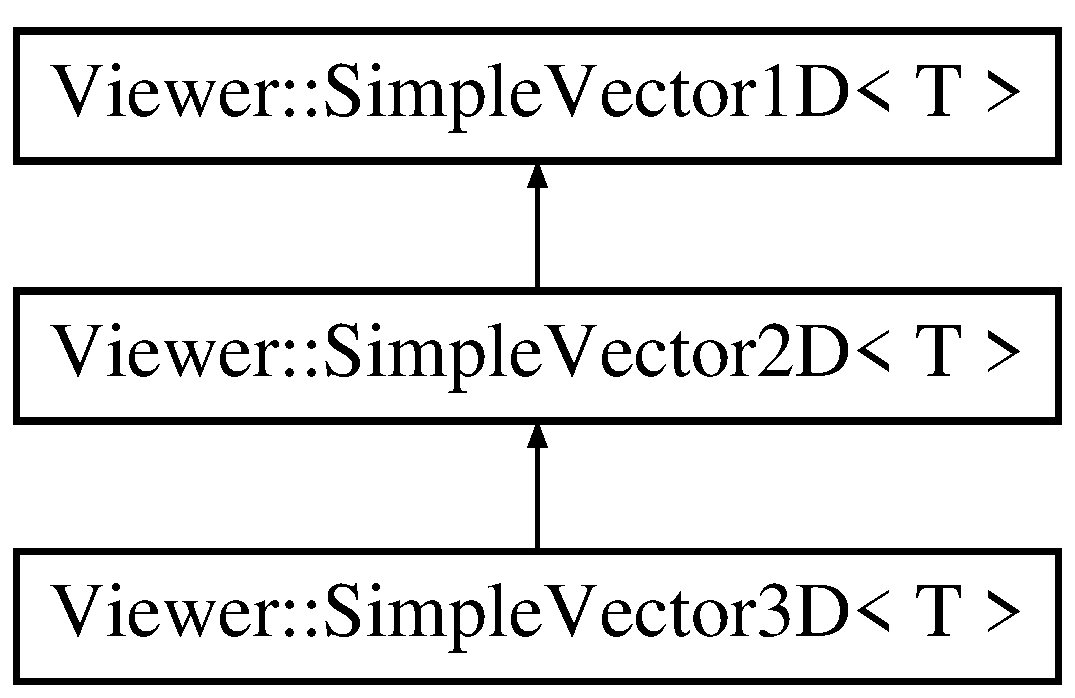
\includegraphics[height=3.000000cm]{classViewer_1_1SimpleVector1D}
\end{center}
\end{figure}
\subsection*{Public Member Functions}
\begin{DoxyCompactItemize}
\item 
\mbox{\Hypertarget{classViewer_1_1SimpleVector1D_acb3334996f977cb906995ebf154a9fa8}\label{classViewer_1_1SimpleVector1D_acb3334996f977cb906995ebf154a9fa8}} 
{\bfseries Simple\+Vector1D} (const T \&\+\_\+x, T \+\_\+o=0.\+0)
\item 
\mbox{\Hypertarget{classViewer_1_1SimpleVector1D_a6b8fdb4e646f7826ce8ccfb41c4c45db}\label{classViewer_1_1SimpleVector1D_a6b8fdb4e646f7826ce8ccfb41c4c45db}} 
void {\bfseries set} (const T \&\+\_\+x)
\item 
\mbox{\Hypertarget{classViewer_1_1SimpleVector1D_ac531dcabcb8b7d26125aedb2bc23a294}\label{classViewer_1_1SimpleVector1D_ac531dcabcb8b7d26125aedb2bc23a294}} 
void {\bfseries set\+Origin} (const T \&\+\_\+o)
\item 
\mbox{\Hypertarget{classViewer_1_1SimpleVector1D_a8b9416bd2f5f50d35b1b9f0adff516eb}\label{classViewer_1_1SimpleVector1D_a8b9416bd2f5f50d35b1b9f0adff516eb}} 
T {\bfseries get\+Eu\+Distance} ()
\end{DoxyCompactItemize}
\subsection*{Public Attributes}
\begin{DoxyCompactItemize}
\item 
\mbox{\Hypertarget{classViewer_1_1SimpleVector1D_a62759b3724abab5ce8ff8d27a56edff6}\label{classViewer_1_1SimpleVector1D_a62759b3724abab5ce8ff8d27a56edff6}} 
T \mbox{\hyperlink{classViewer_1_1SimpleVector1D_a62759b3724abab5ce8ff8d27a56edff6}{x}}
\begin{DoxyCompactList}\small\item\em Terminal Coordinate x. \end{DoxyCompactList}\item 
\mbox{\Hypertarget{classViewer_1_1SimpleVector1D_ac1aa32ecf8bf68483fa1dd9315fc5dbe}\label{classViewer_1_1SimpleVector1D_ac1aa32ecf8bf68483fa1dd9315fc5dbe}} 
T \mbox{\hyperlink{classViewer_1_1SimpleVector1D_ac1aa32ecf8bf68483fa1dd9315fc5dbe}{ox}}
\begin{DoxyCompactList}\small\item\em Origin Coordinate x. \end{DoxyCompactList}\end{DoxyCompactItemize}


\subsection{Detailed Description}
\subsubsection*{template$<$class T$>$\newline
class Viewer\+::\+Simple\+Vector1\+D$<$ T $>$}

Simple template to handle positions. It is often used as cursor. It handles tranformations between Oriantation (s). 

The documentation for this class was generated from the following file\+:\begin{DoxyCompactItemize}
\item 
src/buildblock/common.\+h\end{DoxyCompactItemize}

\hypertarget{classViewer_1_1SimpleVector2D}{}\section{Viewer\+:\+:Simple\+Vector2D$<$ T $>$ Class Template Reference}
\label{classViewer_1_1SimpleVector2D}\index{Viewer\+::\+Simple\+Vector2\+D$<$ T $>$@{Viewer\+::\+Simple\+Vector2\+D$<$ T $>$}}


The 2D version of the \mbox{\hyperlink{classViewer_1_1SimpleVector1D}{Simple\+Vector1D}}.  




{\ttfamily \#include $<$common.\+h$>$}

Inheritance diagram for Viewer\+:\+:Simple\+Vector2D$<$ T $>$\+:\begin{figure}[H]
\begin{center}
\leavevmode
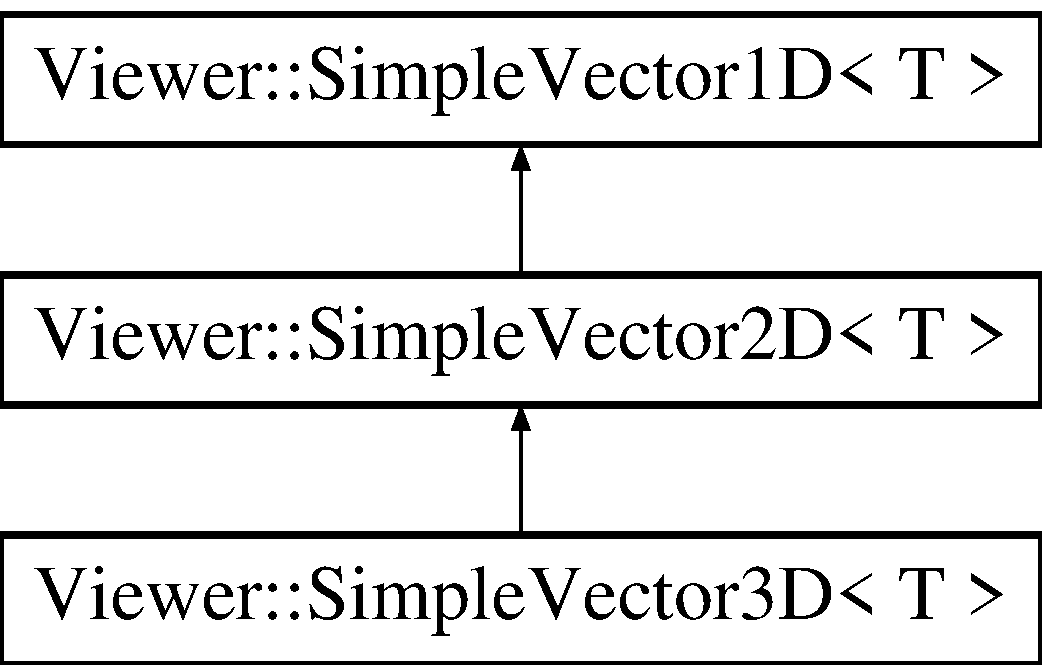
\includegraphics[height=3.000000cm]{classViewer_1_1SimpleVector2D}
\end{center}
\end{figure}
\subsection*{Public Member Functions}
\begin{DoxyCompactItemize}
\item 
\mbox{\Hypertarget{classViewer_1_1SimpleVector2D_a895eedbd1b2acc860c3fc2bb3c733398}\label{classViewer_1_1SimpleVector2D_a895eedbd1b2acc860c3fc2bb3c733398}} 
{\bfseries Simple\+Vector2D} (const T \&\+\_\+x, const T \&\+\_\+y, T \+\_\+ox=0, T \+\_\+oy=0)
\item 
\mbox{\Hypertarget{classViewer_1_1SimpleVector2D_aae8702358d9b0e58f38a8d5e003ba82c}\label{classViewer_1_1SimpleVector2D_aae8702358d9b0e58f38a8d5e003ba82c}} 
{\bfseries Simple\+Vector2D} (const stir\+::\+Cartesian\+Coordinate3D$<$ int $>$ \&\+\_\+c)
\item 
\mbox{\Hypertarget{classViewer_1_1SimpleVector2D_ab1560d4769dad5fa8bd88f34bfdc1beb}\label{classViewer_1_1SimpleVector2D_ab1560d4769dad5fa8bd88f34bfdc1beb}} 
void {\bfseries set} (const T \&\+\_\+x, const T \&\+\_\+y, T \+\_\+ox=0, T \+\_\+oy=0)
\item 
\mbox{\Hypertarget{classViewer_1_1SimpleVector2D_a95e4bbcfc51a28ed3944f378183dcd4d}\label{classViewer_1_1SimpleVector2D_a95e4bbcfc51a28ed3944f378183dcd4d}} 
double {\bfseries get\+Azimuthal\+Angle} ()
\item 
\mbox{\Hypertarget{classViewer_1_1SimpleVector2D_afc891cd6fc33e5bcf8da2494168f6c21}\label{classViewer_1_1SimpleVector2D_afc891cd6fc33e5bcf8da2494168f6c21}} 
Q\+Point {\bfseries to\+Q\+Point} ()
\item 
\mbox{\Hypertarget{classViewer_1_1SimpleVector1D_a6b8fdb4e646f7826ce8ccfb41c4c45db}\label{classViewer_1_1SimpleVector1D_a6b8fdb4e646f7826ce8ccfb41c4c45db}} 
void {\bfseries set} (const T \&\+\_\+x)
\item 
\mbox{\Hypertarget{classViewer_1_1SimpleVector1D_ac531dcabcb8b7d26125aedb2bc23a294}\label{classViewer_1_1SimpleVector1D_ac531dcabcb8b7d26125aedb2bc23a294}} 
void {\bfseries set\+Origin} (const T \&\+\_\+o)
\item 
\mbox{\Hypertarget{classViewer_1_1SimpleVector1D_a8b9416bd2f5f50d35b1b9f0adff516eb}\label{classViewer_1_1SimpleVector1D_a8b9416bd2f5f50d35b1b9f0adff516eb}} 
T {\bfseries get\+Eu\+Distance} ()
\end{DoxyCompactItemize}
\subsection*{Public Attributes}
\begin{DoxyCompactItemize}
\item 
\mbox{\Hypertarget{classViewer_1_1SimpleVector2D_af5a6ca0b14de3c4b62c3e2bcf5ed5012}\label{classViewer_1_1SimpleVector2D_af5a6ca0b14de3c4b62c3e2bcf5ed5012}} 
T \mbox{\hyperlink{classViewer_1_1SimpleVector2D_af5a6ca0b14de3c4b62c3e2bcf5ed5012}{y}}
\begin{DoxyCompactList}\small\item\em Terminal Coordinate y. \end{DoxyCompactList}\item 
\mbox{\Hypertarget{classViewer_1_1SimpleVector2D_a129ba8d14683120474ca46054a9bb5aa}\label{classViewer_1_1SimpleVector2D_a129ba8d14683120474ca46054a9bb5aa}} 
T \mbox{\hyperlink{classViewer_1_1SimpleVector2D_a129ba8d14683120474ca46054a9bb5aa}{oy}}
\begin{DoxyCompactList}\small\item\em ! Origin Coordinate y \end{DoxyCompactList}\item 
\mbox{\Hypertarget{classViewer_1_1SimpleVector1D_a62759b3724abab5ce8ff8d27a56edff6}\label{classViewer_1_1SimpleVector1D_a62759b3724abab5ce8ff8d27a56edff6}} 
T \mbox{\hyperlink{classViewer_1_1SimpleVector1D_a62759b3724abab5ce8ff8d27a56edff6}{x}}
\begin{DoxyCompactList}\small\item\em Terminal Coordinate x. \end{DoxyCompactList}\item 
\mbox{\Hypertarget{classViewer_1_1SimpleVector1D_ac1aa32ecf8bf68483fa1dd9315fc5dbe}\label{classViewer_1_1SimpleVector1D_ac1aa32ecf8bf68483fa1dd9315fc5dbe}} 
T \mbox{\hyperlink{classViewer_1_1SimpleVector1D_ac1aa32ecf8bf68483fa1dd9315fc5dbe}{ox}}
\begin{DoxyCompactList}\small\item\em Origin Coordinate x. \end{DoxyCompactList}\end{DoxyCompactItemize}


\subsection{Detailed Description}
\subsubsection*{template$<$class T$>$\newline
class Viewer\+::\+Simple\+Vector2\+D$<$ T $>$}

The 2D version of the \mbox{\hyperlink{classViewer_1_1SimpleVector1D}{Simple\+Vector1D}}. 

The documentation for this class was generated from the following file\+:\begin{DoxyCompactItemize}
\item 
src/buildblock/common.\+h\end{DoxyCompactItemize}

\hypertarget{classViewer_1_1SimpleVector3D}{}\section{Viewer\+:\+:Simple\+Vector3D$<$ T $>$ Class Template Reference}
\label{classViewer_1_1SimpleVector3D}\index{Viewer\+::\+Simple\+Vector3\+D$<$ T $>$@{Viewer\+::\+Simple\+Vector3\+D$<$ T $>$}}


The 3D version of \mbox{\hyperlink{classViewer_1_1SimpleVector2D}{Simple\+Vector2D}}.  




{\ttfamily \#include $<$common.\+h$>$}

Inheritance diagram for Viewer\+:\+:Simple\+Vector3D$<$ T $>$\+:\begin{figure}[H]
\begin{center}
\leavevmode
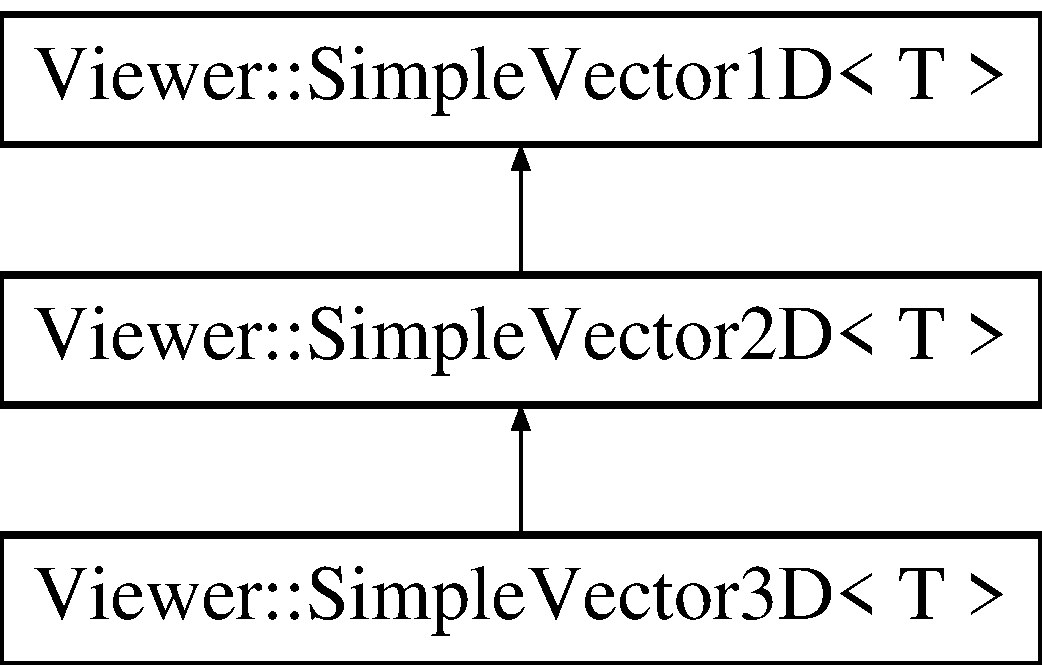
\includegraphics[height=3.000000cm]{classViewer_1_1SimpleVector3D}
\end{center}
\end{figure}
\subsection*{Public Member Functions}
\begin{DoxyCompactItemize}
\item 
\mbox{\Hypertarget{classViewer_1_1SimpleVector3D_a1eef4e84e879f41f7728b9c56bac0be8}\label{classViewer_1_1SimpleVector3D_a1eef4e84e879f41f7728b9c56bac0be8}} 
{\bfseries Simple\+Vector3D} (const T \&\+\_\+x, const T \&\+\_\+y, const T \&\+\_\+z, T \+\_\+ox=0, T \+\_\+oy=0, T \+\_\+oz=0)
\item 
\mbox{\Hypertarget{classViewer_1_1SimpleVector3D_afb1b1a17d5b9c51d0c7ce7e0fcae138e}\label{classViewer_1_1SimpleVector3D_afb1b1a17d5b9c51d0c7ce7e0fcae138e}} 
void {\bfseries set} (const T \&\+\_\+x, const T \&\+\_\+y, const T \&\+\_\+z, T \+\_\+ox=0, T \+\_\+oy=0, T \+\_\+oz=0)
\item 
void \mbox{\hyperlink{classViewer_1_1SimpleVector3D_a124240f41e6e79f30079e9403d1ba75f}{append}} (const Q\+Point \&\+\_\+p, const Orientation $\ast$\+\_\+o)
\item 
void \mbox{\hyperlink{classViewer_1_1SimpleVector3D_af4c356b63832388d9f3a7f6329692ad1}{append}} (const \mbox{\hyperlink{classViewer_1_1SimpleVector2D}{Simple\+Vector2D}}$<$ T $>$ \&\+\_\+p, const Orientation $\ast$\+\_\+o)
\item 
\mbox{\Hypertarget{classViewer_1_1SimpleVector3D_a16d6e68bd050c824b88fdb7ffe064225}\label{classViewer_1_1SimpleVector3D_a16d6e68bd050c824b88fdb7ffe064225}} 
\mbox{\hyperlink{classViewer_1_1SimpleVector2D}{Simple\+Vector2D}}$<$ T $>$ \mbox{\hyperlink{classViewer_1_1SimpleVector3D_a16d6e68bd050c824b88fdb7ffe064225}{get\+Cross}} (Orientation \+\_\+o)
\begin{DoxyCompactList}\small\item\em Reduces the number of dimensions by one w.\+r.\+t the Orientation. \end{DoxyCompactList}\item 
\mbox{\Hypertarget{classViewer_1_1SimpleVector3D_a32c0cbb4c6e62c4f06c1dbfaa6b2c903}\label{classViewer_1_1SimpleVector3D_a32c0cbb4c6e62c4f06c1dbfaa6b2c903}} 
\mbox{\hyperlink{classViewer_1_1SimpleVector1D}{Simple\+Vector1D}}$<$ T $>$ \mbox{\hyperlink{classViewer_1_1SimpleVector3D_a32c0cbb4c6e62c4f06c1dbfaa6b2c903}{get\+Position}} (Orientation \+\_\+o)
\begin{DoxyCompactList}\small\item\em Reduces the number of dimensions by two w.\+r.\+t the Orientation. \end{DoxyCompactList}\item 
\mbox{\Hypertarget{classViewer_1_1SimpleVector3D_a61c728d69f9f2ff817113d7ee2db5b55}\label{classViewer_1_1SimpleVector3D_a61c728d69f9f2ff817113d7ee2db5b55}} 
double {\bfseries get\+Polar\+Angle} ()
\item 
\mbox{\Hypertarget{classViewer_1_1SimpleVector2D_ab1560d4769dad5fa8bd88f34bfdc1beb}\label{classViewer_1_1SimpleVector2D_ab1560d4769dad5fa8bd88f34bfdc1beb}} 
void {\bfseries set} (const T \&\+\_\+x, const T \&\+\_\+y, T \+\_\+ox=0, T \+\_\+oy=0)
\item 
\mbox{\Hypertarget{classViewer_1_1SimpleVector1D_a6b8fdb4e646f7826ce8ccfb41c4c45db}\label{classViewer_1_1SimpleVector1D_a6b8fdb4e646f7826ce8ccfb41c4c45db}} 
void {\bfseries set} (const T \&\+\_\+x)
\item 
\mbox{\Hypertarget{classViewer_1_1SimpleVector2D_a95e4bbcfc51a28ed3944f378183dcd4d}\label{classViewer_1_1SimpleVector2D_a95e4bbcfc51a28ed3944f378183dcd4d}} 
double {\bfseries get\+Azimuthal\+Angle} ()
\item 
\mbox{\Hypertarget{classViewer_1_1SimpleVector2D_afc891cd6fc33e5bcf8da2494168f6c21}\label{classViewer_1_1SimpleVector2D_afc891cd6fc33e5bcf8da2494168f6c21}} 
Q\+Point {\bfseries to\+Q\+Point} ()
\item 
\mbox{\Hypertarget{classViewer_1_1SimpleVector1D_ac531dcabcb8b7d26125aedb2bc23a294}\label{classViewer_1_1SimpleVector1D_ac531dcabcb8b7d26125aedb2bc23a294}} 
void {\bfseries set\+Origin} (const T \&\+\_\+o)
\item 
\mbox{\Hypertarget{classViewer_1_1SimpleVector1D_a8b9416bd2f5f50d35b1b9f0adff516eb}\label{classViewer_1_1SimpleVector1D_a8b9416bd2f5f50d35b1b9f0adff516eb}} 
T {\bfseries get\+Eu\+Distance} ()
\end{DoxyCompactItemize}
\subsection*{Public Attributes}
\begin{DoxyCompactItemize}
\item 
\mbox{\Hypertarget{classViewer_1_1SimpleVector3D_a86e5cf85550e31627b0901df98440013}\label{classViewer_1_1SimpleVector3D_a86e5cf85550e31627b0901df98440013}} 
T \mbox{\hyperlink{classViewer_1_1SimpleVector3D_a86e5cf85550e31627b0901df98440013}{z}}
\begin{DoxyCompactList}\small\item\em Terminal Coordinate z. \end{DoxyCompactList}\item 
\mbox{\Hypertarget{classViewer_1_1SimpleVector3D_a13cdc99dcaaee2e926ea53f728bab398}\label{classViewer_1_1SimpleVector3D_a13cdc99dcaaee2e926ea53f728bab398}} 
T \mbox{\hyperlink{classViewer_1_1SimpleVector3D_a13cdc99dcaaee2e926ea53f728bab398}{oz}}
\begin{DoxyCompactList}\small\item\em Origin Coordinate z. \end{DoxyCompactList}\item 
\mbox{\Hypertarget{classViewer_1_1SimpleVector2D_af5a6ca0b14de3c4b62c3e2bcf5ed5012}\label{classViewer_1_1SimpleVector2D_af5a6ca0b14de3c4b62c3e2bcf5ed5012}} 
T \mbox{\hyperlink{classViewer_1_1SimpleVector2D_af5a6ca0b14de3c4b62c3e2bcf5ed5012}{y}}
\begin{DoxyCompactList}\small\item\em Terminal Coordinate y. \end{DoxyCompactList}\item 
\mbox{\Hypertarget{classViewer_1_1SimpleVector2D_a129ba8d14683120474ca46054a9bb5aa}\label{classViewer_1_1SimpleVector2D_a129ba8d14683120474ca46054a9bb5aa}} 
T \mbox{\hyperlink{classViewer_1_1SimpleVector2D_a129ba8d14683120474ca46054a9bb5aa}{oy}}
\begin{DoxyCompactList}\small\item\em ! Origin Coordinate y \end{DoxyCompactList}\item 
\mbox{\Hypertarget{classViewer_1_1SimpleVector1D_a62759b3724abab5ce8ff8d27a56edff6}\label{classViewer_1_1SimpleVector1D_a62759b3724abab5ce8ff8d27a56edff6}} 
T \mbox{\hyperlink{classViewer_1_1SimpleVector1D_a62759b3724abab5ce8ff8d27a56edff6}{x}}
\begin{DoxyCompactList}\small\item\em Terminal Coordinate x. \end{DoxyCompactList}\item 
\mbox{\Hypertarget{classViewer_1_1SimpleVector1D_ac1aa32ecf8bf68483fa1dd9315fc5dbe}\label{classViewer_1_1SimpleVector1D_ac1aa32ecf8bf68483fa1dd9315fc5dbe}} 
T \mbox{\hyperlink{classViewer_1_1SimpleVector1D_ac1aa32ecf8bf68483fa1dd9315fc5dbe}{ox}}
\begin{DoxyCompactList}\small\item\em Origin Coordinate x. \end{DoxyCompactList}\end{DoxyCompactItemize}


\subsection{Detailed Description}
\subsubsection*{template$<$class T$>$\newline
class Viewer\+::\+Simple\+Vector3\+D$<$ T $>$}

The 3D version of \mbox{\hyperlink{classViewer_1_1SimpleVector2D}{Simple\+Vector2D}}. 

\subsection{Member Function Documentation}
\mbox{\Hypertarget{classViewer_1_1SimpleVector3D_a124240f41e6e79f30079e9403d1ba75f}\label{classViewer_1_1SimpleVector3D_a124240f41e6e79f30079e9403d1ba75f}} 
\index{Viewer\+::\+Simple\+Vector3D@{Viewer\+::\+Simple\+Vector3D}!append@{append}}
\index{append@{append}!Viewer\+::\+Simple\+Vector3D@{Viewer\+::\+Simple\+Vector3D}}
\subsubsection{\texorpdfstring{append()}{append()}\hspace{0.1cm}{\footnotesize\ttfamily [1/2]}}
{\footnotesize\ttfamily template$<$class T$>$ \\
void \mbox{\hyperlink{classViewer_1_1SimpleVector3D}{Viewer\+::\+Simple\+Vector3D}}$<$ T $>$\+::append (\begin{DoxyParamCaption}\item[{const Q\+Point \&}]{\+\_\+p,  }\item[{const Orientation $\ast$}]{\+\_\+o }\end{DoxyParamCaption})\hspace{0.3cm}{\ttfamily [inline]}}

Actually, this is more an asign function but can sort out the Orientation . \mbox{\Hypertarget{classViewer_1_1SimpleVector3D_af4c356b63832388d9f3a7f6329692ad1}\label{classViewer_1_1SimpleVector3D_af4c356b63832388d9f3a7f6329692ad1}} 
\index{Viewer\+::\+Simple\+Vector3D@{Viewer\+::\+Simple\+Vector3D}!append@{append}}
\index{append@{append}!Viewer\+::\+Simple\+Vector3D@{Viewer\+::\+Simple\+Vector3D}}
\subsubsection{\texorpdfstring{append()}{append()}\hspace{0.1cm}{\footnotesize\ttfamily [2/2]}}
{\footnotesize\ttfamily template$<$class T$>$ \\
void \mbox{\hyperlink{classViewer_1_1SimpleVector3D}{Viewer\+::\+Simple\+Vector3D}}$<$ T $>$\+::append (\begin{DoxyParamCaption}\item[{const \mbox{\hyperlink{classViewer_1_1SimpleVector2D}{Simple\+Vector2D}}$<$ T $>$ \&}]{\+\_\+p,  }\item[{const Orientation $\ast$}]{\+\_\+o }\end{DoxyParamCaption})\hspace{0.3cm}{\ttfamily [inline]}}

Actually, this is more an asign function but can sort out the Orientation . 

The documentation for this class was generated from the following file\+:\begin{DoxyCompactItemize}
\item 
src/buildblock/common.\+h\end{DoxyCompactItemize}

\hypertarget{classThresholdMan}{}\section{Threshold\+Man Class Reference}
\label{classThresholdMan}\index{Threshold\+Man@{Threshold\+Man}}
Inheritance diagram for Threshold\+Man\+:\begin{figure}[H]
\begin{center}
\leavevmode
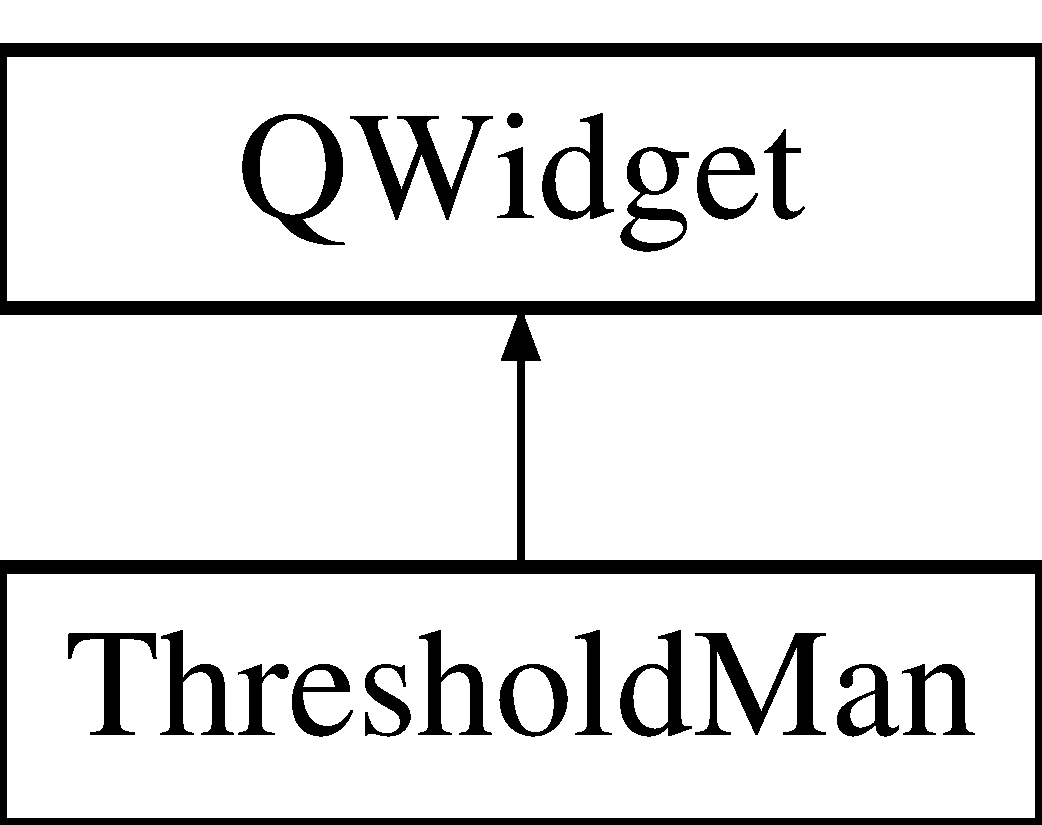
\includegraphics[height=2.000000cm]{classThresholdMan}
\end{center}
\end{figure}
\subsection*{Public Slots}
\begin{DoxyCompactItemize}
\item 
\mbox{\Hypertarget{classThresholdMan_a46424217b012608d39f365fec7881315}\label{classThresholdMan_a46424217b012608d39f365fec7881315}} 
void {\bfseries notify\+Value\+Changed} (int value)
\item 
\mbox{\Hypertarget{classThresholdMan_a35de41fade07efb313b22ccfabcb49c2}\label{classThresholdMan_a35de41fade07efb313b22ccfabcb49c2}} 
void {\bfseries notify\+Int\+Value\+Changed} (double value)
\end{DoxyCompactItemize}
\subsection*{Signals}
\begin{DoxyCompactItemize}
\item 
\mbox{\Hypertarget{classThresholdMan_a08132244c52a0a51d2cd6f4019508e34}\label{classThresholdMan_a08132244c52a0a51d2cd6f4019508e34}} 
void {\bfseries double\+Value\+Changed} (double value)
\item 
\mbox{\Hypertarget{classThresholdMan_a33b5f9611dc6dba2c9fed171d7c35f77}\label{classThresholdMan_a33b5f9611dc6dba2c9fed171d7c35f77}} 
void {\bfseries int\+Value\+Changed} (int value)
\end{DoxyCompactItemize}
\subsection*{Public Member Functions}
\begin{DoxyCompactItemize}
\item 
\mbox{\Hypertarget{classThresholdMan_a6a5c7632349045654bf3c8fcb3f16e85}\label{classThresholdMan_a6a5c7632349045654bf3c8fcb3f16e85}} 
{\bfseries Threshold\+Man} (\mbox{\hyperlink{classScreen__manager}{Screen\+\_\+manager}} $\ast$\+\_\+p, Q\+Widget $\ast$parent=0)
\item 
float \mbox{\hyperlink{classThresholdMan_a86ada2cb5a498fe86616031d1f5e0fc8}{get\+Threshold\+Value}} ()
\end{DoxyCompactItemize}
\subsection*{Protected Attributes}
\begin{DoxyCompactItemize}
\item 
\mbox{\Hypertarget{classThresholdMan_a56c9f2cd7a3c484871206c4c21e446b5}\label{classThresholdMan_a56c9f2cd7a3c484871206c4c21e446b5}} 
\mbox{\hyperlink{classScreen__manager}{Screen\+\_\+manager}} $\ast$ {\bfseries sc}
\item 
\mbox{\Hypertarget{classThresholdMan_acb9ba537b13a1e0b6cf4dbed0dc23a1e}\label{classThresholdMan_acb9ba537b13a1e0b6cf4dbed0dc23a1e}} 
\mbox{\hyperlink{classBarScreenHistogram}{Bar\+Screen\+Histogram}} $\ast$ \mbox{\hyperlink{classThresholdMan_acb9ba537b13a1e0b6cf4dbed0dc23a1e}{my\+\_\+histogram}}
\begin{DoxyCompactList}\small\item\em The histogram to display the selection. \end{DoxyCompactList}\item 
\mbox{\Hypertarget{classThresholdMan_ae437bf23f0a7132b592ab2d7016ca2ad}\label{classThresholdMan_ae437bf23f0a7132b592ab2d7016ca2ad}} 
\mbox{\hyperlink{classWorkerThresholder}{Worker\+Thresholder}} $\ast$ \mbox{\hyperlink{classThresholdMan_ae437bf23f0a7132b592ab2d7016ca2ad}{preview\+\_\+thresholder}}
\begin{DoxyCompactList}\small\item\em The \mbox{\hyperlink{classWorker}{Worker}} that performs the operation. \end{DoxyCompactList}\end{DoxyCompactItemize}


\subsection{Member Function Documentation}
\mbox{\Hypertarget{classThresholdMan_a86ada2cb5a498fe86616031d1f5e0fc8}\label{classThresholdMan_a86ada2cb5a498fe86616031d1f5e0fc8}} 
\index{Threshold\+Man@{Threshold\+Man}!get\+Threshold\+Value@{get\+Threshold\+Value}}
\index{get\+Threshold\+Value@{get\+Threshold\+Value}!Threshold\+Man@{Threshold\+Man}}
\subsubsection{\texorpdfstring{get\+Threshold\+Value()}{getThresholdValue()}}
{\footnotesize\ttfamily float Threshold\+Man\+::get\+Threshold\+Value (\begin{DoxyParamCaption}{ }\end{DoxyParamCaption})}

Depending on wether manual or Otsu operation this function will return the appropriate threshold value. 

The documentation for this class was generated from the following files\+:\begin{DoxyCompactItemize}
\item 
src/ui\+\_\+buildblock/thresholdman.\+h\item 
src/ui\+\_\+buildblock/thresholdman.\+cpp\end{DoxyCompactItemize}

\hypertarget{classTool}{}\section{Tool Class Reference}
\label{classTool}\index{Tool@{Tool}}


{\ttfamily \#include $<$tool.\+h$>$}

Inheritance diagram for Tool\+:\begin{figure}[H]
\begin{center}
\leavevmode
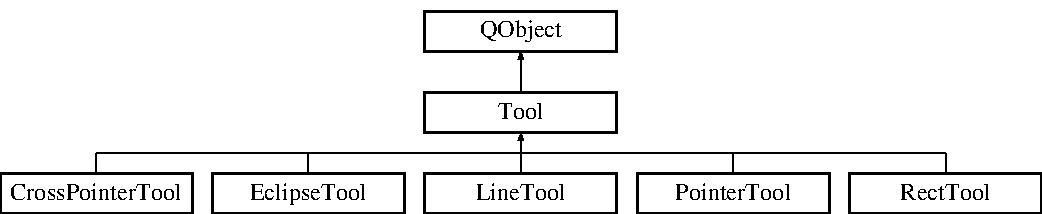
\includegraphics[height=2.871795cm]{classTool}
\end{center}
\end{figure}
\subsection*{Signals}
\begin{DoxyCompactItemize}
\item 
\mbox{\Hypertarget{classTool_a68dea3e4c911f3174176084d350865cc}\label{classTool_a68dea3e4c911f3174176084d350865cc}} 
void {\bfseries this\+\_\+selection} (const Q\+Vector$<$ Q\+PointF $>$ \&, Qwt\+Plot $\ast$)
\end{DoxyCompactItemize}
\subsection*{Public Member Functions}
\begin{DoxyCompactItemize}
\item 
\mbox{\Hypertarget{classTool_a1f72e991d5b5656fd532340b064f4ca5}\label{classTool_a1f72e991d5b5656fd532340b064f4ca5}} 
{\bfseries Tool} (Q\+Widget $\ast$parent=0)
\item 
\mbox{\Hypertarget{classTool_a020bd5757a03ea7321848a3874f3a8cb}\label{classTool_a020bd5757a03ea7321848a3874f3a8cb}} 
virtual bool {\bfseries event\+Filter} (Q\+Object $\ast$, Q\+Event $\ast$)
\item 
\mbox{\Hypertarget{classTool_aa30c64915020a71d0ea8650e8e966336}\label{classTool_aa30c64915020a71d0ea8650e8e966336}} 
virtual Q\+String {\bfseries get\+\_\+name} () const
\item 
\mbox{\Hypertarget{classTool_a5cb18e4c28ab3d8d39535db5d2213c81}\label{classTool_a5cb18e4c28ab3d8d39535db5d2213c81}} 
virtual void {\bfseries finished\+Selecting} ()=0
\item 
\mbox{\Hypertarget{classTool_a507adfcdafc818d9628b952001b93f3c}\label{classTool_a507adfcdafc818d9628b952001b93f3c}} 
void {\bfseries get\+\_\+data} (Q\+Vector$<$ Q\+PointF $>$ \&, Qwt\+Plot $\ast$)
\item 
virtual void \mbox{\hyperlink{classTool_a7d9e7d03f4a34d71850cbbfc16ca8532}{clear\+Before\+Un\+Set}} ()=0
\end{DoxyCompactItemize}
\subsection*{Protected Member Functions}
\begin{DoxyCompactItemize}
\item 
\mbox{\Hypertarget{classTool_a11f1da4092d196a7b91d3d60276586eb}\label{classTool_a11f1da4092d196a7b91d3d60276586eb}} 
virtual void \mbox{\hyperlink{classTool_a11f1da4092d196a7b91d3d60276586eb}{clear\+Selection}} ()
\begin{DoxyCompactList}\small\item\em Remove all curves from the c\+\_\+paint\+Device. \end{DoxyCompactList}\item 
bool \mbox{\hyperlink{classTool_a81244366dc1b9f55465ed6f37b81033c}{check\+Point\+In\+Range}} (const Q\+PointF \&\+\_\+local)
\item 
\mbox{\Hypertarget{classTool_a453549f925313d28b19fc9a81aabfe01}\label{classTool_a453549f925313d28b19fc9a81aabfe01}} 
virtual void \mbox{\hyperlink{classTool_a453549f925313d28b19fc9a81aabfe01}{select}} (const Q\+PointF \&)=0
\begin{DoxyCompactList}\small\item\em On mouse press action. \end{DoxyCompactList}\item 
\mbox{\Hypertarget{classTool_a734b60b6ecf4b9fa2e56186349a5a3cf}\label{classTool_a734b60b6ecf4b9fa2e56186349a5a3cf}} 
virtual void \mbox{\hyperlink{classTool_a734b60b6ecf4b9fa2e56186349a5a3cf}{move}} (const Q\+PointF \&)=0
\begin{DoxyCompactList}\small\item\em On mouse press and drag action. \end{DoxyCompactList}\end{DoxyCompactItemize}
\subsection*{Protected Attributes}
\begin{DoxyCompactItemize}
\item 
\mbox{\Hypertarget{classTool_af0935d8e8edd73d8ec85424b5b15196b}\label{classTool_af0935d8e8edd73d8ec85424b5b15196b}} 
Q\+String {\bfseries name}
\item 
\mbox{\Hypertarget{classTool_a1e301a03c5806c900786760d80049380}\label{classTool_a1e301a03c5806c900786760d80049380}} 
Qwt\+Plot\+Canvas $\ast$ {\bfseries c\+\_\+paint\+Device}
\item 
\mbox{\Hypertarget{classTool_af1d11cc5374ba7eb7c1d41cfb5d4e981}\label{classTool_af1d11cc5374ba7eb7c1d41cfb5d4e981}} 
Qwt\+Plot\+Spectrogram $\ast$ {\bfseries d\+\_\+spectrogram}
\item 
Q\+Vector$<$ Q\+PointF $>$ \mbox{\hyperlink{classTool_a68be77a2e364a7b13d7206388ba5843e}{\+\_\+points}}
\end{DoxyCompactItemize}


\subsection{Detailed Description}
This is the base class for all paint tools 

\subsection{Member Function Documentation}
\mbox{\Hypertarget{classTool_a81244366dc1b9f55465ed6f37b81033c}\label{classTool_a81244366dc1b9f55465ed6f37b81033c}} 
\index{Tool@{Tool}!check\+Point\+In\+Range@{check\+Point\+In\+Range}}
\index{check\+Point\+In\+Range@{check\+Point\+In\+Range}!Tool@{Tool}}
\subsubsection{\texorpdfstring{check\+Point\+In\+Range()}{checkPointInRange()}}
{\footnotesize\ttfamily bool Tool\+::check\+Point\+In\+Range (\begin{DoxyParamCaption}\item[{const Q\+PointF \&}]{\+\_\+local }\end{DoxyParamCaption})\hspace{0.3cm}{\ttfamily [protected]}}

This is a preliminiry check to see if the point is within the axis range. It has been proven somewhat week condition, as in many cases it fails to provide realible results. \mbox{\Hypertarget{classTool_a7d9e7d03f4a34d71850cbbfc16ca8532}\label{classTool_a7d9e7d03f4a34d71850cbbfc16ca8532}} 
\index{Tool@{Tool}!clear\+Before\+Un\+Set@{clear\+Before\+Un\+Set}}
\index{clear\+Before\+Un\+Set@{clear\+Before\+Un\+Set}!Tool@{Tool}}
\subsubsection{\texorpdfstring{clear\+Before\+Un\+Set()}{clearBeforeUnSet()}}
{\footnotesize\ttfamily virtual void Tool\+::clear\+Before\+Un\+Set (\begin{DoxyParamCaption}{ }\end{DoxyParamCaption})\hspace{0.3cm}{\ttfamily [pure virtual]}}

Cal this function to clean before unsetting a tool. It will try to tight up the screen. 

Implemented in \mbox{\hyperlink{classPointerTool_a04c325128dc9ee27272eace9e70d15aa}{Pointer\+Tool}}, \mbox{\hyperlink{classLineTool_a2bcf5d5694e36445607c68c37e4f3f69}{Line\+Tool}}, \mbox{\hyperlink{classCrossPointerTool_a99e1b8f0669837dc5524c446e3dd401c}{Cross\+Pointer\+Tool}}, and \mbox{\hyperlink{classRectTool_a22ddb88797de61ed921a5cd3462383ea}{Rect\+Tool}}.



\subsection{Member Data Documentation}
\mbox{\Hypertarget{classTool_a68be77a2e364a7b13d7206388ba5843e}\label{classTool_a68be77a2e364a7b13d7206388ba5843e}} 
\index{Tool@{Tool}!\+\_\+points@{\+\_\+points}}
\index{\+\_\+points@{\+\_\+points}!Tool@{Tool}}
\subsubsection{\texorpdfstring{\+\_\+points}{\_points}}
{\footnotesize\ttfamily Q\+Vector$<$Q\+PointF$>$ Tool\+::\+\_\+points\hspace{0.3cm}{\ttfamily [protected]}}

This vector holds the characteristic points of the selected R\+OI. The \mbox{\hyperlink{classCrossPointerTool}{Cross\+Pointer\+Tool}} has just one point. The \mbox{\hyperlink{classLineTool}{Line\+Tool}} has two points (e.\+g. start and stop) e.\+t.\+c 

The documentation for this class was generated from the following files\+:\begin{DoxyCompactItemize}
\item 
src/tools\+\_\+buildblock/tool.\+h\item 
src/tools\+\_\+buildblock/tool.\+cpp\end{DoxyCompactItemize}

\hypertarget{classToolManager}{}\section{Tool\+Manager Class Reference}
\label{classToolManager}\index{Tool\+Manager@{Tool\+Manager}}
Inheritance diagram for Tool\+Manager\+:\begin{figure}[H]
\begin{center}
\leavevmode
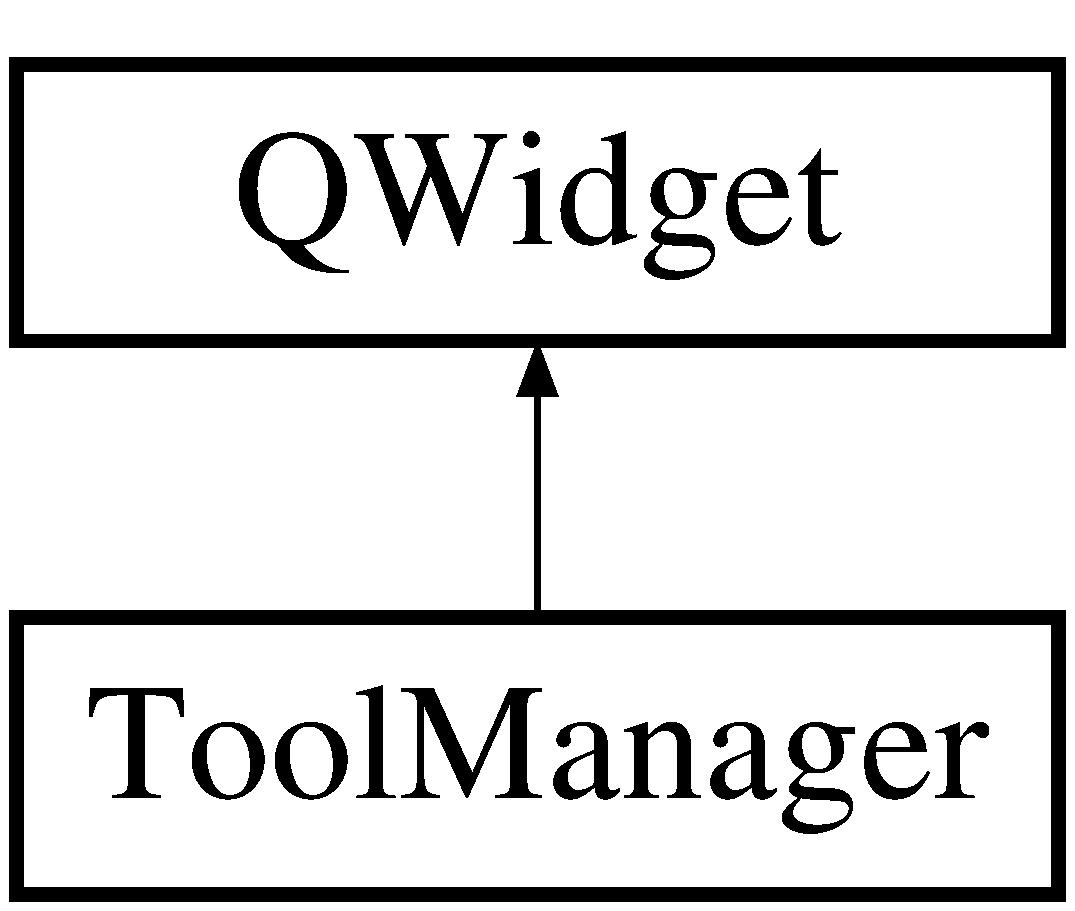
\includegraphics[height=2.000000cm]{classToolManager}
\end{center}
\end{figure}
\subsection*{Public Slots}
\begin{DoxyCompactItemize}
\item 
\mbox{\Hypertarget{classToolManager_a7ca8d129c5ec26d50650bd94962c3339}\label{classToolManager_a7ca8d129c5ec26d50650bd94962c3339}} 
void {\bfseries update\+Menus} (Q\+Widget $\ast$\+\_\+w=0)
\end{DoxyCompactItemize}
\subsection*{Signals}
\begin{DoxyCompactItemize}
\item 
\mbox{\Hypertarget{classToolManager_aa2f5d9b90348fc40dbffe14561323c36}\label{classToolManager_aa2f5d9b90348fc40dbffe14561323c36}} 
void {\bfseries tool\+\_\+selected} (std\+::shared\+\_\+ptr$<$ \mbox{\hyperlink{classTool}{Tool}} $>$)
\end{DoxyCompactItemize}
\subsection*{Public Member Functions}
\begin{DoxyCompactItemize}
\item 
\mbox{\Hypertarget{classToolManager_a545deb9764ae2e7a3f400c5cbb39ad97}\label{classToolManager_a545deb9764ae2e7a3f400c5cbb39ad97}} 
{\bfseries Tool\+Manager} (Q\+Widget $\ast$parent=0)
\item 
\mbox{\Hypertarget{classToolManager_af014405a887ece8d7f1b9f615cf23ba9}\label{classToolManager_af014405a887ece8d7f1b9f615cf23ba9}} 
std\+::shared\+\_\+ptr$<$ \mbox{\hyperlink{classPointerTool}{Pointer\+Tool}} $>$ {\bfseries mouse\+Pointer} () const
\item 
\mbox{\Hypertarget{classToolManager_aa3d042011bef91da4b62abba3ed57bf5}\label{classToolManager_aa3d042011bef91da4b62abba3ed57bf5}} 
std\+::shared\+\_\+ptr$<$ \mbox{\hyperlink{classLineTool}{Line\+Tool}} $>$ {\bfseries mouse\+Line\+Pointer} () const
\item 
\mbox{\Hypertarget{classToolManager_ac41a1125038d46a2f58340a7c4618b29}\label{classToolManager_ac41a1125038d46a2f58340a7c4618b29}} 
std\+::shared\+\_\+ptr$<$ \mbox{\hyperlink{classCrossPointerTool}{Cross\+Pointer\+Tool}} $>$ {\bfseries mouse\+Cross\+Pointer} () const
\item 
\mbox{\Hypertarget{classToolManager_a30041d36e599e0eb5026130c4bfede93}\label{classToolManager_a30041d36e599e0eb5026130c4bfede93}} 
std\+::shared\+\_\+ptr$<$ \mbox{\hyperlink{classRectTool}{Rect\+Tool}} $>$ {\bfseries mouse\+Rect\+Pointer} () const
\item 
\mbox{\Hypertarget{classToolManager_ab7e6dfe68ed07dc91dbfafc2c12f4621}\label{classToolManager_ab7e6dfe68ed07dc91dbfafc2c12f4621}} 
std\+::shared\+\_\+ptr$<$ \mbox{\hyperlink{classTool}{Tool}} $>$ {\bfseries get\+Current\+Tool} () const
\item 
\mbox{\Hypertarget{classToolManager_acf037bd364532b9bf2dec9564ec630f7}\label{classToolManager_acf037bd364532b9bf2dec9564ec630f7}} 
void {\bfseries set\+Screen} (\mbox{\hyperlink{classScreen__manager}{Screen\+\_\+manager}} $\ast$\+\_\+s)
\item 
\mbox{\Hypertarget{classToolManager_a3f3257e4c8d3cc407b734438a99dba3e}\label{classToolManager_a3f3257e4c8d3cc407b734438a99dba3e}} 
void {\bfseries unset\+Screen} ()
\item 
Pixels\+On\+Cartesian\+Grid$<$ float $>$ \mbox{\hyperlink{classToolManager_a2b92398db6ca45c14b28bc54fbe4d64a}{get\+Selection}} () const
\end{DoxyCompactItemize}
\subsection*{Protected Attributes}
\begin{DoxyCompactItemize}
\item 
\mbox{\Hypertarget{classToolManager_a04210d43878f8b154b927b3d88e4415c}\label{classToolManager_a04210d43878f8b154b927b3d88e4415c}} 
\mbox{\hyperlink{classScreen__manager}{Screen\+\_\+manager}} $\ast$ {\bfseries sc}
\end{DoxyCompactItemize}


\subsection{Member Function Documentation}
\mbox{\Hypertarget{classToolManager_a2b92398db6ca45c14b28bc54fbe4d64a}\label{classToolManager_a2b92398db6ca45c14b28bc54fbe4d64a}} 
\index{Tool\+Manager@{Tool\+Manager}!get\+Selection@{get\+Selection}}
\index{get\+Selection@{get\+Selection}!Tool\+Manager@{Tool\+Manager}}
\subsubsection{\texorpdfstring{get\+Selection()}{getSelection()}}
{\footnotesize\ttfamily Pixels\+On\+Cartesian\+Grid$<$ float $>$ Tool\+Manager\+::get\+Selection (\begin{DoxyParamCaption}{ }\end{DoxyParamCaption}) const}

Returns the current selection. If no selection has been made the full slice will return. 

The documentation for this class was generated from the following files\+:\begin{DoxyCompactItemize}
\item 
src/tools\+\_\+buildblock/Tool\+Manager.\+h\item 
src/tools\+\_\+buildblock/Tool\+Manager.\+cpp\item 
src/tools\+\_\+buildblock/Tool\+Manager.\+inl\end{DoxyCompactItemize}

\hypertarget{classWorker}{}\section{Worker Class Reference}
\label{classWorker}\index{Worker@{Worker}}
Inheritance diagram for Worker\+:\begin{figure}[H]
\begin{center}
\leavevmode
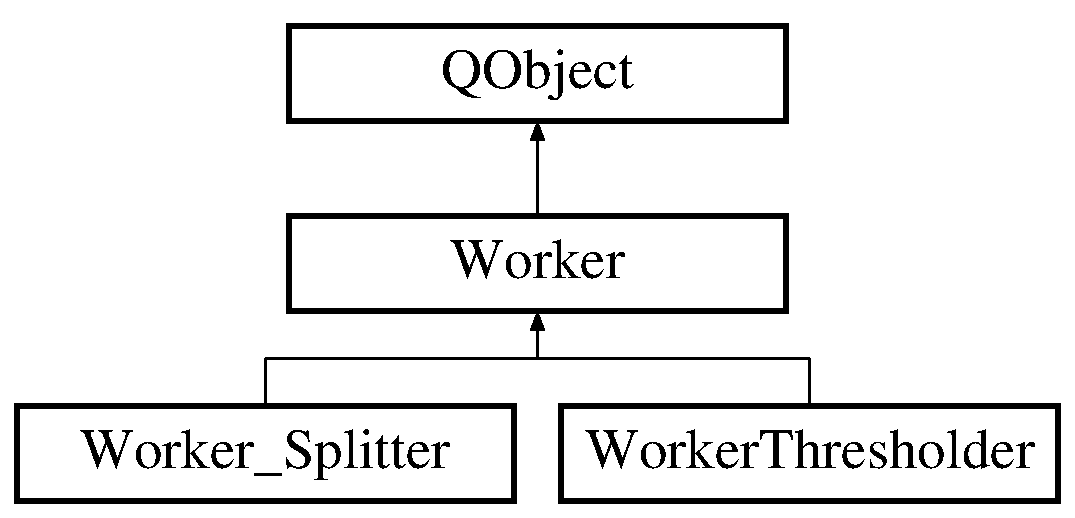
\includegraphics[height=3.000000cm]{classWorker}
\end{center}
\end{figure}
\subsection*{Public Slots}
\begin{DoxyCompactItemize}
\item 
\mbox{\Hypertarget{classWorker_abee6689b3ecc44de33d55dfae0a6af97}\label{classWorker_abee6689b3ecc44de33d55dfae0a6af97}} 
virtual void {\bfseries process} ()=0
\end{DoxyCompactItemize}
\subsection*{Signals}
\begin{DoxyCompactItemize}
\item 
\mbox{\Hypertarget{classWorker_a95f9f660a4f74f24ae5b8470fa1e4050}\label{classWorker_a95f9f660a4f74f24ae5b8470fa1e4050}} 
void {\bfseries result\+Ready} ()
\end{DoxyCompactItemize}
\subsection*{Public Member Functions}
\begin{DoxyCompactItemize}
\item 
\mbox{\Hypertarget{classWorker_a3290234525f8aad4f10f73305c9d1859}\label{classWorker_a3290234525f8aad4f10f73305c9d1859}} 
{\bfseries Worker} (Q\+Object $\ast$parent=0)
\item 
\mbox{\Hypertarget{classWorker_abb9cbb7748f7ce26ec78b9ae561e72d6}\label{classWorker_abb9cbb7748f7ce26ec78b9ae561e72d6}} 
virtual void {\bfseries apply} (Q\+Vector$<$ double $>$ \&d)=0
\end{DoxyCompactItemize}


The documentation for this class was generated from the following files\+:\begin{DoxyCompactItemize}
\item 
src/tools\+\_\+buildblock/worker.\+h\item 
src/tools\+\_\+buildblock/worker.\+cpp\end{DoxyCompactItemize}

\hypertarget{classWorker__Splitter}{}\section{Worker\+\_\+\+Splitter Class Reference}
\label{classWorker__Splitter}\index{Worker\+\_\+\+Splitter@{Worker\+\_\+\+Splitter}}
Inheritance diagram for Worker\+\_\+\+Splitter\+:\begin{figure}[H]
\begin{center}
\leavevmode
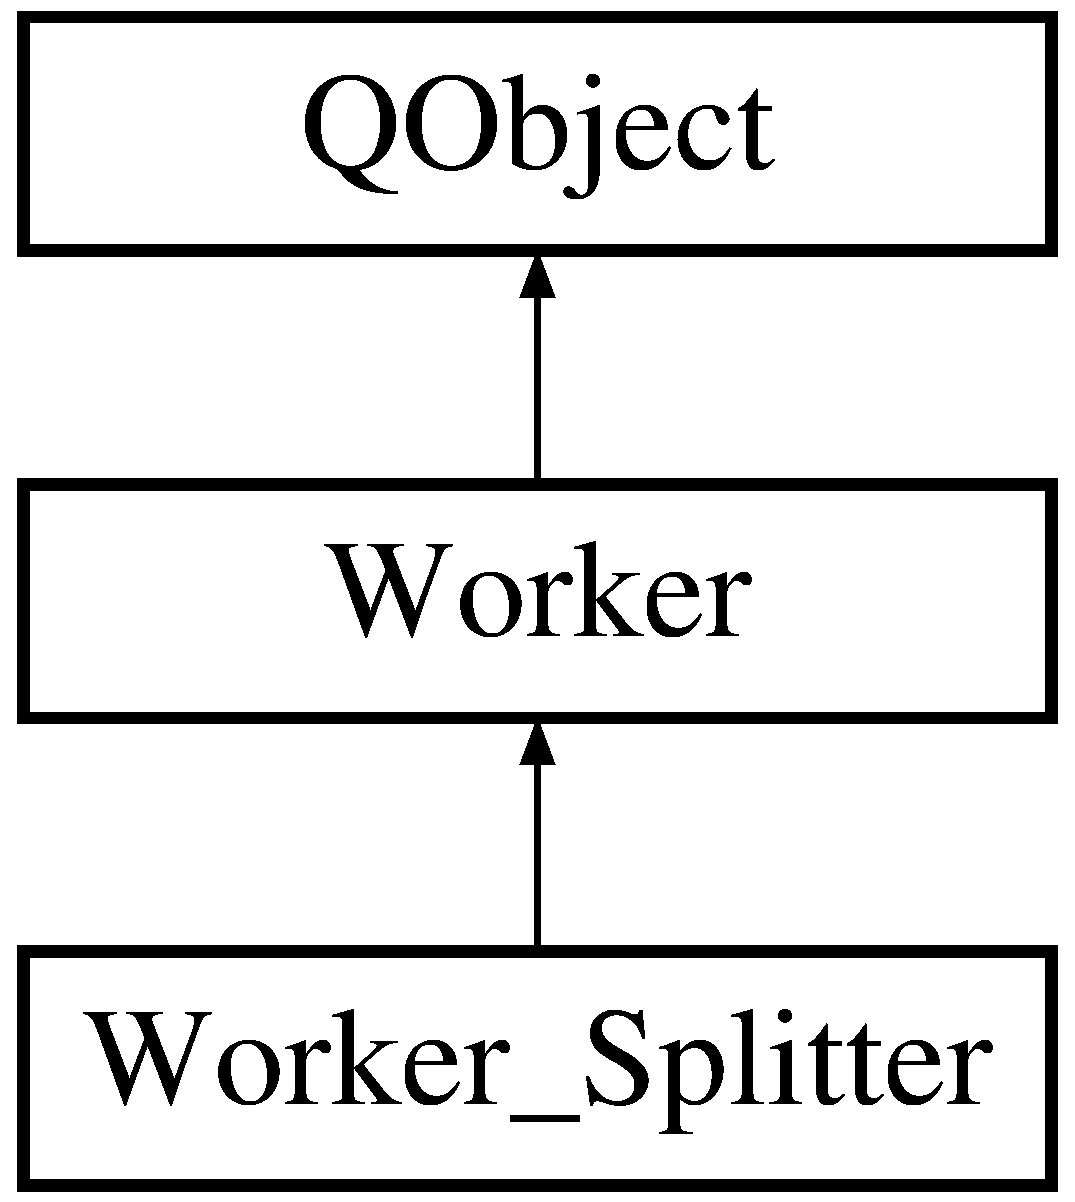
\includegraphics[height=3.000000cm]{classWorker__Splitter}
\end{center}
\end{figure}
\subsection*{Public Slots}
\begin{DoxyCompactItemize}
\item 
\mbox{\Hypertarget{classWorker__Splitter_affc7c9660d9fea2948add9c1a60baa84}\label{classWorker__Splitter_affc7c9660d9fea2948add9c1a60baa84}} 
virtual void {\bfseries process} ()
\end{DoxyCompactItemize}
\subsection*{Signals}
\begin{DoxyCompactItemize}
\item 
\mbox{\Hypertarget{classWorker_a95f9f660a4f74f24ae5b8470fa1e4050}\label{classWorker_a95f9f660a4f74f24ae5b8470fa1e4050}} 
void {\bfseries result\+Ready} ()
\end{DoxyCompactItemize}
\subsection*{Public Member Functions}
\begin{DoxyCompactItemize}
\item 
\mbox{\Hypertarget{classWorker__Splitter_a15c799c0805dc73f2238f2f7cf1a3b7c}\label{classWorker__Splitter_a15c799c0805dc73f2238f2f7cf1a3b7c}} 
{\bfseries Worker\+\_\+\+Splitter} (Q\+Widget $\ast$parent=0)
\item 
\mbox{\Hypertarget{classWorker__Splitter_a3aeba8122c3902784eaefcb11009ba21}\label{classWorker__Splitter_a3aeba8122c3902784eaefcb11009ba21}} 
void {\bfseries set\+Spit\+Slide} (const int \&\+\_\+s)
\item 
\mbox{\Hypertarget{classWorker__Splitter_af06a8ff739af01c614867610a9a9008c}\label{classWorker__Splitter_af06a8ff739af01c614867610a9a9008c}} 
virtual void {\bfseries apply} (Q\+Vector$<$ double $>$ \&d)
\item 
\mbox{\Hypertarget{classWorker__Splitter_a3fbda2dcd55fe3b4b63308d2f0e36e8b}\label{classWorker__Splitter_a3fbda2dcd55fe3b4b63308d2f0e36e8b}} 
void {\bfseries set\+Data} (Voxels\+On\+Cartesian\+Grid$<$ float $>$ $\ast$\+\_\+d)
\end{DoxyCompactItemize}
\subsection*{Public Attributes}
\begin{DoxyCompactItemize}
\item 
\mbox{\Hypertarget{classWorker__Splitter_a34221e79228bc2702c3c31d68d885ebd}\label{classWorker__Splitter_a34221e79228bc2702c3c31d68d885ebd}} 
Q\+Vector$<$ Voxels\+On\+Cartesian\+Grid$<$ float $>$ $>$ {\bfseries split\+\_\+list}
\end{DoxyCompactItemize}


The documentation for this class was generated from the following files\+:\begin{DoxyCompactItemize}
\item 
src/tools\+\_\+buildblock/worker\+\_\+splitter.\+h\item 
src/tools\+\_\+buildblock/worker\+\_\+splitter.\+cpp\end{DoxyCompactItemize}

\hypertarget{classWorkerManager}{}\section{Worker\+Manager Class Reference}
\label{classWorkerManager}\index{Worker\+Manager@{Worker\+Manager}}
Inheritance diagram for Worker\+Manager\+:\begin{figure}[H]
\begin{center}
\leavevmode
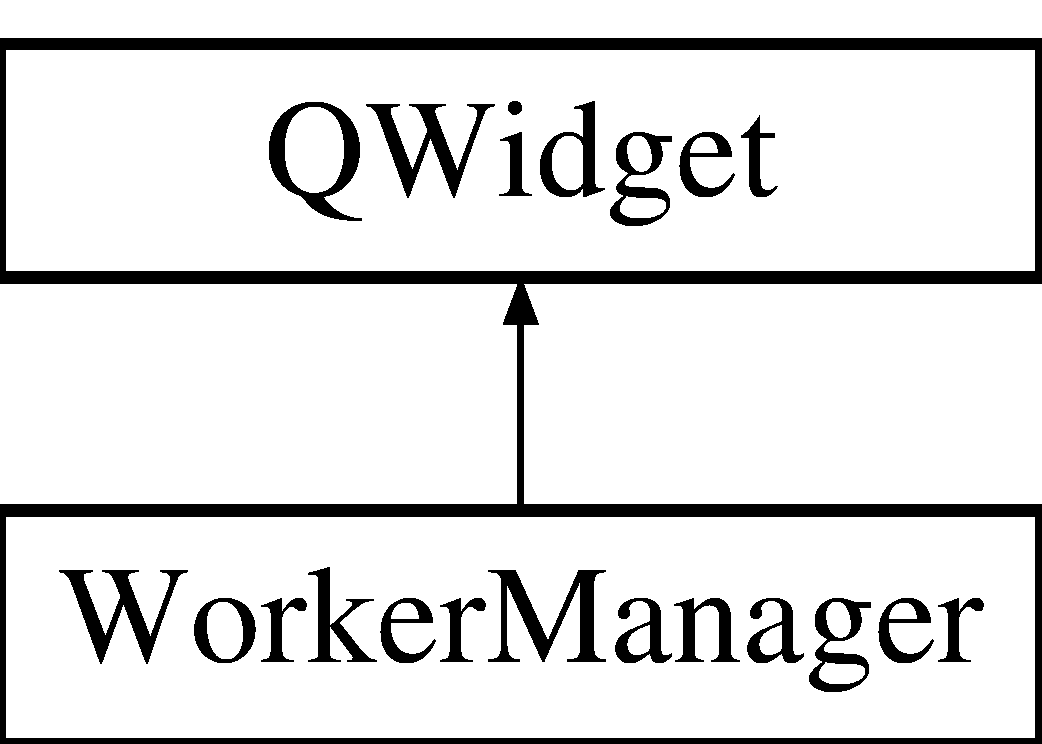
\includegraphics[height=2.000000cm]{classWorkerManager}
\end{center}
\end{figure}
\subsection*{Public Member Functions}
\begin{DoxyCompactItemize}
\item 
\mbox{\Hypertarget{classWorkerManager_ad04a87bc7a60cea19c8ba5f480812a96}\label{classWorkerManager_ad04a87bc7a60cea19c8ba5f480812a96}} 
{\bfseries Worker\+Manager} (Q\+Widget $\ast$parent=0)
\item 
\mbox{\Hypertarget{classWorkerManager_a10a8c619bf754a0c7cf8f8ac49b406fc}\label{classWorkerManager_a10a8c619bf754a0c7cf8f8ac49b406fc}} 
void {\bfseries append\+To\+Queue} ()
\end{DoxyCompactItemize}


The documentation for this class was generated from the following files\+:\begin{DoxyCompactItemize}
\item 
src/tools\+\_\+buildblock/workermanager.\+h\item 
src/tools\+\_\+buildblock/workermanager.\+cpp\end{DoxyCompactItemize}

\hypertarget{classWorkerThresholder}{}\section{Worker\+Thresholder Class Reference}
\label{classWorkerThresholder}\index{Worker\+Thresholder@{Worker\+Thresholder}}
Inheritance diagram for Worker\+Thresholder\+:\begin{figure}[H]
\begin{center}
\leavevmode
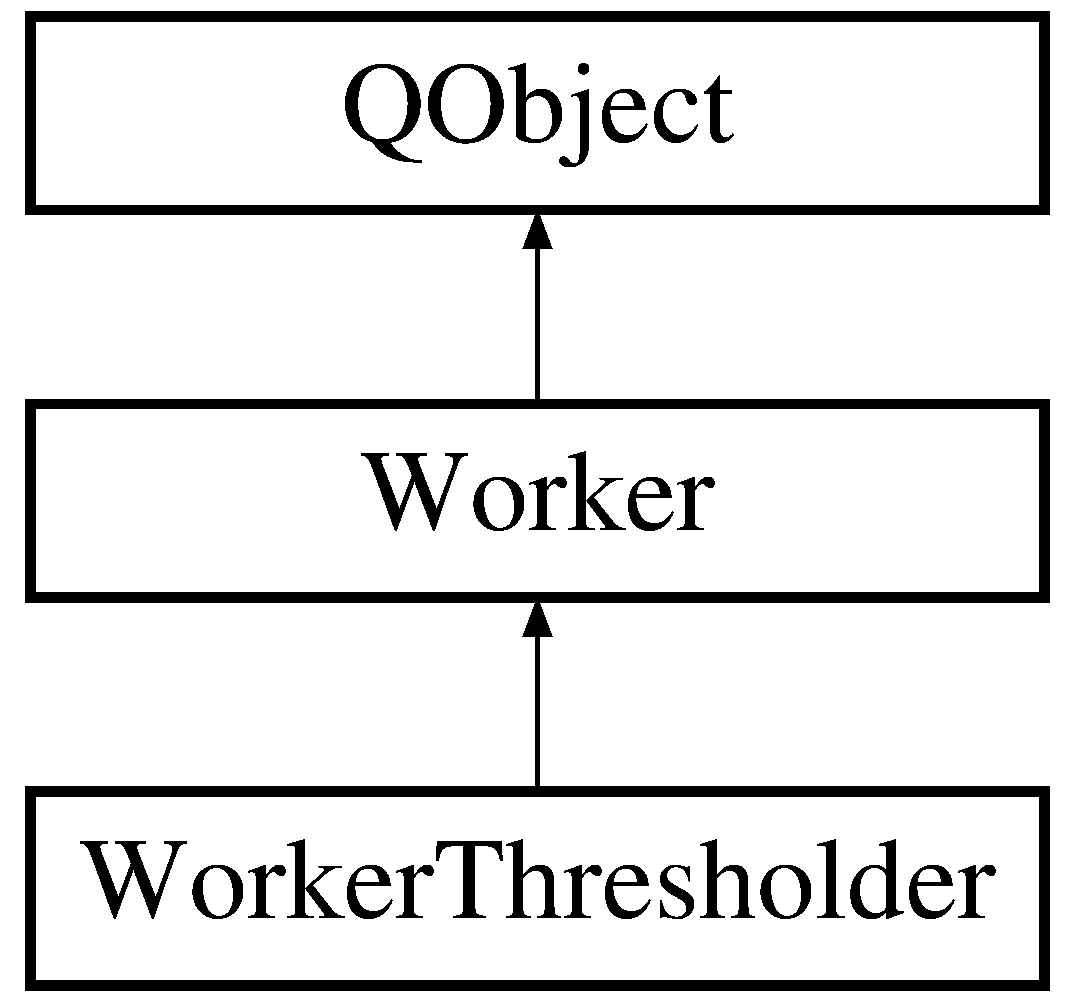
\includegraphics[height=3.000000cm]{classWorkerThresholder}
\end{center}
\end{figure}
\subsection*{Public Slots}
\begin{DoxyCompactItemize}
\item 
\mbox{\Hypertarget{classWorkerThresholder_a22be27a9baa201b1da78bd320f0611e4}\label{classWorkerThresholder_a22be27a9baa201b1da78bd320f0611e4}} 
virtual void {\bfseries process} ()
\end{DoxyCompactItemize}
\subsection*{Signals}
\begin{DoxyCompactItemize}
\item 
\mbox{\Hypertarget{classWorker_a95f9f660a4f74f24ae5b8470fa1e4050}\label{classWorker_a95f9f660a4f74f24ae5b8470fa1e4050}} 
void {\bfseries result\+Ready} ()
\end{DoxyCompactItemize}
\subsection*{Public Member Functions}
\begin{DoxyCompactItemize}
\item 
\mbox{\Hypertarget{classWorkerThresholder_a35cbae7e9e8de11ba7e45b8afafb9d38}\label{classWorkerThresholder_a35cbae7e9e8de11ba7e45b8afafb9d38}} 
{\bfseries Worker\+Thresholder} (Q\+Object $\ast$parent=0)
\item 
\mbox{\Hypertarget{classWorkerThresholder_a3399c8df444f36872f081049b3561320}\label{classWorkerThresholder_a3399c8df444f36872f081049b3561320}} 
{\bfseries Worker\+Thresholder} (Array$<$ 2, float $>$, const float \&thres, Q\+Object $\ast$parent=0)
\item 
\mbox{\Hypertarget{classWorkerThresholder_a40ff8486408c1da75630055f85e2c2db}\label{classWorkerThresholder_a40ff8486408c1da75630055f85e2c2db}} 
{\bfseries Worker\+Thresholder} (const float \&thes, Q\+Object $\ast$parent=0)
\item 
\mbox{\Hypertarget{classWorkerThresholder_ac7890d8abc4f09aa820259485ab7143e}\label{classWorkerThresholder_ac7890d8abc4f09aa820259485ab7143e}} 
void {\bfseries set\+Thres\+Value} (const double \&\+\_\+v)
\item 
\mbox{\Hypertarget{classWorkerThresholder_a996b4c40e4b94c53a087263f44aedfc4}\label{classWorkerThresholder_a996b4c40e4b94c53a087263f44aedfc4}} 
void {\bfseries set\+Mask} (const bool \&\+\_\+v)
\item 
\mbox{\Hypertarget{classWorkerThresholder_a37f2dd82a4606065c60f3c95951e7b60}\label{classWorkerThresholder_a37f2dd82a4606065c60f3c95951e7b60}} 
virtual void {\bfseries apply} (Q\+Vector$<$ double $>$ \&d)
\item 
\mbox{\Hypertarget{classWorkerThresholder_a3c38c0c582ce9a7976d39127c92ff359}\label{classWorkerThresholder_a3c38c0c582ce9a7976d39127c92ff359}} 
Q\+Vector$<$ float $>$ {\bfseries get\+Result} ()
\end{DoxyCompactItemize}


The documentation for this class was generated from the following files\+:\begin{DoxyCompactItemize}
\item 
src/tools\+\_\+buildblock/worker\+\_\+thresholder.\+h\item 
src/tools\+\_\+buildblock/worker\+\_\+thresholder.\+cpp\end{DoxyCompactItemize}

%--- End generated contents ---

% Index
\backmatter
\newpage
\phantomsection
\clearemptydoublepage
\addcontentsline{toc}{chapter}{Index}
\printindex

\end{document}
